\documentclass[twoside]{book}

% Packages required by doxygen
\usepackage{fixltx2e}
\usepackage{calc}
\usepackage{doxygen}
\usepackage[export]{adjustbox} % also loads graphicx
\usepackage{graphicx}
\usepackage[utf8]{inputenc}
\usepackage{makeidx}
\usepackage{multicol}
\usepackage{multirow}
\PassOptionsToPackage{warn}{textcomp}
\usepackage{textcomp}
\usepackage[nointegrals]{wasysym}
\usepackage[table]{xcolor}

% Font selection
\usepackage[T1]{fontenc}
\usepackage[scaled=.90]{helvet}
\usepackage{courier}
\usepackage{amssymb}
\usepackage{sectsty}
\renewcommand{\familydefault}{\sfdefault}
\allsectionsfont{%
  \fontseries{bc}\selectfont%
  \color{darkgray}%
}
\renewcommand{\DoxyLabelFont}{%
  \fontseries{bc}\selectfont%
  \color{darkgray}%
}
\newcommand{\+}{\discretionary{\mbox{\scriptsize$\hookleftarrow$}}{}{}}

% Page & text layout
\usepackage{geometry}
\geometry{%
  a4paper,%
  top=2.5cm,%
  bottom=2.5cm,%
  left=2.5cm,%
  right=2.5cm%
}
\tolerance=750
\hfuzz=15pt
\hbadness=750
\setlength{\emergencystretch}{15pt}
\setlength{\parindent}{0cm}
\setlength{\parskip}{3ex plus 2ex minus 2ex}
\makeatletter
\renewcommand{\paragraph}{%
  \@startsection{paragraph}{4}{0ex}{-1.0ex}{1.0ex}{%
    \normalfont\normalsize\bfseries\SS@parafont%
  }%
}
\renewcommand{\subparagraph}{%
  \@startsection{subparagraph}{5}{0ex}{-1.0ex}{1.0ex}{%
    \normalfont\normalsize\bfseries\SS@subparafont%
  }%
}
\makeatother

% Headers & footers
\usepackage{fancyhdr}
\pagestyle{fancyplain}
\fancyhead[LE]{\fancyplain{}{\bfseries\thepage}}
\fancyhead[CE]{\fancyplain{}{}}
\fancyhead[RE]{\fancyplain{}{\bfseries\leftmark}}
\fancyhead[LO]{\fancyplain{}{\bfseries\rightmark}}
\fancyhead[CO]{\fancyplain{}{}}
\fancyhead[RO]{\fancyplain{}{\bfseries\thepage}}
\fancyfoot[LE]{\fancyplain{}{}}
\fancyfoot[CE]{\fancyplain{}{}}
\fancyfoot[RE]{\fancyplain{}{\bfseries\scriptsize Generated by Doxygen }}
\fancyfoot[LO]{\fancyplain{}{\bfseries\scriptsize Generated by Doxygen }}
\fancyfoot[CO]{\fancyplain{}{}}
\fancyfoot[RO]{\fancyplain{}{}}
\renewcommand{\footrulewidth}{0.4pt}
\renewcommand{\chaptermark}[1]{%
  \markboth{#1}{}%
}
\renewcommand{\sectionmark}[1]{%
  \markright{\thesection\ #1}%
}

% Indices & bibliography
\usepackage{natbib}
\usepackage[titles]{tocloft}
\setcounter{tocdepth}{3}
\setcounter{secnumdepth}{5}
\makeindex

% Hyperlinks (required, but should be loaded last)
\usepackage{ifpdf}
\ifpdf
  \usepackage[pdftex,pagebackref=true]{hyperref}
\else
  \usepackage[ps2pdf,pagebackref=true]{hyperref}
\fi
\hypersetup{%
  colorlinks=true,%
  linkcolor=blue,%
  citecolor=blue,%
  unicode%
}

% Custom commands
\newcommand{\clearemptydoublepage}{%
  \newpage{\pagestyle{empty}\cleardoublepage}%
}

\usepackage{caption}
\captionsetup{labelsep=space,justification=centering,font={bf},singlelinecheck=off,skip=4pt,position=top}

%===== C O N T E N T S =====

\begin{document}

% Titlepage & ToC
\hypersetup{pageanchor=false,
             bookmarksnumbered=true,
             pdfencoding=unicode
            }
\pagenumbering{roman}
\begin{titlepage}
\vspace*{7cm}
\begin{center}%
{\Large My Project }\\
\vspace*{1cm}
{\large Generated by Doxygen 1.8.11}\\
\end{center}
\end{titlepage}
\clearemptydoublepage
\tableofcontents
\clearemptydoublepage
\pagenumbering{arabic}
\hypersetup{pageanchor=true}

%--- Begin generated contents ---
\chapter{Thread safe queue.}
\label{md_project_Readme}
\hypertarget{md_project_Readme}{}
To develop a class which allows to read/write/modify data inside in a thread safety mode. To use for this purpose c++11 standard or greater. The class should be templated (the type of data to work with is a template parameter).

\subsection*{Functional requirements}


\begin{DoxyItemize}
\item to read/write internal state into file system
\item data interaction/modification should be prioritized
\item tests coverage
\item benchmarks
\item if queue is full or empty return false (non blocking method) immediately. 
\end{DoxyItemize}
\chapter{Namespace Index}
\section{Namespace List}
Here is a list of all namespaces with brief descriptions\+:\begin{DoxyCompactList}
\item\contentsline{section}{\hyperlink{namespaceGraphicalEditorCore}{Graphical\+Editor\+Core} }{\pageref{namespaceGraphicalEditorCore}}{}
\item\contentsline{section}{\hyperlink{namespacestd}{std} }{\pageref{namespacestd}}{}
\end{DoxyCompactList}

\chapter{Hierarchical Index}
\section{Class Hierarchy}
This inheritance list is sorted roughly, but not completely, alphabetically\+:\begin{DoxyCompactList}
\item \contentsline{section}{are\+\_\+types\+\_\+same$<$ Args $>$}{\pageref{structare__types__same}}{}
\item \contentsline{section}{are\+\_\+types\+\_\+same$<$ T $>$}{\pageref{structare__types__same_3_01T_01_4}}{}
\item \contentsline{section}{are\+\_\+types\+\_\+same$<$ T, U, Args... $>$}{\pageref{structare__types__same_3_01T_00_01U_00_01Args_8_8_8_01_4}}{}
\item \contentsline{section}{are\+\_\+types\+\_\+same$<$$>$}{\pageref{structare__types__same_3_4}}{}
\item \contentsline{section}{contigious\+\_\+block$<$ T $>$}{\pageref{classcontigious__block}}{}
\item \contentsline{section}{custom\+\_\+tuple$<$ Types $>$}{\pageref{structcustom__tuple}}{}
\item \contentsline{section}{custom\+\_\+tuple$<$ Types... $>$}{\pageref{structcustom__tuple}}{}
\begin{DoxyCompactList}
\item \contentsline{section}{custom\+\_\+tuple$<$ T, Types... $>$}{\pageref{structcustom__tuple_3_01T_00_01Types_8_8_8_01_4}}{}
\end{DoxyCompactList}
\item \contentsline{section}{Custom\+Container$<$ T, allocator\+\_\+type $>$}{\pageref{classCustomContainer}}{}
\item \contentsline{section}{Custom\+Container$<$ T, reserve\+\_\+allocator$<$ T, n $>$ $>$}{\pageref{classCustomContainer_3_01T_00_01reserve__allocator_3_01T_00_01n_01_4_01_4}}{}
\item \contentsline{section}{Custom\+Pair$<$ T1, U2 $>$}{\pageref{classCustomPair}}{}
\item \contentsline{section}{Custom\+Pair2$<$ T1, U2 $>$}{\pageref{classCustomPair2}}{}
\item \contentsline{section}{Custom\+Pair$<$ T1 \&, U2 \& $>$}{\pageref{classCustomPair_3_01T1_01_6_00_01U2_01_6_01_4}}{}
\item \contentsline{section}{elem\+\_\+type\+\_\+holder$<$ size\+\_\+t, typename $>$}{\pageref{structelem__type__holder}}{}
\item \contentsline{section}{elem\+\_\+type\+\_\+holder$<$ 0, custom\+\_\+tuple$<$ T, Ts... $>$ $>$}{\pageref{structelem__type__holder_3_010_00_01custom__tuple_3_01T_00_01Ts_8_8_8_01_4_01_4}}{}
\item \contentsline{section}{elem\+\_\+type\+\_\+holder$<$ k, custom\+\_\+tuple$<$ T, Ts... $>$ $>$}{\pageref{structelem__type__holder_3_01k_00_01custom__tuple_3_01T_00_01Ts_8_8_8_01_4_01_4}}{}
\item \contentsline{section}{elementwise\+\_\+block\+\_\+allocator$<$ T $>$}{\pageref{classelementwise__block__allocator}}{}
\item \contentsline{section}{Ip\+Data\+Loader}{\pageref{classIpDataLoader}}{}
\item \contentsline{section}{Ip\+Processor}{\pageref{classIpProcessor}}{}
\item \contentsline{section}{is\+\_\+std\+\_\+container$<$ T $>$}{\pageref{structis__std__container}}{}
\item \contentsline{section}{is\+\_\+std\+\_\+container$<$ std\+:\+:list$<$ T $>$ $>$}{\pageref{structis__std__container_3_01std_1_1list_3_01T_01_4_01_4}}{}
\item \contentsline{section}{is\+\_\+std\+\_\+container$<$ std\+:\+:vector$<$ T $>$ $>$}{\pageref{structis__std__container_3_01std_1_1vector_3_01T_01_4_01_4}}{}
\item \contentsline{section}{is\+\_\+std\+\_\+string$<$ T $>$}{\pageref{structis__std__string}}{}
\item \contentsline{section}{is\+\_\+std\+\_\+string$<$ std\+:\+:string $>$}{\pageref{structis__std__string_3_01std_1_1string_01_4}}{}
\item \contentsline{section}{is\+\_\+uniform\+\_\+args\+\_\+tuple$<$ T $>$}{\pageref{structis__uniform__args__tuple}}{}
\item \contentsline{section}{is\+\_\+uniform\+\_\+args\+\_\+tuple$<$ std\+:\+:tuple$<$ Args... $>$ $>$}{\pageref{structis__uniform__args__tuple_3_01std_1_1tuple_3_01Args_8_8_8_01_4_01_4}}{}
\item \contentsline{section}{Multi\+Thread\+Data\+Server}{\pageref{classMultiThreadDataServer}}{}
\item \contentsline{section}{Prod\+Cons\+Simulator}{\pageref{classProdConsSimulator}}{}
\item \contentsline{section}{reserve\+\_\+allocator$<$ T, n $>$\+:\+:rebind$<$ U $>$}{\pageref{structreserve__allocator_1_1rebind}}{}
\item \contentsline{section}{reserve\+\_\+allocator$<$ T, n $>$}{\pageref{classreserve__allocator}}{}
\item \contentsline{section}{tupple\+\_\+printer$<$ Tuple, n $>$}{\pageref{structtupple__printer}}{}
\item \contentsline{section}{tupple\+\_\+printer$<$ Tuple, 1 $>$}{\pageref{structtupple__printer_3_01Tuple_00_011_01_4}}{}
\end{DoxyCompactList}

\chapter{Class Index}
\section{Class List}
Here are the classes, structs, unions and interfaces with brief descriptions\+:\begin{DoxyCompactList}
\item\contentsline{section}{\hyperlink{structare__types__same}{are\+\_\+types\+\_\+same$<$ Args $>$} }{\pageref{structare__types__same}}{}
\item\contentsline{section}{\hyperlink{structare__types__same_3_01T_01_4}{are\+\_\+types\+\_\+same$<$ T $>$} }{\pageref{structare__types__same_3_01T_01_4}}{}
\item\contentsline{section}{\hyperlink{structare__types__same_3_01T_00_01U_00_01Args_8_8_8_01_4}{are\+\_\+types\+\_\+same$<$ T, U, Args... $>$} }{\pageref{structare__types__same_3_01T_00_01U_00_01Args_8_8_8_01_4}}{}
\item\contentsline{section}{\hyperlink{structare__types__same_3_4}{are\+\_\+types\+\_\+same$<$$>$} }{\pageref{structare__types__same_3_4}}{}
\item\contentsline{section}{\hyperlink{classcontigious__block}{contigious\+\_\+block$<$ T $>$} }{\pageref{classcontigious__block}}{}
\item\contentsline{section}{\hyperlink{structcustom__tuple}{custom\+\_\+tuple$<$ Types $>$} }{\pageref{structcustom__tuple}}{}
\item\contentsline{section}{\hyperlink{structcustom__tuple_3_01T_00_01Types_8_8_8_01_4}{custom\+\_\+tuple$<$ T, Types... $>$} }{\pageref{structcustom__tuple_3_01T_00_01Types_8_8_8_01_4}}{}
\item\contentsline{section}{\hyperlink{classCustomContainer}{Custom\+Container$<$ T, allocator\+\_\+type $>$} }{\pageref{classCustomContainer}}{}
\item\contentsline{section}{\hyperlink{classCustomContainer_3_01T_00_01reserve__allocator_3_01T_00_01n_01_4_01_4}{Custom\+Container$<$ T, reserve\+\_\+allocator$<$ T, n $>$ $>$} }{\pageref{classCustomContainer_3_01T_00_01reserve__allocator_3_01T_00_01n_01_4_01_4}}{}
\item\contentsline{section}{\hyperlink{classCustomPair}{Custom\+Pair$<$ T1, U2 $>$} }{\pageref{classCustomPair}}{}
\item\contentsline{section}{\hyperlink{classCustomPair2}{Custom\+Pair2$<$ T1, U2 $>$} }{\pageref{classCustomPair2}}{}
\item\contentsline{section}{\hyperlink{classCustomPair_3_01T1_01_6_00_01U2_01_6_01_4}{Custom\+Pair$<$ T1 \&, U2 \& $>$} }{\pageref{classCustomPair_3_01T1_01_6_00_01U2_01_6_01_4}}{}
\item\contentsline{section}{\hyperlink{structelem__type__holder}{elem\+\_\+type\+\_\+holder$<$ size\+\_\+t, typename $>$} }{\pageref{structelem__type__holder}}{}
\item\contentsline{section}{\hyperlink{structelem__type__holder_3_010_00_01custom__tuple_3_01T_00_01Ts_8_8_8_01_4_01_4}{elem\+\_\+type\+\_\+holder$<$ 0, custom\+\_\+tuple$<$ T, Ts... $>$ $>$} }{\pageref{structelem__type__holder_3_010_00_01custom__tuple_3_01T_00_01Ts_8_8_8_01_4_01_4}}{}
\item\contentsline{section}{\hyperlink{structelem__type__holder_3_01k_00_01custom__tuple_3_01T_00_01Ts_8_8_8_01_4_01_4}{elem\+\_\+type\+\_\+holder$<$ k, custom\+\_\+tuple$<$ T, Ts... $>$ $>$} }{\pageref{structelem__type__holder_3_01k_00_01custom__tuple_3_01T_00_01Ts_8_8_8_01_4_01_4}}{}
\item\contentsline{section}{\hyperlink{classelementwise__block__allocator}{elementwise\+\_\+block\+\_\+allocator$<$ T $>$} }{\pageref{classelementwise__block__allocator}}{}
\item\contentsline{section}{\hyperlink{classInfiniteMatrix}{Infinite\+Matrix$<$ T, value $>$} }{\pageref{classInfiniteMatrix}}{}
\item\contentsline{section}{\hyperlink{classInfiniteRow}{Infinite\+Row$<$ T, Default\+Value $>$} }{\pageref{classInfiniteRow}}{}
\item\contentsline{section}{\hyperlink{classIpDataLoader}{Ip\+Data\+Loader} }{\pageref{classIpDataLoader}}{}
\item\contentsline{section}{\hyperlink{classIpProcessor}{Ip\+Processor} }{\pageref{classIpProcessor}}{}
\item\contentsline{section}{\hyperlink{structis__std__container}{is\+\_\+std\+\_\+container$<$ T $>$} }{\pageref{structis__std__container}}{}
\item\contentsline{section}{\hyperlink{structis__std__container_3_01std_1_1list_3_01T_01_4_01_4}{is\+\_\+std\+\_\+container$<$ std\+::list$<$ T $>$ $>$} }{\pageref{structis__std__container_3_01std_1_1list_3_01T_01_4_01_4}}{}
\item\contentsline{section}{\hyperlink{structis__std__container_3_01std_1_1vector_3_01T_01_4_01_4}{is\+\_\+std\+\_\+container$<$ std\+::vector$<$ T $>$ $>$} }{\pageref{structis__std__container_3_01std_1_1vector_3_01T_01_4_01_4}}{}
\item\contentsline{section}{\hyperlink{structis__std__string}{is\+\_\+std\+\_\+string$<$ T $>$} }{\pageref{structis__std__string}}{}
\item\contentsline{section}{\hyperlink{structis__std__string_3_01std_1_1string_01_4}{is\+\_\+std\+\_\+string$<$ std\+::string $>$} }{\pageref{structis__std__string_3_01std_1_1string_01_4}}{}
\item\contentsline{section}{\hyperlink{structis__uniform__args__tuple}{is\+\_\+uniform\+\_\+args\+\_\+tuple$<$ T $>$} }{\pageref{structis__uniform__args__tuple}}{}
\item\contentsline{section}{\hyperlink{structis__uniform__args__tuple_3_01std_1_1tuple_3_01Args_8_8_8_01_4_01_4}{is\+\_\+uniform\+\_\+args\+\_\+tuple$<$ std\+::tuple$<$ Args... $>$ $>$} }{\pageref{structis__uniform__args__tuple_3_01std_1_1tuple_3_01Args_8_8_8_01_4_01_4}}{}
\item\contentsline{section}{\hyperlink{classMultiThreadDataServer}{Multi\+Thread\+Data\+Server} }{\pageref{classMultiThreadDataServer}}{}
\item\contentsline{section}{\hyperlink{classProdConsSimulator}{Prod\+Cons\+Simulator} }{\pageref{classProdConsSimulator}}{}
\item\contentsline{section}{\hyperlink{structreserve__allocator_1_1rebind}{reserve\+\_\+allocator$<$ T, n $>$\+::rebind$<$ U $>$} }{\pageref{structreserve__allocator_1_1rebind}}{}
\item\contentsline{section}{\hyperlink{classreserve__allocator}{reserve\+\_\+allocator$<$ T, n $>$} }{\pageref{classreserve__allocator}}{}
\item\contentsline{section}{\hyperlink{structtupple__printer}{tupple\+\_\+printer$<$ Tuple, n $>$} }{\pageref{structtupple__printer}}{}
\item\contentsline{section}{\hyperlink{structtupple__printer_3_01Tuple_00_011_01_4}{tupple\+\_\+printer$<$ Tuple, 1 $>$} }{\pageref{structtupple__printer_3_01Tuple_00_011_01_4}}{}
\end{DoxyCompactList}

\chapter{File Index}
\section{File List}
Here is a list of all files with brief descriptions\+:\begin{DoxyCompactList}
\item\contentsline{section}{01/\hyperlink{01_2main_8cpp}{main.\+cpp} }{\pageref{01_2main_8cpp}}{}
\item\contentsline{section}{01/\hyperlink{test__vers__boost_8cpp}{test\+\_\+vers\+\_\+boost.\+cpp} }{\pageref{test__vers__boost_8cpp}}{}
\item\contentsline{section}{01/\hyperlink{test__vers__gtest_8cpp}{test\+\_\+vers\+\_\+gtest.\+cpp} }{\pageref{test__vers__gtest_8cpp}}{}
\item\contentsline{section}{01/\hyperlink{vers__lib_8cpp}{vers\+\_\+lib.\+cpp} }{\pageref{vers__lib_8cpp}}{}
\item\contentsline{section}{01/\hyperlink{vers__lib_8h}{vers\+\_\+lib.\+h} }{\pageref{vers__lib_8h}}{}
\item\contentsline{section}{01/\hyperlink{version_8h}{version.\+h} }{\pageref{version_8h}}{}
\item\contentsline{section}{02/\hyperlink{constexpr__func_8cpp}{constexpr\+\_\+func.\+cpp} }{\pageref{constexpr__func_8cpp}}{}
\item\contentsline{section}{02/\hyperlink{02_2ip__loader_8cpp}{ip\+\_\+loader.\+cpp} }{\pageref{02_2ip__loader_8cpp}}{}
\item\contentsline{section}{02/\hyperlink{02_2ip__loader_8h}{ip\+\_\+loader.\+h} }{\pageref{02_2ip__loader_8h}}{}
\item\contentsline{section}{02/\hyperlink{02_2ip__main_8cpp}{ip\+\_\+main.\+cpp} }{\pageref{02_2ip__main_8cpp}}{}
\item\contentsline{section}{02/\hyperlink{02_2ip__processor_8cpp}{ip\+\_\+processor.\+cpp} }{\pageref{02_2ip__processor_8cpp}}{}
\item\contentsline{section}{02/\hyperlink{02_2ip__processor_8h}{ip\+\_\+processor.\+h} }{\pageref{02_2ip__processor_8h}}{}
\item\contentsline{section}{02\+\_\+tuple/\hyperlink{cstm__pair_8hpp}{cstm\+\_\+pair.\+hpp} }{\pageref{cstm__pair_8hpp}}{}
\item\contentsline{section}{02\+\_\+tuple/\hyperlink{cstm__pair__2_8hpp}{cstm\+\_\+pair\+\_\+2.\+hpp} }{\pageref{cstm__pair__2_8hpp}}{}
\item\contentsline{section}{02\+\_\+tuple/\hyperlink{cstm__pair__exmpl_8cpp}{cstm\+\_\+pair\+\_\+exmpl.\+cpp} }{\pageref{cstm__pair__exmpl_8cpp}}{}
\item\contentsline{section}{02\+\_\+tuple/\hyperlink{cstm__pair__exmpl__2_8cpp}{cstm\+\_\+pair\+\_\+exmpl\+\_\+2.\+cpp} }{\pageref{cstm__pair__exmpl__2_8cpp}}{}
\item\contentsline{section}{02\+\_\+tuple/\hyperlink{cstm__tuple_8hpp}{cstm\+\_\+tuple.\+hpp} }{\pageref{cstm__tuple_8hpp}}{}
\item\contentsline{section}{02\+\_\+tuple/\hyperlink{cstm__tuple__exmpl_8cpp}{cstm\+\_\+tuple\+\_\+exmpl.\+cpp} }{\pageref{cstm__tuple__exmpl_8cpp}}{}
\item\contentsline{section}{03\+\_\+allocator/\hyperlink{custom__container_8hpp}{custom\+\_\+container.\+hpp} }{\pageref{custom__container_8hpp}}{}
\item\contentsline{section}{03\+\_\+allocator/\hyperlink{fixed__sz__allocator_8hpp}{fixed\+\_\+sz\+\_\+allocator.\+hpp} }{\pageref{fixed__sz__allocator_8hpp}}{}
\item\contentsline{section}{03\+\_\+allocator/\hyperlink{flexible__allocator_8hpp}{flexible\+\_\+allocator.\+hpp} }{\pageref{flexible__allocator_8hpp}}{}
\item\contentsline{section}{03\+\_\+allocator/\hyperlink{main__allocator_8cpp}{main\+\_\+allocator.\+cpp} }{\pageref{main__allocator_8cpp}}{}
\item\contentsline{section}{03\+\_\+allocator/\hyperlink{reserved__container_8hpp}{reserved\+\_\+container.\+hpp} }{\pageref{reserved__container_8hpp}}{}
\item\contentsline{section}{03\+\_\+allocator/\hyperlink{test__allocator_8cpp}{test\+\_\+allocator.\+cpp} }{\pageref{test__allocator_8cpp}}{}
\item\contentsline{section}{03\+\_\+ranges/\hyperlink{03__ranges_2ip__loader_8cpp}{ip\+\_\+loader.\+cpp} }{\pageref{03__ranges_2ip__loader_8cpp}}{}
\item\contentsline{section}{03\+\_\+ranges/\hyperlink{03__ranges_2ip__loader_8h}{ip\+\_\+loader.\+h} }{\pageref{03__ranges_2ip__loader_8h}}{}
\item\contentsline{section}{03\+\_\+ranges/\hyperlink{03__ranges_2ip__main_8cpp}{ip\+\_\+main.\+cpp} }{\pageref{03__ranges_2ip__main_8cpp}}{}
\item\contentsline{section}{03\+\_\+ranges/\hyperlink{03__ranges_2ip__processor_8cpp}{ip\+\_\+processor.\+cpp} }{\pageref{03__ranges_2ip__processor_8cpp}}{}
\item\contentsline{section}{03\+\_\+ranges/\hyperlink{03__ranges_2ip__processor_8h}{ip\+\_\+processor.\+h} }{\pageref{03__ranges_2ip__processor_8h}}{}
\item\contentsline{section}{03\+\_\+ranges/\hyperlink{test__out_8cpp}{test\+\_\+out.\+cpp} }{\pageref{test__out_8cpp}}{}
\item\contentsline{section}{04\+\_\+sfinae/\hyperlink{04__sfinae_2main_8cpp}{main.\+cpp} }{\pageref{04__sfinae_2main_8cpp}}{}
\item\contentsline{section}{04\+\_\+sfinae/\hyperlink{print__ip__04_8hpp}{print\+\_\+ip\+\_\+04.\+hpp} }{\pageref{print__ip__04_8hpp}}{}
\item\contentsline{section}{04\+\_\+sfinae/tests/\hyperlink{test__print__ip_8cpp}{test\+\_\+print\+\_\+ip.\+cpp} }{\pageref{test__print__ip_8cpp}}{}
\item\contentsline{section}{06\+\_\+matrix/\hyperlink{cell__observer_8cpp}{cell\+\_\+observer.\+cpp} }{\pageref{cell__observer_8cpp}}{}
\item\contentsline{section}{06\+\_\+matrix/\hyperlink{cell__observer_8h}{cell\+\_\+observer.\+h} }{\pageref{cell__observer_8h}}{}
\item\contentsline{section}{06\+\_\+matrix/\hyperlink{infinite__matrix_8cpp}{infinite\+\_\+matrix.\+cpp} }{\pageref{infinite__matrix_8cpp}}{}
\item\contentsline{section}{06\+\_\+matrix/\hyperlink{infinite__matrix_8h}{infinite\+\_\+matrix.\+h} }{\pageref{infinite__matrix_8h}}{}
\item\contentsline{section}{06\+\_\+matrix/\hyperlink{infinite__row_8cpp}{infinite\+\_\+row.\+cpp} }{\pageref{infinite__row_8cpp}}{}
\item\contentsline{section}{06\+\_\+matrix/\hyperlink{infinite__row_8h}{infinite\+\_\+row.\+h} }{\pageref{infinite__row_8h}}{}
\item\contentsline{section}{06\+\_\+matrix/\hyperlink{06__matrix_2main_8cpp}{main.\+cpp} }{\pageref{06__matrix_2main_8cpp}}{}
\item\contentsline{section}{06\+\_\+matrix/\hyperlink{matrix__observer_8cpp}{matrix\+\_\+observer.\+cpp} }{\pageref{matrix__observer_8cpp}}{}
\item\contentsline{section}{06\+\_\+matrix/\hyperlink{matrix__observer_8h}{matrix\+\_\+observer.\+h} }{\pageref{matrix__observer_8h}}{}
\item\contentsline{section}{06\+\_\+matrix/\hyperlink{row__observer_8cpp}{row\+\_\+observer.\+cpp} }{\pageref{row__observer_8cpp}}{}
\item\contentsline{section}{06\+\_\+matrix/\hyperlink{row__observer_8h}{row\+\_\+observer.\+h} }{\pageref{row__observer_8h}}{}
\item\contentsline{section}{06\+\_\+matrix/tests/\hyperlink{test__inf__matrix_8cpp}{test\+\_\+inf\+\_\+matrix.\+cpp} }{\pageref{test__inf__matrix_8cpp}}{}
\item\contentsline{section}{C\+Make\+Files/\hyperlink{feature__tests_8c}{feature\+\_\+tests.\+c} }{\pageref{feature__tests_8c}}{}
\item\contentsline{section}{C\+Make\+Files/\hyperlink{feature__tests_8cxx}{feature\+\_\+tests.\+cxx} }{\pageref{feature__tests_8cxx}}{}
\item\contentsline{section}{C\+Make\+Files/3.\+12.\+4/\+Compiler\+Id\+C/\hyperlink{CMakeCCompilerId_8c}{C\+Make\+C\+Compiler\+Id.\+c} }{\pageref{CMakeCCompilerId_8c}}{}
\item\contentsline{section}{C\+Make\+Files/3.\+12.\+4/\+Compiler\+Id\+C\+X\+X/\hyperlink{CMakeCXXCompilerId_8cpp}{C\+Make\+C\+X\+X\+Compiler\+Id.\+cpp} }{\pageref{CMakeCXXCompilerId_8cpp}}{}
\item\contentsline{section}{multithread\+\_\+pc/\hyperlink{multithread__pc_2main_8cpp}{main.\+cpp} }{\pageref{multithread__pc_2main_8cpp}}{}
\item\contentsline{section}{multithread\+\_\+pc/\hyperlink{mlt__thr__data__server_8cpp}{mlt\+\_\+thr\+\_\+data\+\_\+server.\+cpp} }{\pageref{mlt__thr__data__server_8cpp}}{}
\item\contentsline{section}{multithread\+\_\+pc/\hyperlink{mlt__thr__data__server_8h}{mlt\+\_\+thr\+\_\+data\+\_\+server.\+h} }{\pageref{mlt__thr__data__server_8h}}{}
\item\contentsline{section}{multithread\+\_\+pc/\hyperlink{prod__cons__simulator_8cpp}{prod\+\_\+cons\+\_\+simulator.\+cpp} }{\pageref{prod__cons__simulator_8cpp}}{}
\item\contentsline{section}{multithread\+\_\+pc/\hyperlink{prod__cons__simulator_8h}{prod\+\_\+cons\+\_\+simulator.\+h} }{\pageref{prod__cons__simulator_8h}}{}
\end{DoxyCompactList}

\chapter{Namespace Documentation}
\hypertarget{namespaceGraphicalEditorCore}{}\section{Graphical\+Editor\+Core Namespace Reference}
\label{namespaceGraphicalEditorCore}\index{Graphical\+Editor\+Core@{Graphical\+Editor\+Core}}
\subsection*{Classes}
\begin{DoxyCompactItemize}
\item 
class \hyperlink{classGraphicalEditorCore_1_1BaseShape2D}{Base\+Shape2D}
\item 
struct \hyperlink{structGraphicalEditorCore_1_1color__index}{color\+\_\+index}
\item 
struct \hyperlink{structGraphicalEditorCore_1_1color__index_3_01RgbColor_1_1Blue_01_4}{color\+\_\+index$<$ Rgb\+Color\+::\+Blue $>$}
\item 
struct \hyperlink{structGraphicalEditorCore_1_1color__index_3_01RgbColor_1_1Green_01_4}{color\+\_\+index$<$ Rgb\+Color\+::\+Green $>$}
\item 
struct \hyperlink{structGraphicalEditorCore_1_1color__index_3_01RgbColor_1_1Red_01_4}{color\+\_\+index$<$ Rgb\+Color\+::\+Red $>$}
\item 
class \hyperlink{classGraphicalEditorCore_1_1ColorEngineBase}{Color\+Engine\+Base}
\item 
class \hyperlink{classGraphicalEditorCore_1_1ColorEngineLinearGradient}{Color\+Engine\+Linear\+Gradient}
\item 
class \hyperlink{classGraphicalEditorCore_1_1ColorEngineUniform}{Color\+Engine\+Uniform}
\item 
class \hyperlink{classGraphicalEditorCore_1_1Default}{Default}
\item 
class \hyperlink{classGraphicalEditorCore_1_1Document}{Document}
\item 
class \hyperlink{classGraphicalEditorCore_1_1DocumentParameters}{Document\+Parameters}
\item 
class \hyperlink{classGraphicalEditorCore_1_1DocumentParametersInterface}{Document\+Parameters\+Interface}
\item 
class \hyperlink{classGraphicalEditorCore_1_1EditorCore}{Editor\+Core}
\item 
class \hyperlink{classGraphicalEditorCore_1_1Point2D}{Point2D}
\end{DoxyCompactItemize}
\subsection*{Enumerations}
\begin{DoxyCompactItemize}
\item 
enum \hyperlink{namespaceGraphicalEditorCore_ada0d86f7dc1329a6731f908a95f68a38}{Rgb\+Color} \+: uint8\+\_\+t \{ \hyperlink{namespaceGraphicalEditorCore_ada0d86f7dc1329a6731f908a95f68a38aec0fc0100c4fc1ce4eea230c3dc10360}{Rgb\+Color\+::\+Undefined} = 0, 
\hyperlink{namespaceGraphicalEditorCore_ada0d86f7dc1329a6731f908a95f68a38aee38e4d5dd68c4e440825018d549cb47}{Rgb\+Color\+::\+Red} = 1, 
\hyperlink{namespaceGraphicalEditorCore_ada0d86f7dc1329a6731f908a95f68a38ad382816a3cbeed082c9e216e7392eed1}{Rgb\+Color\+::\+Green} = 2, 
\hyperlink{namespaceGraphicalEditorCore_ada0d86f7dc1329a6731f908a95f68a38a9594eec95be70e7b1710f730fdda33d9}{Rgb\+Color\+::\+Blue} = 4
 \}
\end{DoxyCompactItemize}


\subsection{Enumeration Type Documentation}
\index{Graphical\+Editor\+Core@{Graphical\+Editor\+Core}!Rgb\+Color@{Rgb\+Color}}
\index{Rgb\+Color@{Rgb\+Color}!Graphical\+Editor\+Core@{Graphical\+Editor\+Core}}
\subsubsection[{\texorpdfstring{Rgb\+Color}{RgbColor}}]{\setlength{\rightskip}{0pt plus 5cm}enum {\bf Graphical\+Editor\+Core\+::\+Rgb\+Color} \+: uint8\+\_\+t\hspace{0.3cm}{\ttfamily [strong]}}\hypertarget{namespaceGraphicalEditorCore_ada0d86f7dc1329a6731f908a95f68a38}{}\label{namespaceGraphicalEditorCore_ada0d86f7dc1329a6731f908a95f68a38}
\begin{Desc}
\item[Enumerator]\par
\begin{description}
\index{Undefined@{Undefined}!Graphical\+Editor\+Core@{Graphical\+Editor\+Core}}\index{Graphical\+Editor\+Core@{Graphical\+Editor\+Core}!Undefined@{Undefined}}\item[{\em 
Undefined\hypertarget{namespaceGraphicalEditorCore_ada0d86f7dc1329a6731f908a95f68a38aec0fc0100c4fc1ce4eea230c3dc10360}{}\label{namespaceGraphicalEditorCore_ada0d86f7dc1329a6731f908a95f68a38aec0fc0100c4fc1ce4eea230c3dc10360}
}]\index{Red@{Red}!Graphical\+Editor\+Core@{Graphical\+Editor\+Core}}\index{Graphical\+Editor\+Core@{Graphical\+Editor\+Core}!Red@{Red}}\item[{\em 
Red\hypertarget{namespaceGraphicalEditorCore_ada0d86f7dc1329a6731f908a95f68a38aee38e4d5dd68c4e440825018d549cb47}{}\label{namespaceGraphicalEditorCore_ada0d86f7dc1329a6731f908a95f68a38aee38e4d5dd68c4e440825018d549cb47}
}]\index{Green@{Green}!Graphical\+Editor\+Core@{Graphical\+Editor\+Core}}\index{Graphical\+Editor\+Core@{Graphical\+Editor\+Core}!Green@{Green}}\item[{\em 
Green\hypertarget{namespaceGraphicalEditorCore_ada0d86f7dc1329a6731f908a95f68a38ad382816a3cbeed082c9e216e7392eed1}{}\label{namespaceGraphicalEditorCore_ada0d86f7dc1329a6731f908a95f68a38ad382816a3cbeed082c9e216e7392eed1}
}]\index{Blue@{Blue}!Graphical\+Editor\+Core@{Graphical\+Editor\+Core}}\index{Graphical\+Editor\+Core@{Graphical\+Editor\+Core}!Blue@{Blue}}\item[{\em 
Blue\hypertarget{namespaceGraphicalEditorCore_ada0d86f7dc1329a6731f908a95f68a38a9594eec95be70e7b1710f730fdda33d9}{}\label{namespaceGraphicalEditorCore_ada0d86f7dc1329a6731f908a95f68a38a9594eec95be70e7b1710f730fdda33d9}
}]\end{description}
\end{Desc}

\hypertarget{namespacestd}{}\section{std Namespace Reference}
\label{namespacestd}\index{std@{std}}
\subsection*{Functions}
\begin{DoxyCompactItemize}
\item 
std\+::ostream \& \hyperlink{namespacestd_a985b65a9256bbd1a753db3025f101175}{operator$<$$<$} (std\+::ostream \&os, const std\+::vector$<$ std\+::string $>$ \&vs)
\item 
std\+::ostream \& \hyperlink{namespacestd_abb27abe27271b88570c789062cb2089a}{operator$<$$<$} (std\+::ostream \&os, const \hyperlink{03__ranges_2ip__loader_8h_adf9c1fa121650f19b895ecb6217615f2}{vec\+\_\+ui8} \&vs)
\end{DoxyCompactItemize}


\subsection{Function Documentation}
\index{std@{std}!operator$<$$<$@{operator$<$$<$}}
\index{operator$<$$<$@{operator$<$$<$}!std@{std}}
\subsubsection[{\texorpdfstring{operator$<$$<$(std\+::ostream \&os, const std\+::vector$<$ std\+::string $>$ \&vs)}{operator<<(std::ostream &os, const std::vector< std::string > &vs)}}]{\setlength{\rightskip}{0pt plus 5cm}std\+::ostream\& std\+::operator$<$$<$ (
\begin{DoxyParamCaption}
\item[{std\+::ostream \&}]{os, }
\item[{const std\+::vector$<$ std\+::string $>$ \&}]{vs}
\end{DoxyParamCaption}
)}\hypertarget{namespacestd_a985b65a9256bbd1a753db3025f101175}{}\label{namespacestd_a985b65a9256bbd1a753db3025f101175}
\index{std@{std}!operator$<$$<$@{operator$<$$<$}}
\index{operator$<$$<$@{operator$<$$<$}!std@{std}}
\subsubsection[{\texorpdfstring{operator$<$$<$(std\+::ostream \&os, const vec\+\_\+ui8 \&vs)}{operator<<(std::ostream &os, const vec_ui8 &vs)}}]{\setlength{\rightskip}{0pt plus 5cm}std\+::ostream\& std\+::operator$<$$<$ (
\begin{DoxyParamCaption}
\item[{std\+::ostream \&}]{os, }
\item[{const {\bf vec\+\_\+ui8} \&}]{vs}
\end{DoxyParamCaption}
)}\hypertarget{namespacestd_abb27abe27271b88570c789062cb2089a}{}\label{namespacestd_abb27abe27271b88570c789062cb2089a}

\chapter{Class Documentation}
\hypertarget{structare__types__same}{}\section{are\+\_\+types\+\_\+same$<$ Args $>$ Struct Template Reference}
\label{structare__types__same}\index{are\+\_\+types\+\_\+same$<$ Args $>$@{are\+\_\+types\+\_\+same$<$ Args $>$}}


{\ttfamily \#include $<$print\+\_\+ip\+\_\+04.\+hpp$>$}

\subsection*{Static Public Attributes}
\begin{DoxyCompactItemize}
\item 
static constexpr bool \hyperlink{structare__types__same_a48db931dc4df3584206bdf337011441b}{value} = false
\end{DoxyCompactItemize}


\subsection{Detailed Description}
\subsubsection*{template$<$typename... Args$>$\\*
struct are\+\_\+types\+\_\+same$<$ Args $>$}

Declaration of the same variadic types. 

\subsection{Member Data Documentation}
\index{are\+\_\+types\+\_\+same@{are\+\_\+types\+\_\+same}!value@{value}}
\index{value@{value}!are\+\_\+types\+\_\+same@{are\+\_\+types\+\_\+same}}
\subsubsection[{\texorpdfstring{value}{value}}]{\setlength{\rightskip}{0pt plus 5cm}template$<$typename... Args$>$ constexpr bool {\bf are\+\_\+types\+\_\+same}$<$ Args $>$\+::value = false\hspace{0.3cm}{\ttfamily [static]}}\hypertarget{structare__types__same_a48db931dc4df3584206bdf337011441b}{}\label{structare__types__same_a48db931dc4df3584206bdf337011441b}


The documentation for this struct was generated from the following file\+:\begin{DoxyCompactItemize}
\item 
04\+\_\+sfinae/\hyperlink{print__ip__04_8hpp}{print\+\_\+ip\+\_\+04.\+hpp}\end{DoxyCompactItemize}

\hypertarget{structare__types__same_3_01T_01_4}{}\section{are\+\_\+types\+\_\+same$<$ T $>$ Struct Template Reference}
\label{structare__types__same_3_01T_01_4}\index{are\+\_\+types\+\_\+same$<$ T $>$@{are\+\_\+types\+\_\+same$<$ T $>$}}


{\ttfamily \#include $<$print\+\_\+ip\+\_\+04.\+hpp$>$}

\subsection*{Static Public Attributes}
\begin{DoxyCompactItemize}
\item 
static constexpr bool \hyperlink{structare__types__same_3_01T_01_4_aff72e1e0439516ec1edac434035b9312}{value} = true
\end{DoxyCompactItemize}


\subsection{Member Data Documentation}
\index{are\+\_\+types\+\_\+same$<$ T $>$@{are\+\_\+types\+\_\+same$<$ T $>$}!value@{value}}
\index{value@{value}!are\+\_\+types\+\_\+same$<$ T $>$@{are\+\_\+types\+\_\+same$<$ T $>$}}
\subsubsection[{\texorpdfstring{value}{value}}]{\setlength{\rightskip}{0pt plus 5cm}template$<$typename T $>$ constexpr bool {\bf are\+\_\+types\+\_\+same}$<$ T $>$\+::value = true\hspace{0.3cm}{\ttfamily [static]}}\hypertarget{structare__types__same_3_01T_01_4_aff72e1e0439516ec1edac434035b9312}{}\label{structare__types__same_3_01T_01_4_aff72e1e0439516ec1edac434035b9312}


The documentation for this struct was generated from the following file\+:\begin{DoxyCompactItemize}
\item 
04\+\_\+sfinae/\hyperlink{print__ip__04_8hpp}{print\+\_\+ip\+\_\+04.\+hpp}\end{DoxyCompactItemize}

\hypertarget{structare__types__same_3_01T_00_01U_00_01Args_8_8_8_01_4}{}\section{are\+\_\+types\+\_\+same$<$ T, U, Args... $>$ Struct Template Reference}
\label{structare__types__same_3_01T_00_01U_00_01Args_8_8_8_01_4}\index{are\+\_\+types\+\_\+same$<$ T, U, Args... $>$@{are\+\_\+types\+\_\+same$<$ T, U, Args... $>$}}


{\ttfamily \#include $<$print\+\_\+ip\+\_\+04.\+hpp$>$}

\subsection*{Static Public Attributes}
\begin{DoxyCompactItemize}
\item 
static constexpr bool \hyperlink{structare__types__same_3_01T_00_01U_00_01Args_8_8_8_01_4_af51bd83ec15e63c571c9bf036172c110}{value} = std\+::is\+\_\+same$<$T, U$>$\+::value \&\& \hyperlink{structare__types__same}{are\+\_\+types\+\_\+same}$<$Args ...$>$\+::value
\end{DoxyCompactItemize}


\subsection{Member Data Documentation}
\index{are\+\_\+types\+\_\+same$<$ T, U, Args... $>$@{are\+\_\+types\+\_\+same$<$ T, U, Args... $>$}!value@{value}}
\index{value@{value}!are\+\_\+types\+\_\+same$<$ T, U, Args... $>$@{are\+\_\+types\+\_\+same$<$ T, U, Args... $>$}}
\subsubsection[{\texorpdfstring{value}{value}}]{\setlength{\rightskip}{0pt plus 5cm}template$<$typename T , typename U , typename... Args$>$ constexpr bool {\bf are\+\_\+types\+\_\+same}$<$ T, U, Args... $>$\+::value = std\+::is\+\_\+same$<$T, U$>$\+::value \&\& {\bf are\+\_\+types\+\_\+same}$<$Args ...$>$\+::value\hspace{0.3cm}{\ttfamily [static]}}\hypertarget{structare__types__same_3_01T_00_01U_00_01Args_8_8_8_01_4_af51bd83ec15e63c571c9bf036172c110}{}\label{structare__types__same_3_01T_00_01U_00_01Args_8_8_8_01_4_af51bd83ec15e63c571c9bf036172c110}


The documentation for this struct was generated from the following file\+:\begin{DoxyCompactItemize}
\item 
04\+\_\+sfinae/\hyperlink{print__ip__04_8hpp}{print\+\_\+ip\+\_\+04.\+hpp}\end{DoxyCompactItemize}

\hypertarget{structare__types__same_3_4}{}\section{are\+\_\+types\+\_\+same$<$$>$ Struct Template Reference}
\label{structare__types__same_3_4}\index{are\+\_\+types\+\_\+same$<$$>$@{are\+\_\+types\+\_\+same$<$$>$}}


{\ttfamily \#include $<$print\+\_\+ip\+\_\+04.\+hpp$>$}

\subsection*{Static Public Attributes}
\begin{DoxyCompactItemize}
\item 
static constexpr bool \hyperlink{structare__types__same_3_4_a98ec5e4f4d6c655af0897cfd6778d3fa}{value} = true
\end{DoxyCompactItemize}


\subsection{Detailed Description}
\subsubsection*{template$<$$>$\\*
struct are\+\_\+types\+\_\+same$<$$>$}

Specialization for empty parameter case. 

\subsection{Member Data Documentation}
\index{are\+\_\+types\+\_\+same$<$$>$@{are\+\_\+types\+\_\+same$<$$>$}!value@{value}}
\index{value@{value}!are\+\_\+types\+\_\+same$<$$>$@{are\+\_\+types\+\_\+same$<$$>$}}
\subsubsection[{\texorpdfstring{value}{value}}]{\setlength{\rightskip}{0pt plus 5cm}constexpr bool {\bf are\+\_\+types\+\_\+same}$<$$>$\+::value = true\hspace{0.3cm}{\ttfamily [static]}}\hypertarget{structare__types__same_3_4_a98ec5e4f4d6c655af0897cfd6778d3fa}{}\label{structare__types__same_3_4_a98ec5e4f4d6c655af0897cfd6778d3fa}


The documentation for this struct was generated from the following file\+:\begin{DoxyCompactItemize}
\item 
04\+\_\+sfinae/\hyperlink{print__ip__04_8hpp}{print\+\_\+ip\+\_\+04.\+hpp}\end{DoxyCompactItemize}

\hypertarget{classGraphicalEditorCore_1_1BaseShape2D}{}\section{Graphical\+Editor\+Core\+:\+:Base\+Shape2D$<$ T $>$ Class Template Reference}
\label{classGraphicalEditorCore_1_1BaseShape2D}\index{Graphical\+Editor\+Core\+::\+Base\+Shape2\+D$<$ T $>$@{Graphical\+Editor\+Core\+::\+Base\+Shape2\+D$<$ T $>$}}


{\ttfamily \#include $<$shapes\+\_\+2d.\+h$>$}



Inheritance diagram for Graphical\+Editor\+Core\+:\+:Base\+Shape2D$<$ T $>$\+:
\nopagebreak
\begin{figure}[H]
\begin{center}
\leavevmode
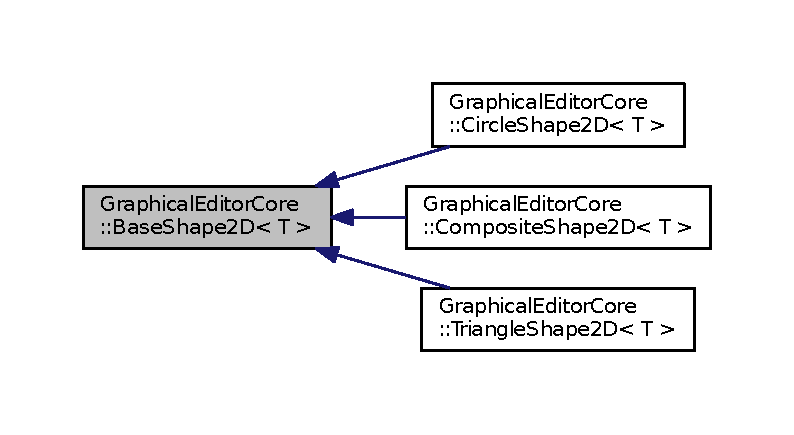
\includegraphics[width=350pt]{classGraphicalEditorCore_1_1BaseShape2D__inherit__graph}
\end{center}
\end{figure}
\subsection*{Public Member Functions}
\begin{DoxyCompactItemize}
\item 
\hyperlink{classGraphicalEditorCore_1_1BaseShape2D_a5d316bdae47e5b53ea6737f918a1340a}{Base\+Shape2D} (const size\+\_\+t \hyperlink{classGraphicalEditorCore_1_1BaseShape2D_ac66cfa23289ae36d70ff6b7c41dd791f}{id})
\item 
virtual \hyperlink{classGraphicalEditorCore_1_1BaseShape2D_ac3cf9262d27b9b1b84afc8ddb729f743}{$\sim$\+Base\+Shape2D} ()
\item 
virtual void \hyperlink{classGraphicalEditorCore_1_1BaseShape2D_a94a87b2fd8485cfb7d4ca97050d1bdde}{rotate} (const T clockwise\+\_\+angle)=0
\item 
virtual void \hyperlink{classGraphicalEditorCore_1_1BaseShape2D_adebef5c637da2c34a2fe728022740f94}{move\+Center} (const T dx, const T dy)=0
\item 
virtual void \hyperlink{classGraphicalEditorCore_1_1BaseShape2D_a9e6394ecf62e475a1d087e89258d4131}{move\+Vertex} (const T dx, const T dy, const size\+\_\+t index)=0
\item 
virtual void \hyperlink{classGraphicalEditorCore_1_1BaseShape2D_a2ff960ec57b180222a084642fa7dc780}{scale} (const T factor)=0
\item 
void \hyperlink{classGraphicalEditorCore_1_1BaseShape2D_abd6e21c5c3911a2926b210dd69584571}{reset\+Color\+Engine} (\hyperlink{classGraphicalEditorCore_1_1ColorEngineBase}{Color\+Engine\+Base} $\ast$)
\item 
const \hyperlink{classGraphicalEditorCore_1_1ColorEngineBase}{Color\+Engine\+Base} \& \hyperlink{classGraphicalEditorCore_1_1BaseShape2D_aed3e9da5f221282c0b7f958ad7c834c5}{color\+Engine} () const 
\item 
const size\+\_\+t \hyperlink{classGraphicalEditorCore_1_1BaseShape2D_ac66cfa23289ae36d70ff6b7c41dd791f}{id} () const noexcept
\item 
virtual void \hyperlink{classGraphicalEditorCore_1_1BaseShape2D_ab1db8da4296c0499c0e3bba4601bcc97}{debug\+\_\+print} ()
\item 
virtual void \hyperlink{classGraphicalEditorCore_1_1BaseShape2D_ac8f67c255fe72fd97aa7a5df80b698be}{append} (\hyperlink{classGraphicalEditorCore_1_1DocumentWriterBase}{Document\+Writer\+Base} \&) const 
\end{DoxyCompactItemize}


\subsection{Constructor \& Destructor Documentation}
\index{Graphical\+Editor\+Core\+::\+Base\+Shape2D@{Graphical\+Editor\+Core\+::\+Base\+Shape2D}!Base\+Shape2D@{Base\+Shape2D}}
\index{Base\+Shape2D@{Base\+Shape2D}!Graphical\+Editor\+Core\+::\+Base\+Shape2D@{Graphical\+Editor\+Core\+::\+Base\+Shape2D}}
\subsubsection[{\texorpdfstring{Base\+Shape2\+D(const size\+\_\+t id)}{BaseShape2D(const size_t id)}}]{\setlength{\rightskip}{0pt plus 5cm}template$<$typename T $>$ {\bf Graphical\+Editor\+Core\+::\+Base\+Shape2D}$<$ T $>$\+::{\bf Base\+Shape2D} (
\begin{DoxyParamCaption}
\item[{const size\+\_\+t}]{id}
\end{DoxyParamCaption}
)}\hypertarget{classGraphicalEditorCore_1_1BaseShape2D_a5d316bdae47e5b53ea6737f918a1340a}{}\label{classGraphicalEditorCore_1_1BaseShape2D_a5d316bdae47e5b53ea6737f918a1340a}
\index{Graphical\+Editor\+Core\+::\+Base\+Shape2D@{Graphical\+Editor\+Core\+::\+Base\+Shape2D}!````~Base\+Shape2D@{$\sim$\+Base\+Shape2D}}
\index{````~Base\+Shape2D@{$\sim$\+Base\+Shape2D}!Graphical\+Editor\+Core\+::\+Base\+Shape2D@{Graphical\+Editor\+Core\+::\+Base\+Shape2D}}
\subsubsection[{\texorpdfstring{$\sim$\+Base\+Shape2\+D()}{~BaseShape2D()}}]{\setlength{\rightskip}{0pt plus 5cm}template$<$typename T $>$ {\bf Graphical\+Editor\+Core\+::\+Base\+Shape2D}$<$ T $>$\+::$\sim${\bf Base\+Shape2D} (
\begin{DoxyParamCaption}
{}
\end{DoxyParamCaption}
)\hspace{0.3cm}{\ttfamily [virtual]}}\hypertarget{classGraphicalEditorCore_1_1BaseShape2D_ac3cf9262d27b9b1b84afc8ddb729f743}{}\label{classGraphicalEditorCore_1_1BaseShape2D_ac3cf9262d27b9b1b84afc8ddb729f743}


\subsection{Member Function Documentation}
\index{Graphical\+Editor\+Core\+::\+Base\+Shape2D@{Graphical\+Editor\+Core\+::\+Base\+Shape2D}!append@{append}}
\index{append@{append}!Graphical\+Editor\+Core\+::\+Base\+Shape2D@{Graphical\+Editor\+Core\+::\+Base\+Shape2D}}
\subsubsection[{\texorpdfstring{append(\+Document\+Writer\+Base \&) const }{append(DocumentWriterBase &) const }}]{\setlength{\rightskip}{0pt plus 5cm}template$<$typename T $>$ void {\bf Graphical\+Editor\+Core\+::\+Base\+Shape2D}$<$ T $>$\+::append (
\begin{DoxyParamCaption}
\item[{{\bf Document\+Writer\+Base} \&}]{wr\+\_\+eng}
\end{DoxyParamCaption}
) const\hspace{0.3cm}{\ttfamily [virtual]}}\hypertarget{classGraphicalEditorCore_1_1BaseShape2D_ac8f67c255fe72fd97aa7a5df80b698be}{}\label{classGraphicalEditorCore_1_1BaseShape2D_ac8f67c255fe72fd97aa7a5df80b698be}


Reimplemented in \hyperlink{classGraphicalEditorCore_1_1CompositeShape2D_af0ed12595f25239559d340c81d0fcb0d}{Graphical\+Editor\+Core\+::\+Composite\+Shape2\+D$<$ T $>$}, \hyperlink{classGraphicalEditorCore_1_1CircleShape2D_a56126680ab31d5b5de944b35e041855e}{Graphical\+Editor\+Core\+::\+Circle\+Shape2\+D$<$ T $>$}, and \hyperlink{classGraphicalEditorCore_1_1TriangleShape2D_af743a9e43c2f30d9b76dd4c37fe475c0}{Graphical\+Editor\+Core\+::\+Triangle\+Shape2\+D$<$ T $>$}.

\index{Graphical\+Editor\+Core\+::\+Base\+Shape2D@{Graphical\+Editor\+Core\+::\+Base\+Shape2D}!color\+Engine@{color\+Engine}}
\index{color\+Engine@{color\+Engine}!Graphical\+Editor\+Core\+::\+Base\+Shape2D@{Graphical\+Editor\+Core\+::\+Base\+Shape2D}}
\subsubsection[{\texorpdfstring{color\+Engine() const }{colorEngine() const }}]{\setlength{\rightskip}{0pt plus 5cm}template$<$typename T $>$ const {\bf Color\+Engine\+Base} \& {\bf Graphical\+Editor\+Core\+::\+Base\+Shape2D}$<$ T $>$\+::color\+Engine (
\begin{DoxyParamCaption}
{}
\end{DoxyParamCaption}
) const}\hypertarget{classGraphicalEditorCore_1_1BaseShape2D_aed3e9da5f221282c0b7f958ad7c834c5}{}\label{classGraphicalEditorCore_1_1BaseShape2D_aed3e9da5f221282c0b7f958ad7c834c5}
\index{Graphical\+Editor\+Core\+::\+Base\+Shape2D@{Graphical\+Editor\+Core\+::\+Base\+Shape2D}!debug\+\_\+print@{debug\+\_\+print}}
\index{debug\+\_\+print@{debug\+\_\+print}!Graphical\+Editor\+Core\+::\+Base\+Shape2D@{Graphical\+Editor\+Core\+::\+Base\+Shape2D}}
\subsubsection[{\texorpdfstring{debug\+\_\+print()}{debug_print()}}]{\setlength{\rightskip}{0pt plus 5cm}template$<$typename T $>$ void {\bf Graphical\+Editor\+Core\+::\+Base\+Shape2D}$<$ T $>$\+::debug\+\_\+print (
\begin{DoxyParamCaption}
{}
\end{DoxyParamCaption}
)\hspace{0.3cm}{\ttfamily [virtual]}}\hypertarget{classGraphicalEditorCore_1_1BaseShape2D_ab1db8da4296c0499c0e3bba4601bcc97}{}\label{classGraphicalEditorCore_1_1BaseShape2D_ab1db8da4296c0499c0e3bba4601bcc97}


Reimplemented in \hyperlink{classGraphicalEditorCore_1_1TriangleShape2D_a056f50df5a3891dba4c7ee46593ee5b4}{Graphical\+Editor\+Core\+::\+Triangle\+Shape2\+D$<$ T $>$}.

\index{Graphical\+Editor\+Core\+::\+Base\+Shape2D@{Graphical\+Editor\+Core\+::\+Base\+Shape2D}!id@{id}}
\index{id@{id}!Graphical\+Editor\+Core\+::\+Base\+Shape2D@{Graphical\+Editor\+Core\+::\+Base\+Shape2D}}
\subsubsection[{\texorpdfstring{id() const noexcept}{id() const noexcept}}]{\setlength{\rightskip}{0pt plus 5cm}template$<$typename T $>$ const size\+\_\+t {\bf Graphical\+Editor\+Core\+::\+Base\+Shape2D}$<$ T $>$\+::id (
\begin{DoxyParamCaption}
{}
\end{DoxyParamCaption}
) const\hspace{0.3cm}{\ttfamily [noexcept]}}\hypertarget{classGraphicalEditorCore_1_1BaseShape2D_ac66cfa23289ae36d70ff6b7c41dd791f}{}\label{classGraphicalEditorCore_1_1BaseShape2D_ac66cfa23289ae36d70ff6b7c41dd791f}
\index{Graphical\+Editor\+Core\+::\+Base\+Shape2D@{Graphical\+Editor\+Core\+::\+Base\+Shape2D}!move\+Center@{move\+Center}}
\index{move\+Center@{move\+Center}!Graphical\+Editor\+Core\+::\+Base\+Shape2D@{Graphical\+Editor\+Core\+::\+Base\+Shape2D}}
\subsubsection[{\texorpdfstring{move\+Center(const T dx, const T dy)=0}{moveCenter(const T dx, const T dy)=0}}]{\setlength{\rightskip}{0pt plus 5cm}template$<$typename T = double$>$ virtual void {\bf Graphical\+Editor\+Core\+::\+Base\+Shape2D}$<$ T $>$\+::move\+Center (
\begin{DoxyParamCaption}
\item[{const T}]{dx, }
\item[{const T}]{dy}
\end{DoxyParamCaption}
)\hspace{0.3cm}{\ttfamily [pure virtual]}}\hypertarget{classGraphicalEditorCore_1_1BaseShape2D_adebef5c637da2c34a2fe728022740f94}{}\label{classGraphicalEditorCore_1_1BaseShape2D_adebef5c637da2c34a2fe728022740f94}


Implemented in \hyperlink{classGraphicalEditorCore_1_1CompositeShape2D_a16cb9751cbd8f587f7f68ce831314e14}{Graphical\+Editor\+Core\+::\+Composite\+Shape2\+D$<$ T $>$}, \hyperlink{classGraphicalEditorCore_1_1CircleShape2D_a9bead68f8bd2224fe5e7a39d8e20f597}{Graphical\+Editor\+Core\+::\+Circle\+Shape2\+D$<$ T $>$}, and \hyperlink{classGraphicalEditorCore_1_1TriangleShape2D_a2b84784e80b932ef32641e7ac7d41bee}{Graphical\+Editor\+Core\+::\+Triangle\+Shape2\+D$<$ T $>$}.

\index{Graphical\+Editor\+Core\+::\+Base\+Shape2D@{Graphical\+Editor\+Core\+::\+Base\+Shape2D}!move\+Vertex@{move\+Vertex}}
\index{move\+Vertex@{move\+Vertex}!Graphical\+Editor\+Core\+::\+Base\+Shape2D@{Graphical\+Editor\+Core\+::\+Base\+Shape2D}}
\subsubsection[{\texorpdfstring{move\+Vertex(const T dx, const T dy, const size\+\_\+t index)=0}{moveVertex(const T dx, const T dy, const size_t index)=0}}]{\setlength{\rightskip}{0pt plus 5cm}template$<$typename T = double$>$ virtual void {\bf Graphical\+Editor\+Core\+::\+Base\+Shape2D}$<$ T $>$\+::move\+Vertex (
\begin{DoxyParamCaption}
\item[{const T}]{dx, }
\item[{const T}]{dy, }
\item[{const size\+\_\+t}]{index}
\end{DoxyParamCaption}
)\hspace{0.3cm}{\ttfamily [pure virtual]}}\hypertarget{classGraphicalEditorCore_1_1BaseShape2D_a9e6394ecf62e475a1d087e89258d4131}{}\label{classGraphicalEditorCore_1_1BaseShape2D_a9e6394ecf62e475a1d087e89258d4131}


Implemented in \hyperlink{classGraphicalEditorCore_1_1CompositeShape2D_a2754d592f39a2c442681fad8039e682f}{Graphical\+Editor\+Core\+::\+Composite\+Shape2\+D$<$ T $>$}, \hyperlink{classGraphicalEditorCore_1_1CircleShape2D_a833ad46ff3fd7e262238c332f50289e0}{Graphical\+Editor\+Core\+::\+Circle\+Shape2\+D$<$ T $>$}, and \hyperlink{classGraphicalEditorCore_1_1TriangleShape2D_a904d1d62d033013b636062c38df68d29}{Graphical\+Editor\+Core\+::\+Triangle\+Shape2\+D$<$ T $>$}.

\index{Graphical\+Editor\+Core\+::\+Base\+Shape2D@{Graphical\+Editor\+Core\+::\+Base\+Shape2D}!reset\+Color\+Engine@{reset\+Color\+Engine}}
\index{reset\+Color\+Engine@{reset\+Color\+Engine}!Graphical\+Editor\+Core\+::\+Base\+Shape2D@{Graphical\+Editor\+Core\+::\+Base\+Shape2D}}
\subsubsection[{\texorpdfstring{reset\+Color\+Engine(\+Color\+Engine\+Base $\ast$)}{resetColorEngine(ColorEngineBase *)}}]{\setlength{\rightskip}{0pt plus 5cm}template$<$typename T $>$ void {\bf Graphical\+Editor\+Core\+::\+Base\+Shape2D}$<$ T $>$\+::reset\+Color\+Engine (
\begin{DoxyParamCaption}
\item[{{\bf Color\+Engine\+Base} $\ast$}]{color\+\_\+engine}
\end{DoxyParamCaption}
)}\hypertarget{classGraphicalEditorCore_1_1BaseShape2D_abd6e21c5c3911a2926b210dd69584571}{}\label{classGraphicalEditorCore_1_1BaseShape2D_abd6e21c5c3911a2926b210dd69584571}
\index{Graphical\+Editor\+Core\+::\+Base\+Shape2D@{Graphical\+Editor\+Core\+::\+Base\+Shape2D}!rotate@{rotate}}
\index{rotate@{rotate}!Graphical\+Editor\+Core\+::\+Base\+Shape2D@{Graphical\+Editor\+Core\+::\+Base\+Shape2D}}
\subsubsection[{\texorpdfstring{rotate(const T clockwise\+\_\+angle)=0}{rotate(const T clockwise_angle)=0}}]{\setlength{\rightskip}{0pt plus 5cm}template$<$typename T = double$>$ virtual void {\bf Graphical\+Editor\+Core\+::\+Base\+Shape2D}$<$ T $>$\+::rotate (
\begin{DoxyParamCaption}
\item[{const T}]{clockwise\+\_\+angle}
\end{DoxyParamCaption}
)\hspace{0.3cm}{\ttfamily [pure virtual]}}\hypertarget{classGraphicalEditorCore_1_1BaseShape2D_a94a87b2fd8485cfb7d4ca97050d1bdde}{}\label{classGraphicalEditorCore_1_1BaseShape2D_a94a87b2fd8485cfb7d4ca97050d1bdde}


Implemented in \hyperlink{classGraphicalEditorCore_1_1CompositeShape2D_a1ad124ab5448a4276d06742318744473}{Graphical\+Editor\+Core\+::\+Composite\+Shape2\+D$<$ T $>$}, \hyperlink{classGraphicalEditorCore_1_1CircleShape2D_a587709b51a3b79c915c4939c65be178c}{Graphical\+Editor\+Core\+::\+Circle\+Shape2\+D$<$ T $>$}, and \hyperlink{classGraphicalEditorCore_1_1TriangleShape2D_a70baf8d77cdaa6107cac5ba2c8f9bc5b}{Graphical\+Editor\+Core\+::\+Triangle\+Shape2\+D$<$ T $>$}.

\index{Graphical\+Editor\+Core\+::\+Base\+Shape2D@{Graphical\+Editor\+Core\+::\+Base\+Shape2D}!scale@{scale}}
\index{scale@{scale}!Graphical\+Editor\+Core\+::\+Base\+Shape2D@{Graphical\+Editor\+Core\+::\+Base\+Shape2D}}
\subsubsection[{\texorpdfstring{scale(const T factor)=0}{scale(const T factor)=0}}]{\setlength{\rightskip}{0pt plus 5cm}template$<$typename T = double$>$ virtual void {\bf Graphical\+Editor\+Core\+::\+Base\+Shape2D}$<$ T $>$\+::scale (
\begin{DoxyParamCaption}
\item[{const T}]{factor}
\end{DoxyParamCaption}
)\hspace{0.3cm}{\ttfamily [pure virtual]}}\hypertarget{classGraphicalEditorCore_1_1BaseShape2D_a2ff960ec57b180222a084642fa7dc780}{}\label{classGraphicalEditorCore_1_1BaseShape2D_a2ff960ec57b180222a084642fa7dc780}


Implemented in \hyperlink{classGraphicalEditorCore_1_1CompositeShape2D_ae1d0a3270ae8eeec8a87c5a37d657336}{Graphical\+Editor\+Core\+::\+Composite\+Shape2\+D$<$ T $>$}, \hyperlink{classGraphicalEditorCore_1_1CircleShape2D_aac68ae27380865c53a7a5e20b124725b}{Graphical\+Editor\+Core\+::\+Circle\+Shape2\+D$<$ T $>$}, and \hyperlink{classGraphicalEditorCore_1_1TriangleShape2D_a769d7053c7410e288abeaa8e6122ee26}{Graphical\+Editor\+Core\+::\+Triangle\+Shape2\+D$<$ T $>$}.



The documentation for this class was generated from the following files\+:\begin{DoxyCompactItemize}
\item 
05\+\_\+editor/\hyperlink{shapes__2d_8h}{shapes\+\_\+2d.\+h}\item 
05\+\_\+editor/\hyperlink{base__shape__2d_8cpp}{base\+\_\+shape\+\_\+2d.\+cpp}\end{DoxyCompactItemize}

\hypertarget{classCellObserver}{}\section{Cell\+Observer$<$ T, Default\+Value $>$ Class Template Reference}
\label{classCellObserver}\index{Cell\+Observer$<$ T, Default\+Value $>$@{Cell\+Observer$<$ T, Default\+Value $>$}}


{\ttfamily \#include $<$cell\+\_\+observer.\+h$>$}

\subsection*{Public Member Functions}
\begin{DoxyCompactItemize}
\item 
\hyperlink{classCellObserver_a04a245848c8cd86cfc471b0f278dc546}{Cell\+Observer} ()
\item 
\hyperlink{classCellObserver_a4a930e2b7ac95c7c11f34cee6f868bc1}{$\sim$\+Cell\+Observer} ()=default
\item 
void \hyperlink{classCellObserver_a5838eda25127346a5a296c38a651f764}{set\+\_\+index} (const size\+\_\+t index)
\item 
void \hyperlink{classCellObserver_aa94b7933d2e0a3e576f6ab35c061bcfa}{bind} (\hyperlink{classInfiniteRow}{Infinite\+Row}$<$ T, Default\+Value $>$ $\ast$const host\+\_\+row)
\item 
\hyperlink{classCellObserver}{Cell\+Observer} \& \hyperlink{classCellObserver_a51d022b73fee930b38516437f8bd0b49}{operator=} (const T \&rhs\+\_\+value)
\end{DoxyCompactItemize}


\subsection{Constructor \& Destructor Documentation}
\index{Cell\+Observer@{Cell\+Observer}!Cell\+Observer@{Cell\+Observer}}
\index{Cell\+Observer@{Cell\+Observer}!Cell\+Observer@{Cell\+Observer}}
\subsubsection[{\texorpdfstring{Cell\+Observer()}{CellObserver()}}]{\setlength{\rightskip}{0pt plus 5cm}template$<$typename T , T Default\+Value$>$ {\bf Cell\+Observer}$<$ T, Default\+Value $>$\+::{\bf Cell\+Observer} (
\begin{DoxyParamCaption}
{}
\end{DoxyParamCaption}
)}\hypertarget{classCellObserver_a04a245848c8cd86cfc471b0f278dc546}{}\label{classCellObserver_a04a245848c8cd86cfc471b0f278dc546}
\index{Cell\+Observer@{Cell\+Observer}!````~Cell\+Observer@{$\sim$\+Cell\+Observer}}
\index{````~Cell\+Observer@{$\sim$\+Cell\+Observer}!Cell\+Observer@{Cell\+Observer}}
\subsubsection[{\texorpdfstring{$\sim$\+Cell\+Observer()=default}{~CellObserver()=default}}]{\setlength{\rightskip}{0pt plus 5cm}template$<$typename T, T Default\+Value$>$ {\bf Cell\+Observer}$<$ T, Default\+Value $>$\+::$\sim${\bf Cell\+Observer} (
\begin{DoxyParamCaption}
{}
\end{DoxyParamCaption}
)\hspace{0.3cm}{\ttfamily [default]}}\hypertarget{classCellObserver_a4a930e2b7ac95c7c11f34cee6f868bc1}{}\label{classCellObserver_a4a930e2b7ac95c7c11f34cee6f868bc1}


\subsection{Member Function Documentation}
\index{Cell\+Observer@{Cell\+Observer}!bind@{bind}}
\index{bind@{bind}!Cell\+Observer@{Cell\+Observer}}
\subsubsection[{\texorpdfstring{bind(\+Infinite\+Row$<$ T, Default\+Value $>$ $\ast$const host\+\_\+row)}{bind(InfiniteRow< T, DefaultValue > *const host_row)}}]{\setlength{\rightskip}{0pt plus 5cm}template$<$typename T , T Default\+Value$>$ void {\bf Cell\+Observer}$<$ T, Default\+Value $>$\+::bind (
\begin{DoxyParamCaption}
\item[{{\bf Infinite\+Row}$<$ T, Default\+Value $>$ $\ast$const}]{host\+\_\+row}
\end{DoxyParamCaption}
)}\hypertarget{classCellObserver_aa94b7933d2e0a3e576f6ab35c061bcfa}{}\label{classCellObserver_aa94b7933d2e0a3e576f6ab35c061bcfa}
\index{Cell\+Observer@{Cell\+Observer}!operator=@{operator=}}
\index{operator=@{operator=}!Cell\+Observer@{Cell\+Observer}}
\subsubsection[{\texorpdfstring{operator=(const T \&rhs\+\_\+value)}{operator=(const T &rhs_value)}}]{\setlength{\rightskip}{0pt plus 5cm}template$<$typename T , T Default\+Value$>$ {\bf Cell\+Observer}$<$ T, Default\+Value $>$ \& {\bf Cell\+Observer}$<$ T, Default\+Value $>$\+::operator= (
\begin{DoxyParamCaption}
\item[{const T \&}]{rhs\+\_\+value}
\end{DoxyParamCaption}
)}\hypertarget{classCellObserver_a51d022b73fee930b38516437f8bd0b49}{}\label{classCellObserver_a51d022b73fee930b38516437f8bd0b49}
Operator is used for cells assignment\+: it calls update value of row if and only if it does not coincide with the default value. \index{Cell\+Observer@{Cell\+Observer}!set\+\_\+index@{set\+\_\+index}}
\index{set\+\_\+index@{set\+\_\+index}!Cell\+Observer@{Cell\+Observer}}
\subsubsection[{\texorpdfstring{set\+\_\+index(const size\+\_\+t index)}{set_index(const size_t index)}}]{\setlength{\rightskip}{0pt plus 5cm}template$<$typename T , T Default\+Value$>$ void {\bf Cell\+Observer}$<$ T, Default\+Value $>$\+::set\+\_\+index (
\begin{DoxyParamCaption}
\item[{const size\+\_\+t}]{index}
\end{DoxyParamCaption}
)}\hypertarget{classCellObserver_a5838eda25127346a5a296c38a651f764}{}\label{classCellObserver_a5838eda25127346a5a296c38a651f764}


The documentation for this class was generated from the following files\+:\begin{DoxyCompactItemize}
\item 
06\+\_\+matrix/\hyperlink{cell__observer_8h}{cell\+\_\+observer.\+h}\item 
06\+\_\+matrix/\hyperlink{cell__observer_8cpp}{cell\+\_\+observer.\+cpp}\end{DoxyCompactItemize}

\hypertarget{classGraphicalEditorCore_1_1CircleShape2D}{}\section{Graphical\+Editor\+Core\+:\+:Circle\+Shape2D$<$ T $>$ Class Template Reference}
\label{classGraphicalEditorCore_1_1CircleShape2D}\index{Graphical\+Editor\+Core\+::\+Circle\+Shape2\+D$<$ T $>$@{Graphical\+Editor\+Core\+::\+Circle\+Shape2\+D$<$ T $>$}}


{\ttfamily \#include $<$shapes\+\_\+2d.\+h$>$}



Inheritance diagram for Graphical\+Editor\+Core\+:\+:Circle\+Shape2D$<$ T $>$\+:
\nopagebreak
\begin{figure}[H]
\begin{center}
\leavevmode
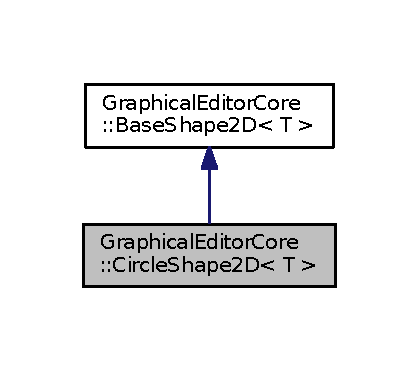
\includegraphics[width=201pt]{classGraphicalEditorCore_1_1CircleShape2D__inherit__graph}
\end{center}
\end{figure}


Collaboration diagram for Graphical\+Editor\+Core\+:\+:Circle\+Shape2D$<$ T $>$\+:
\nopagebreak
\begin{figure}[H]
\begin{center}
\leavevmode
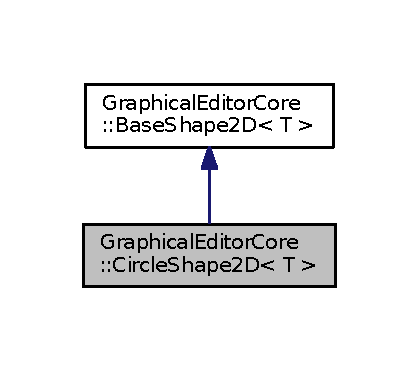
\includegraphics[width=201pt]{classGraphicalEditorCore_1_1CircleShape2D__coll__graph}
\end{center}
\end{figure}
\subsection*{Public Member Functions}
\begin{DoxyCompactItemize}
\item 
\hyperlink{classGraphicalEditorCore_1_1CircleShape2D_ac6e40c6596bafc87cb948f61225955e2}{Circle\+Shape2D} (const size\+\_\+t \hyperlink{classGraphicalEditorCore_1_1BaseShape2D_ac66cfa23289ae36d70ff6b7c41dd791f}{id})
\item 
virtual \hyperlink{classGraphicalEditorCore_1_1CircleShape2D_a8dac5c648f62af0e23fa50442d14407b}{$\sim$\+Circle\+Shape2D} ()
\item 
virtual void \hyperlink{classGraphicalEditorCore_1_1CircleShape2D_a587709b51a3b79c915c4939c65be178c}{rotate} (const T clockwise\+\_\+angle) override
\item 
virtual void \hyperlink{classGraphicalEditorCore_1_1CircleShape2D_a9bead68f8bd2224fe5e7a39d8e20f597}{move\+Center} (const T dx, const T dy) override
\item 
virtual void \hyperlink{classGraphicalEditorCore_1_1CircleShape2D_a833ad46ff3fd7e262238c332f50289e0}{move\+Vertex} (const T dx, const T dy, const size\+\_\+t index) override
\item 
virtual void \hyperlink{classGraphicalEditorCore_1_1CircleShape2D_aac68ae27380865c53a7a5e20b124725b}{scale} (const T factor) override
\end{DoxyCompactItemize}


\subsection{Constructor \& Destructor Documentation}
\index{Graphical\+Editor\+Core\+::\+Circle\+Shape2D@{Graphical\+Editor\+Core\+::\+Circle\+Shape2D}!Circle\+Shape2D@{Circle\+Shape2D}}
\index{Circle\+Shape2D@{Circle\+Shape2D}!Graphical\+Editor\+Core\+::\+Circle\+Shape2D@{Graphical\+Editor\+Core\+::\+Circle\+Shape2D}}
\subsubsection[{\texorpdfstring{Circle\+Shape2\+D(const size\+\_\+t id)}{CircleShape2D(const size_t id)}}]{\setlength{\rightskip}{0pt plus 5cm}template$<$typename T $>$ {\bf Graphical\+Editor\+Core\+::\+Circle\+Shape2D}$<$ T $>$\+::{\bf Circle\+Shape2D} (
\begin{DoxyParamCaption}
\item[{const size\+\_\+t}]{id}
\end{DoxyParamCaption}
)}\hypertarget{classGraphicalEditorCore_1_1CircleShape2D_ac6e40c6596bafc87cb948f61225955e2}{}\label{classGraphicalEditorCore_1_1CircleShape2D_ac6e40c6596bafc87cb948f61225955e2}
\index{Graphical\+Editor\+Core\+::\+Circle\+Shape2D@{Graphical\+Editor\+Core\+::\+Circle\+Shape2D}!````~Circle\+Shape2D@{$\sim$\+Circle\+Shape2D}}
\index{````~Circle\+Shape2D@{$\sim$\+Circle\+Shape2D}!Graphical\+Editor\+Core\+::\+Circle\+Shape2D@{Graphical\+Editor\+Core\+::\+Circle\+Shape2D}}
\subsubsection[{\texorpdfstring{$\sim$\+Circle\+Shape2\+D()}{~CircleShape2D()}}]{\setlength{\rightskip}{0pt plus 5cm}template$<$typename T $>$ {\bf Graphical\+Editor\+Core\+::\+Circle\+Shape2D}$<$ T $>$\+::$\sim${\bf Circle\+Shape2D} (
\begin{DoxyParamCaption}
{}
\end{DoxyParamCaption}
)\hspace{0.3cm}{\ttfamily [virtual]}}\hypertarget{classGraphicalEditorCore_1_1CircleShape2D_a8dac5c648f62af0e23fa50442d14407b}{}\label{classGraphicalEditorCore_1_1CircleShape2D_a8dac5c648f62af0e23fa50442d14407b}


\subsection{Member Function Documentation}
\index{Graphical\+Editor\+Core\+::\+Circle\+Shape2D@{Graphical\+Editor\+Core\+::\+Circle\+Shape2D}!move\+Center@{move\+Center}}
\index{move\+Center@{move\+Center}!Graphical\+Editor\+Core\+::\+Circle\+Shape2D@{Graphical\+Editor\+Core\+::\+Circle\+Shape2D}}
\subsubsection[{\texorpdfstring{move\+Center(const T dx, const T dy) override}{moveCenter(const T dx, const T dy) override}}]{\setlength{\rightskip}{0pt plus 5cm}template$<$typename T $>$ void {\bf Graphical\+Editor\+Core\+::\+Circle\+Shape2D}$<$ T $>$\+::move\+Center (
\begin{DoxyParamCaption}
\item[{const T}]{dx, }
\item[{const T}]{dy}
\end{DoxyParamCaption}
)\hspace{0.3cm}{\ttfamily [override]}, {\ttfamily [virtual]}}\hypertarget{classGraphicalEditorCore_1_1CircleShape2D_a9bead68f8bd2224fe5e7a39d8e20f597}{}\label{classGraphicalEditorCore_1_1CircleShape2D_a9bead68f8bd2224fe5e7a39d8e20f597}


Implements \hyperlink{classGraphicalEditorCore_1_1BaseShape2D_adebef5c637da2c34a2fe728022740f94}{Graphical\+Editor\+Core\+::\+Base\+Shape2\+D$<$ T $>$}.

\index{Graphical\+Editor\+Core\+::\+Circle\+Shape2D@{Graphical\+Editor\+Core\+::\+Circle\+Shape2D}!move\+Vertex@{move\+Vertex}}
\index{move\+Vertex@{move\+Vertex}!Graphical\+Editor\+Core\+::\+Circle\+Shape2D@{Graphical\+Editor\+Core\+::\+Circle\+Shape2D}}
\subsubsection[{\texorpdfstring{move\+Vertex(const T dx, const T dy, const size\+\_\+t index) override}{moveVertex(const T dx, const T dy, const size_t index) override}}]{\setlength{\rightskip}{0pt plus 5cm}template$<$typename T $>$ void {\bf Graphical\+Editor\+Core\+::\+Circle\+Shape2D}$<$ T $>$\+::move\+Vertex (
\begin{DoxyParamCaption}
\item[{const T}]{dx, }
\item[{const T}]{dy, }
\item[{const size\+\_\+t}]{index}
\end{DoxyParamCaption}
)\hspace{0.3cm}{\ttfamily [override]}, {\ttfamily [virtual]}}\hypertarget{classGraphicalEditorCore_1_1CircleShape2D_a833ad46ff3fd7e262238c332f50289e0}{}\label{classGraphicalEditorCore_1_1CircleShape2D_a833ad46ff3fd7e262238c332f50289e0}


Implements \hyperlink{classGraphicalEditorCore_1_1BaseShape2D_a9e6394ecf62e475a1d087e89258d4131}{Graphical\+Editor\+Core\+::\+Base\+Shape2\+D$<$ T $>$}.

\index{Graphical\+Editor\+Core\+::\+Circle\+Shape2D@{Graphical\+Editor\+Core\+::\+Circle\+Shape2D}!rotate@{rotate}}
\index{rotate@{rotate}!Graphical\+Editor\+Core\+::\+Circle\+Shape2D@{Graphical\+Editor\+Core\+::\+Circle\+Shape2D}}
\subsubsection[{\texorpdfstring{rotate(const T clockwise\+\_\+angle) override}{rotate(const T clockwise_angle) override}}]{\setlength{\rightskip}{0pt plus 5cm}template$<$typename T $>$ void {\bf Graphical\+Editor\+Core\+::\+Circle\+Shape2D}$<$ T $>$\+::rotate (
\begin{DoxyParamCaption}
\item[{const T}]{clockwise\+\_\+angle}
\end{DoxyParamCaption}
)\hspace{0.3cm}{\ttfamily [override]}, {\ttfamily [virtual]}}\hypertarget{classGraphicalEditorCore_1_1CircleShape2D_a587709b51a3b79c915c4939c65be178c}{}\label{classGraphicalEditorCore_1_1CircleShape2D_a587709b51a3b79c915c4939c65be178c}


Implements \hyperlink{classGraphicalEditorCore_1_1BaseShape2D_a94a87b2fd8485cfb7d4ca97050d1bdde}{Graphical\+Editor\+Core\+::\+Base\+Shape2\+D$<$ T $>$}.

\index{Graphical\+Editor\+Core\+::\+Circle\+Shape2D@{Graphical\+Editor\+Core\+::\+Circle\+Shape2D}!scale@{scale}}
\index{scale@{scale}!Graphical\+Editor\+Core\+::\+Circle\+Shape2D@{Graphical\+Editor\+Core\+::\+Circle\+Shape2D}}
\subsubsection[{\texorpdfstring{scale(const T factor) override}{scale(const T factor) override}}]{\setlength{\rightskip}{0pt plus 5cm}template$<$typename T $>$ void {\bf Graphical\+Editor\+Core\+::\+Circle\+Shape2D}$<$ T $>$\+::scale (
\begin{DoxyParamCaption}
\item[{const T}]{factor}
\end{DoxyParamCaption}
)\hspace{0.3cm}{\ttfamily [override]}, {\ttfamily [virtual]}}\hypertarget{classGraphicalEditorCore_1_1CircleShape2D_aac68ae27380865c53a7a5e20b124725b}{}\label{classGraphicalEditorCore_1_1CircleShape2D_aac68ae27380865c53a7a5e20b124725b}


Implements \hyperlink{classGraphicalEditorCore_1_1BaseShape2D_a2ff960ec57b180222a084642fa7dc780}{Graphical\+Editor\+Core\+::\+Base\+Shape2\+D$<$ T $>$}.



The documentation for this class was generated from the following files\+:\begin{DoxyCompactItemize}
\item 
05\+\_\+editor/\hyperlink{shapes__2d_8h}{shapes\+\_\+2d.\+h}\item 
05\+\_\+editor/\hyperlink{circle__shape__2d_8cpp}{circle\+\_\+shape\+\_\+2d.\+cpp}\end{DoxyCompactItemize}

\hypertarget{structGraphicalEditorCore_1_1color__index}{}\section{Graphical\+Editor\+Core\+:\+:color\+\_\+index$<$ Rgb\+Color $>$ Struct Template Reference}
\label{structGraphicalEditorCore_1_1color__index}\index{Graphical\+Editor\+Core\+::color\+\_\+index$<$ Rgb\+Color $>$@{Graphical\+Editor\+Core\+::color\+\_\+index$<$ Rgb\+Color $>$}}


{\ttfamily \#include $<$color\+\_\+engine.\+h$>$}



The documentation for this struct was generated from the following file\+:\begin{DoxyCompactItemize}
\item 
05\+\_\+editor/\hyperlink{color__engine_8h}{color\+\_\+engine.\+h}\end{DoxyCompactItemize}

\hypertarget{structGraphicalEditorCore_1_1color__index_3_01RgbColor_1_1Blue_01_4}{}\section{Graphical\+Editor\+Core\+:\+:color\+\_\+index$<$ Rgb\+Color\+:\+:Blue $>$ Struct Template Reference}
\label{structGraphicalEditorCore_1_1color__index_3_01RgbColor_1_1Blue_01_4}\index{Graphical\+Editor\+Core\+::color\+\_\+index$<$ Rgb\+Color\+::\+Blue $>$@{Graphical\+Editor\+Core\+::color\+\_\+index$<$ Rgb\+Color\+::\+Blue $>$}}


{\ttfamily \#include $<$color\+\_\+engine.\+h$>$}

\subsection*{Static Public Member Functions}
\begin{DoxyCompactItemize}
\item 
static constexpr uint8\+\_\+t \hyperlink{structGraphicalEditorCore_1_1color__index_3_01RgbColor_1_1Blue_01_4_ab88fc39fae9e5fa42840fcc967d43041}{value} ()
\end{DoxyCompactItemize}


\subsection{Member Function Documentation}
\index{Graphical\+Editor\+Core\+::color\+\_\+index$<$ Rgb\+Color\+::\+Blue $>$@{Graphical\+Editor\+Core\+::color\+\_\+index$<$ Rgb\+Color\+::\+Blue $>$}!value@{value}}
\index{value@{value}!Graphical\+Editor\+Core\+::color\+\_\+index$<$ Rgb\+Color\+::\+Blue $>$@{Graphical\+Editor\+Core\+::color\+\_\+index$<$ Rgb\+Color\+::\+Blue $>$}}
\subsubsection[{\texorpdfstring{value()}{value()}}]{\setlength{\rightskip}{0pt plus 5cm}constexpr uint8\+\_\+t {\bf Graphical\+Editor\+Core\+::color\+\_\+index}$<$ {\bf Rgb\+Color\+::\+Blue} $>$\+::value (
\begin{DoxyParamCaption}
{}
\end{DoxyParamCaption}
)\hspace{0.3cm}{\ttfamily [static]}}\hypertarget{structGraphicalEditorCore_1_1color__index_3_01RgbColor_1_1Blue_01_4_ab88fc39fae9e5fa42840fcc967d43041}{}\label{structGraphicalEditorCore_1_1color__index_3_01RgbColor_1_1Blue_01_4_ab88fc39fae9e5fa42840fcc967d43041}


The documentation for this struct was generated from the following files\+:\begin{DoxyCompactItemize}
\item 
05\+\_\+editor/\hyperlink{color__engine_8h}{color\+\_\+engine.\+h}\item 
05\+\_\+editor/\hyperlink{color__engine_8cpp}{color\+\_\+engine.\+cpp}\end{DoxyCompactItemize}

\hypertarget{structGraphicalEditorCore_1_1color__index_3_01RgbColor_1_1Green_01_4}{}\section{Graphical\+Editor\+Core\+:\+:color\+\_\+index$<$ Rgb\+Color\+:\+:Green $>$ Struct Template Reference}
\label{structGraphicalEditorCore_1_1color__index_3_01RgbColor_1_1Green_01_4}\index{Graphical\+Editor\+Core\+::color\+\_\+index$<$ Rgb\+Color\+::\+Green $>$@{Graphical\+Editor\+Core\+::color\+\_\+index$<$ Rgb\+Color\+::\+Green $>$}}


{\ttfamily \#include $<$color\+\_\+engine.\+h$>$}

\subsection*{Static Public Member Functions}
\begin{DoxyCompactItemize}
\item 
static constexpr uint8\+\_\+t \hyperlink{structGraphicalEditorCore_1_1color__index_3_01RgbColor_1_1Green_01_4_aaf9a0203b8f6e8925dbaf5ef225d3ef2}{value} ()
\end{DoxyCompactItemize}


\subsection{Member Function Documentation}
\index{Graphical\+Editor\+Core\+::color\+\_\+index$<$ Rgb\+Color\+::\+Green $>$@{Graphical\+Editor\+Core\+::color\+\_\+index$<$ Rgb\+Color\+::\+Green $>$}!value@{value}}
\index{value@{value}!Graphical\+Editor\+Core\+::color\+\_\+index$<$ Rgb\+Color\+::\+Green $>$@{Graphical\+Editor\+Core\+::color\+\_\+index$<$ Rgb\+Color\+::\+Green $>$}}
\subsubsection[{\texorpdfstring{value()}{value()}}]{\setlength{\rightskip}{0pt plus 5cm}constexpr uint8\+\_\+t {\bf Graphical\+Editor\+Core\+::color\+\_\+index}$<$ {\bf Rgb\+Color\+::\+Green} $>$\+::value (
\begin{DoxyParamCaption}
{}
\end{DoxyParamCaption}
)\hspace{0.3cm}{\ttfamily [static]}}\hypertarget{structGraphicalEditorCore_1_1color__index_3_01RgbColor_1_1Green_01_4_aaf9a0203b8f6e8925dbaf5ef225d3ef2}{}\label{structGraphicalEditorCore_1_1color__index_3_01RgbColor_1_1Green_01_4_aaf9a0203b8f6e8925dbaf5ef225d3ef2}


The documentation for this struct was generated from the following files\+:\begin{DoxyCompactItemize}
\item 
05\+\_\+editor/\hyperlink{color__engine_8h}{color\+\_\+engine.\+h}\item 
05\+\_\+editor/\hyperlink{color__engine_8cpp}{color\+\_\+engine.\+cpp}\end{DoxyCompactItemize}

\hypertarget{structGraphicalEditorCore_1_1color__index_3_01RgbColor_1_1Red_01_4}{}\section{Graphical\+Editor\+Core\+:\+:color\+\_\+index$<$ Rgb\+Color\+:\+:Red $>$ Struct Template Reference}
\label{structGraphicalEditorCore_1_1color__index_3_01RgbColor_1_1Red_01_4}\index{Graphical\+Editor\+Core\+::color\+\_\+index$<$ Rgb\+Color\+::\+Red $>$@{Graphical\+Editor\+Core\+::color\+\_\+index$<$ Rgb\+Color\+::\+Red $>$}}


{\ttfamily \#include $<$color\+\_\+engine.\+h$>$}

\subsection*{Static Public Member Functions}
\begin{DoxyCompactItemize}
\item 
static constexpr uint8\+\_\+t \hyperlink{structGraphicalEditorCore_1_1color__index_3_01RgbColor_1_1Red_01_4_a8cc20564551ec4cd014595d69b2c3926}{value} ()
\end{DoxyCompactItemize}


\subsection{Member Function Documentation}
\index{Graphical\+Editor\+Core\+::color\+\_\+index$<$ Rgb\+Color\+::\+Red $>$@{Graphical\+Editor\+Core\+::color\+\_\+index$<$ Rgb\+Color\+::\+Red $>$}!value@{value}}
\index{value@{value}!Graphical\+Editor\+Core\+::color\+\_\+index$<$ Rgb\+Color\+::\+Red $>$@{Graphical\+Editor\+Core\+::color\+\_\+index$<$ Rgb\+Color\+::\+Red $>$}}
\subsubsection[{\texorpdfstring{value()}{value()}}]{\setlength{\rightskip}{0pt plus 5cm}constexpr uint8\+\_\+t {\bf Graphical\+Editor\+Core\+::color\+\_\+index}$<$ {\bf Rgb\+Color\+::\+Red} $>$\+::value (
\begin{DoxyParamCaption}
{}
\end{DoxyParamCaption}
)\hspace{0.3cm}{\ttfamily [static]}}\hypertarget{structGraphicalEditorCore_1_1color__index_3_01RgbColor_1_1Red_01_4_a8cc20564551ec4cd014595d69b2c3926}{}\label{structGraphicalEditorCore_1_1color__index_3_01RgbColor_1_1Red_01_4_a8cc20564551ec4cd014595d69b2c3926}


The documentation for this struct was generated from the following files\+:\begin{DoxyCompactItemize}
\item 
05\+\_\+editor/\hyperlink{color__engine_8h}{color\+\_\+engine.\+h}\item 
05\+\_\+editor/\hyperlink{color__engine_8cpp}{color\+\_\+engine.\+cpp}\end{DoxyCompactItemize}

\hypertarget{classGraphicalEditorCore_1_1ColorEngineBase}{}\section{Graphical\+Editor\+Core\+:\+:Color\+Engine\+Base Class Reference}
\label{classGraphicalEditorCore_1_1ColorEngineBase}\index{Graphical\+Editor\+Core\+::\+Color\+Engine\+Base@{Graphical\+Editor\+Core\+::\+Color\+Engine\+Base}}


{\ttfamily \#include $<$color\+\_\+engine.\+h$>$}



Inheritance diagram for Graphical\+Editor\+Core\+:\+:Color\+Engine\+Base\+:
\nopagebreak
\begin{figure}[H]
\begin{center}
\leavevmode
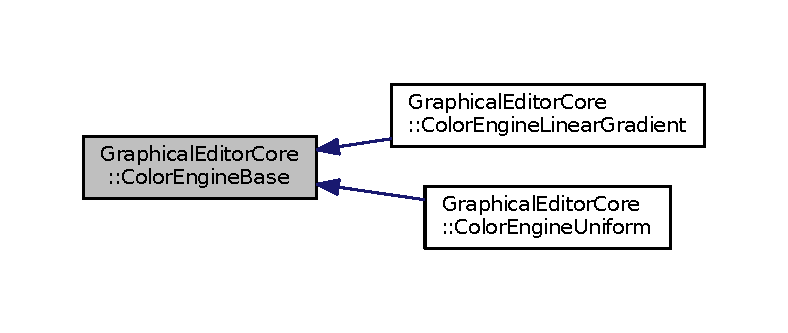
\includegraphics[width=350pt]{classGraphicalEditorCore_1_1ColorEngineBase__inherit__graph}
\end{center}
\end{figure}
\subsection*{Public Member Functions}
\begin{DoxyCompactItemize}
\item 
\hyperlink{classGraphicalEditorCore_1_1ColorEngineBase_ae9aaf24b0d10206078560352af041058}{Color\+Engine\+Base} ()=default
\item 
virtual \hyperlink{classGraphicalEditorCore_1_1ColorEngineBase_a286d4bf617e3cfa67084e436020cd722}{$\sim$\+Color\+Engine\+Base} ()=default
\item 
\hyperlink{classGraphicalEditorCore_1_1ColorEngineBase_ac101595bae8f49c09446064c47e0c628}{Color\+Engine\+Base} (const \hyperlink{classGraphicalEditorCore_1_1ColorEngineBase}{Color\+Engine\+Base} \&)=default
\item 
\hyperlink{classGraphicalEditorCore_1_1ColorEngineBase_a55df45f8e28e519452b9185ea3c5856d}{Color\+Engine\+Base} (\hyperlink{classGraphicalEditorCore_1_1ColorEngineBase}{Color\+Engine\+Base} \&\&)=default
\item 
\hyperlink{classGraphicalEditorCore_1_1ColorEngineBase}{Color\+Engine\+Base} \& \hyperlink{classGraphicalEditorCore_1_1ColorEngineBase_ac0c10c370c1881f9849969e1a9cbb2c1}{operator=} (const \hyperlink{classGraphicalEditorCore_1_1ColorEngineBase}{Color\+Engine\+Base} \&)=default
\item 
\hyperlink{classGraphicalEditorCore_1_1ColorEngineBase}{Color\+Engine\+Base} \& \hyperlink{classGraphicalEditorCore_1_1ColorEngineBase_a5b9a13ca99cde927d921a78fd00b0fc9}{operator=} (\hyperlink{classGraphicalEditorCore_1_1ColorEngineBase}{Color\+Engine\+Base} \&\&)=default
\item 
virtual uint8\+\_\+t \hyperlink{classGraphicalEditorCore_1_1ColorEngineBase_a9d0b1a48ea117d8f47c43b9c63982dc5}{red} (const size\+\_\+t i\+\_\+x, const size\+\_\+t j\+\_\+y) const =0
\item 
virtual uint8\+\_\+t \hyperlink{classGraphicalEditorCore_1_1ColorEngineBase_a748837e34f2bf4409ae36a5d9ea02e27}{green} (const size\+\_\+t i\+\_\+x, const size\+\_\+t j\+\_\+y) const =0
\item 
virtual uint8\+\_\+t \hyperlink{classGraphicalEditorCore_1_1ColorEngineBase_a86a1c186366f3df9469e36421167f8cb}{blue} (const size\+\_\+t i\+\_\+x, const size\+\_\+t j\+\_\+y) const =0
\end{DoxyCompactItemize}


\subsection{Constructor \& Destructor Documentation}
\index{Graphical\+Editor\+Core\+::\+Color\+Engine\+Base@{Graphical\+Editor\+Core\+::\+Color\+Engine\+Base}!Color\+Engine\+Base@{Color\+Engine\+Base}}
\index{Color\+Engine\+Base@{Color\+Engine\+Base}!Graphical\+Editor\+Core\+::\+Color\+Engine\+Base@{Graphical\+Editor\+Core\+::\+Color\+Engine\+Base}}
\subsubsection[{\texorpdfstring{Color\+Engine\+Base()=default}{ColorEngineBase()=default}}]{\setlength{\rightskip}{0pt plus 5cm}Graphical\+Editor\+Core\+::\+Color\+Engine\+Base\+::\+Color\+Engine\+Base (
\begin{DoxyParamCaption}
{}
\end{DoxyParamCaption}
)\hspace{0.3cm}{\ttfamily [default]}}\hypertarget{classGraphicalEditorCore_1_1ColorEngineBase_ae9aaf24b0d10206078560352af041058}{}\label{classGraphicalEditorCore_1_1ColorEngineBase_ae9aaf24b0d10206078560352af041058}
\index{Graphical\+Editor\+Core\+::\+Color\+Engine\+Base@{Graphical\+Editor\+Core\+::\+Color\+Engine\+Base}!````~Color\+Engine\+Base@{$\sim$\+Color\+Engine\+Base}}
\index{````~Color\+Engine\+Base@{$\sim$\+Color\+Engine\+Base}!Graphical\+Editor\+Core\+::\+Color\+Engine\+Base@{Graphical\+Editor\+Core\+::\+Color\+Engine\+Base}}
\subsubsection[{\texorpdfstring{$\sim$\+Color\+Engine\+Base()=default}{~ColorEngineBase()=default}}]{\setlength{\rightskip}{0pt plus 5cm}virtual Graphical\+Editor\+Core\+::\+Color\+Engine\+Base\+::$\sim$\+Color\+Engine\+Base (
\begin{DoxyParamCaption}
{}
\end{DoxyParamCaption}
)\hspace{0.3cm}{\ttfamily [virtual]}, {\ttfamily [default]}}\hypertarget{classGraphicalEditorCore_1_1ColorEngineBase_a286d4bf617e3cfa67084e436020cd722}{}\label{classGraphicalEditorCore_1_1ColorEngineBase_a286d4bf617e3cfa67084e436020cd722}
\index{Graphical\+Editor\+Core\+::\+Color\+Engine\+Base@{Graphical\+Editor\+Core\+::\+Color\+Engine\+Base}!Color\+Engine\+Base@{Color\+Engine\+Base}}
\index{Color\+Engine\+Base@{Color\+Engine\+Base}!Graphical\+Editor\+Core\+::\+Color\+Engine\+Base@{Graphical\+Editor\+Core\+::\+Color\+Engine\+Base}}
\subsubsection[{\texorpdfstring{Color\+Engine\+Base(const Color\+Engine\+Base \&)=default}{ColorEngineBase(const ColorEngineBase &)=default}}]{\setlength{\rightskip}{0pt plus 5cm}Graphical\+Editor\+Core\+::\+Color\+Engine\+Base\+::\+Color\+Engine\+Base (
\begin{DoxyParamCaption}
\item[{const {\bf Color\+Engine\+Base} \&}]{}
\end{DoxyParamCaption}
)\hspace{0.3cm}{\ttfamily [default]}}\hypertarget{classGraphicalEditorCore_1_1ColorEngineBase_ac101595bae8f49c09446064c47e0c628}{}\label{classGraphicalEditorCore_1_1ColorEngineBase_ac101595bae8f49c09446064c47e0c628}
\index{Graphical\+Editor\+Core\+::\+Color\+Engine\+Base@{Graphical\+Editor\+Core\+::\+Color\+Engine\+Base}!Color\+Engine\+Base@{Color\+Engine\+Base}}
\index{Color\+Engine\+Base@{Color\+Engine\+Base}!Graphical\+Editor\+Core\+::\+Color\+Engine\+Base@{Graphical\+Editor\+Core\+::\+Color\+Engine\+Base}}
\subsubsection[{\texorpdfstring{Color\+Engine\+Base(\+Color\+Engine\+Base \&\&)=default}{ColorEngineBase(ColorEngineBase &&)=default}}]{\setlength{\rightskip}{0pt plus 5cm}Graphical\+Editor\+Core\+::\+Color\+Engine\+Base\+::\+Color\+Engine\+Base (
\begin{DoxyParamCaption}
\item[{{\bf Color\+Engine\+Base} \&\&}]{}
\end{DoxyParamCaption}
)\hspace{0.3cm}{\ttfamily [default]}}\hypertarget{classGraphicalEditorCore_1_1ColorEngineBase_a55df45f8e28e519452b9185ea3c5856d}{}\label{classGraphicalEditorCore_1_1ColorEngineBase_a55df45f8e28e519452b9185ea3c5856d}


\subsection{Member Function Documentation}
\index{Graphical\+Editor\+Core\+::\+Color\+Engine\+Base@{Graphical\+Editor\+Core\+::\+Color\+Engine\+Base}!blue@{blue}}
\index{blue@{blue}!Graphical\+Editor\+Core\+::\+Color\+Engine\+Base@{Graphical\+Editor\+Core\+::\+Color\+Engine\+Base}}
\subsubsection[{\texorpdfstring{blue(const size\+\_\+t i\+\_\+x, const size\+\_\+t j\+\_\+y) const =0}{blue(const size_t i_x, const size_t j_y) const =0}}]{\setlength{\rightskip}{0pt plus 5cm}virtual uint8\+\_\+t Graphical\+Editor\+Core\+::\+Color\+Engine\+Base\+::blue (
\begin{DoxyParamCaption}
\item[{const size\+\_\+t}]{i\+\_\+x, }
\item[{const size\+\_\+t}]{j\+\_\+y}
\end{DoxyParamCaption}
) const\hspace{0.3cm}{\ttfamily [pure virtual]}}\hypertarget{classGraphicalEditorCore_1_1ColorEngineBase_a86a1c186366f3df9469e36421167f8cb}{}\label{classGraphicalEditorCore_1_1ColorEngineBase_a86a1c186366f3df9469e36421167f8cb}


Implemented in \hyperlink{classGraphicalEditorCore_1_1ColorEngineLinearGradient_a4a7f4918aa7444b6816c24c42611b157}{Graphical\+Editor\+Core\+::\+Color\+Engine\+Linear\+Gradient}, and \hyperlink{classGraphicalEditorCore_1_1ColorEngineUniform_ae5d9b3422740f667080f28d22a17830b}{Graphical\+Editor\+Core\+::\+Color\+Engine\+Uniform}.

\index{Graphical\+Editor\+Core\+::\+Color\+Engine\+Base@{Graphical\+Editor\+Core\+::\+Color\+Engine\+Base}!green@{green}}
\index{green@{green}!Graphical\+Editor\+Core\+::\+Color\+Engine\+Base@{Graphical\+Editor\+Core\+::\+Color\+Engine\+Base}}
\subsubsection[{\texorpdfstring{green(const size\+\_\+t i\+\_\+x, const size\+\_\+t j\+\_\+y) const =0}{green(const size_t i_x, const size_t j_y) const =0}}]{\setlength{\rightskip}{0pt plus 5cm}virtual uint8\+\_\+t Graphical\+Editor\+Core\+::\+Color\+Engine\+Base\+::green (
\begin{DoxyParamCaption}
\item[{const size\+\_\+t}]{i\+\_\+x, }
\item[{const size\+\_\+t}]{j\+\_\+y}
\end{DoxyParamCaption}
) const\hspace{0.3cm}{\ttfamily [pure virtual]}}\hypertarget{classGraphicalEditorCore_1_1ColorEngineBase_a748837e34f2bf4409ae36a5d9ea02e27}{}\label{classGraphicalEditorCore_1_1ColorEngineBase_a748837e34f2bf4409ae36a5d9ea02e27}


Implemented in \hyperlink{classGraphicalEditorCore_1_1ColorEngineLinearGradient_a961e4df71e25e227418a7bcb13c7379b}{Graphical\+Editor\+Core\+::\+Color\+Engine\+Linear\+Gradient}, and \hyperlink{classGraphicalEditorCore_1_1ColorEngineUniform_a219f34e3e5dabdf260e7c1adaa8bc2ee}{Graphical\+Editor\+Core\+::\+Color\+Engine\+Uniform}.

\index{Graphical\+Editor\+Core\+::\+Color\+Engine\+Base@{Graphical\+Editor\+Core\+::\+Color\+Engine\+Base}!operator=@{operator=}}
\index{operator=@{operator=}!Graphical\+Editor\+Core\+::\+Color\+Engine\+Base@{Graphical\+Editor\+Core\+::\+Color\+Engine\+Base}}
\subsubsection[{\texorpdfstring{operator=(const Color\+Engine\+Base \&)=default}{operator=(const ColorEngineBase &)=default}}]{\setlength{\rightskip}{0pt plus 5cm}{\bf Color\+Engine\+Base}\& Graphical\+Editor\+Core\+::\+Color\+Engine\+Base\+::operator= (
\begin{DoxyParamCaption}
\item[{const {\bf Color\+Engine\+Base} \&}]{}
\end{DoxyParamCaption}
)\hspace{0.3cm}{\ttfamily [default]}}\hypertarget{classGraphicalEditorCore_1_1ColorEngineBase_ac0c10c370c1881f9849969e1a9cbb2c1}{}\label{classGraphicalEditorCore_1_1ColorEngineBase_ac0c10c370c1881f9849969e1a9cbb2c1}
\index{Graphical\+Editor\+Core\+::\+Color\+Engine\+Base@{Graphical\+Editor\+Core\+::\+Color\+Engine\+Base}!operator=@{operator=}}
\index{operator=@{operator=}!Graphical\+Editor\+Core\+::\+Color\+Engine\+Base@{Graphical\+Editor\+Core\+::\+Color\+Engine\+Base}}
\subsubsection[{\texorpdfstring{operator=(\+Color\+Engine\+Base \&\&)=default}{operator=(ColorEngineBase &&)=default}}]{\setlength{\rightskip}{0pt plus 5cm}{\bf Color\+Engine\+Base}\& Graphical\+Editor\+Core\+::\+Color\+Engine\+Base\+::operator= (
\begin{DoxyParamCaption}
\item[{{\bf Color\+Engine\+Base} \&\&}]{}
\end{DoxyParamCaption}
)\hspace{0.3cm}{\ttfamily [default]}}\hypertarget{classGraphicalEditorCore_1_1ColorEngineBase_a5b9a13ca99cde927d921a78fd00b0fc9}{}\label{classGraphicalEditorCore_1_1ColorEngineBase_a5b9a13ca99cde927d921a78fd00b0fc9}
\index{Graphical\+Editor\+Core\+::\+Color\+Engine\+Base@{Graphical\+Editor\+Core\+::\+Color\+Engine\+Base}!red@{red}}
\index{red@{red}!Graphical\+Editor\+Core\+::\+Color\+Engine\+Base@{Graphical\+Editor\+Core\+::\+Color\+Engine\+Base}}
\subsubsection[{\texorpdfstring{red(const size\+\_\+t i\+\_\+x, const size\+\_\+t j\+\_\+y) const =0}{red(const size_t i_x, const size_t j_y) const =0}}]{\setlength{\rightskip}{0pt plus 5cm}virtual uint8\+\_\+t Graphical\+Editor\+Core\+::\+Color\+Engine\+Base\+::red (
\begin{DoxyParamCaption}
\item[{const size\+\_\+t}]{i\+\_\+x, }
\item[{const size\+\_\+t}]{j\+\_\+y}
\end{DoxyParamCaption}
) const\hspace{0.3cm}{\ttfamily [pure virtual]}}\hypertarget{classGraphicalEditorCore_1_1ColorEngineBase_a9d0b1a48ea117d8f47c43b9c63982dc5}{}\label{classGraphicalEditorCore_1_1ColorEngineBase_a9d0b1a48ea117d8f47c43b9c63982dc5}


Implemented in \hyperlink{classGraphicalEditorCore_1_1ColorEngineLinearGradient_acecdc769c65b3ede786edd1a6abe72b5}{Graphical\+Editor\+Core\+::\+Color\+Engine\+Linear\+Gradient}, and \hyperlink{classGraphicalEditorCore_1_1ColorEngineUniform_a91461ce9955811e4e5e2f74cd2e9ec94}{Graphical\+Editor\+Core\+::\+Color\+Engine\+Uniform}.



The documentation for this class was generated from the following file\+:\begin{DoxyCompactItemize}
\item 
05\+\_\+editor/\hyperlink{color__engine_8h}{color\+\_\+engine.\+h}\end{DoxyCompactItemize}

\hypertarget{classGraphicalEditorCore_1_1ColorEngineLinearGradient}{}\section{Graphical\+Editor\+Core\+:\+:Color\+Engine\+Linear\+Gradient Class Reference}
\label{classGraphicalEditorCore_1_1ColorEngineLinearGradient}\index{Graphical\+Editor\+Core\+::\+Color\+Engine\+Linear\+Gradient@{Graphical\+Editor\+Core\+::\+Color\+Engine\+Linear\+Gradient}}


{\ttfamily \#include $<$color\+\_\+engine.\+h$>$}



Inheritance diagram for Graphical\+Editor\+Core\+:\+:Color\+Engine\+Linear\+Gradient\+:
\nopagebreak
\begin{figure}[H]
\begin{center}
\leavevmode
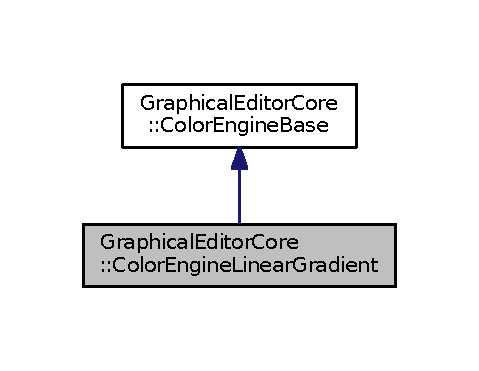
\includegraphics[width=230pt]{classGraphicalEditorCore_1_1ColorEngineLinearGradient__inherit__graph}
\end{center}
\end{figure}


Collaboration diagram for Graphical\+Editor\+Core\+:\+:Color\+Engine\+Linear\+Gradient\+:
\nopagebreak
\begin{figure}[H]
\begin{center}
\leavevmode
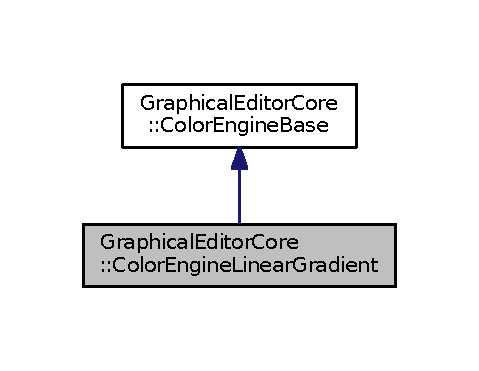
\includegraphics[width=230pt]{classGraphicalEditorCore_1_1ColorEngineLinearGradient__coll__graph}
\end{center}
\end{figure}
\subsection*{Public Member Functions}
\begin{DoxyCompactItemize}
\item 
\hyperlink{classGraphicalEditorCore_1_1ColorEngineLinearGradient_a12f2a422a82b8376d0ddaca148e82e86}{Color\+Engine\+Linear\+Gradient} ()
\item 
virtual \hyperlink{classGraphicalEditorCore_1_1ColorEngineLinearGradient_acb6ceca52590a6c0f06dbe88e8372ee7}{$\sim$\+Color\+Engine\+Linear\+Gradient} ()=default
\item 
virtual uint8\+\_\+t \hyperlink{classGraphicalEditorCore_1_1ColorEngineLinearGradient_acecdc769c65b3ede786edd1a6abe72b5}{red} (const size\+\_\+t i\+\_\+x, const size\+\_\+t j\+\_\+y) const override
\item 
virtual uint8\+\_\+t \hyperlink{classGraphicalEditorCore_1_1ColorEngineLinearGradient_a961e4df71e25e227418a7bcb13c7379b}{green} (const size\+\_\+t i\+\_\+x, const size\+\_\+t j\+\_\+y) const override
\item 
virtual uint8\+\_\+t \hyperlink{classGraphicalEditorCore_1_1ColorEngineLinearGradient_a4a7f4918aa7444b6816c24c42611b157}{blue} (const size\+\_\+t i\+\_\+x, const size\+\_\+t j\+\_\+y) const override
\end{DoxyCompactItemize}


\subsection{Constructor \& Destructor Documentation}
\index{Graphical\+Editor\+Core\+::\+Color\+Engine\+Linear\+Gradient@{Graphical\+Editor\+Core\+::\+Color\+Engine\+Linear\+Gradient}!Color\+Engine\+Linear\+Gradient@{Color\+Engine\+Linear\+Gradient}}
\index{Color\+Engine\+Linear\+Gradient@{Color\+Engine\+Linear\+Gradient}!Graphical\+Editor\+Core\+::\+Color\+Engine\+Linear\+Gradient@{Graphical\+Editor\+Core\+::\+Color\+Engine\+Linear\+Gradient}}
\subsubsection[{\texorpdfstring{Color\+Engine\+Linear\+Gradient()}{ColorEngineLinearGradient()}}]{\setlength{\rightskip}{0pt plus 5cm}Graphical\+Editor\+Core\+::\+Color\+Engine\+Linear\+Gradient\+::\+Color\+Engine\+Linear\+Gradient (
\begin{DoxyParamCaption}
{}
\end{DoxyParamCaption}
)}\hypertarget{classGraphicalEditorCore_1_1ColorEngineLinearGradient_a12f2a422a82b8376d0ddaca148e82e86}{}\label{classGraphicalEditorCore_1_1ColorEngineLinearGradient_a12f2a422a82b8376d0ddaca148e82e86}
\index{Graphical\+Editor\+Core\+::\+Color\+Engine\+Linear\+Gradient@{Graphical\+Editor\+Core\+::\+Color\+Engine\+Linear\+Gradient}!````~Color\+Engine\+Linear\+Gradient@{$\sim$\+Color\+Engine\+Linear\+Gradient}}
\index{````~Color\+Engine\+Linear\+Gradient@{$\sim$\+Color\+Engine\+Linear\+Gradient}!Graphical\+Editor\+Core\+::\+Color\+Engine\+Linear\+Gradient@{Graphical\+Editor\+Core\+::\+Color\+Engine\+Linear\+Gradient}}
\subsubsection[{\texorpdfstring{$\sim$\+Color\+Engine\+Linear\+Gradient()=default}{~ColorEngineLinearGradient()=default}}]{\setlength{\rightskip}{0pt plus 5cm}virtual Graphical\+Editor\+Core\+::\+Color\+Engine\+Linear\+Gradient\+::$\sim$\+Color\+Engine\+Linear\+Gradient (
\begin{DoxyParamCaption}
{}
\end{DoxyParamCaption}
)\hspace{0.3cm}{\ttfamily [virtual]}, {\ttfamily [default]}}\hypertarget{classGraphicalEditorCore_1_1ColorEngineLinearGradient_acb6ceca52590a6c0f06dbe88e8372ee7}{}\label{classGraphicalEditorCore_1_1ColorEngineLinearGradient_acb6ceca52590a6c0f06dbe88e8372ee7}


\subsection{Member Function Documentation}
\index{Graphical\+Editor\+Core\+::\+Color\+Engine\+Linear\+Gradient@{Graphical\+Editor\+Core\+::\+Color\+Engine\+Linear\+Gradient}!blue@{blue}}
\index{blue@{blue}!Graphical\+Editor\+Core\+::\+Color\+Engine\+Linear\+Gradient@{Graphical\+Editor\+Core\+::\+Color\+Engine\+Linear\+Gradient}}
\subsubsection[{\texorpdfstring{blue(const size\+\_\+t i\+\_\+x, const size\+\_\+t j\+\_\+y) const override}{blue(const size_t i_x, const size_t j_y) const override}}]{\setlength{\rightskip}{0pt plus 5cm}uint8\+\_\+t Graphical\+Editor\+Core\+::\+Color\+Engine\+Linear\+Gradient\+::blue (
\begin{DoxyParamCaption}
\item[{const size\+\_\+t}]{i\+\_\+x, }
\item[{const size\+\_\+t}]{j\+\_\+y}
\end{DoxyParamCaption}
) const\hspace{0.3cm}{\ttfamily [override]}, {\ttfamily [virtual]}}\hypertarget{classGraphicalEditorCore_1_1ColorEngineLinearGradient_a4a7f4918aa7444b6816c24c42611b157}{}\label{classGraphicalEditorCore_1_1ColorEngineLinearGradient_a4a7f4918aa7444b6816c24c42611b157}


Implements \hyperlink{classGraphicalEditorCore_1_1ColorEngineBase_a86a1c186366f3df9469e36421167f8cb}{Graphical\+Editor\+Core\+::\+Color\+Engine\+Base}.

\index{Graphical\+Editor\+Core\+::\+Color\+Engine\+Linear\+Gradient@{Graphical\+Editor\+Core\+::\+Color\+Engine\+Linear\+Gradient}!green@{green}}
\index{green@{green}!Graphical\+Editor\+Core\+::\+Color\+Engine\+Linear\+Gradient@{Graphical\+Editor\+Core\+::\+Color\+Engine\+Linear\+Gradient}}
\subsubsection[{\texorpdfstring{green(const size\+\_\+t i\+\_\+x, const size\+\_\+t j\+\_\+y) const override}{green(const size_t i_x, const size_t j_y) const override}}]{\setlength{\rightskip}{0pt plus 5cm}uint8\+\_\+t Graphical\+Editor\+Core\+::\+Color\+Engine\+Linear\+Gradient\+::green (
\begin{DoxyParamCaption}
\item[{const size\+\_\+t}]{i\+\_\+x, }
\item[{const size\+\_\+t}]{j\+\_\+y}
\end{DoxyParamCaption}
) const\hspace{0.3cm}{\ttfamily [override]}, {\ttfamily [virtual]}}\hypertarget{classGraphicalEditorCore_1_1ColorEngineLinearGradient_a961e4df71e25e227418a7bcb13c7379b}{}\label{classGraphicalEditorCore_1_1ColorEngineLinearGradient_a961e4df71e25e227418a7bcb13c7379b}


Implements \hyperlink{classGraphicalEditorCore_1_1ColorEngineBase_a748837e34f2bf4409ae36a5d9ea02e27}{Graphical\+Editor\+Core\+::\+Color\+Engine\+Base}.

\index{Graphical\+Editor\+Core\+::\+Color\+Engine\+Linear\+Gradient@{Graphical\+Editor\+Core\+::\+Color\+Engine\+Linear\+Gradient}!red@{red}}
\index{red@{red}!Graphical\+Editor\+Core\+::\+Color\+Engine\+Linear\+Gradient@{Graphical\+Editor\+Core\+::\+Color\+Engine\+Linear\+Gradient}}
\subsubsection[{\texorpdfstring{red(const size\+\_\+t i\+\_\+x, const size\+\_\+t j\+\_\+y) const override}{red(const size_t i_x, const size_t j_y) const override}}]{\setlength{\rightskip}{0pt plus 5cm}uint8\+\_\+t Graphical\+Editor\+Core\+::\+Color\+Engine\+Linear\+Gradient\+::red (
\begin{DoxyParamCaption}
\item[{const size\+\_\+t}]{i\+\_\+x, }
\item[{const size\+\_\+t}]{j\+\_\+y}
\end{DoxyParamCaption}
) const\hspace{0.3cm}{\ttfamily [override]}, {\ttfamily [virtual]}}\hypertarget{classGraphicalEditorCore_1_1ColorEngineLinearGradient_acecdc769c65b3ede786edd1a6abe72b5}{}\label{classGraphicalEditorCore_1_1ColorEngineLinearGradient_acecdc769c65b3ede786edd1a6abe72b5}


Implements \hyperlink{classGraphicalEditorCore_1_1ColorEngineBase_a9d0b1a48ea117d8f47c43b9c63982dc5}{Graphical\+Editor\+Core\+::\+Color\+Engine\+Base}.



The documentation for this class was generated from the following files\+:\begin{DoxyCompactItemize}
\item 
05\+\_\+editor/\hyperlink{color__engine_8h}{color\+\_\+engine.\+h}\item 
05\+\_\+editor/\hyperlink{color__engine_8cpp}{color\+\_\+engine.\+cpp}\end{DoxyCompactItemize}

\hypertarget{classGraphicalEditorCore_1_1ColorEngineUniform}{}\section{Graphical\+Editor\+Core\+:\+:Color\+Engine\+Uniform Class Reference}
\label{classGraphicalEditorCore_1_1ColorEngineUniform}\index{Graphical\+Editor\+Core\+::\+Color\+Engine\+Uniform@{Graphical\+Editor\+Core\+::\+Color\+Engine\+Uniform}}


{\ttfamily \#include $<$color\+\_\+engine.\+h$>$}



Inheritance diagram for Graphical\+Editor\+Core\+:\+:Color\+Engine\+Uniform\+:
\nopagebreak
\begin{figure}[H]
\begin{center}
\leavevmode
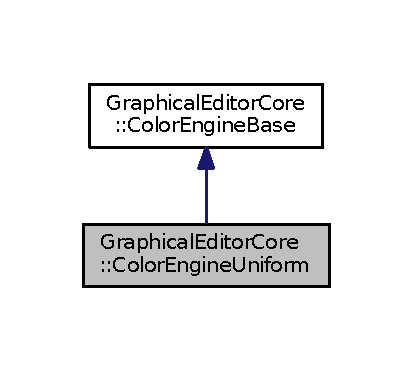
\includegraphics[width=198pt]{classGraphicalEditorCore_1_1ColorEngineUniform__inherit__graph}
\end{center}
\end{figure}


Collaboration diagram for Graphical\+Editor\+Core\+:\+:Color\+Engine\+Uniform\+:
\nopagebreak
\begin{figure}[H]
\begin{center}
\leavevmode
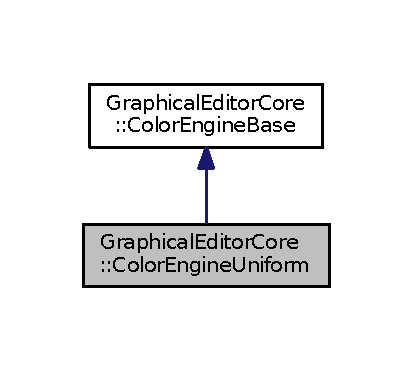
\includegraphics[width=198pt]{classGraphicalEditorCore_1_1ColorEngineUniform__coll__graph}
\end{center}
\end{figure}
\subsection*{Public Member Functions}
\begin{DoxyCompactItemize}
\item 
\hyperlink{classGraphicalEditorCore_1_1ColorEngineUniform_a9e76ad9019e3bb878f6250ca57e2f777}{Color\+Engine\+Uniform} ()
\item 
\hyperlink{classGraphicalEditorCore_1_1ColorEngineUniform_aa91a594076b06d41154b68543870b388}{Color\+Engine\+Uniform} (const uint8\+\_\+t r, const uint8\+\_\+t g, const uint8\+\_\+t b)
\item 
virtual \hyperlink{classGraphicalEditorCore_1_1ColorEngineUniform_a0bfdba9e4751b79bdcf9692ad57fde34}{$\sim$\+Color\+Engine\+Uniform} ()=default
\item 
virtual uint8\+\_\+t \hyperlink{classGraphicalEditorCore_1_1ColorEngineUniform_a91461ce9955811e4e5e2f74cd2e9ec94}{red} (const size\+\_\+t i\+\_\+x, const size\+\_\+t j\+\_\+y) const override
\item 
virtual uint8\+\_\+t \hyperlink{classGraphicalEditorCore_1_1ColorEngineUniform_a219f34e3e5dabdf260e7c1adaa8bc2ee}{green} (const size\+\_\+t i\+\_\+x, const size\+\_\+t j\+\_\+y) const override
\item 
virtual uint8\+\_\+t \hyperlink{classGraphicalEditorCore_1_1ColorEngineUniform_ae5d9b3422740f667080f28d22a17830b}{blue} (const size\+\_\+t i\+\_\+x, const size\+\_\+t j\+\_\+y) const override
\end{DoxyCompactItemize}


\subsection{Constructor \& Destructor Documentation}
\index{Graphical\+Editor\+Core\+::\+Color\+Engine\+Uniform@{Graphical\+Editor\+Core\+::\+Color\+Engine\+Uniform}!Color\+Engine\+Uniform@{Color\+Engine\+Uniform}}
\index{Color\+Engine\+Uniform@{Color\+Engine\+Uniform}!Graphical\+Editor\+Core\+::\+Color\+Engine\+Uniform@{Graphical\+Editor\+Core\+::\+Color\+Engine\+Uniform}}
\subsubsection[{\texorpdfstring{Color\+Engine\+Uniform()}{ColorEngineUniform()}}]{\setlength{\rightskip}{0pt plus 5cm}Graphical\+Editor\+Core\+::\+Color\+Engine\+Uniform\+::\+Color\+Engine\+Uniform (
\begin{DoxyParamCaption}
{}
\end{DoxyParamCaption}
)}\hypertarget{classGraphicalEditorCore_1_1ColorEngineUniform_a9e76ad9019e3bb878f6250ca57e2f777}{}\label{classGraphicalEditorCore_1_1ColorEngineUniform_a9e76ad9019e3bb878f6250ca57e2f777}
\index{Graphical\+Editor\+Core\+::\+Color\+Engine\+Uniform@{Graphical\+Editor\+Core\+::\+Color\+Engine\+Uniform}!Color\+Engine\+Uniform@{Color\+Engine\+Uniform}}
\index{Color\+Engine\+Uniform@{Color\+Engine\+Uniform}!Graphical\+Editor\+Core\+::\+Color\+Engine\+Uniform@{Graphical\+Editor\+Core\+::\+Color\+Engine\+Uniform}}
\subsubsection[{\texorpdfstring{Color\+Engine\+Uniform(const uint8\+\_\+t r, const uint8\+\_\+t g, const uint8\+\_\+t b)}{ColorEngineUniform(const uint8_t r, const uint8_t g, const uint8_t b)}}]{\setlength{\rightskip}{0pt plus 5cm}Graphical\+Editor\+Core\+::\+Color\+Engine\+Uniform\+::\+Color\+Engine\+Uniform (
\begin{DoxyParamCaption}
\item[{const uint8\+\_\+t}]{r, }
\item[{const uint8\+\_\+t}]{g, }
\item[{const uint8\+\_\+t}]{b}
\end{DoxyParamCaption}
)}\hypertarget{classGraphicalEditorCore_1_1ColorEngineUniform_aa91a594076b06d41154b68543870b388}{}\label{classGraphicalEditorCore_1_1ColorEngineUniform_aa91a594076b06d41154b68543870b388}
\index{Graphical\+Editor\+Core\+::\+Color\+Engine\+Uniform@{Graphical\+Editor\+Core\+::\+Color\+Engine\+Uniform}!````~Color\+Engine\+Uniform@{$\sim$\+Color\+Engine\+Uniform}}
\index{````~Color\+Engine\+Uniform@{$\sim$\+Color\+Engine\+Uniform}!Graphical\+Editor\+Core\+::\+Color\+Engine\+Uniform@{Graphical\+Editor\+Core\+::\+Color\+Engine\+Uniform}}
\subsubsection[{\texorpdfstring{$\sim$\+Color\+Engine\+Uniform()=default}{~ColorEngineUniform()=default}}]{\setlength{\rightskip}{0pt plus 5cm}virtual Graphical\+Editor\+Core\+::\+Color\+Engine\+Uniform\+::$\sim$\+Color\+Engine\+Uniform (
\begin{DoxyParamCaption}
{}
\end{DoxyParamCaption}
)\hspace{0.3cm}{\ttfamily [virtual]}, {\ttfamily [default]}}\hypertarget{classGraphicalEditorCore_1_1ColorEngineUniform_a0bfdba9e4751b79bdcf9692ad57fde34}{}\label{classGraphicalEditorCore_1_1ColorEngineUniform_a0bfdba9e4751b79bdcf9692ad57fde34}


\subsection{Member Function Documentation}
\index{Graphical\+Editor\+Core\+::\+Color\+Engine\+Uniform@{Graphical\+Editor\+Core\+::\+Color\+Engine\+Uniform}!blue@{blue}}
\index{blue@{blue}!Graphical\+Editor\+Core\+::\+Color\+Engine\+Uniform@{Graphical\+Editor\+Core\+::\+Color\+Engine\+Uniform}}
\subsubsection[{\texorpdfstring{blue(const size\+\_\+t i\+\_\+x, const size\+\_\+t j\+\_\+y) const override}{blue(const size_t i_x, const size_t j_y) const override}}]{\setlength{\rightskip}{0pt plus 5cm}uint8\+\_\+t Graphical\+Editor\+Core\+::\+Color\+Engine\+Uniform\+::blue (
\begin{DoxyParamCaption}
\item[{const size\+\_\+t}]{i\+\_\+x, }
\item[{const size\+\_\+t}]{j\+\_\+y}
\end{DoxyParamCaption}
) const\hspace{0.3cm}{\ttfamily [override]}, {\ttfamily [virtual]}}\hypertarget{classGraphicalEditorCore_1_1ColorEngineUniform_ae5d9b3422740f667080f28d22a17830b}{}\label{classGraphicalEditorCore_1_1ColorEngineUniform_ae5d9b3422740f667080f28d22a17830b}


Implements \hyperlink{classGraphicalEditorCore_1_1ColorEngineBase_a86a1c186366f3df9469e36421167f8cb}{Graphical\+Editor\+Core\+::\+Color\+Engine\+Base}.

\index{Graphical\+Editor\+Core\+::\+Color\+Engine\+Uniform@{Graphical\+Editor\+Core\+::\+Color\+Engine\+Uniform}!green@{green}}
\index{green@{green}!Graphical\+Editor\+Core\+::\+Color\+Engine\+Uniform@{Graphical\+Editor\+Core\+::\+Color\+Engine\+Uniform}}
\subsubsection[{\texorpdfstring{green(const size\+\_\+t i\+\_\+x, const size\+\_\+t j\+\_\+y) const override}{green(const size_t i_x, const size_t j_y) const override}}]{\setlength{\rightskip}{0pt plus 5cm}uint8\+\_\+t Graphical\+Editor\+Core\+::\+Color\+Engine\+Uniform\+::green (
\begin{DoxyParamCaption}
\item[{const size\+\_\+t}]{i\+\_\+x, }
\item[{const size\+\_\+t}]{j\+\_\+y}
\end{DoxyParamCaption}
) const\hspace{0.3cm}{\ttfamily [override]}, {\ttfamily [virtual]}}\hypertarget{classGraphicalEditorCore_1_1ColorEngineUniform_a219f34e3e5dabdf260e7c1adaa8bc2ee}{}\label{classGraphicalEditorCore_1_1ColorEngineUniform_a219f34e3e5dabdf260e7c1adaa8bc2ee}


Implements \hyperlink{classGraphicalEditorCore_1_1ColorEngineBase_a748837e34f2bf4409ae36a5d9ea02e27}{Graphical\+Editor\+Core\+::\+Color\+Engine\+Base}.

\index{Graphical\+Editor\+Core\+::\+Color\+Engine\+Uniform@{Graphical\+Editor\+Core\+::\+Color\+Engine\+Uniform}!red@{red}}
\index{red@{red}!Graphical\+Editor\+Core\+::\+Color\+Engine\+Uniform@{Graphical\+Editor\+Core\+::\+Color\+Engine\+Uniform}}
\subsubsection[{\texorpdfstring{red(const size\+\_\+t i\+\_\+x, const size\+\_\+t j\+\_\+y) const override}{red(const size_t i_x, const size_t j_y) const override}}]{\setlength{\rightskip}{0pt plus 5cm}uint8\+\_\+t Graphical\+Editor\+Core\+::\+Color\+Engine\+Uniform\+::red (
\begin{DoxyParamCaption}
\item[{const size\+\_\+t}]{i\+\_\+x, }
\item[{const size\+\_\+t}]{j\+\_\+y}
\end{DoxyParamCaption}
) const\hspace{0.3cm}{\ttfamily [override]}, {\ttfamily [virtual]}}\hypertarget{classGraphicalEditorCore_1_1ColorEngineUniform_a91461ce9955811e4e5e2f74cd2e9ec94}{}\label{classGraphicalEditorCore_1_1ColorEngineUniform_a91461ce9955811e4e5e2f74cd2e9ec94}


Implements \hyperlink{classGraphicalEditorCore_1_1ColorEngineBase_a9d0b1a48ea117d8f47c43b9c63982dc5}{Graphical\+Editor\+Core\+::\+Color\+Engine\+Base}.



The documentation for this class was generated from the following files\+:\begin{DoxyCompactItemize}
\item 
05\+\_\+editor/\hyperlink{color__engine_8h}{color\+\_\+engine.\+h}\item 
05\+\_\+editor/\hyperlink{color__engine_8cpp}{color\+\_\+engine.\+cpp}\end{DoxyCompactItemize}

\hypertarget{classGraphicalEditorCore_1_1CompositeShape2D}{}\section{Graphical\+Editor\+Core\+:\+:Composite\+Shape2D$<$ T $>$ Class Template Reference}
\label{classGraphicalEditorCore_1_1CompositeShape2D}\index{Graphical\+Editor\+Core\+::\+Composite\+Shape2\+D$<$ T $>$@{Graphical\+Editor\+Core\+::\+Composite\+Shape2\+D$<$ T $>$}}


{\ttfamily \#include $<$shapes\+\_\+2d.\+h$>$}



Inheritance diagram for Graphical\+Editor\+Core\+:\+:Composite\+Shape2D$<$ T $>$\+:
\nopagebreak
\begin{figure}[H]
\begin{center}
\leavevmode
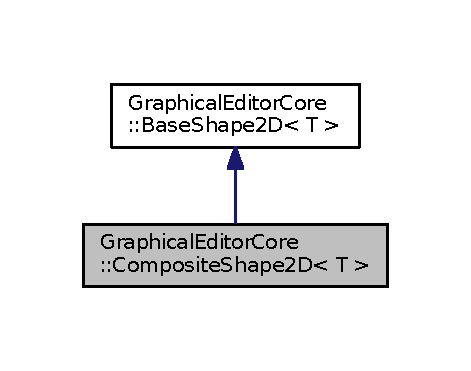
\includegraphics[width=226pt]{classGraphicalEditorCore_1_1CompositeShape2D__inherit__graph}
\end{center}
\end{figure}


Collaboration diagram for Graphical\+Editor\+Core\+:\+:Composite\+Shape2D$<$ T $>$\+:
\nopagebreak
\begin{figure}[H]
\begin{center}
\leavevmode
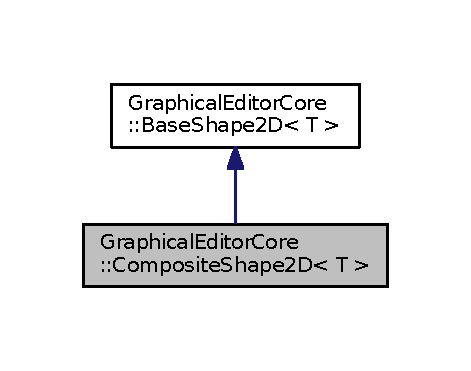
\includegraphics[width=226pt]{classGraphicalEditorCore_1_1CompositeShape2D__coll__graph}
\end{center}
\end{figure}
\subsection*{Public Member Functions}
\begin{DoxyCompactItemize}
\item 
\hyperlink{classGraphicalEditorCore_1_1CompositeShape2D_af8dcc9f1047e1594cfbe61b62dd6a0ce}{Composite\+Shape2D} (const size\+\_\+t \hyperlink{classGraphicalEditorCore_1_1BaseShape2D_ac66cfa23289ae36d70ff6b7c41dd791f}{id})
\item 
virtual \hyperlink{classGraphicalEditorCore_1_1CompositeShape2D_a0a5658b8caf83f1578ed32b762e5db2c}{$\sim$\+Composite\+Shape2D} ()
\item 
void \hyperlink{classGraphicalEditorCore_1_1CompositeShape2D_afa65e170aed5aa31d67b1f541c24f656}{add} (std\+::unique\+\_\+ptr$<$ \hyperlink{classGraphicalEditorCore_1_1BaseShape2D}{Base\+Shape2D}$<$ T $>$$>$ \&\&shape\+\_\+composite\+\_\+2d)
\item 
\hyperlink{classGraphicalEditorCore_1_1BaseShape2D}{Base\+Shape2D}$<$ T $>$ \& \hyperlink{classGraphicalEditorCore_1_1CompositeShape2D_a4cfefba661a2a6652ec2554e77ecba71}{shape2d} (const size\+\_\+t \hyperlink{classGraphicalEditorCore_1_1BaseShape2D_ac66cfa23289ae36d70ff6b7c41dd791f}{id})
\item 
virtual void \hyperlink{classGraphicalEditorCore_1_1CompositeShape2D_a1ad124ab5448a4276d06742318744473}{rotate} (const T clockwise\+\_\+angle) override
\item 
virtual void \hyperlink{classGraphicalEditorCore_1_1CompositeShape2D_a16cb9751cbd8f587f7f68ce831314e14}{move\+Center} (const T dx, const T dy) override
\item 
virtual void \hyperlink{classGraphicalEditorCore_1_1CompositeShape2D_a2754d592f39a2c442681fad8039e682f}{move\+Vertex} (const T dx, const T dy, const size\+\_\+t index) override
\item 
virtual void \hyperlink{classGraphicalEditorCore_1_1CompositeShape2D_ae1d0a3270ae8eeec8a87c5a37d657336}{scale} (const T factor) override
\item 
virtual void \hyperlink{classGraphicalEditorCore_1_1CompositeShape2D_af0ed12595f25239559d340c81d0fcb0d}{append} (\hyperlink{classGraphicalEditorCore_1_1DocumentWriterBase}{Document\+Writer\+Base} \&) const override
\end{DoxyCompactItemize}


\subsection{Constructor \& Destructor Documentation}
\index{Graphical\+Editor\+Core\+::\+Composite\+Shape2D@{Graphical\+Editor\+Core\+::\+Composite\+Shape2D}!Composite\+Shape2D@{Composite\+Shape2D}}
\index{Composite\+Shape2D@{Composite\+Shape2D}!Graphical\+Editor\+Core\+::\+Composite\+Shape2D@{Graphical\+Editor\+Core\+::\+Composite\+Shape2D}}
\subsubsection[{\texorpdfstring{Composite\+Shape2\+D(const size\+\_\+t id)}{CompositeShape2D(const size_t id)}}]{\setlength{\rightskip}{0pt plus 5cm}template$<$typename T $>$ {\bf Graphical\+Editor\+Core\+::\+Composite\+Shape2D}$<$ T $>$\+::{\bf Composite\+Shape2D} (
\begin{DoxyParamCaption}
\item[{const size\+\_\+t}]{id}
\end{DoxyParamCaption}
)}\hypertarget{classGraphicalEditorCore_1_1CompositeShape2D_af8dcc9f1047e1594cfbe61b62dd6a0ce}{}\label{classGraphicalEditorCore_1_1CompositeShape2D_af8dcc9f1047e1594cfbe61b62dd6a0ce}
\index{Graphical\+Editor\+Core\+::\+Composite\+Shape2D@{Graphical\+Editor\+Core\+::\+Composite\+Shape2D}!````~Composite\+Shape2D@{$\sim$\+Composite\+Shape2D}}
\index{````~Composite\+Shape2D@{$\sim$\+Composite\+Shape2D}!Graphical\+Editor\+Core\+::\+Composite\+Shape2D@{Graphical\+Editor\+Core\+::\+Composite\+Shape2D}}
\subsubsection[{\texorpdfstring{$\sim$\+Composite\+Shape2\+D()}{~CompositeShape2D()}}]{\setlength{\rightskip}{0pt plus 5cm}template$<$typename T $>$ {\bf Graphical\+Editor\+Core\+::\+Composite\+Shape2D}$<$ T $>$\+::$\sim${\bf Composite\+Shape2D} (
\begin{DoxyParamCaption}
{}
\end{DoxyParamCaption}
)\hspace{0.3cm}{\ttfamily [virtual]}}\hypertarget{classGraphicalEditorCore_1_1CompositeShape2D_a0a5658b8caf83f1578ed32b762e5db2c}{}\label{classGraphicalEditorCore_1_1CompositeShape2D_a0a5658b8caf83f1578ed32b762e5db2c}


\subsection{Member Function Documentation}
\index{Graphical\+Editor\+Core\+::\+Composite\+Shape2D@{Graphical\+Editor\+Core\+::\+Composite\+Shape2D}!add@{add}}
\index{add@{add}!Graphical\+Editor\+Core\+::\+Composite\+Shape2D@{Graphical\+Editor\+Core\+::\+Composite\+Shape2D}}
\subsubsection[{\texorpdfstring{add(std\+::unique\+\_\+ptr$<$ Base\+Shape2\+D$<$ T $>$$>$ \&\&shape\+\_\+composite\+\_\+2d)}{add(std::unique_ptr< BaseShape2D< T >> &&shape_composite_2d)}}]{\setlength{\rightskip}{0pt plus 5cm}template$<$typename T $>$ void {\bf Graphical\+Editor\+Core\+::\+Composite\+Shape2D}$<$ T $>$\+::add (
\begin{DoxyParamCaption}
\item[{std\+::unique\+\_\+ptr$<$ {\bf Base\+Shape2D}$<$ T $>$$>$ \&\&}]{shape\+\_\+composite\+\_\+2d}
\end{DoxyParamCaption}
)}\hypertarget{classGraphicalEditorCore_1_1CompositeShape2D_afa65e170aed5aa31d67b1f541c24f656}{}\label{classGraphicalEditorCore_1_1CompositeShape2D_afa65e170aed5aa31d67b1f541c24f656}
\index{Graphical\+Editor\+Core\+::\+Composite\+Shape2D@{Graphical\+Editor\+Core\+::\+Composite\+Shape2D}!append@{append}}
\index{append@{append}!Graphical\+Editor\+Core\+::\+Composite\+Shape2D@{Graphical\+Editor\+Core\+::\+Composite\+Shape2D}}
\subsubsection[{\texorpdfstring{append(\+Document\+Writer\+Base \&) const override}{append(DocumentWriterBase &) const override}}]{\setlength{\rightskip}{0pt plus 5cm}template$<$typename T $>$ void {\bf Graphical\+Editor\+Core\+::\+Composite\+Shape2D}$<$ T $>$\+::append (
\begin{DoxyParamCaption}
\item[{{\bf Document\+Writer\+Base} \&}]{wr\+\_\+eng}
\end{DoxyParamCaption}
) const\hspace{0.3cm}{\ttfamily [override]}, {\ttfamily [virtual]}}\hypertarget{classGraphicalEditorCore_1_1CompositeShape2D_af0ed12595f25239559d340c81d0fcb0d}{}\label{classGraphicalEditorCore_1_1CompositeShape2D_af0ed12595f25239559d340c81d0fcb0d}


Reimplemented from \hyperlink{classGraphicalEditorCore_1_1BaseShape2D_ac8f67c255fe72fd97aa7a5df80b698be}{Graphical\+Editor\+Core\+::\+Base\+Shape2\+D$<$ T $>$}.

\index{Graphical\+Editor\+Core\+::\+Composite\+Shape2D@{Graphical\+Editor\+Core\+::\+Composite\+Shape2D}!move\+Center@{move\+Center}}
\index{move\+Center@{move\+Center}!Graphical\+Editor\+Core\+::\+Composite\+Shape2D@{Graphical\+Editor\+Core\+::\+Composite\+Shape2D}}
\subsubsection[{\texorpdfstring{move\+Center(const T dx, const T dy) override}{moveCenter(const T dx, const T dy) override}}]{\setlength{\rightskip}{0pt plus 5cm}template$<$typename T $>$ void {\bf Graphical\+Editor\+Core\+::\+Composite\+Shape2D}$<$ T $>$\+::move\+Center (
\begin{DoxyParamCaption}
\item[{const T}]{dx, }
\item[{const T}]{dy}
\end{DoxyParamCaption}
)\hspace{0.3cm}{\ttfamily [override]}, {\ttfamily [virtual]}}\hypertarget{classGraphicalEditorCore_1_1CompositeShape2D_a16cb9751cbd8f587f7f68ce831314e14}{}\label{classGraphicalEditorCore_1_1CompositeShape2D_a16cb9751cbd8f587f7f68ce831314e14}


Implements \hyperlink{classGraphicalEditorCore_1_1BaseShape2D_adebef5c637da2c34a2fe728022740f94}{Graphical\+Editor\+Core\+::\+Base\+Shape2\+D$<$ T $>$}.

\index{Graphical\+Editor\+Core\+::\+Composite\+Shape2D@{Graphical\+Editor\+Core\+::\+Composite\+Shape2D}!move\+Vertex@{move\+Vertex}}
\index{move\+Vertex@{move\+Vertex}!Graphical\+Editor\+Core\+::\+Composite\+Shape2D@{Graphical\+Editor\+Core\+::\+Composite\+Shape2D}}
\subsubsection[{\texorpdfstring{move\+Vertex(const T dx, const T dy, const size\+\_\+t index) override}{moveVertex(const T dx, const T dy, const size_t index) override}}]{\setlength{\rightskip}{0pt plus 5cm}template$<$typename T $>$ void {\bf Graphical\+Editor\+Core\+::\+Composite\+Shape2D}$<$ T $>$\+::move\+Vertex (
\begin{DoxyParamCaption}
\item[{const T}]{dx, }
\item[{const T}]{dy, }
\item[{const size\+\_\+t}]{index}
\end{DoxyParamCaption}
)\hspace{0.3cm}{\ttfamily [override]}, {\ttfamily [virtual]}}\hypertarget{classGraphicalEditorCore_1_1CompositeShape2D_a2754d592f39a2c442681fad8039e682f}{}\label{classGraphicalEditorCore_1_1CompositeShape2D_a2754d592f39a2c442681fad8039e682f}


Implements \hyperlink{classGraphicalEditorCore_1_1BaseShape2D_a9e6394ecf62e475a1d087e89258d4131}{Graphical\+Editor\+Core\+::\+Base\+Shape2\+D$<$ T $>$}.

\index{Graphical\+Editor\+Core\+::\+Composite\+Shape2D@{Graphical\+Editor\+Core\+::\+Composite\+Shape2D}!rotate@{rotate}}
\index{rotate@{rotate}!Graphical\+Editor\+Core\+::\+Composite\+Shape2D@{Graphical\+Editor\+Core\+::\+Composite\+Shape2D}}
\subsubsection[{\texorpdfstring{rotate(const T clockwise\+\_\+angle) override}{rotate(const T clockwise_angle) override}}]{\setlength{\rightskip}{0pt plus 5cm}template$<$typename T $>$ void {\bf Graphical\+Editor\+Core\+::\+Composite\+Shape2D}$<$ T $>$\+::rotate (
\begin{DoxyParamCaption}
\item[{const T}]{clockwise\+\_\+angle}
\end{DoxyParamCaption}
)\hspace{0.3cm}{\ttfamily [override]}, {\ttfamily [virtual]}}\hypertarget{classGraphicalEditorCore_1_1CompositeShape2D_a1ad124ab5448a4276d06742318744473}{}\label{classGraphicalEditorCore_1_1CompositeShape2D_a1ad124ab5448a4276d06742318744473}


Implements \hyperlink{classGraphicalEditorCore_1_1BaseShape2D_a94a87b2fd8485cfb7d4ca97050d1bdde}{Graphical\+Editor\+Core\+::\+Base\+Shape2\+D$<$ T $>$}.

\index{Graphical\+Editor\+Core\+::\+Composite\+Shape2D@{Graphical\+Editor\+Core\+::\+Composite\+Shape2D}!scale@{scale}}
\index{scale@{scale}!Graphical\+Editor\+Core\+::\+Composite\+Shape2D@{Graphical\+Editor\+Core\+::\+Composite\+Shape2D}}
\subsubsection[{\texorpdfstring{scale(const T factor) override}{scale(const T factor) override}}]{\setlength{\rightskip}{0pt plus 5cm}template$<$typename T $>$ void {\bf Graphical\+Editor\+Core\+::\+Composite\+Shape2D}$<$ T $>$\+::scale (
\begin{DoxyParamCaption}
\item[{const T}]{factor}
\end{DoxyParamCaption}
)\hspace{0.3cm}{\ttfamily [override]}, {\ttfamily [virtual]}}\hypertarget{classGraphicalEditorCore_1_1CompositeShape2D_ae1d0a3270ae8eeec8a87c5a37d657336}{}\label{classGraphicalEditorCore_1_1CompositeShape2D_ae1d0a3270ae8eeec8a87c5a37d657336}


Implements \hyperlink{classGraphicalEditorCore_1_1BaseShape2D_a2ff960ec57b180222a084642fa7dc780}{Graphical\+Editor\+Core\+::\+Base\+Shape2\+D$<$ T $>$}.

\index{Graphical\+Editor\+Core\+::\+Composite\+Shape2D@{Graphical\+Editor\+Core\+::\+Composite\+Shape2D}!shape2d@{shape2d}}
\index{shape2d@{shape2d}!Graphical\+Editor\+Core\+::\+Composite\+Shape2D@{Graphical\+Editor\+Core\+::\+Composite\+Shape2D}}
\subsubsection[{\texorpdfstring{shape2d(const size\+\_\+t id)}{shape2d(const size_t id)}}]{\setlength{\rightskip}{0pt plus 5cm}template$<$typename T $>$ {\bf Base\+Shape2D}$<$ T $>$ \& {\bf Graphical\+Editor\+Core\+::\+Composite\+Shape2D}$<$ T $>$\+::shape2d (
\begin{DoxyParamCaption}
\item[{const size\+\_\+t}]{id}
\end{DoxyParamCaption}
)}\hypertarget{classGraphicalEditorCore_1_1CompositeShape2D_a4cfefba661a2a6652ec2554e77ecba71}{}\label{classGraphicalEditorCore_1_1CompositeShape2D_a4cfefba661a2a6652ec2554e77ecba71}


The documentation for this class was generated from the following files\+:\begin{DoxyCompactItemize}
\item 
05\+\_\+editor/\hyperlink{shapes__2d_8h}{shapes\+\_\+2d.\+h}\item 
05\+\_\+editor/\hyperlink{composite__shape__2d_8cpp}{composite\+\_\+shape\+\_\+2d.\+cpp}\end{DoxyCompactItemize}

\hypertarget{classcontigious__block}{}\section{contigious\+\_\+block$<$ T $>$ Class Template Reference}
\label{classcontigious__block}\index{contigious\+\_\+block$<$ T $>$@{contigious\+\_\+block$<$ T $>$}}


{\ttfamily \#include $<$flexible\+\_\+allocator.\+hpp$>$}

\subsection*{Public Member Functions}
\begin{DoxyCompactItemize}
\item 
\hyperlink{classcontigious__block_a6357ef263d76c0fcbec77c152365bf59}{contigious\+\_\+block} (const size\+\_\+t)
\item 
\hyperlink{classcontigious__block_abf42cd806e0612249e48f27bedbb3414}{contigious\+\_\+block} (\hyperlink{classcontigious__block}{contigious\+\_\+block} \&\&)
\item 
\hyperlink{classcontigious__block_a5fe8250399873d760c8bbf0b08e51189}{$\sim$contigious\+\_\+block} ()
\item 
const size\+\_\+t \hyperlink{classcontigious__block_a8f083228ca1fbebd733aa93252d258cb}{size} () const 
\item 
T $\ast$ \hyperlink{classcontigious__block_a06e64e88c86a46d3318d2ca5c8ce7461}{base\+\_\+address} ()
\item 
const T $\ast$ \hyperlink{classcontigious__block_ad9de6718dd6824657d9766c9395eaeb2}{base\+\_\+address} () const 
\end{DoxyCompactItemize}


\subsection{Constructor \& Destructor Documentation}
\index{contigious\+\_\+block@{contigious\+\_\+block}!contigious\+\_\+block@{contigious\+\_\+block}}
\index{contigious\+\_\+block@{contigious\+\_\+block}!contigious\+\_\+block@{contigious\+\_\+block}}
\subsubsection[{\texorpdfstring{contigious\+\_\+block(const size\+\_\+t)}{contigious_block(const size_t)}}]{\setlength{\rightskip}{0pt plus 5cm}template$<$typename T $>$ {\bf contigious\+\_\+block}$<$ T $>$\+::{\bf contigious\+\_\+block} (
\begin{DoxyParamCaption}
\item[{const size\+\_\+t}]{size}
\end{DoxyParamCaption}
)}\hypertarget{classcontigious__block_a6357ef263d76c0fcbec77c152365bf59}{}\label{classcontigious__block_a6357ef263d76c0fcbec77c152365bf59}
\index{contigious\+\_\+block@{contigious\+\_\+block}!contigious\+\_\+block@{contigious\+\_\+block}}
\index{contigious\+\_\+block@{contigious\+\_\+block}!contigious\+\_\+block@{contigious\+\_\+block}}
\subsubsection[{\texorpdfstring{contigious\+\_\+block(contigious\+\_\+block \&\&)}{contigious_block(contigious_block &&)}}]{\setlength{\rightskip}{0pt plus 5cm}template$<$typename T $>$ {\bf contigious\+\_\+block}$<$ T $>$\+::{\bf contigious\+\_\+block} (
\begin{DoxyParamCaption}
\item[{{\bf contigious\+\_\+block}$<$ T $>$ \&\&}]{rhs}
\end{DoxyParamCaption}
)}\hypertarget{classcontigious__block_abf42cd806e0612249e48f27bedbb3414}{}\label{classcontigious__block_abf42cd806e0612249e48f27bedbb3414}
\index{contigious\+\_\+block@{contigious\+\_\+block}!````~contigious\+\_\+block@{$\sim$contigious\+\_\+block}}
\index{````~contigious\+\_\+block@{$\sim$contigious\+\_\+block}!contigious\+\_\+block@{contigious\+\_\+block}}
\subsubsection[{\texorpdfstring{$\sim$contigious\+\_\+block()}{~contigious_block()}}]{\setlength{\rightskip}{0pt plus 5cm}template$<$typename T $>$ {\bf contigious\+\_\+block}$<$ T $>$\+::$\sim${\bf contigious\+\_\+block} (
\begin{DoxyParamCaption}
{}
\end{DoxyParamCaption}
)}\hypertarget{classcontigious__block_a5fe8250399873d760c8bbf0b08e51189}{}\label{classcontigious__block_a5fe8250399873d760c8bbf0b08e51189}


\subsection{Member Function Documentation}
\index{contigious\+\_\+block@{contigious\+\_\+block}!base\+\_\+address@{base\+\_\+address}}
\index{base\+\_\+address@{base\+\_\+address}!contigious\+\_\+block@{contigious\+\_\+block}}
\subsubsection[{\texorpdfstring{base\+\_\+address()}{base_address()}}]{\setlength{\rightskip}{0pt plus 5cm}template$<$typename T $>$ T $\ast$ {\bf contigious\+\_\+block}$<$ T $>$\+::base\+\_\+address (
\begin{DoxyParamCaption}
{}
\end{DoxyParamCaption}
)}\hypertarget{classcontigious__block_a06e64e88c86a46d3318d2ca5c8ce7461}{}\label{classcontigious__block_a06e64e88c86a46d3318d2ca5c8ce7461}
\index{contigious\+\_\+block@{contigious\+\_\+block}!base\+\_\+address@{base\+\_\+address}}
\index{base\+\_\+address@{base\+\_\+address}!contigious\+\_\+block@{contigious\+\_\+block}}
\subsubsection[{\texorpdfstring{base\+\_\+address() const }{base_address() const }}]{\setlength{\rightskip}{0pt plus 5cm}template$<$typename T $>$ const T $\ast$ {\bf contigious\+\_\+block}$<$ T $>$\+::base\+\_\+address (
\begin{DoxyParamCaption}
{}
\end{DoxyParamCaption}
) const}\hypertarget{classcontigious__block_ad9de6718dd6824657d9766c9395eaeb2}{}\label{classcontigious__block_ad9de6718dd6824657d9766c9395eaeb2}
\index{contigious\+\_\+block@{contigious\+\_\+block}!size@{size}}
\index{size@{size}!contigious\+\_\+block@{contigious\+\_\+block}}
\subsubsection[{\texorpdfstring{size() const }{size() const }}]{\setlength{\rightskip}{0pt plus 5cm}template$<$typename T $>$ const size\+\_\+t {\bf contigious\+\_\+block}$<$ T $>$\+::size (
\begin{DoxyParamCaption}
{}
\end{DoxyParamCaption}
) const}\hypertarget{classcontigious__block_a8f083228ca1fbebd733aa93252d258cb}{}\label{classcontigious__block_a8f083228ca1fbebd733aa93252d258cb}


The documentation for this class was generated from the following file\+:\begin{DoxyCompactItemize}
\item 
03\+\_\+allocator/\hyperlink{flexible__allocator_8hpp}{flexible\+\_\+allocator.\+hpp}\end{DoxyCompactItemize}

\hypertarget{structcustom__tuple}{}\section{custom\+\_\+tuple$<$ Types $>$ Struct Template Reference}
\label{structcustom__tuple}\index{custom\+\_\+tuple$<$ Types $>$@{custom\+\_\+tuple$<$ Types $>$}}


{\ttfamily \#include $<$cstm\+\_\+tuple.\+hpp$>$}



The documentation for this struct was generated from the following file\+:\begin{DoxyCompactItemize}
\item 
02\+\_\+tuple/\hyperlink{cstm__tuple_8hpp}{cstm\+\_\+tuple.\+hpp}\end{DoxyCompactItemize}

\hypertarget{structcustom__tuple_3_01T_00_01Types_8_8_8_01_4}{}\section{custom\+\_\+tuple$<$ T, Types... $>$ Struct Template Reference}
\label{structcustom__tuple_3_01T_00_01Types_8_8_8_01_4}\index{custom\+\_\+tuple$<$ T, Types... $>$@{custom\+\_\+tuple$<$ T, Types... $>$}}


{\ttfamily \#include $<$cstm\+\_\+tuple.\+hpp$>$}



Inheritance diagram for custom\+\_\+tuple$<$ T, Types... $>$\+:
\nopagebreak
\begin{figure}[H]
\begin{center}
\leavevmode
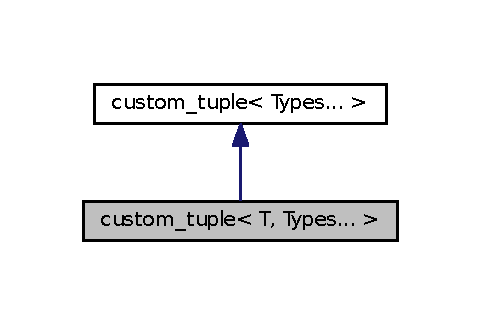
\includegraphics[width=231pt]{structcustom__tuple_3_01T_00_01Types_8_8_8_01_4__inherit__graph}
\end{center}
\end{figure}


Collaboration diagram for custom\+\_\+tuple$<$ T, Types... $>$\+:
\nopagebreak
\begin{figure}[H]
\begin{center}
\leavevmode
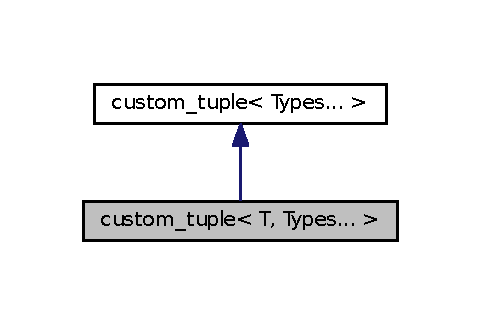
\includegraphics[width=231pt]{structcustom__tuple_3_01T_00_01Types_8_8_8_01_4__coll__graph}
\end{center}
\end{figure}
\subsection*{Public Member Functions}
\begin{DoxyCompactItemize}
\item 
\hyperlink{structcustom__tuple_3_01T_00_01Types_8_8_8_01_4_a89f0b4cc59a4efeb82f0160541708f9a}{custom\+\_\+tuple} (T t\+\_\+arg, Types...\+ts\+\_\+args)
\item 
{\footnotesize template$<$typename Arg1 , typename... Args$>$ }\\\hyperlink{structcustom__tuple}{custom\+\_\+tuple} \& \hyperlink{structcustom__tuple_3_01T_00_01Types_8_8_8_01_4_a40eac7f8ba44f72911adfad9239f91df}{operator=} (const \hyperlink{structcustom__tuple}{custom\+\_\+tuple}$<$ Arg1, Args... $>$ \&rhs)
\item 
{\footnotesize template$<$typename Arg1 , typename... Args$>$ }\\\hyperlink{structcustom__tuple}{custom\+\_\+tuple}$<$ T, Types... $>$ \& \hyperlink{structcustom__tuple_3_01T_00_01Types_8_8_8_01_4_a5bc95f94e20d4b02e3c80eef3e2f7036}{operator=} (const \hyperlink{structcustom__tuple}{custom\+\_\+tuple}$<$ Arg1, Args... $>$ \&rhs)
\end{DoxyCompactItemize}
\subsection*{Public Attributes}
\begin{DoxyCompactItemize}
\item 
T \hyperlink{structcustom__tuple_3_01T_00_01Types_8_8_8_01_4_adff61bc9ff136d4c8393278eef6b62b4}{tail}
\end{DoxyCompactItemize}


\subsection{Constructor \& Destructor Documentation}
\index{custom\+\_\+tuple$<$ T, Types... $>$@{custom\+\_\+tuple$<$ T, Types... $>$}!custom\+\_\+tuple@{custom\+\_\+tuple}}
\index{custom\+\_\+tuple@{custom\+\_\+tuple}!custom\+\_\+tuple$<$ T, Types... $>$@{custom\+\_\+tuple$<$ T, Types... $>$}}
\subsubsection[{\texorpdfstring{custom\+\_\+tuple(\+T t\+\_\+arg, Types...\+ts\+\_\+args)}{custom_tuple(T t_arg, Types...ts_args)}}]{\setlength{\rightskip}{0pt plus 5cm}template$<$typename T , typename... Types$>$ {\bf custom\+\_\+tuple}$<$ T, Types... $>$\+::{\bf custom\+\_\+tuple} (
\begin{DoxyParamCaption}
\item[{T}]{t\+\_\+arg, }
\item[{Types...}]{ts\+\_\+args}
\end{DoxyParamCaption}
)\hspace{0.3cm}{\ttfamily [inline]}}\hypertarget{structcustom__tuple_3_01T_00_01Types_8_8_8_01_4_a89f0b4cc59a4efeb82f0160541708f9a}{}\label{structcustom__tuple_3_01T_00_01Types_8_8_8_01_4_a89f0b4cc59a4efeb82f0160541708f9a}


\subsection{Member Function Documentation}
\index{custom\+\_\+tuple$<$ T, Types... $>$@{custom\+\_\+tuple$<$ T, Types... $>$}!operator=@{operator=}}
\index{operator=@{operator=}!custom\+\_\+tuple$<$ T, Types... $>$@{custom\+\_\+tuple$<$ T, Types... $>$}}
\subsubsection[{\texorpdfstring{operator=(const custom\+\_\+tuple$<$ Arg1, Args... $>$ \&rhs)}{operator=(const custom_tuple< Arg1, Args... > &rhs)}}]{\setlength{\rightskip}{0pt plus 5cm}template$<$typename T , typename... Types$>$ template$<$typename Arg1 , typename... Args$>$ {\bf custom\+\_\+tuple}\& {\bf custom\+\_\+tuple}$<$ T, Types... $>$\+::operator= (
\begin{DoxyParamCaption}
\item[{const {\bf custom\+\_\+tuple}$<$ Arg1, Args... $>$ \&}]{rhs}
\end{DoxyParamCaption}
)}\hypertarget{structcustom__tuple_3_01T_00_01Types_8_8_8_01_4_a40eac7f8ba44f72911adfad9239f91df}{}\label{structcustom__tuple_3_01T_00_01Types_8_8_8_01_4_a40eac7f8ba44f72911adfad9239f91df}
\index{custom\+\_\+tuple$<$ T, Types... $>$@{custom\+\_\+tuple$<$ T, Types... $>$}!operator=@{operator=}}
\index{operator=@{operator=}!custom\+\_\+tuple$<$ T, Types... $>$@{custom\+\_\+tuple$<$ T, Types... $>$}}
\subsubsection[{\texorpdfstring{operator=(const custom\+\_\+tuple$<$ Arg1, Args... $>$ \&rhs)}{operator=(const custom_tuple< Arg1, Args... > &rhs)}}]{\setlength{\rightskip}{0pt plus 5cm}template$<$typename T , typename... Types$>$ template$<$typename Arg1 , typename... Args$>$ {\bf custom\+\_\+tuple}$<$T, Types ... $>$\& {\bf custom\+\_\+tuple}$<$ T, Types... $>$\+::operator= (
\begin{DoxyParamCaption}
\item[{const {\bf custom\+\_\+tuple}$<$ Arg1, Args... $>$ \&}]{rhs}
\end{DoxyParamCaption}
)}\hypertarget{structcustom__tuple_3_01T_00_01Types_8_8_8_01_4_a5bc95f94e20d4b02e3c80eef3e2f7036}{}\label{structcustom__tuple_3_01T_00_01Types_8_8_8_01_4_a5bc95f94e20d4b02e3c80eef3e2f7036}


\subsection{Member Data Documentation}
\index{custom\+\_\+tuple$<$ T, Types... $>$@{custom\+\_\+tuple$<$ T, Types... $>$}!tail@{tail}}
\index{tail@{tail}!custom\+\_\+tuple$<$ T, Types... $>$@{custom\+\_\+tuple$<$ T, Types... $>$}}
\subsubsection[{\texorpdfstring{tail}{tail}}]{\setlength{\rightskip}{0pt plus 5cm}template$<$typename T , typename... Types$>$ T {\bf custom\+\_\+tuple}$<$ T, Types... $>$\+::tail}\hypertarget{structcustom__tuple_3_01T_00_01Types_8_8_8_01_4_adff61bc9ff136d4c8393278eef6b62b4}{}\label{structcustom__tuple_3_01T_00_01Types_8_8_8_01_4_adff61bc9ff136d4c8393278eef6b62b4}


The documentation for this struct was generated from the following file\+:\begin{DoxyCompactItemize}
\item 
02\+\_\+tuple/\hyperlink{cstm__tuple_8hpp}{cstm\+\_\+tuple.\+hpp}\end{DoxyCompactItemize}

\hypertarget{classCustomContainer}{}\section{Custom\+Container$<$ T, allocator\+\_\+type $>$ Class Template Reference}
\label{classCustomContainer}\index{Custom\+Container$<$ T, allocator\+\_\+type $>$@{Custom\+Container$<$ T, allocator\+\_\+type $>$}}


{\ttfamily \#include $<$custom\+\_\+container.\+hpp$>$}

\subsection*{Public Member Functions}
\begin{DoxyCompactItemize}
\item 
\hyperlink{classCustomContainer_a897f80c9a60a7f9258dabb8001010baa}{Custom\+Container} ()
\item 
\hyperlink{classCustomContainer_a7de15b5199e301225c6bc469aef4ef77}{$\sim$\+Custom\+Container} ()
\item 
void \hyperlink{classCustomContainer_a157d34d3688751810f744f7a3c57ea9b}{push\+\_\+back} (T item)
\item 
T \& \hyperlink{classCustomContainer_a033b74212eb7179ce7743ae58a7d2233}{current\+\_\+item} ()
\item 
void \hyperlink{classCustomContainer_a6cd396f303782097efc8eff705a720b8}{to\+\_\+begin} ()
\item 
bool \hyperlink{classCustomContainer_a5be4653f018c8c83e863221ce34c7ab1}{next} ()
\end{DoxyCompactItemize}


\subsection{Constructor \& Destructor Documentation}
\index{Custom\+Container@{Custom\+Container}!Custom\+Container@{Custom\+Container}}
\index{Custom\+Container@{Custom\+Container}!Custom\+Container@{Custom\+Container}}
\subsubsection[{\texorpdfstring{Custom\+Container()}{CustomContainer()}}]{\setlength{\rightskip}{0pt plus 5cm}template$<$typename T , typename allocator\+\_\+type $>$ {\bf Custom\+Container}$<$ T, allocator\+\_\+type $>$\+::{\bf Custom\+Container} (
\begin{DoxyParamCaption}
{}
\end{DoxyParamCaption}
)}\hypertarget{classCustomContainer_a897f80c9a60a7f9258dabb8001010baa}{}\label{classCustomContainer_a897f80c9a60a7f9258dabb8001010baa}
\index{Custom\+Container@{Custom\+Container}!````~Custom\+Container@{$\sim$\+Custom\+Container}}
\index{````~Custom\+Container@{$\sim$\+Custom\+Container}!Custom\+Container@{Custom\+Container}}
\subsubsection[{\texorpdfstring{$\sim$\+Custom\+Container()}{~CustomContainer()}}]{\setlength{\rightskip}{0pt plus 5cm}template$<$typename T , typename allocator\+\_\+type $>$ {\bf Custom\+Container}$<$ T, allocator\+\_\+type $>$\+::$\sim${\bf Custom\+Container} (
\begin{DoxyParamCaption}
{}
\end{DoxyParamCaption}
)}\hypertarget{classCustomContainer_a7de15b5199e301225c6bc469aef4ef77}{}\label{classCustomContainer_a7de15b5199e301225c6bc469aef4ef77}


\subsection{Member Function Documentation}
\index{Custom\+Container@{Custom\+Container}!current\+\_\+item@{current\+\_\+item}}
\index{current\+\_\+item@{current\+\_\+item}!Custom\+Container@{Custom\+Container}}
\subsubsection[{\texorpdfstring{current\+\_\+item()}{current_item()}}]{\setlength{\rightskip}{0pt plus 5cm}template$<$typename T , typename allocator\+\_\+type $>$ T \& {\bf Custom\+Container}$<$ T, allocator\+\_\+type $>$\+::current\+\_\+item (
\begin{DoxyParamCaption}
{}
\end{DoxyParamCaption}
)}\hypertarget{classCustomContainer_a033b74212eb7179ce7743ae58a7d2233}{}\label{classCustomContainer_a033b74212eb7179ce7743ae58a7d2233}
\index{Custom\+Container@{Custom\+Container}!next@{next}}
\index{next@{next}!Custom\+Container@{Custom\+Container}}
\subsubsection[{\texorpdfstring{next()}{next()}}]{\setlength{\rightskip}{0pt plus 5cm}template$<$typename T , typename allocator\+\_\+type $>$ bool {\bf Custom\+Container}$<$ T, allocator\+\_\+type $>$\+::next (
\begin{DoxyParamCaption}
{}
\end{DoxyParamCaption}
)}\hypertarget{classCustomContainer_a5be4653f018c8c83e863221ce34c7ab1}{}\label{classCustomContainer_a5be4653f018c8c83e863221ce34c7ab1}
\index{Custom\+Container@{Custom\+Container}!push\+\_\+back@{push\+\_\+back}}
\index{push\+\_\+back@{push\+\_\+back}!Custom\+Container@{Custom\+Container}}
\subsubsection[{\texorpdfstring{push\+\_\+back(\+T item)}{push_back(T item)}}]{\setlength{\rightskip}{0pt plus 5cm}template$<$typename T , typename allocator\+\_\+type $>$ void {\bf Custom\+Container}$<$ T, allocator\+\_\+type $>$\+::push\+\_\+back (
\begin{DoxyParamCaption}
\item[{T}]{item}
\end{DoxyParamCaption}
)}\hypertarget{classCustomContainer_a157d34d3688751810f744f7a3c57ea9b}{}\label{classCustomContainer_a157d34d3688751810f744f7a3c57ea9b}
\index{Custom\+Container@{Custom\+Container}!to\+\_\+begin@{to\+\_\+begin}}
\index{to\+\_\+begin@{to\+\_\+begin}!Custom\+Container@{Custom\+Container}}
\subsubsection[{\texorpdfstring{to\+\_\+begin()}{to_begin()}}]{\setlength{\rightskip}{0pt plus 5cm}template$<$typename T , typename allocator\+\_\+type $>$ void {\bf Custom\+Container}$<$ T, allocator\+\_\+type $>$\+::to\+\_\+begin (
\begin{DoxyParamCaption}
{}
\end{DoxyParamCaption}
)}\hypertarget{classCustomContainer_a6cd396f303782097efc8eff705a720b8}{}\label{classCustomContainer_a6cd396f303782097efc8eff705a720b8}


The documentation for this class was generated from the following file\+:\begin{DoxyCompactItemize}
\item 
03\+\_\+allocator/\hyperlink{custom__container_8hpp}{custom\+\_\+container.\+hpp}\end{DoxyCompactItemize}

\hypertarget{classCustomContainer_3_01T_00_01reserve__allocator_3_01T_00_01n_01_4_01_4}{}\section{Custom\+Container$<$ T, reserve\+\_\+allocator$<$ T, n $>$ $>$ Class Template Reference}
\label{classCustomContainer_3_01T_00_01reserve__allocator_3_01T_00_01n_01_4_01_4}\index{Custom\+Container$<$ T, reserve\+\_\+allocator$<$ T, n $>$ $>$@{Custom\+Container$<$ T, reserve\+\_\+allocator$<$ T, n $>$ $>$}}


{\ttfamily \#include $<$reserved\+\_\+container.\+hpp$>$}

\subsection*{Public Member Functions}
\begin{DoxyCompactItemize}
\item 
\hyperlink{classCustomContainer_3_01T_00_01reserve__allocator_3_01T_00_01n_01_4_01_4_a330b8e1e23a306434468ad69baeb2ee7}{Custom\+Container} ()
\item 
\hyperlink{classCustomContainer_3_01T_00_01reserve__allocator_3_01T_00_01n_01_4_01_4_a11dae533731736ae4c2309550b793a11}{$\sim$\+Custom\+Container} ()
\item 
void \hyperlink{classCustomContainer_3_01T_00_01reserve__allocator_3_01T_00_01n_01_4_01_4_a7b41f31f5e430ff461b3e906be789058}{push\+\_\+back} (T item)
\item 
T \& \hyperlink{classCustomContainer_3_01T_00_01reserve__allocator_3_01T_00_01n_01_4_01_4_ab6557ab6a4eb23ee58f6aa42e49e87cc}{current\+\_\+item} ()
\item 
void \hyperlink{classCustomContainer_3_01T_00_01reserve__allocator_3_01T_00_01n_01_4_01_4_aa43a96f008af53f254a014629f0627b7}{to\+\_\+begin} ()
\item 
bool \hyperlink{classCustomContainer_3_01T_00_01reserve__allocator_3_01T_00_01n_01_4_01_4_a1714165f87a1ae507e39b97e8a0bda90}{next} ()
\end{DoxyCompactItemize}


\subsection{Constructor \& Destructor Documentation}
\index{Custom\+Container$<$ T, reserve\+\_\+allocator$<$ T, n $>$ $>$@{Custom\+Container$<$ T, reserve\+\_\+allocator$<$ T, n $>$ $>$}!Custom\+Container@{Custom\+Container}}
\index{Custom\+Container@{Custom\+Container}!Custom\+Container$<$ T, reserve\+\_\+allocator$<$ T, n $>$ $>$@{Custom\+Container$<$ T, reserve\+\_\+allocator$<$ T, n $>$ $>$}}
\subsubsection[{\texorpdfstring{Custom\+Container()}{CustomContainer()}}]{\setlength{\rightskip}{0pt plus 5cm}template$<$typename T , size\+\_\+t n$>$ {\bf Custom\+Container}$<$ T, {\bf reserve\+\_\+allocator}$<$ T, n $>$ $>$\+::{\bf Custom\+Container} (
\begin{DoxyParamCaption}
{}
\end{DoxyParamCaption}
)}\hypertarget{classCustomContainer_3_01T_00_01reserve__allocator_3_01T_00_01n_01_4_01_4_a330b8e1e23a306434468ad69baeb2ee7}{}\label{classCustomContainer_3_01T_00_01reserve__allocator_3_01T_00_01n_01_4_01_4_a330b8e1e23a306434468ad69baeb2ee7}
\index{Custom\+Container$<$ T, reserve\+\_\+allocator$<$ T, n $>$ $>$@{Custom\+Container$<$ T, reserve\+\_\+allocator$<$ T, n $>$ $>$}!````~Custom\+Container@{$\sim$\+Custom\+Container}}
\index{````~Custom\+Container@{$\sim$\+Custom\+Container}!Custom\+Container$<$ T, reserve\+\_\+allocator$<$ T, n $>$ $>$@{Custom\+Container$<$ T, reserve\+\_\+allocator$<$ T, n $>$ $>$}}
\subsubsection[{\texorpdfstring{$\sim$\+Custom\+Container()}{~CustomContainer()}}]{\setlength{\rightskip}{0pt plus 5cm}template$<$typename T , size\+\_\+t n$>$ {\bf Custom\+Container}$<$ T, {\bf reserve\+\_\+allocator}$<$ T, n $>$ $>$\+::$\sim${\bf Custom\+Container} (
\begin{DoxyParamCaption}
{}
\end{DoxyParamCaption}
)}\hypertarget{classCustomContainer_3_01T_00_01reserve__allocator_3_01T_00_01n_01_4_01_4_a11dae533731736ae4c2309550b793a11}{}\label{classCustomContainer_3_01T_00_01reserve__allocator_3_01T_00_01n_01_4_01_4_a11dae533731736ae4c2309550b793a11}


\subsection{Member Function Documentation}
\index{Custom\+Container$<$ T, reserve\+\_\+allocator$<$ T, n $>$ $>$@{Custom\+Container$<$ T, reserve\+\_\+allocator$<$ T, n $>$ $>$}!current\+\_\+item@{current\+\_\+item}}
\index{current\+\_\+item@{current\+\_\+item}!Custom\+Container$<$ T, reserve\+\_\+allocator$<$ T, n $>$ $>$@{Custom\+Container$<$ T, reserve\+\_\+allocator$<$ T, n $>$ $>$}}
\subsubsection[{\texorpdfstring{current\+\_\+item()}{current_item()}}]{\setlength{\rightskip}{0pt plus 5cm}template$<$typename T , size\+\_\+t n$>$ T \& {\bf Custom\+Container}$<$ T, {\bf reserve\+\_\+allocator}$<$ T, n $>$ $>$\+::current\+\_\+item (
\begin{DoxyParamCaption}
{}
\end{DoxyParamCaption}
)}\hypertarget{classCustomContainer_3_01T_00_01reserve__allocator_3_01T_00_01n_01_4_01_4_ab6557ab6a4eb23ee58f6aa42e49e87cc}{}\label{classCustomContainer_3_01T_00_01reserve__allocator_3_01T_00_01n_01_4_01_4_ab6557ab6a4eb23ee58f6aa42e49e87cc}
\index{Custom\+Container$<$ T, reserve\+\_\+allocator$<$ T, n $>$ $>$@{Custom\+Container$<$ T, reserve\+\_\+allocator$<$ T, n $>$ $>$}!next@{next}}
\index{next@{next}!Custom\+Container$<$ T, reserve\+\_\+allocator$<$ T, n $>$ $>$@{Custom\+Container$<$ T, reserve\+\_\+allocator$<$ T, n $>$ $>$}}
\subsubsection[{\texorpdfstring{next()}{next()}}]{\setlength{\rightskip}{0pt plus 5cm}template$<$typename T , size\+\_\+t n$>$ bool {\bf Custom\+Container}$<$ T, {\bf reserve\+\_\+allocator}$<$ T, n $>$ $>$\+::next (
\begin{DoxyParamCaption}
{}
\end{DoxyParamCaption}
)}\hypertarget{classCustomContainer_3_01T_00_01reserve__allocator_3_01T_00_01n_01_4_01_4_a1714165f87a1ae507e39b97e8a0bda90}{}\label{classCustomContainer_3_01T_00_01reserve__allocator_3_01T_00_01n_01_4_01_4_a1714165f87a1ae507e39b97e8a0bda90}
\index{Custom\+Container$<$ T, reserve\+\_\+allocator$<$ T, n $>$ $>$@{Custom\+Container$<$ T, reserve\+\_\+allocator$<$ T, n $>$ $>$}!push\+\_\+back@{push\+\_\+back}}
\index{push\+\_\+back@{push\+\_\+back}!Custom\+Container$<$ T, reserve\+\_\+allocator$<$ T, n $>$ $>$@{Custom\+Container$<$ T, reserve\+\_\+allocator$<$ T, n $>$ $>$}}
\subsubsection[{\texorpdfstring{push\+\_\+back(\+T item)}{push_back(T item)}}]{\setlength{\rightskip}{0pt plus 5cm}template$<$typename T , size\+\_\+t n$>$ void {\bf Custom\+Container}$<$ T, {\bf reserve\+\_\+allocator}$<$ T, n $>$ $>$\+::push\+\_\+back (
\begin{DoxyParamCaption}
\item[{T}]{item}
\end{DoxyParamCaption}
)}\hypertarget{classCustomContainer_3_01T_00_01reserve__allocator_3_01T_00_01n_01_4_01_4_a7b41f31f5e430ff461b3e906be789058}{}\label{classCustomContainer_3_01T_00_01reserve__allocator_3_01T_00_01n_01_4_01_4_a7b41f31f5e430ff461b3e906be789058}
\index{Custom\+Container$<$ T, reserve\+\_\+allocator$<$ T, n $>$ $>$@{Custom\+Container$<$ T, reserve\+\_\+allocator$<$ T, n $>$ $>$}!to\+\_\+begin@{to\+\_\+begin}}
\index{to\+\_\+begin@{to\+\_\+begin}!Custom\+Container$<$ T, reserve\+\_\+allocator$<$ T, n $>$ $>$@{Custom\+Container$<$ T, reserve\+\_\+allocator$<$ T, n $>$ $>$}}
\subsubsection[{\texorpdfstring{to\+\_\+begin()}{to_begin()}}]{\setlength{\rightskip}{0pt plus 5cm}template$<$typename T , size\+\_\+t n$>$ void {\bf Custom\+Container}$<$ T, {\bf reserve\+\_\+allocator}$<$ T, n $>$ $>$\+::to\+\_\+begin (
\begin{DoxyParamCaption}
{}
\end{DoxyParamCaption}
)}\hypertarget{classCustomContainer_3_01T_00_01reserve__allocator_3_01T_00_01n_01_4_01_4_aa43a96f008af53f254a014629f0627b7}{}\label{classCustomContainer_3_01T_00_01reserve__allocator_3_01T_00_01n_01_4_01_4_aa43a96f008af53f254a014629f0627b7}


The documentation for this class was generated from the following file\+:\begin{DoxyCompactItemize}
\item 
03\+\_\+allocator/\hyperlink{reserved__container_8hpp}{reserved\+\_\+container.\+hpp}\end{DoxyCompactItemize}

\hypertarget{classCustomPair}{}\section{Custom\+Pair$<$ T1, U2 $>$ Class Template Reference}
\label{classCustomPair}\index{Custom\+Pair$<$ T1, U2 $>$@{Custom\+Pair$<$ T1, U2 $>$}}


{\ttfamily \#include $<$cstm\+\_\+pair.\+hpp$>$}

\subsection*{Public Member Functions}
\begin{DoxyCompactItemize}
\item 
\hyperlink{classCustomPair_a08267c93486d41377a8403e1e7109c4f}{Custom\+Pair} ()
\item 
\hyperlink{classCustomPair_abdaebfaee7292d2c83fb68373a5b19ca}{Custom\+Pair} (const T1 \&f, const U2 \&s)
\item 
\hyperlink{classCustomPair_ac81e98af29d37f8df7d8199f8185d4be}{Custom\+Pair} (T1 \&\&f, U2 \&\&s)
\item 
\hyperlink{classCustomPair_ad9b27b057afcf0bba10fd4ee27f6f336}{Custom\+Pair} (const \hyperlink{classCustomPair}{Custom\+Pair} \&rhs)
\item 
\hyperlink{classCustomPair_aeeabcac87aa65e6efc9cb3e2acd4cd2a}{Custom\+Pair} (\hyperlink{classCustomPair}{Custom\+Pair} \&\&rhs)
\item 
\hyperlink{classCustomPair}{Custom\+Pair} \& \hyperlink{classCustomPair_a0382ce4957c495f9d113feec0dd0fd0d}{operator=} (const \hyperlink{classCustomPair}{Custom\+Pair} \&)
\item 
\hyperlink{classCustomPair}{Custom\+Pair} \& \hyperlink{classCustomPair_a5eb9461e32ce141d4ac27312c36c6e4a}{operator=} (\hyperlink{classCustomPair}{Custom\+Pair} \&\&)
\item 
\hyperlink{classCustomPair_ac020a919f7416ce505190c396dc13d85}{$\sim$\+Custom\+Pair} ()
\item 
void \hyperlink{classCustomPair_af924734860d947883590406517cb56a8}{operator$>$$>$} (std\+::ostream \&os) const 
\item 
\hyperlink{classCustomPair}{Custom\+Pair} \hyperlink{classCustomPair_a7734ebd7a782940990888a46fc8e0b3e}{make\+\_\+custom\+\_\+pair} (T1 f, U2 s)
\end{DoxyCompactItemize}
\subsection*{Friends}
\begin{DoxyCompactItemize}
\item 
class \hyperlink{classCustomPair_a2736cfbb3ae5473b8409edf1a53709dd}{Custom\+Pair$<$ T1 \&, U2 \& $>$}
\item 
{\footnotesize template$<$size\+\_\+t n, typename arg1 , typename arg2 $>$ }\\std\+::enable\+\_\+if$<$ n==0, arg1 $>$\+::type \& \hyperlink{classCustomPair_a236d0006b206a258acc1424396b819de}{get} (\hyperlink{classCustomPair}{Custom\+Pair}$<$ arg1, arg2 $>$ \&)
\item 
{\footnotesize template$<$size\+\_\+t n, typename arg1 , typename arg2 $>$ }\\std\+::enable\+\_\+if$<$ n==1, arg2 $>$\+::type \& \hyperlink{classCustomPair_a5be88dc84aab345e8bf2058857498efc}{get} (\hyperlink{classCustomPair}{Custom\+Pair}$<$ arg1, arg2 $>$ \&)
\end{DoxyCompactItemize}


\subsection{Constructor \& Destructor Documentation}
\index{Custom\+Pair@{Custom\+Pair}!Custom\+Pair@{Custom\+Pair}}
\index{Custom\+Pair@{Custom\+Pair}!Custom\+Pair@{Custom\+Pair}}
\subsubsection[{\texorpdfstring{Custom\+Pair()}{CustomPair()}}]{\setlength{\rightskip}{0pt plus 5cm}template$<$typename T1 , typename U2 $>$ {\bf Custom\+Pair}$<$ T1, U2 $>$\+::{\bf Custom\+Pair} (
\begin{DoxyParamCaption}
{}
\end{DoxyParamCaption}
)}\hypertarget{classCustomPair_a08267c93486d41377a8403e1e7109c4f}{}\label{classCustomPair_a08267c93486d41377a8403e1e7109c4f}
\index{Custom\+Pair@{Custom\+Pair}!Custom\+Pair@{Custom\+Pair}}
\index{Custom\+Pair@{Custom\+Pair}!Custom\+Pair@{Custom\+Pair}}
\subsubsection[{\texorpdfstring{Custom\+Pair(const T1 \&f, const U2 \&s)}{CustomPair(const T1 &f, const U2 &s)}}]{\setlength{\rightskip}{0pt plus 5cm}template$<$typename T1 , typename U2 $>$ {\bf Custom\+Pair}$<$ T1, U2 $>$\+::{\bf Custom\+Pair} (
\begin{DoxyParamCaption}
\item[{const T1 \&}]{f, }
\item[{const U2 \&}]{s}
\end{DoxyParamCaption}
)}\hypertarget{classCustomPair_abdaebfaee7292d2c83fb68373a5b19ca}{}\label{classCustomPair_abdaebfaee7292d2c83fb68373a5b19ca}
\index{Custom\+Pair@{Custom\+Pair}!Custom\+Pair@{Custom\+Pair}}
\index{Custom\+Pair@{Custom\+Pair}!Custom\+Pair@{Custom\+Pair}}
\subsubsection[{\texorpdfstring{Custom\+Pair(\+T1 \&\&f, U2 \&\&s)}{CustomPair(T1 &&f, U2 &&s)}}]{\setlength{\rightskip}{0pt plus 5cm}template$<$typename T1 , typename U2 $>$ {\bf Custom\+Pair}$<$ T1, U2 $>$\+::{\bf Custom\+Pair} (
\begin{DoxyParamCaption}
\item[{T1 \&\&}]{f, }
\item[{U2 \&\&}]{s}
\end{DoxyParamCaption}
)}\hypertarget{classCustomPair_ac81e98af29d37f8df7d8199f8185d4be}{}\label{classCustomPair_ac81e98af29d37f8df7d8199f8185d4be}
\index{Custom\+Pair@{Custom\+Pair}!Custom\+Pair@{Custom\+Pair}}
\index{Custom\+Pair@{Custom\+Pair}!Custom\+Pair@{Custom\+Pair}}
\subsubsection[{\texorpdfstring{Custom\+Pair(const Custom\+Pair \&rhs)}{CustomPair(const CustomPair &rhs)}}]{\setlength{\rightskip}{0pt plus 5cm}template$<$typename T1 , typename U2 $>$ {\bf Custom\+Pair}$<$ T1, U2 $>$\+::{\bf Custom\+Pair} (
\begin{DoxyParamCaption}
\item[{const {\bf Custom\+Pair}$<$ T1, U2 $>$ \&}]{rhs}
\end{DoxyParamCaption}
)}\hypertarget{classCustomPair_ad9b27b057afcf0bba10fd4ee27f6f336}{}\label{classCustomPair_ad9b27b057afcf0bba10fd4ee27f6f336}
\index{Custom\+Pair@{Custom\+Pair}!Custom\+Pair@{Custom\+Pair}}
\index{Custom\+Pair@{Custom\+Pair}!Custom\+Pair@{Custom\+Pair}}
\subsubsection[{\texorpdfstring{Custom\+Pair(\+Custom\+Pair \&\&rhs)}{CustomPair(CustomPair &&rhs)}}]{\setlength{\rightskip}{0pt plus 5cm}template$<$typename T1 , typename U2 $>$ {\bf Custom\+Pair}$<$ T1, U2 $>$\+::{\bf Custom\+Pair} (
\begin{DoxyParamCaption}
\item[{{\bf Custom\+Pair}$<$ T1, U2 $>$ \&\&}]{rhs}
\end{DoxyParamCaption}
)}\hypertarget{classCustomPair_aeeabcac87aa65e6efc9cb3e2acd4cd2a}{}\label{classCustomPair_aeeabcac87aa65e6efc9cb3e2acd4cd2a}
\index{Custom\+Pair@{Custom\+Pair}!````~Custom\+Pair@{$\sim$\+Custom\+Pair}}
\index{````~Custom\+Pair@{$\sim$\+Custom\+Pair}!Custom\+Pair@{Custom\+Pair}}
\subsubsection[{\texorpdfstring{$\sim$\+Custom\+Pair()}{~CustomPair()}}]{\setlength{\rightskip}{0pt plus 5cm}template$<$typename T1 , typename U2 $>$ {\bf Custom\+Pair}$<$ T1, U2 $>$\+::$\sim${\bf Custom\+Pair} (
\begin{DoxyParamCaption}
{}
\end{DoxyParamCaption}
)}\hypertarget{classCustomPair_ac020a919f7416ce505190c396dc13d85}{}\label{classCustomPair_ac020a919f7416ce505190c396dc13d85}


\subsection{Member Function Documentation}
\index{Custom\+Pair@{Custom\+Pair}!make\+\_\+custom\+\_\+pair@{make\+\_\+custom\+\_\+pair}}
\index{make\+\_\+custom\+\_\+pair@{make\+\_\+custom\+\_\+pair}!Custom\+Pair@{Custom\+Pair}}
\subsubsection[{\texorpdfstring{make\+\_\+custom\+\_\+pair(\+T1 f, U2 s)}{make_custom_pair(T1 f, U2 s)}}]{\setlength{\rightskip}{0pt plus 5cm}template$<$typename T1, typename U2$>$ {\bf Custom\+Pair} {\bf Custom\+Pair}$<$ T1, U2 $>$\+::make\+\_\+custom\+\_\+pair (
\begin{DoxyParamCaption}
\item[{T1}]{f, }
\item[{U2}]{s}
\end{DoxyParamCaption}
)}\hypertarget{classCustomPair_a7734ebd7a782940990888a46fc8e0b3e}{}\label{classCustomPair_a7734ebd7a782940990888a46fc8e0b3e}
\index{Custom\+Pair@{Custom\+Pair}!operator=@{operator=}}
\index{operator=@{operator=}!Custom\+Pair@{Custom\+Pair}}
\subsubsection[{\texorpdfstring{operator=(const Custom\+Pair \&)}{operator=(const CustomPair &)}}]{\setlength{\rightskip}{0pt plus 5cm}template$<$typename T1 , typename U2 $>$ {\bf Custom\+Pair}$<$ T1, U2 $>$ \& {\bf Custom\+Pair}$<$ T1, U2 $>$\+::operator= (
\begin{DoxyParamCaption}
\item[{const {\bf Custom\+Pair}$<$ T1, U2 $>$ \&}]{rhs}
\end{DoxyParamCaption}
)}\hypertarget{classCustomPair_a0382ce4957c495f9d113feec0dd0fd0d}{}\label{classCustomPair_a0382ce4957c495f9d113feec0dd0fd0d}
\index{Custom\+Pair@{Custom\+Pair}!operator=@{operator=}}
\index{operator=@{operator=}!Custom\+Pair@{Custom\+Pair}}
\subsubsection[{\texorpdfstring{operator=(\+Custom\+Pair \&\&)}{operator=(CustomPair &&)}}]{\setlength{\rightskip}{0pt plus 5cm}template$<$typename T1 , typename U2 $>$ {\bf Custom\+Pair}$<$ T1, U2 $>$ \& {\bf Custom\+Pair}$<$ T1, U2 $>$\+::operator= (
\begin{DoxyParamCaption}
\item[{{\bf Custom\+Pair}$<$ T1, U2 $>$ \&\&}]{rhs}
\end{DoxyParamCaption}
)}\hypertarget{classCustomPair_a5eb9461e32ce141d4ac27312c36c6e4a}{}\label{classCustomPair_a5eb9461e32ce141d4ac27312c36c6e4a}
\index{Custom\+Pair@{Custom\+Pair}!operator$>$$>$@{operator$>$$>$}}
\index{operator$>$$>$@{operator$>$$>$}!Custom\+Pair@{Custom\+Pair}}
\subsubsection[{\texorpdfstring{operator$>$$>$(std\+::ostream \&os) const }{operator>>(std::ostream &os) const }}]{\setlength{\rightskip}{0pt plus 5cm}template$<$typename T1 , typename U2 $>$ void {\bf Custom\+Pair}$<$ T1, U2 $>$\+::operator$>$$>$ (
\begin{DoxyParamCaption}
\item[{std\+::ostream \&}]{os}
\end{DoxyParamCaption}
) const}\hypertarget{classCustomPair_af924734860d947883590406517cb56a8}{}\label{classCustomPair_af924734860d947883590406517cb56a8}


\subsection{Friends And Related Function Documentation}
\index{Custom\+Pair@{Custom\+Pair}!Custom\+Pair$<$ T1 \&, U2 \& $>$@{Custom\+Pair$<$ T1 \&, U2 \& $>$}}
\index{Custom\+Pair$<$ T1 \&, U2 \& $>$@{Custom\+Pair$<$ T1 \&, U2 \& $>$}!Custom\+Pair@{Custom\+Pair}}
\subsubsection[{\texorpdfstring{Custom\+Pair$<$ T1 \&, U2 \& $>$}{CustomPair< T1 &, U2 & >}}]{\setlength{\rightskip}{0pt plus 5cm}template$<$typename T1, typename U2$>$ friend class {\bf Custom\+Pair}$<$ T1 \&, U2 \& $>$\hspace{0.3cm}{\ttfamily [friend]}}\hypertarget{classCustomPair_a2736cfbb3ae5473b8409edf1a53709dd}{}\label{classCustomPair_a2736cfbb3ae5473b8409edf1a53709dd}
\index{Custom\+Pair@{Custom\+Pair}!get@{get}}
\index{get@{get}!Custom\+Pair@{Custom\+Pair}}
\subsubsection[{\texorpdfstring{get}{get}}]{\setlength{\rightskip}{0pt plus 5cm}template$<$typename T1, typename U2$>$ template$<$size\+\_\+t n, typename arg1 , typename arg2 $>$ std\+::enable\+\_\+if$<$n == 0, arg1$>$\+::type\& get (
\begin{DoxyParamCaption}
\item[{{\bf Custom\+Pair}$<$ arg1, arg2 $>$ \&}]{}
\end{DoxyParamCaption}
)\hspace{0.3cm}{\ttfamily [friend]}}\hypertarget{classCustomPair_a236d0006b206a258acc1424396b819de}{}\label{classCustomPair_a236d0006b206a258acc1424396b819de}
\index{Custom\+Pair@{Custom\+Pair}!get@{get}}
\index{get@{get}!Custom\+Pair@{Custom\+Pair}}
\subsubsection[{\texorpdfstring{get}{get}}]{\setlength{\rightskip}{0pt plus 5cm}template$<$typename T1, typename U2$>$ template$<$size\+\_\+t n, typename arg1 , typename arg2 $>$ std\+::enable\+\_\+if$<$n == 1, arg2$>$\+::type\& get (
\begin{DoxyParamCaption}
\item[{{\bf Custom\+Pair}$<$ arg1, arg2 $>$ \&}]{}
\end{DoxyParamCaption}
)\hspace{0.3cm}{\ttfamily [friend]}}\hypertarget{classCustomPair_a5be88dc84aab345e8bf2058857498efc}{}\label{classCustomPair_a5be88dc84aab345e8bf2058857498efc}


The documentation for this class was generated from the following file\+:\begin{DoxyCompactItemize}
\item 
02\+\_\+tuple/\hyperlink{cstm__pair_8hpp}{cstm\+\_\+pair.\+hpp}\end{DoxyCompactItemize}

\hypertarget{classCustomPair2}{}\section{Custom\+Pair2$<$ T1, U2 $>$ Class Template Reference}
\label{classCustomPair2}\index{Custom\+Pair2$<$ T1, U2 $>$@{Custom\+Pair2$<$ T1, U2 $>$}}


{\ttfamily \#include $<$cstm\+\_\+pair\+\_\+2.\+hpp$>$}

\subsection*{Public Member Functions}
\begin{DoxyCompactItemize}
\item 
\hyperlink{classCustomPair2_a736df3b473094a2ad25aea58362db38b}{Custom\+Pair2} ()
\item 
\hyperlink{classCustomPair2_a917f5f777f4fea2a9dc70e79394624a7}{Custom\+Pair2} (const T1 \&f, const U2 \&s)
\item 
\hyperlink{classCustomPair2_a726068d9ffb66e66aff43501b4272179}{Custom\+Pair2} (const \hyperlink{classCustomPair2}{Custom\+Pair2} \&rhs)
\item 
\hyperlink{classCustomPair2}{Custom\+Pair2} \& \hyperlink{classCustomPair2_af3b1fa5b7441355be8bfa96d089ab37b}{operator=} (const \hyperlink{classCustomPair2}{Custom\+Pair2} \&)
\item 
\hyperlink{classCustomPair2}{Custom\+Pair2} \& \hyperlink{classCustomPair2_a5ae55c15931cd1a095a8fad4bcde724c}{operator=} (\hyperlink{classCustomPair2}{Custom\+Pair2} \&\&)
\item 
{\footnotesize template$<$typename Arg1 , typename Arg2 $>$ }\\\hyperlink{classCustomPair2}{Custom\+Pair2} \& \hyperlink{classCustomPair2_af68d83bfd286f5e0d7114d62a2dcc43e}{operator=} (const \hyperlink{classCustomPair2}{Custom\+Pair2}$<$ Arg1, Arg2 $>$ \&rhs)
\item 
\hyperlink{classCustomPair2_a2f6ff855e4378a0ae55fa0f74bb21219}{$\sim$\+Custom\+Pair2} ()
\item 
void \hyperlink{classCustomPair2_a6636532dcffffc8d3d8a4568fef36de4}{operator$>$$>$} (std\+::ostream \&os) const 
\item 
\hyperlink{classCustomPair2}{Custom\+Pair2} \hyperlink{classCustomPair2_a976ab888244d80a6020b34f3c3ff124f}{make\+\_\+custom\+\_\+pair} (T1 f, U2 s)
\item 
{\footnotesize template$<$typename Arg1 , typename Arg2 $>$ }\\\hyperlink{classCustomPair2}{Custom\+Pair2}$<$ T1, U2 $>$ \& \hyperlink{classCustomPair2_afeb8043ca6439aa32647cb3d5e6e7cd0}{operator=} (const \hyperlink{classCustomPair2}{Custom\+Pair2}$<$ Arg1, Arg2 $>$ \&rhs)
\end{DoxyCompactItemize}
\subsection*{Friends}
\begin{DoxyCompactItemize}
\item 
{\footnotesize template$<$typename Arg1 , typename Arg2 $>$ }\\class \hyperlink{classCustomPair2_a9641839d095886a143488ccb8d90dcd8}{Custom\+Pair2}
\item 
{\footnotesize template$<$size\+\_\+t n, typename arg1 , typename arg2 $>$ }\\std\+::enable\+\_\+if$<$ n==0, arg1 $>$\+::type \& \hyperlink{classCustomPair2_a9a2c35ed6198829fc94f69212024914a}{get} (\hyperlink{classCustomPair2}{Custom\+Pair2}$<$ arg1, arg2 $>$ \&)
\item 
{\footnotesize template$<$size\+\_\+t n, typename arg1 , typename arg2 $>$ }\\std\+::enable\+\_\+if$<$ n==1, arg2 $>$\+::type \& \hyperlink{classCustomPair2_a0c1d25e29757d03273b22572f3baaf96}{get} (\hyperlink{classCustomPair2}{Custom\+Pair2}$<$ arg1, arg2 $>$ \&)
\end{DoxyCompactItemize}


\subsection{Constructor \& Destructor Documentation}
\index{Custom\+Pair2@{Custom\+Pair2}!Custom\+Pair2@{Custom\+Pair2}}
\index{Custom\+Pair2@{Custom\+Pair2}!Custom\+Pair2@{Custom\+Pair2}}
\subsubsection[{\texorpdfstring{Custom\+Pair2()}{CustomPair2()}}]{\setlength{\rightskip}{0pt plus 5cm}template$<$typename T1 , typename U2 $>$ {\bf Custom\+Pair2}$<$ T1, U2 $>$\+::{\bf Custom\+Pair2} (
\begin{DoxyParamCaption}
{}
\end{DoxyParamCaption}
)}\hypertarget{classCustomPair2_a736df3b473094a2ad25aea58362db38b}{}\label{classCustomPair2_a736df3b473094a2ad25aea58362db38b}
\index{Custom\+Pair2@{Custom\+Pair2}!Custom\+Pair2@{Custom\+Pair2}}
\index{Custom\+Pair2@{Custom\+Pair2}!Custom\+Pair2@{Custom\+Pair2}}
\subsubsection[{\texorpdfstring{Custom\+Pair2(const T1 \&f, const U2 \&s)}{CustomPair2(const T1 &f, const U2 &s)}}]{\setlength{\rightskip}{0pt plus 5cm}template$<$typename T1 , typename U2 $>$ {\bf Custom\+Pair2}$<$ T1, U2 $>$\+::{\bf Custom\+Pair2} (
\begin{DoxyParamCaption}
\item[{const T1 \&}]{f, }
\item[{const U2 \&}]{s}
\end{DoxyParamCaption}
)}\hypertarget{classCustomPair2_a917f5f777f4fea2a9dc70e79394624a7}{}\label{classCustomPair2_a917f5f777f4fea2a9dc70e79394624a7}
\index{Custom\+Pair2@{Custom\+Pair2}!Custom\+Pair2@{Custom\+Pair2}}
\index{Custom\+Pair2@{Custom\+Pair2}!Custom\+Pair2@{Custom\+Pair2}}
\subsubsection[{\texorpdfstring{Custom\+Pair2(const Custom\+Pair2 \&rhs)}{CustomPair2(const CustomPair2 &rhs)}}]{\setlength{\rightskip}{0pt plus 5cm}template$<$typename T1 , typename U2 $>$ {\bf Custom\+Pair2}$<$ T1, U2 $>$\+::{\bf Custom\+Pair2} (
\begin{DoxyParamCaption}
\item[{const {\bf Custom\+Pair2}$<$ T1, U2 $>$ \&}]{rhs}
\end{DoxyParamCaption}
)}\hypertarget{classCustomPair2_a726068d9ffb66e66aff43501b4272179}{}\label{classCustomPair2_a726068d9ffb66e66aff43501b4272179}
\index{Custom\+Pair2@{Custom\+Pair2}!````~Custom\+Pair2@{$\sim$\+Custom\+Pair2}}
\index{````~Custom\+Pair2@{$\sim$\+Custom\+Pair2}!Custom\+Pair2@{Custom\+Pair2}}
\subsubsection[{\texorpdfstring{$\sim$\+Custom\+Pair2()}{~CustomPair2()}}]{\setlength{\rightskip}{0pt plus 5cm}template$<$typename T1 , typename U2 $>$ {\bf Custom\+Pair2}$<$ T1, U2 $>$\+::$\sim${\bf Custom\+Pair2} (
\begin{DoxyParamCaption}
{}
\end{DoxyParamCaption}
)}\hypertarget{classCustomPair2_a2f6ff855e4378a0ae55fa0f74bb21219}{}\label{classCustomPair2_a2f6ff855e4378a0ae55fa0f74bb21219}


\subsection{Member Function Documentation}
\index{Custom\+Pair2@{Custom\+Pair2}!make\+\_\+custom\+\_\+pair@{make\+\_\+custom\+\_\+pair}}
\index{make\+\_\+custom\+\_\+pair@{make\+\_\+custom\+\_\+pair}!Custom\+Pair2@{Custom\+Pair2}}
\subsubsection[{\texorpdfstring{make\+\_\+custom\+\_\+pair(\+T1 f, U2 s)}{make_custom_pair(T1 f, U2 s)}}]{\setlength{\rightskip}{0pt plus 5cm}template$<$typename T1, typename U2$>$ {\bf Custom\+Pair2} {\bf Custom\+Pair2}$<$ T1, U2 $>$\+::make\+\_\+custom\+\_\+pair (
\begin{DoxyParamCaption}
\item[{T1}]{f, }
\item[{U2}]{s}
\end{DoxyParamCaption}
)}\hypertarget{classCustomPair2_a976ab888244d80a6020b34f3c3ff124f}{}\label{classCustomPair2_a976ab888244d80a6020b34f3c3ff124f}
\index{Custom\+Pair2@{Custom\+Pair2}!operator=@{operator=}}
\index{operator=@{operator=}!Custom\+Pair2@{Custom\+Pair2}}
\subsubsection[{\texorpdfstring{operator=(const Custom\+Pair2 \&)}{operator=(const CustomPair2 &)}}]{\setlength{\rightskip}{0pt plus 5cm}template$<$typename T1 , typename U2 $>$ {\bf Custom\+Pair2}$<$ T1, U2 $>$ \& {\bf Custom\+Pair2}$<$ T1, U2 $>$\+::operator= (
\begin{DoxyParamCaption}
\item[{const {\bf Custom\+Pair2}$<$ T1, U2 $>$ \&}]{rhs}
\end{DoxyParamCaption}
)}\hypertarget{classCustomPair2_af3b1fa5b7441355be8bfa96d089ab37b}{}\label{classCustomPair2_af3b1fa5b7441355be8bfa96d089ab37b}
\index{Custom\+Pair2@{Custom\+Pair2}!operator=@{operator=}}
\index{operator=@{operator=}!Custom\+Pair2@{Custom\+Pair2}}
\subsubsection[{\texorpdfstring{operator=(\+Custom\+Pair2 \&\&)}{operator=(CustomPair2 &&)}}]{\setlength{\rightskip}{0pt plus 5cm}template$<$typename T1 , typename U2 $>$ {\bf Custom\+Pair2}$<$ T1, U2 $>$ \& {\bf Custom\+Pair2}$<$ T1, U2 $>$\+::operator= (
\begin{DoxyParamCaption}
\item[{{\bf Custom\+Pair2}$<$ T1, U2 $>$ \&\&}]{rhs}
\end{DoxyParamCaption}
)}\hypertarget{classCustomPair2_a5ae55c15931cd1a095a8fad4bcde724c}{}\label{classCustomPair2_a5ae55c15931cd1a095a8fad4bcde724c}
\index{Custom\+Pair2@{Custom\+Pair2}!operator=@{operator=}}
\index{operator=@{operator=}!Custom\+Pair2@{Custom\+Pair2}}
\subsubsection[{\texorpdfstring{operator=(const Custom\+Pair2$<$ Arg1, Arg2 $>$ \&rhs)}{operator=(const CustomPair2< Arg1, Arg2 > &rhs)}}]{\setlength{\rightskip}{0pt plus 5cm}template$<$typename T1, typename U2$>$ template$<$typename Arg1 , typename Arg2 $>$ {\bf Custom\+Pair2}\& {\bf Custom\+Pair2}$<$ T1, U2 $>$\+::operator= (
\begin{DoxyParamCaption}
\item[{const {\bf Custom\+Pair2}$<$ Arg1, Arg2 $>$ \&}]{rhs}
\end{DoxyParamCaption}
)}\hypertarget{classCustomPair2_af68d83bfd286f5e0d7114d62a2dcc43e}{}\label{classCustomPair2_af68d83bfd286f5e0d7114d62a2dcc43e}
\index{Custom\+Pair2@{Custom\+Pair2}!operator=@{operator=}}
\index{operator=@{operator=}!Custom\+Pair2@{Custom\+Pair2}}
\subsubsection[{\texorpdfstring{operator=(const Custom\+Pair2$<$ Arg1, Arg2 $>$ \&rhs)}{operator=(const CustomPair2< Arg1, Arg2 > &rhs)}}]{\setlength{\rightskip}{0pt plus 5cm}template$<$typename T1, typename U2$>$ template$<$typename Arg1 , typename Arg2 $>$ {\bf Custom\+Pair2}$<$T1, U2$>$\& {\bf Custom\+Pair2}$<$ T1, U2 $>$\+::operator= (
\begin{DoxyParamCaption}
\item[{const {\bf Custom\+Pair2}$<$ Arg1, Arg2 $>$ \&}]{rhs}
\end{DoxyParamCaption}
)}\hypertarget{classCustomPair2_afeb8043ca6439aa32647cb3d5e6e7cd0}{}\label{classCustomPair2_afeb8043ca6439aa32647cb3d5e6e7cd0}
\index{Custom\+Pair2@{Custom\+Pair2}!operator$>$$>$@{operator$>$$>$}}
\index{operator$>$$>$@{operator$>$$>$}!Custom\+Pair2@{Custom\+Pair2}}
\subsubsection[{\texorpdfstring{operator$>$$>$(std\+::ostream \&os) const }{operator>>(std::ostream &os) const }}]{\setlength{\rightskip}{0pt plus 5cm}template$<$typename T1 , typename U2 $>$ void {\bf Custom\+Pair2}$<$ T1, U2 $>$\+::operator$>$$>$ (
\begin{DoxyParamCaption}
\item[{std\+::ostream \&}]{os}
\end{DoxyParamCaption}
) const}\hypertarget{classCustomPair2_a6636532dcffffc8d3d8a4568fef36de4}{}\label{classCustomPair2_a6636532dcffffc8d3d8a4568fef36de4}


\subsection{Friends And Related Function Documentation}
\index{Custom\+Pair2@{Custom\+Pair2}!Custom\+Pair2@{Custom\+Pair2}}
\index{Custom\+Pair2@{Custom\+Pair2}!Custom\+Pair2@{Custom\+Pair2}}
\subsubsection[{\texorpdfstring{Custom\+Pair2}{CustomPair2}}]{\setlength{\rightskip}{0pt plus 5cm}template$<$typename T1, typename U2$>$ template$<$typename Arg1 , typename Arg2 $>$ friend class {\bf Custom\+Pair2}\hspace{0.3cm}{\ttfamily [friend]}}\hypertarget{classCustomPair2_a9641839d095886a143488ccb8d90dcd8}{}\label{classCustomPair2_a9641839d095886a143488ccb8d90dcd8}
\index{Custom\+Pair2@{Custom\+Pair2}!get@{get}}
\index{get@{get}!Custom\+Pair2@{Custom\+Pair2}}
\subsubsection[{\texorpdfstring{get}{get}}]{\setlength{\rightskip}{0pt plus 5cm}template$<$typename T1, typename U2$>$ template$<$size\+\_\+t n, typename arg1 , typename arg2 $>$ std\+::enable\+\_\+if$<$n == 0, arg1$>$\+::type\& get (
\begin{DoxyParamCaption}
\item[{{\bf Custom\+Pair2}$<$ arg1, arg2 $>$ \&}]{}
\end{DoxyParamCaption}
)\hspace{0.3cm}{\ttfamily [friend]}}\hypertarget{classCustomPair2_a9a2c35ed6198829fc94f69212024914a}{}\label{classCustomPair2_a9a2c35ed6198829fc94f69212024914a}
\index{Custom\+Pair2@{Custom\+Pair2}!get@{get}}
\index{get@{get}!Custom\+Pair2@{Custom\+Pair2}}
\subsubsection[{\texorpdfstring{get}{get}}]{\setlength{\rightskip}{0pt plus 5cm}template$<$typename T1, typename U2$>$ template$<$size\+\_\+t n, typename arg1 , typename arg2 $>$ std\+::enable\+\_\+if$<$n == 1, arg2$>$\+::type\& get (
\begin{DoxyParamCaption}
\item[{{\bf Custom\+Pair2}$<$ arg1, arg2 $>$ \&}]{}
\end{DoxyParamCaption}
)\hspace{0.3cm}{\ttfamily [friend]}}\hypertarget{classCustomPair2_a0c1d25e29757d03273b22572f3baaf96}{}\label{classCustomPair2_a0c1d25e29757d03273b22572f3baaf96}


The documentation for this class was generated from the following file\+:\begin{DoxyCompactItemize}
\item 
02\+\_\+tuple/\hyperlink{cstm__pair__2_8hpp}{cstm\+\_\+pair\+\_\+2.\+hpp}\end{DoxyCompactItemize}

\hypertarget{classCustomPair_3_01T1_01_6_00_01U2_01_6_01_4}{}\section{Custom\+Pair$<$ T1 \&, U2 \& $>$ Class Template Reference}
\label{classCustomPair_3_01T1_01_6_00_01U2_01_6_01_4}\index{Custom\+Pair$<$ T1 \&, U2 \& $>$@{Custom\+Pair$<$ T1 \&, U2 \& $>$}}


{\ttfamily \#include $<$cstm\+\_\+pair.\+hpp$>$}

\subsection*{Public Member Functions}
\begin{DoxyCompactItemize}
\item 
\hyperlink{classCustomPair_3_01T1_01_6_00_01U2_01_6_01_4_aaaf3b02f438e152c38c3e162d135729a}{Custom\+Pair} (T1 \&f, U2 \&s)
\item 
\hyperlink{classCustomPair_3_01T1_01_6_00_01U2_01_6_01_4_afa34ee1c426f70d7dd7be9af09433afe}{Custom\+Pair} (const \hyperlink{classCustomPair}{Custom\+Pair} \&rhs)
\item 
\hyperlink{classCustomPair}{Custom\+Pair} \& \hyperlink{classCustomPair_3_01T1_01_6_00_01U2_01_6_01_4_a252bb937d261f8975fab5c6841203bdf}{operator=} (const \hyperlink{classCustomPair}{Custom\+Pair} \&rhs)
\item 
{\footnotesize template$<$typename Arg1 , typename Arg2 $>$ }\\\hyperlink{classCustomPair}{Custom\+Pair} \& \hyperlink{classCustomPair_3_01T1_01_6_00_01U2_01_6_01_4_acdfa819a4ec0300be201a099ecd4f22b}{operator=} (const \hyperlink{classCustomPair}{Custom\+Pair}$<$ Arg1, Arg2 $>$ \&rhs)
\item 
\hyperlink{classCustomPair_3_01T1_01_6_00_01U2_01_6_01_4_a4c5e1ae9340d0d69527d4e1d838fb0c4}{$\sim$\+Custom\+Pair} ()
\item 
void \hyperlink{classCustomPair_3_01T1_01_6_00_01U2_01_6_01_4_a3603019f947409a307a07439b6df73eb}{operator$>$$>$} (std\+::ostream \&os) const 
\item 
{\footnotesize template$<$typename T1 , typename U2 $>$ }\\\hyperlink{classCustomPair}{Custom\+Pair}$<$ T1 \&, U2 \& $>$ \& \hyperlink{classCustomPair_3_01T1_01_6_00_01U2_01_6_01_4_ab92e107cfaac44641fe43ede8b971e11}{operator=} (const \hyperlink{classCustomPair}{Custom\+Pair}$<$ T1 \&, U2 \& $>$ \&rhs)
\item 
{\footnotesize template$<$typename Arg1 , typename Arg2 $>$ }\\\hyperlink{classCustomPair}{Custom\+Pair}$<$ T1 \&, U2 \& $>$ \& \hyperlink{classCustomPair_3_01T1_01_6_00_01U2_01_6_01_4_a49ce7ba671e2223c18fbfb154b350649}{operator=} (const \hyperlink{classCustomPair}{Custom\+Pair}$<$ Arg1, Arg2 $>$ \&rhs)
\end{DoxyCompactItemize}


\subsection{Constructor \& Destructor Documentation}
\index{Custom\+Pair$<$ T1 \&, U2 \& $>$@{Custom\+Pair$<$ T1 \&, U2 \& $>$}!Custom\+Pair@{Custom\+Pair}}
\index{Custom\+Pair@{Custom\+Pair}!Custom\+Pair$<$ T1 \&, U2 \& $>$@{Custom\+Pair$<$ T1 \&, U2 \& $>$}}
\subsubsection[{\texorpdfstring{Custom\+Pair(\+T1 \&f, U2 \&s)}{CustomPair(T1 &f, U2 &s)}}]{\setlength{\rightskip}{0pt plus 5cm}template$<$typename T1 , typename U2 $>$ {\bf Custom\+Pair}$<$ T1 \&, U2 \& $>$\+::{\bf Custom\+Pair} (
\begin{DoxyParamCaption}
\item[{T1 \&}]{f, }
\item[{U2 \&}]{s}
\end{DoxyParamCaption}
)}\hypertarget{classCustomPair_3_01T1_01_6_00_01U2_01_6_01_4_aaaf3b02f438e152c38c3e162d135729a}{}\label{classCustomPair_3_01T1_01_6_00_01U2_01_6_01_4_aaaf3b02f438e152c38c3e162d135729a}
\index{Custom\+Pair$<$ T1 \&, U2 \& $>$@{Custom\+Pair$<$ T1 \&, U2 \& $>$}!Custom\+Pair@{Custom\+Pair}}
\index{Custom\+Pair@{Custom\+Pair}!Custom\+Pair$<$ T1 \&, U2 \& $>$@{Custom\+Pair$<$ T1 \&, U2 \& $>$}}
\subsubsection[{\texorpdfstring{Custom\+Pair(const Custom\+Pair \&rhs)}{CustomPair(const CustomPair &rhs)}}]{\setlength{\rightskip}{0pt plus 5cm}template$<$typename T1 , typename U2 $>$ {\bf Custom\+Pair}$<$ T1 \&, U2 \& $>$\+::{\bf Custom\+Pair} (
\begin{DoxyParamCaption}
\item[{const {\bf Custom\+Pair}$<$ T1 \&, U2 \& $>$ \&}]{rhs}
\end{DoxyParamCaption}
)}\hypertarget{classCustomPair_3_01T1_01_6_00_01U2_01_6_01_4_afa34ee1c426f70d7dd7be9af09433afe}{}\label{classCustomPair_3_01T1_01_6_00_01U2_01_6_01_4_afa34ee1c426f70d7dd7be9af09433afe}
\index{Custom\+Pair$<$ T1 \&, U2 \& $>$@{Custom\+Pair$<$ T1 \&, U2 \& $>$}!````~Custom\+Pair@{$\sim$\+Custom\+Pair}}
\index{````~Custom\+Pair@{$\sim$\+Custom\+Pair}!Custom\+Pair$<$ T1 \&, U2 \& $>$@{Custom\+Pair$<$ T1 \&, U2 \& $>$}}
\subsubsection[{\texorpdfstring{$\sim$\+Custom\+Pair()}{~CustomPair()}}]{\setlength{\rightskip}{0pt plus 5cm}template$<$typename T1 , typename U2 $>$ {\bf Custom\+Pair}$<$ T1 \&, U2 \& $>$\+::$\sim${\bf Custom\+Pair} (
\begin{DoxyParamCaption}
{}
\end{DoxyParamCaption}
)}\hypertarget{classCustomPair_3_01T1_01_6_00_01U2_01_6_01_4_a4c5e1ae9340d0d69527d4e1d838fb0c4}{}\label{classCustomPair_3_01T1_01_6_00_01U2_01_6_01_4_a4c5e1ae9340d0d69527d4e1d838fb0c4}


\subsection{Member Function Documentation}
\index{Custom\+Pair$<$ T1 \&, U2 \& $>$@{Custom\+Pair$<$ T1 \&, U2 \& $>$}!operator=@{operator=}}
\index{operator=@{operator=}!Custom\+Pair$<$ T1 \&, U2 \& $>$@{Custom\+Pair$<$ T1 \&, U2 \& $>$}}
\subsubsection[{\texorpdfstring{operator=(const Custom\+Pair \&rhs)}{operator=(const CustomPair &rhs)}}]{\setlength{\rightskip}{0pt plus 5cm}template$<$typename T1 , typename U2 $>$ {\bf Custom\+Pair}\& {\bf Custom\+Pair}$<$ T1 \&, U2 \& $>$\+::operator= (
\begin{DoxyParamCaption}
\item[{const {\bf Custom\+Pair}$<$ T1 \&, U2 \& $>$ \&}]{rhs}
\end{DoxyParamCaption}
)}\hypertarget{classCustomPair_3_01T1_01_6_00_01U2_01_6_01_4_a252bb937d261f8975fab5c6841203bdf}{}\label{classCustomPair_3_01T1_01_6_00_01U2_01_6_01_4_a252bb937d261f8975fab5c6841203bdf}
\index{Custom\+Pair$<$ T1 \&, U2 \& $>$@{Custom\+Pair$<$ T1 \&, U2 \& $>$}!operator=@{operator=}}
\index{operator=@{operator=}!Custom\+Pair$<$ T1 \&, U2 \& $>$@{Custom\+Pair$<$ T1 \&, U2 \& $>$}}
\subsubsection[{\texorpdfstring{operator=(const Custom\+Pair$<$ Arg1, Arg2 $>$ \&rhs)}{operator=(const CustomPair< Arg1, Arg2 > &rhs)}}]{\setlength{\rightskip}{0pt plus 5cm}template$<$typename T1 , typename U2 $>$ template$<$typename Arg1 , typename Arg2 $>$ {\bf Custom\+Pair}\& {\bf Custom\+Pair}$<$ T1 \&, U2 \& $>$\+::operator= (
\begin{DoxyParamCaption}
\item[{const {\bf Custom\+Pair}$<$ Arg1, Arg2 $>$ \&}]{rhs}
\end{DoxyParamCaption}
)}\hypertarget{classCustomPair_3_01T1_01_6_00_01U2_01_6_01_4_acdfa819a4ec0300be201a099ecd4f22b}{}\label{classCustomPair_3_01T1_01_6_00_01U2_01_6_01_4_acdfa819a4ec0300be201a099ecd4f22b}
\index{Custom\+Pair$<$ T1 \&, U2 \& $>$@{Custom\+Pair$<$ T1 \&, U2 \& $>$}!operator=@{operator=}}
\index{operator=@{operator=}!Custom\+Pair$<$ T1 \&, U2 \& $>$@{Custom\+Pair$<$ T1 \&, U2 \& $>$}}
\subsubsection[{\texorpdfstring{operator=(const Custom\+Pair$<$ T1 \&, U2 \& $>$ \&rhs)}{operator=(const CustomPair< T1 &, U2 & > &rhs)}}]{\setlength{\rightskip}{0pt plus 5cm}template$<$typename T1 , typename U2 $>$ template$<$typename T1 , typename U2 $>$ {\bf Custom\+Pair}$<$T1 \&, U2 \&$>$\& {\bf Custom\+Pair}$<$ T1 \&, U2 \& $>$\+::operator= (
\begin{DoxyParamCaption}
\item[{const {\bf Custom\+Pair}$<$ T1 \&, U2 \& $>$ \&}]{rhs}
\end{DoxyParamCaption}
)}\hypertarget{classCustomPair_3_01T1_01_6_00_01U2_01_6_01_4_ab92e107cfaac44641fe43ede8b971e11}{}\label{classCustomPair_3_01T1_01_6_00_01U2_01_6_01_4_ab92e107cfaac44641fe43ede8b971e11}
\index{Custom\+Pair$<$ T1 \&, U2 \& $>$@{Custom\+Pair$<$ T1 \&, U2 \& $>$}!operator=@{operator=}}
\index{operator=@{operator=}!Custom\+Pair$<$ T1 \&, U2 \& $>$@{Custom\+Pair$<$ T1 \&, U2 \& $>$}}
\subsubsection[{\texorpdfstring{operator=(const Custom\+Pair$<$ Arg1, Arg2 $>$ \&rhs)}{operator=(const CustomPair< Arg1, Arg2 > &rhs)}}]{\setlength{\rightskip}{0pt plus 5cm}template$<$typename T1 , typename U2 $>$ template$<$typename Arg1 , typename Arg2 $>$ {\bf Custom\+Pair}$<$T1 \&, U2 \&$>$\& {\bf Custom\+Pair}$<$ T1 \&, U2 \& $>$\+::operator= (
\begin{DoxyParamCaption}
\item[{const {\bf Custom\+Pair}$<$ Arg1, Arg2 $>$ \&}]{rhs}
\end{DoxyParamCaption}
)}\hypertarget{classCustomPair_3_01T1_01_6_00_01U2_01_6_01_4_a49ce7ba671e2223c18fbfb154b350649}{}\label{classCustomPair_3_01T1_01_6_00_01U2_01_6_01_4_a49ce7ba671e2223c18fbfb154b350649}
\index{Custom\+Pair$<$ T1 \&, U2 \& $>$@{Custom\+Pair$<$ T1 \&, U2 \& $>$}!operator$>$$>$@{operator$>$$>$}}
\index{operator$>$$>$@{operator$>$$>$}!Custom\+Pair$<$ T1 \&, U2 \& $>$@{Custom\+Pair$<$ T1 \&, U2 \& $>$}}
\subsubsection[{\texorpdfstring{operator$>$$>$(std\+::ostream \&os) const }{operator>>(std::ostream &os) const }}]{\setlength{\rightskip}{0pt plus 5cm}template$<$typename T1 , typename U2 $>$ void {\bf Custom\+Pair}$<$ T1 \&, U2 \& $>$\+::operator$>$$>$ (
\begin{DoxyParamCaption}
\item[{std\+::ostream \&}]{os}
\end{DoxyParamCaption}
) const}\hypertarget{classCustomPair_3_01T1_01_6_00_01U2_01_6_01_4_a3603019f947409a307a07439b6df73eb}{}\label{classCustomPair_3_01T1_01_6_00_01U2_01_6_01_4_a3603019f947409a307a07439b6df73eb}


The documentation for this class was generated from the following file\+:\begin{DoxyCompactItemize}
\item 
02\+\_\+tuple/\hyperlink{cstm__pair_8hpp}{cstm\+\_\+pair.\+hpp}\end{DoxyCompactItemize}

\hypertarget{classGraphicalEditorCore_1_1Default}{}\section{Graphical\+Editor\+Core\+:\+:Default Class Reference}
\label{classGraphicalEditorCore_1_1Default}\index{Graphical\+Editor\+Core\+::\+Default@{Graphical\+Editor\+Core\+::\+Default}}


{\ttfamily \#include $<$default.\+h$>$}

\subsection*{Classes}
\begin{DoxyCompactItemize}
\item 
class \hyperlink{classGraphicalEditorCore_1_1Default_1_1ColorEngine__t}{Color\+Engine\+\_\+t}
\item 
class \hyperlink{classGraphicalEditorCore_1_1Default_1_1Document}{Document}
\end{DoxyCompactItemize}


The documentation for this class was generated from the following file\+:\begin{DoxyCompactItemize}
\item 
05\+\_\+editor/\hyperlink{default_8h}{default.\+h}\end{DoxyCompactItemize}

\hypertarget{classGraphicalEditorCore_1_1Default_1_1Document}{}\section{Graphical\+Editor\+Core\+:\+:Default\+:\+:Document Class Reference}
\label{classGraphicalEditorCore_1_1Default_1_1Document}\index{Graphical\+Editor\+Core\+::\+Default\+::\+Document@{Graphical\+Editor\+Core\+::\+Default\+::\+Document}}


{\ttfamily \#include $<$default.\+h$>$}

\subsection*{Public Types}
\begin{DoxyCompactItemize}
\item 
using \hyperlink{classGraphicalEditorCore_1_1Default_1_1Document_a43bd2bf922153e38e422042d1bd3b9a0}{color\+\_\+engine\+\_\+type} = \hyperlink{classGraphicalEditorCore_1_1ColorEngineUniform}{Color\+Engine\+Uniform}
\end{DoxyCompactItemize}
\subsection*{Static Public Member Functions}
\begin{DoxyCompactItemize}
\item 
static size\+\_\+t \hyperlink{classGraphicalEditorCore_1_1Default_1_1Document_a15c6ae336d06e55c62978fd9e92aed49}{width} () noexcept
\item 
static size\+\_\+t \hyperlink{classGraphicalEditorCore_1_1Default_1_1Document_ac92a824f57f7e8376c86426682875669}{height} () noexcept
\end{DoxyCompactItemize}


\subsection{Member Typedef Documentation}
\index{Graphical\+Editor\+Core\+::\+Default\+::\+Document@{Graphical\+Editor\+Core\+::\+Default\+::\+Document}!color\+\_\+engine\+\_\+type@{color\+\_\+engine\+\_\+type}}
\index{color\+\_\+engine\+\_\+type@{color\+\_\+engine\+\_\+type}!Graphical\+Editor\+Core\+::\+Default\+::\+Document@{Graphical\+Editor\+Core\+::\+Default\+::\+Document}}
\subsubsection[{\texorpdfstring{color\+\_\+engine\+\_\+type}{color_engine_type}}]{\setlength{\rightskip}{0pt plus 5cm}using {\bf Graphical\+Editor\+Core\+::\+Default\+::\+Document\+::color\+\_\+engine\+\_\+type} =  {\bf Color\+Engine\+Uniform}}\hypertarget{classGraphicalEditorCore_1_1Default_1_1Document_a43bd2bf922153e38e422042d1bd3b9a0}{}\label{classGraphicalEditorCore_1_1Default_1_1Document_a43bd2bf922153e38e422042d1bd3b9a0}


\subsection{Member Function Documentation}
\index{Graphical\+Editor\+Core\+::\+Default\+::\+Document@{Graphical\+Editor\+Core\+::\+Default\+::\+Document}!height@{height}}
\index{height@{height}!Graphical\+Editor\+Core\+::\+Default\+::\+Document@{Graphical\+Editor\+Core\+::\+Default\+::\+Document}}
\subsubsection[{\texorpdfstring{height() noexcept}{height() noexcept}}]{\setlength{\rightskip}{0pt plus 5cm}size\+\_\+t Graphical\+Editor\+Core\+::\+Default\+::\+Document\+::height (
\begin{DoxyParamCaption}
{}
\end{DoxyParamCaption}
)\hspace{0.3cm}{\ttfamily [static]}, {\ttfamily [noexcept]}}\hypertarget{classGraphicalEditorCore_1_1Default_1_1Document_ac92a824f57f7e8376c86426682875669}{}\label{classGraphicalEditorCore_1_1Default_1_1Document_ac92a824f57f7e8376c86426682875669}
\index{Graphical\+Editor\+Core\+::\+Default\+::\+Document@{Graphical\+Editor\+Core\+::\+Default\+::\+Document}!width@{width}}
\index{width@{width}!Graphical\+Editor\+Core\+::\+Default\+::\+Document@{Graphical\+Editor\+Core\+::\+Default\+::\+Document}}
\subsubsection[{\texorpdfstring{width() noexcept}{width() noexcept}}]{\setlength{\rightskip}{0pt plus 5cm}size\+\_\+t Graphical\+Editor\+Core\+::\+Default\+::\+Document\+::width (
\begin{DoxyParamCaption}
{}
\end{DoxyParamCaption}
)\hspace{0.3cm}{\ttfamily [static]}, {\ttfamily [noexcept]}}\hypertarget{classGraphicalEditorCore_1_1Default_1_1Document_a15c6ae336d06e55c62978fd9e92aed49}{}\label{classGraphicalEditorCore_1_1Default_1_1Document_a15c6ae336d06e55c62978fd9e92aed49}


The documentation for this class was generated from the following files\+:\begin{DoxyCompactItemize}
\item 
05\+\_\+editor/\hyperlink{default_8h}{default.\+h}\item 
05\+\_\+editor/\hyperlink{default_8cpp}{default.\+cpp}\end{DoxyCompactItemize}

\hypertarget{classGraphicalEditorCore_1_1Document}{}\section{Graphical\+Editor\+Core\+:\+:Document Class Reference}
\label{classGraphicalEditorCore_1_1Document}\index{Graphical\+Editor\+Core\+::\+Document@{Graphical\+Editor\+Core\+::\+Document}}


{\ttfamily \#include $<$document.\+h$>$}

\subsection*{Public Member Functions}
\begin{DoxyCompactItemize}
\item 
\hyperlink{classGraphicalEditorCore_1_1Document_af14b44628c97a731a362896b33765442}{Document} ()
\item 
virtual \hyperlink{classGraphicalEditorCore_1_1Document_aaed7e606c3badeee559e144a783765ae}{$\sim$\+Document} ()
\end{DoxyCompactItemize}


\subsection{Constructor \& Destructor Documentation}
\index{Graphical\+Editor\+Core\+::\+Document@{Graphical\+Editor\+Core\+::\+Document}!Document@{Document}}
\index{Document@{Document}!Graphical\+Editor\+Core\+::\+Document@{Graphical\+Editor\+Core\+::\+Document}}
\subsubsection[{\texorpdfstring{Document()}{Document()}}]{\setlength{\rightskip}{0pt plus 5cm}Graphical\+Editor\+Core\+::\+Document\+::\+Document (
\begin{DoxyParamCaption}
{}
\end{DoxyParamCaption}
)}\hypertarget{classGraphicalEditorCore_1_1Document_af14b44628c97a731a362896b33765442}{}\label{classGraphicalEditorCore_1_1Document_af14b44628c97a731a362896b33765442}
\index{Graphical\+Editor\+Core\+::\+Document@{Graphical\+Editor\+Core\+::\+Document}!````~Document@{$\sim$\+Document}}
\index{````~Document@{$\sim$\+Document}!Graphical\+Editor\+Core\+::\+Document@{Graphical\+Editor\+Core\+::\+Document}}
\subsubsection[{\texorpdfstring{$\sim$\+Document()}{~Document()}}]{\setlength{\rightskip}{0pt plus 5cm}Graphical\+Editor\+Core\+::\+Document\+::$\sim$\+Document (
\begin{DoxyParamCaption}
{}
\end{DoxyParamCaption}
)\hspace{0.3cm}{\ttfamily [virtual]}}\hypertarget{classGraphicalEditorCore_1_1Document_aaed7e606c3badeee559e144a783765ae}{}\label{classGraphicalEditorCore_1_1Document_aaed7e606c3badeee559e144a783765ae}


The documentation for this class was generated from the following files\+:\begin{DoxyCompactItemize}
\item 
05\+\_\+editor/\hyperlink{document_8h}{document.\+h}\item 
05\+\_\+editor/\hyperlink{document_8cpp}{document.\+cpp}\end{DoxyCompactItemize}

\hypertarget{classGraphicalEditorCore_1_1DocumentParameters}{}\section{Graphical\+Editor\+Core\+:\+:Document\+Parameters$<$ T $>$ Class Template Reference}
\label{classGraphicalEditorCore_1_1DocumentParameters}\index{Graphical\+Editor\+Core\+::\+Document\+Parameters$<$ T $>$@{Graphical\+Editor\+Core\+::\+Document\+Parameters$<$ T $>$}}


{\ttfamily \#include $<$document\+\_\+parameters.\+h$>$}



Inheritance diagram for Graphical\+Editor\+Core\+:\+:Document\+Parameters$<$ T $>$\+:
\nopagebreak
\begin{figure}[H]
\begin{center}
\leavevmode
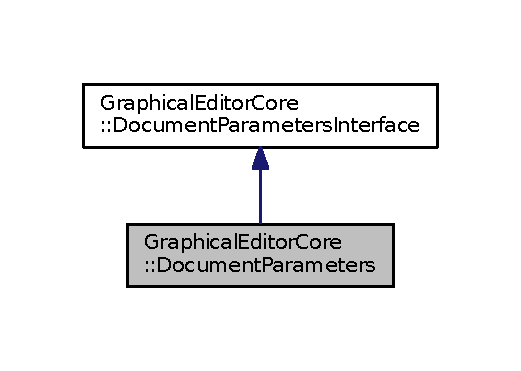
\includegraphics[width=250pt]{classGraphicalEditorCore_1_1DocumentParameters__inherit__graph}
\end{center}
\end{figure}


Collaboration diagram for Graphical\+Editor\+Core\+:\+:Document\+Parameters$<$ T $>$\+:
\nopagebreak
\begin{figure}[H]
\begin{center}
\leavevmode
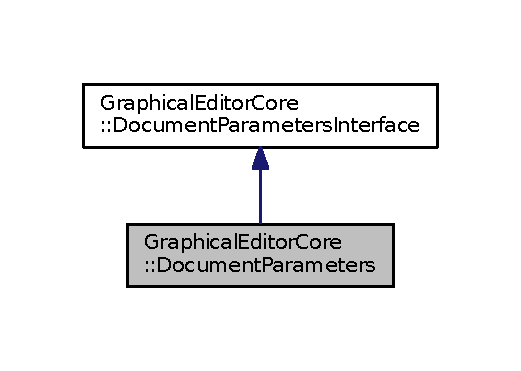
\includegraphics[width=250pt]{classGraphicalEditorCore_1_1DocumentParameters__coll__graph}
\end{center}
\end{figure}
\subsection*{Public Member Functions}
\begin{DoxyCompactItemize}
\item 
\hyperlink{classGraphicalEditorCore_1_1DocumentParameters_a2f886f265cbb7c548763142c05daa7f9}{Document\+Parameters} ()
\item 
\hyperlink{classGraphicalEditorCore_1_1DocumentParameters_af51920612aedf38f46b341b675f6f271}{Document\+Parameters} (const \hyperlink{classGraphicalEditorCore_1_1DocumentParameters}{Document\+Parameters} \&)
\item 
\hyperlink{classGraphicalEditorCore_1_1DocumentParameters_a3fc1cb785673903106dce2a4c6d47875}{Document\+Parameters} (\hyperlink{classGraphicalEditorCore_1_1DocumentParameters}{Document\+Parameters} \&\&)
\item 
\hyperlink{classGraphicalEditorCore_1_1DocumentParameters}{Document\+Parameters} \& \hyperlink{classGraphicalEditorCore_1_1DocumentParameters_ab4603c9baf2d76b9405fd099572546f4}{operator=} (const \hyperlink{classGraphicalEditorCore_1_1DocumentParameters}{Document\+Parameters} \&)
\item 
\hyperlink{classGraphicalEditorCore_1_1DocumentParameters}{Document\+Parameters} \& \hyperlink{classGraphicalEditorCore_1_1DocumentParameters_a635d305147d085a54281dd135601afa9}{operator=} (\hyperlink{classGraphicalEditorCore_1_1DocumentParameters}{Document\+Parameters} \&\&)
\item 
virtual \hyperlink{classGraphicalEditorCore_1_1DocumentParameters_a390ce6cb3be137d584bb7c74965325b7}{$\sim$\+Document\+Parameters} ()
\item 
virtual size\+\_\+t \hyperlink{classGraphicalEditorCore_1_1DocumentParameters_a96834b7081ba4001cf0c8a38532f3a48}{width} () const override
\item 
virtual size\+\_\+t \hyperlink{classGraphicalEditorCore_1_1DocumentParameters_ab1a929a3638767bbb361e9a7c69e9374}{height} () const override
\item 
virtual T \& \hyperlink{classGraphicalEditorCore_1_1DocumentParameters_a49010b1753c4a62a46bf01da20f17e61}{color\+Engine} () const override
\item 
virtual void \hyperlink{classGraphicalEditorCore_1_1DocumentParameters_a5970a79e783f85042786150e32fba8c5}{append} (\hyperlink{classGraphicalEditorCore_1_1DocumentWriterBase}{Document\+Writer\+Base} \&wr\+\_\+eng) override
\item 
void \hyperlink{classGraphicalEditorCore_1_1DocumentParameters_a1b982f66a9fd844c3ecbba465bf85ad1}{set\+Width} (const size\+\_\+t w)
\item 
void \hyperlink{classGraphicalEditorCore_1_1DocumentParameters_a399ffb889b05829955ed0ab4020408ef}{set\+Height} (const size\+\_\+t h)
\item 
void \hyperlink{classGraphicalEditorCore_1_1DocumentParameters_afdd4ea9fd33458fdfdb125b286a75344}{reset\+Color\+Engine} (T $\ast$const ptr\+\_\+clr\+\_\+eng)
\end{DoxyCompactItemize}


\subsection{Constructor \& Destructor Documentation}
\index{Graphical\+Editor\+Core\+::\+Document\+Parameters@{Graphical\+Editor\+Core\+::\+Document\+Parameters}!Document\+Parameters@{Document\+Parameters}}
\index{Document\+Parameters@{Document\+Parameters}!Graphical\+Editor\+Core\+::\+Document\+Parameters@{Graphical\+Editor\+Core\+::\+Document\+Parameters}}
\subsubsection[{\texorpdfstring{Document\+Parameters()}{DocumentParameters()}}]{\setlength{\rightskip}{0pt plus 5cm}template$<$typename T $>$ {\bf Graphical\+Editor\+Core\+::\+Document\+Parameters}$<$ T $>$\+::{\bf Document\+Parameters} (
\begin{DoxyParamCaption}
{}
\end{DoxyParamCaption}
)}\hypertarget{classGraphicalEditorCore_1_1DocumentParameters_a2f886f265cbb7c548763142c05daa7f9}{}\label{classGraphicalEditorCore_1_1DocumentParameters_a2f886f265cbb7c548763142c05daa7f9}
\index{Graphical\+Editor\+Core\+::\+Document\+Parameters@{Graphical\+Editor\+Core\+::\+Document\+Parameters}!Document\+Parameters@{Document\+Parameters}}
\index{Document\+Parameters@{Document\+Parameters}!Graphical\+Editor\+Core\+::\+Document\+Parameters@{Graphical\+Editor\+Core\+::\+Document\+Parameters}}
\subsubsection[{\texorpdfstring{Document\+Parameters(const Document\+Parameters \&)}{DocumentParameters(const DocumentParameters &)}}]{\setlength{\rightskip}{0pt plus 5cm}template$<$typename T $>$ {\bf Graphical\+Editor\+Core\+::\+Document\+Parameters}$<$ T $>$\+::{\bf Document\+Parameters} (
\begin{DoxyParamCaption}
\item[{const {\bf Document\+Parameters}$<$ T $>$ \&}]{rhs}
\end{DoxyParamCaption}
)}\hypertarget{classGraphicalEditorCore_1_1DocumentParameters_af51920612aedf38f46b341b675f6f271}{}\label{classGraphicalEditorCore_1_1DocumentParameters_af51920612aedf38f46b341b675f6f271}
\index{Graphical\+Editor\+Core\+::\+Document\+Parameters@{Graphical\+Editor\+Core\+::\+Document\+Parameters}!Document\+Parameters@{Document\+Parameters}}
\index{Document\+Parameters@{Document\+Parameters}!Graphical\+Editor\+Core\+::\+Document\+Parameters@{Graphical\+Editor\+Core\+::\+Document\+Parameters}}
\subsubsection[{\texorpdfstring{Document\+Parameters(\+Document\+Parameters \&\&)}{DocumentParameters(DocumentParameters &&)}}]{\setlength{\rightskip}{0pt plus 5cm}template$<$typename T $>$ {\bf Graphical\+Editor\+Core\+::\+Document\+Parameters}$<$ T $>$\+::{\bf Document\+Parameters} (
\begin{DoxyParamCaption}
\item[{{\bf Document\+Parameters}$<$ T $>$ \&\&}]{rhs}
\end{DoxyParamCaption}
)}\hypertarget{classGraphicalEditorCore_1_1DocumentParameters_a3fc1cb785673903106dce2a4c6d47875}{}\label{classGraphicalEditorCore_1_1DocumentParameters_a3fc1cb785673903106dce2a4c6d47875}
\index{Graphical\+Editor\+Core\+::\+Document\+Parameters@{Graphical\+Editor\+Core\+::\+Document\+Parameters}!````~Document\+Parameters@{$\sim$\+Document\+Parameters}}
\index{````~Document\+Parameters@{$\sim$\+Document\+Parameters}!Graphical\+Editor\+Core\+::\+Document\+Parameters@{Graphical\+Editor\+Core\+::\+Document\+Parameters}}
\subsubsection[{\texorpdfstring{$\sim$\+Document\+Parameters()}{~DocumentParameters()}}]{\setlength{\rightskip}{0pt plus 5cm}template$<$typename T $>$ {\bf Graphical\+Editor\+Core\+::\+Document\+Parameters}$<$ T $>$\+::$\sim${\bf Document\+Parameters} (
\begin{DoxyParamCaption}
{}
\end{DoxyParamCaption}
)\hspace{0.3cm}{\ttfamily [virtual]}}\hypertarget{classGraphicalEditorCore_1_1DocumentParameters_a390ce6cb3be137d584bb7c74965325b7}{}\label{classGraphicalEditorCore_1_1DocumentParameters_a390ce6cb3be137d584bb7c74965325b7}


\subsection{Member Function Documentation}
\index{Graphical\+Editor\+Core\+::\+Document\+Parameters@{Graphical\+Editor\+Core\+::\+Document\+Parameters}!append@{append}}
\index{append@{append}!Graphical\+Editor\+Core\+::\+Document\+Parameters@{Graphical\+Editor\+Core\+::\+Document\+Parameters}}
\subsubsection[{\texorpdfstring{append(\+Document\+Writer\+Base \&wr\+\_\+eng) override}{append(DocumentWriterBase &wr_eng) override}}]{\setlength{\rightskip}{0pt plus 5cm}template$<$typename T $>$ void {\bf Graphical\+Editor\+Core\+::\+Document\+Parameters}$<$ T $>$\+::append (
\begin{DoxyParamCaption}
\item[{{\bf Document\+Writer\+Base} \&}]{wr\+\_\+eng}
\end{DoxyParamCaption}
)\hspace{0.3cm}{\ttfamily [override]}, {\ttfamily [virtual]}}\hypertarget{classGraphicalEditorCore_1_1DocumentParameters_a5970a79e783f85042786150e32fba8c5}{}\label{classGraphicalEditorCore_1_1DocumentParameters_a5970a79e783f85042786150e32fba8c5}


Implements \hyperlink{classGraphicalEditorCore_1_1DocumentParametersInterface_a0f00de40222b9f5176e2cf6d4e9ae4c9}{Graphical\+Editor\+Core\+::\+Document\+Parameters\+Interface}.

\index{Graphical\+Editor\+Core\+::\+Document\+Parameters@{Graphical\+Editor\+Core\+::\+Document\+Parameters}!color\+Engine@{color\+Engine}}
\index{color\+Engine@{color\+Engine}!Graphical\+Editor\+Core\+::\+Document\+Parameters@{Graphical\+Editor\+Core\+::\+Document\+Parameters}}
\subsubsection[{\texorpdfstring{color\+Engine() const override}{colorEngine() const override}}]{\setlength{\rightskip}{0pt plus 5cm}template$<$typename T $>$ T \& {\bf Graphical\+Editor\+Core\+::\+Document\+Parameters}$<$ T $>$\+::color\+Engine (
\begin{DoxyParamCaption}
{}
\end{DoxyParamCaption}
) const\hspace{0.3cm}{\ttfamily [override]}, {\ttfamily [virtual]}}\hypertarget{classGraphicalEditorCore_1_1DocumentParameters_a49010b1753c4a62a46bf01da20f17e61}{}\label{classGraphicalEditorCore_1_1DocumentParameters_a49010b1753c4a62a46bf01da20f17e61}


Implements \hyperlink{classGraphicalEditorCore_1_1DocumentParametersInterface_aa686512ed2fc7bc504c1ee97ac8e4ad6}{Graphical\+Editor\+Core\+::\+Document\+Parameters\+Interface}.

\index{Graphical\+Editor\+Core\+::\+Document\+Parameters@{Graphical\+Editor\+Core\+::\+Document\+Parameters}!height@{height}}
\index{height@{height}!Graphical\+Editor\+Core\+::\+Document\+Parameters@{Graphical\+Editor\+Core\+::\+Document\+Parameters}}
\subsubsection[{\texorpdfstring{height() const override}{height() const override}}]{\setlength{\rightskip}{0pt plus 5cm}template$<$typename T $>$ size\+\_\+t {\bf Graphical\+Editor\+Core\+::\+Document\+Parameters}$<$ T $>$\+::height (
\begin{DoxyParamCaption}
{}
\end{DoxyParamCaption}
) const\hspace{0.3cm}{\ttfamily [override]}, {\ttfamily [virtual]}}\hypertarget{classGraphicalEditorCore_1_1DocumentParameters_ab1a929a3638767bbb361e9a7c69e9374}{}\label{classGraphicalEditorCore_1_1DocumentParameters_ab1a929a3638767bbb361e9a7c69e9374}


Implements \hyperlink{classGraphicalEditorCore_1_1DocumentParametersInterface_a1a3f45e27f2c9b11d04b2fe562323bb2}{Graphical\+Editor\+Core\+::\+Document\+Parameters\+Interface}.

\index{Graphical\+Editor\+Core\+::\+Document\+Parameters@{Graphical\+Editor\+Core\+::\+Document\+Parameters}!operator=@{operator=}}
\index{operator=@{operator=}!Graphical\+Editor\+Core\+::\+Document\+Parameters@{Graphical\+Editor\+Core\+::\+Document\+Parameters}}
\subsubsection[{\texorpdfstring{operator=(const Document\+Parameters \&)}{operator=(const DocumentParameters &)}}]{\setlength{\rightskip}{0pt plus 5cm}template$<$typename T $>$ {\bf Document\+Parameters}$<$ T $>$ \& {\bf Graphical\+Editor\+Core\+::\+Document\+Parameters}$<$ T $>$\+::operator= (
\begin{DoxyParamCaption}
\item[{const {\bf Document\+Parameters}$<$ T $>$ \&}]{rhs}
\end{DoxyParamCaption}
)}\hypertarget{classGraphicalEditorCore_1_1DocumentParameters_ab4603c9baf2d76b9405fd099572546f4}{}\label{classGraphicalEditorCore_1_1DocumentParameters_ab4603c9baf2d76b9405fd099572546f4}
\index{Graphical\+Editor\+Core\+::\+Document\+Parameters@{Graphical\+Editor\+Core\+::\+Document\+Parameters}!operator=@{operator=}}
\index{operator=@{operator=}!Graphical\+Editor\+Core\+::\+Document\+Parameters@{Graphical\+Editor\+Core\+::\+Document\+Parameters}}
\subsubsection[{\texorpdfstring{operator=(\+Document\+Parameters \&\&)}{operator=(DocumentParameters &&)}}]{\setlength{\rightskip}{0pt plus 5cm}template$<$typename T $>$ {\bf Document\+Parameters}$<$ T $>$ \& {\bf Graphical\+Editor\+Core\+::\+Document\+Parameters}$<$ T $>$\+::operator= (
\begin{DoxyParamCaption}
\item[{{\bf Document\+Parameters}$<$ T $>$ \&\&}]{rhs}
\end{DoxyParamCaption}
)}\hypertarget{classGraphicalEditorCore_1_1DocumentParameters_a635d305147d085a54281dd135601afa9}{}\label{classGraphicalEditorCore_1_1DocumentParameters_a635d305147d085a54281dd135601afa9}
\index{Graphical\+Editor\+Core\+::\+Document\+Parameters@{Graphical\+Editor\+Core\+::\+Document\+Parameters}!reset\+Color\+Engine@{reset\+Color\+Engine}}
\index{reset\+Color\+Engine@{reset\+Color\+Engine}!Graphical\+Editor\+Core\+::\+Document\+Parameters@{Graphical\+Editor\+Core\+::\+Document\+Parameters}}
\subsubsection[{\texorpdfstring{reset\+Color\+Engine(\+T $\ast$const ptr\+\_\+clr\+\_\+eng)}{resetColorEngine(T *const ptr_clr_eng)}}]{\setlength{\rightskip}{0pt plus 5cm}template$<$typename T $>$ void {\bf Graphical\+Editor\+Core\+::\+Document\+Parameters}$<$ T $>$\+::reset\+Color\+Engine (
\begin{DoxyParamCaption}
\item[{T $\ast$const}]{ptr\+\_\+clr\+\_\+eng}
\end{DoxyParamCaption}
)}\hypertarget{classGraphicalEditorCore_1_1DocumentParameters_afdd4ea9fd33458fdfdb125b286a75344}{}\label{classGraphicalEditorCore_1_1DocumentParameters_afdd4ea9fd33458fdfdb125b286a75344}
\index{Graphical\+Editor\+Core\+::\+Document\+Parameters@{Graphical\+Editor\+Core\+::\+Document\+Parameters}!set\+Height@{set\+Height}}
\index{set\+Height@{set\+Height}!Graphical\+Editor\+Core\+::\+Document\+Parameters@{Graphical\+Editor\+Core\+::\+Document\+Parameters}}
\subsubsection[{\texorpdfstring{set\+Height(const size\+\_\+t h)}{setHeight(const size_t h)}}]{\setlength{\rightskip}{0pt plus 5cm}template$<$typename T $>$ void {\bf Graphical\+Editor\+Core\+::\+Document\+Parameters}$<$ T $>$\+::set\+Height (
\begin{DoxyParamCaption}
\item[{const size\+\_\+t}]{h}
\end{DoxyParamCaption}
)}\hypertarget{classGraphicalEditorCore_1_1DocumentParameters_a399ffb889b05829955ed0ab4020408ef}{}\label{classGraphicalEditorCore_1_1DocumentParameters_a399ffb889b05829955ed0ab4020408ef}
\index{Graphical\+Editor\+Core\+::\+Document\+Parameters@{Graphical\+Editor\+Core\+::\+Document\+Parameters}!set\+Width@{set\+Width}}
\index{set\+Width@{set\+Width}!Graphical\+Editor\+Core\+::\+Document\+Parameters@{Graphical\+Editor\+Core\+::\+Document\+Parameters}}
\subsubsection[{\texorpdfstring{set\+Width(const size\+\_\+t w)}{setWidth(const size_t w)}}]{\setlength{\rightskip}{0pt plus 5cm}template$<$typename T $>$ void {\bf Graphical\+Editor\+Core\+::\+Document\+Parameters}$<$ T $>$\+::set\+Width (
\begin{DoxyParamCaption}
\item[{const size\+\_\+t}]{w}
\end{DoxyParamCaption}
)}\hypertarget{classGraphicalEditorCore_1_1DocumentParameters_a1b982f66a9fd844c3ecbba465bf85ad1}{}\label{classGraphicalEditorCore_1_1DocumentParameters_a1b982f66a9fd844c3ecbba465bf85ad1}
\index{Graphical\+Editor\+Core\+::\+Document\+Parameters@{Graphical\+Editor\+Core\+::\+Document\+Parameters}!width@{width}}
\index{width@{width}!Graphical\+Editor\+Core\+::\+Document\+Parameters@{Graphical\+Editor\+Core\+::\+Document\+Parameters}}
\subsubsection[{\texorpdfstring{width() const override}{width() const override}}]{\setlength{\rightskip}{0pt plus 5cm}template$<$typename T $>$ size\+\_\+t {\bf Graphical\+Editor\+Core\+::\+Document\+Parameters}$<$ T $>$\+::width (
\begin{DoxyParamCaption}
{}
\end{DoxyParamCaption}
) const\hspace{0.3cm}{\ttfamily [override]}, {\ttfamily [virtual]}}\hypertarget{classGraphicalEditorCore_1_1DocumentParameters_a96834b7081ba4001cf0c8a38532f3a48}{}\label{classGraphicalEditorCore_1_1DocumentParameters_a96834b7081ba4001cf0c8a38532f3a48}


Implements \hyperlink{classGraphicalEditorCore_1_1DocumentParametersInterface_a8e96d1aa50d0b2bd3ef21fafaeaa4261}{Graphical\+Editor\+Core\+::\+Document\+Parameters\+Interface}.



The documentation for this class was generated from the following files\+:\begin{DoxyCompactItemize}
\item 
05\+\_\+editor/\hyperlink{document__parameters_8h}{document\+\_\+parameters.\+h}\item 
05\+\_\+editor/\hyperlink{document__parameters_8cpp}{document\+\_\+parameters.\+cpp}\end{DoxyCompactItemize}

\hypertarget{classGraphicalEditorCore_1_1DocumentParametersInterface}{}\section{Graphical\+Editor\+Core\+:\+:Document\+Parameters\+Interface Class Reference}
\label{classGraphicalEditorCore_1_1DocumentParametersInterface}\index{Graphical\+Editor\+Core\+::\+Document\+Parameters\+Interface@{Graphical\+Editor\+Core\+::\+Document\+Parameters\+Interface}}


{\ttfamily \#include $<$document\+\_\+parameters.\+h$>$}



Inheritance diagram for Graphical\+Editor\+Core\+:\+:Document\+Parameters\+Interface\+:
\nopagebreak
\begin{figure}[H]
\begin{center}
\leavevmode
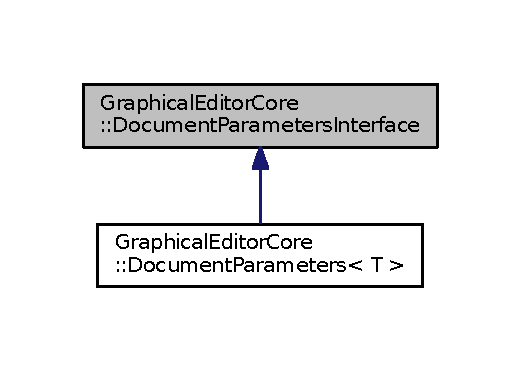
\includegraphics[width=250pt]{classGraphicalEditorCore_1_1DocumentParametersInterface__inherit__graph}
\end{center}
\end{figure}
\subsection*{Public Member Functions}
\begin{DoxyCompactItemize}
\item 
\hyperlink{classGraphicalEditorCore_1_1DocumentParametersInterface_aea8d5f5d01c0046d0bc2adad22487b23}{Document\+Parameters\+Interface} ()=default
\item 
\hyperlink{classGraphicalEditorCore_1_1DocumentParametersInterface_a95795d8f0e1cb69c18b468739325a0bb}{Document\+Parameters\+Interface} (const \hyperlink{classGraphicalEditorCore_1_1DocumentParametersInterface}{Document\+Parameters\+Interface} \&)=default
\item 
\hyperlink{classGraphicalEditorCore_1_1DocumentParametersInterface_a72b15c164f9f457c29d314ba6762fd84}{Document\+Parameters\+Interface} (\hyperlink{classGraphicalEditorCore_1_1DocumentParametersInterface}{Document\+Parameters\+Interface} \&\&)=default
\item 
\hyperlink{classGraphicalEditorCore_1_1DocumentParametersInterface}{Document\+Parameters\+Interface} \& \hyperlink{classGraphicalEditorCore_1_1DocumentParametersInterface_aa5a6d4d881b9812f8406f01ec1e20e50}{operator=} (const \hyperlink{classGraphicalEditorCore_1_1DocumentParametersInterface}{Document\+Parameters\+Interface} \&)=default
\item 
\hyperlink{classGraphicalEditorCore_1_1DocumentParametersInterface}{Document\+Parameters\+Interface} \& \hyperlink{classGraphicalEditorCore_1_1DocumentParametersInterface_a43e956fc79f52aff91ea8e2d0b952e5c}{operator=} (\hyperlink{classGraphicalEditorCore_1_1DocumentParametersInterface}{Document\+Parameters\+Interface} \&\&)=default
\item 
virtual \hyperlink{classGraphicalEditorCore_1_1DocumentParametersInterface_a17f379e6cde775c74283e90d046372e4}{$\sim$\+Document\+Parameters\+Interface} ()=default
\item 
virtual size\+\_\+t \hyperlink{classGraphicalEditorCore_1_1DocumentParametersInterface_a8e96d1aa50d0b2bd3ef21fafaeaa4261}{width} () const =0
\item 
virtual size\+\_\+t \hyperlink{classGraphicalEditorCore_1_1DocumentParametersInterface_a1a3f45e27f2c9b11d04b2fe562323bb2}{height} () const =0
\end{DoxyCompactItemize}


\subsection{Constructor \& Destructor Documentation}
\index{Graphical\+Editor\+Core\+::\+Document\+Parameters\+Interface@{Graphical\+Editor\+Core\+::\+Document\+Parameters\+Interface}!Document\+Parameters\+Interface@{Document\+Parameters\+Interface}}
\index{Document\+Parameters\+Interface@{Document\+Parameters\+Interface}!Graphical\+Editor\+Core\+::\+Document\+Parameters\+Interface@{Graphical\+Editor\+Core\+::\+Document\+Parameters\+Interface}}
\subsubsection[{\texorpdfstring{Document\+Parameters\+Interface()=default}{DocumentParametersInterface()=default}}]{\setlength{\rightskip}{0pt plus 5cm}Graphical\+Editor\+Core\+::\+Document\+Parameters\+Interface\+::\+Document\+Parameters\+Interface (
\begin{DoxyParamCaption}
{}
\end{DoxyParamCaption}
)\hspace{0.3cm}{\ttfamily [default]}}\hypertarget{classGraphicalEditorCore_1_1DocumentParametersInterface_aea8d5f5d01c0046d0bc2adad22487b23}{}\label{classGraphicalEditorCore_1_1DocumentParametersInterface_aea8d5f5d01c0046d0bc2adad22487b23}
\index{Graphical\+Editor\+Core\+::\+Document\+Parameters\+Interface@{Graphical\+Editor\+Core\+::\+Document\+Parameters\+Interface}!Document\+Parameters\+Interface@{Document\+Parameters\+Interface}}
\index{Document\+Parameters\+Interface@{Document\+Parameters\+Interface}!Graphical\+Editor\+Core\+::\+Document\+Parameters\+Interface@{Graphical\+Editor\+Core\+::\+Document\+Parameters\+Interface}}
\subsubsection[{\texorpdfstring{Document\+Parameters\+Interface(const Document\+Parameters\+Interface \&)=default}{DocumentParametersInterface(const DocumentParametersInterface &)=default}}]{\setlength{\rightskip}{0pt plus 5cm}Graphical\+Editor\+Core\+::\+Document\+Parameters\+Interface\+::\+Document\+Parameters\+Interface (
\begin{DoxyParamCaption}
\item[{const {\bf Document\+Parameters\+Interface} \&}]{}
\end{DoxyParamCaption}
)\hspace{0.3cm}{\ttfamily [default]}}\hypertarget{classGraphicalEditorCore_1_1DocumentParametersInterface_a95795d8f0e1cb69c18b468739325a0bb}{}\label{classGraphicalEditorCore_1_1DocumentParametersInterface_a95795d8f0e1cb69c18b468739325a0bb}
\index{Graphical\+Editor\+Core\+::\+Document\+Parameters\+Interface@{Graphical\+Editor\+Core\+::\+Document\+Parameters\+Interface}!Document\+Parameters\+Interface@{Document\+Parameters\+Interface}}
\index{Document\+Parameters\+Interface@{Document\+Parameters\+Interface}!Graphical\+Editor\+Core\+::\+Document\+Parameters\+Interface@{Graphical\+Editor\+Core\+::\+Document\+Parameters\+Interface}}
\subsubsection[{\texorpdfstring{Document\+Parameters\+Interface(\+Document\+Parameters\+Interface \&\&)=default}{DocumentParametersInterface(DocumentParametersInterface &&)=default}}]{\setlength{\rightskip}{0pt plus 5cm}Graphical\+Editor\+Core\+::\+Document\+Parameters\+Interface\+::\+Document\+Parameters\+Interface (
\begin{DoxyParamCaption}
\item[{{\bf Document\+Parameters\+Interface} \&\&}]{}
\end{DoxyParamCaption}
)\hspace{0.3cm}{\ttfamily [default]}}\hypertarget{classGraphicalEditorCore_1_1DocumentParametersInterface_a72b15c164f9f457c29d314ba6762fd84}{}\label{classGraphicalEditorCore_1_1DocumentParametersInterface_a72b15c164f9f457c29d314ba6762fd84}
\index{Graphical\+Editor\+Core\+::\+Document\+Parameters\+Interface@{Graphical\+Editor\+Core\+::\+Document\+Parameters\+Interface}!````~Document\+Parameters\+Interface@{$\sim$\+Document\+Parameters\+Interface}}
\index{````~Document\+Parameters\+Interface@{$\sim$\+Document\+Parameters\+Interface}!Graphical\+Editor\+Core\+::\+Document\+Parameters\+Interface@{Graphical\+Editor\+Core\+::\+Document\+Parameters\+Interface}}
\subsubsection[{\texorpdfstring{$\sim$\+Document\+Parameters\+Interface()=default}{~DocumentParametersInterface()=default}}]{\setlength{\rightskip}{0pt plus 5cm}virtual Graphical\+Editor\+Core\+::\+Document\+Parameters\+Interface\+::$\sim$\+Document\+Parameters\+Interface (
\begin{DoxyParamCaption}
{}
\end{DoxyParamCaption}
)\hspace{0.3cm}{\ttfamily [virtual]}, {\ttfamily [default]}}\hypertarget{classGraphicalEditorCore_1_1DocumentParametersInterface_a17f379e6cde775c74283e90d046372e4}{}\label{classGraphicalEditorCore_1_1DocumentParametersInterface_a17f379e6cde775c74283e90d046372e4}


\subsection{Member Function Documentation}
\index{Graphical\+Editor\+Core\+::\+Document\+Parameters\+Interface@{Graphical\+Editor\+Core\+::\+Document\+Parameters\+Interface}!height@{height}}
\index{height@{height}!Graphical\+Editor\+Core\+::\+Document\+Parameters\+Interface@{Graphical\+Editor\+Core\+::\+Document\+Parameters\+Interface}}
\subsubsection[{\texorpdfstring{height() const =0}{height() const =0}}]{\setlength{\rightskip}{0pt plus 5cm}virtual size\+\_\+t Graphical\+Editor\+Core\+::\+Document\+Parameters\+Interface\+::height (
\begin{DoxyParamCaption}
{}
\end{DoxyParamCaption}
) const\hspace{0.3cm}{\ttfamily [pure virtual]}}\hypertarget{classGraphicalEditorCore_1_1DocumentParametersInterface_a1a3f45e27f2c9b11d04b2fe562323bb2}{}\label{classGraphicalEditorCore_1_1DocumentParametersInterface_a1a3f45e27f2c9b11d04b2fe562323bb2}


Implemented in \hyperlink{classGraphicalEditorCore_1_1DocumentParameters_ab28b51581bade5d1b1a4122b347995da}{Graphical\+Editor\+Core\+::\+Document\+Parameters}.

\index{Graphical\+Editor\+Core\+::\+Document\+Parameters\+Interface@{Graphical\+Editor\+Core\+::\+Document\+Parameters\+Interface}!operator=@{operator=}}
\index{operator=@{operator=}!Graphical\+Editor\+Core\+::\+Document\+Parameters\+Interface@{Graphical\+Editor\+Core\+::\+Document\+Parameters\+Interface}}
\subsubsection[{\texorpdfstring{operator=(const Document\+Parameters\+Interface \&)=default}{operator=(const DocumentParametersInterface &)=default}}]{\setlength{\rightskip}{0pt plus 5cm}{\bf Document\+Parameters\+Interface}\& Graphical\+Editor\+Core\+::\+Document\+Parameters\+Interface\+::operator= (
\begin{DoxyParamCaption}
\item[{const {\bf Document\+Parameters\+Interface} \&}]{}
\end{DoxyParamCaption}
)\hspace{0.3cm}{\ttfamily [default]}}\hypertarget{classGraphicalEditorCore_1_1DocumentParametersInterface_aa5a6d4d881b9812f8406f01ec1e20e50}{}\label{classGraphicalEditorCore_1_1DocumentParametersInterface_aa5a6d4d881b9812f8406f01ec1e20e50}
\index{Graphical\+Editor\+Core\+::\+Document\+Parameters\+Interface@{Graphical\+Editor\+Core\+::\+Document\+Parameters\+Interface}!operator=@{operator=}}
\index{operator=@{operator=}!Graphical\+Editor\+Core\+::\+Document\+Parameters\+Interface@{Graphical\+Editor\+Core\+::\+Document\+Parameters\+Interface}}
\subsubsection[{\texorpdfstring{operator=(\+Document\+Parameters\+Interface \&\&)=default}{operator=(DocumentParametersInterface &&)=default}}]{\setlength{\rightskip}{0pt plus 5cm}{\bf Document\+Parameters\+Interface}\& Graphical\+Editor\+Core\+::\+Document\+Parameters\+Interface\+::operator= (
\begin{DoxyParamCaption}
\item[{{\bf Document\+Parameters\+Interface} \&\&}]{}
\end{DoxyParamCaption}
)\hspace{0.3cm}{\ttfamily [default]}}\hypertarget{classGraphicalEditorCore_1_1DocumentParametersInterface_a43e956fc79f52aff91ea8e2d0b952e5c}{}\label{classGraphicalEditorCore_1_1DocumentParametersInterface_a43e956fc79f52aff91ea8e2d0b952e5c}
\index{Graphical\+Editor\+Core\+::\+Document\+Parameters\+Interface@{Graphical\+Editor\+Core\+::\+Document\+Parameters\+Interface}!width@{width}}
\index{width@{width}!Graphical\+Editor\+Core\+::\+Document\+Parameters\+Interface@{Graphical\+Editor\+Core\+::\+Document\+Parameters\+Interface}}
\subsubsection[{\texorpdfstring{width() const =0}{width() const =0}}]{\setlength{\rightskip}{0pt plus 5cm}virtual size\+\_\+t Graphical\+Editor\+Core\+::\+Document\+Parameters\+Interface\+::width (
\begin{DoxyParamCaption}
{}
\end{DoxyParamCaption}
) const\hspace{0.3cm}{\ttfamily [pure virtual]}}\hypertarget{classGraphicalEditorCore_1_1DocumentParametersInterface_a8e96d1aa50d0b2bd3ef21fafaeaa4261}{}\label{classGraphicalEditorCore_1_1DocumentParametersInterface_a8e96d1aa50d0b2bd3ef21fafaeaa4261}


Implemented in \hyperlink{classGraphicalEditorCore_1_1DocumentParameters_af84100459d1e49474e57e5b7b16f1750}{Graphical\+Editor\+Core\+::\+Document\+Parameters}.



The documentation for this class was generated from the following file\+:\begin{DoxyCompactItemize}
\item 
05\+\_\+editor/\hyperlink{document__parameters_8h}{document\+\_\+parameters.\+h}\end{DoxyCompactItemize}

\hypertarget{classGraphicalEditorCore_1_1EditorCore}{}\section{Graphical\+Editor\+Core\+:\+:Editor\+Core$<$ T $>$ Class Template Reference}
\label{classGraphicalEditorCore_1_1EditorCore}\index{Graphical\+Editor\+Core\+::\+Editor\+Core$<$ T $>$@{Graphical\+Editor\+Core\+::\+Editor\+Core$<$ T $>$}}


{\ttfamily \#include $<$editor\+\_\+core.\+h$>$}

\subsection*{Public Member Functions}
\begin{DoxyCompactItemize}
\item 
\hyperlink{classGraphicalEditorCore_1_1EditorCore_ae6b7d39c0e657e2364d0e78bb2ada3ea}{Editor\+Core} ()
\item 
virtual \hyperlink{classGraphicalEditorCore_1_1EditorCore_ac16fa9bd735820ff6fbf3066dd271e81}{$\sim$\+Editor\+Core} ()
\item 
\hyperlink{classGraphicalEditorCore_1_1Document}{Document}$<$ T $>$ \& \hyperlink{classGraphicalEditorCore_1_1EditorCore_a4387885d89e2cf6e3cfdc255255c3047}{create\+\_\+document} (std\+::shared\+\_\+ptr$<$ \hyperlink{classGraphicalEditorCore_1_1DocumentParametersInterface}{Document\+Parameters\+Interface} $>$ shp\+\_\+dpi)
\item 
void \hyperlink{classGraphicalEditorCore_1_1EditorCore_adb7b174b5c93890dfbfc955a36a2ee4f}{reset\+\_\+writer} (std\+::unique\+\_\+ptr$<$ \hyperlink{classGraphicalEditorCore_1_1DocumentWriterBase}{Document\+Writer\+Base} $>$ \&\&doc\+\_\+writer)
\item 
void \hyperlink{classGraphicalEditorCore_1_1EditorCore_ad04cc698d57b190d4f78f50210c88a36}{save} (const std\+::string \&file)
\end{DoxyCompactItemize}


\subsection{Constructor \& Destructor Documentation}
\index{Graphical\+Editor\+Core\+::\+Editor\+Core@{Graphical\+Editor\+Core\+::\+Editor\+Core}!Editor\+Core@{Editor\+Core}}
\index{Editor\+Core@{Editor\+Core}!Graphical\+Editor\+Core\+::\+Editor\+Core@{Graphical\+Editor\+Core\+::\+Editor\+Core}}
\subsubsection[{\texorpdfstring{Editor\+Core()}{EditorCore()}}]{\setlength{\rightskip}{0pt plus 5cm}template$<$typename T $>$ {\bf Graphical\+Editor\+Core\+::\+Editor\+Core}$<$ T $>$\+::{\bf Editor\+Core} (
\begin{DoxyParamCaption}
{}
\end{DoxyParamCaption}
)}\hypertarget{classGraphicalEditorCore_1_1EditorCore_ae6b7d39c0e657e2364d0e78bb2ada3ea}{}\label{classGraphicalEditorCore_1_1EditorCore_ae6b7d39c0e657e2364d0e78bb2ada3ea}
\index{Graphical\+Editor\+Core\+::\+Editor\+Core@{Graphical\+Editor\+Core\+::\+Editor\+Core}!````~Editor\+Core@{$\sim$\+Editor\+Core}}
\index{````~Editor\+Core@{$\sim$\+Editor\+Core}!Graphical\+Editor\+Core\+::\+Editor\+Core@{Graphical\+Editor\+Core\+::\+Editor\+Core}}
\subsubsection[{\texorpdfstring{$\sim$\+Editor\+Core()}{~EditorCore()}}]{\setlength{\rightskip}{0pt plus 5cm}template$<$typename T $>$ {\bf Graphical\+Editor\+Core\+::\+Editor\+Core}$<$ T $>$\+::$\sim${\bf Editor\+Core} (
\begin{DoxyParamCaption}
{}
\end{DoxyParamCaption}
)\hspace{0.3cm}{\ttfamily [virtual]}}\hypertarget{classGraphicalEditorCore_1_1EditorCore_ac16fa9bd735820ff6fbf3066dd271e81}{}\label{classGraphicalEditorCore_1_1EditorCore_ac16fa9bd735820ff6fbf3066dd271e81}


\subsection{Member Function Documentation}
\index{Graphical\+Editor\+Core\+::\+Editor\+Core@{Graphical\+Editor\+Core\+::\+Editor\+Core}!create\+\_\+document@{create\+\_\+document}}
\index{create\+\_\+document@{create\+\_\+document}!Graphical\+Editor\+Core\+::\+Editor\+Core@{Graphical\+Editor\+Core\+::\+Editor\+Core}}
\subsubsection[{\texorpdfstring{create\+\_\+document(std\+::shared\+\_\+ptr$<$ Document\+Parameters\+Interface $>$ shp\+\_\+dpi)}{create_document(std::shared_ptr< DocumentParametersInterface > shp_dpi)}}]{\setlength{\rightskip}{0pt plus 5cm}template$<$typename T $>$ {\bf Document}$<$ T $>$ \& {\bf Graphical\+Editor\+Core\+::\+Editor\+Core}$<$ T $>$\+::create\+\_\+document (
\begin{DoxyParamCaption}
\item[{std\+::shared\+\_\+ptr$<$ {\bf Document\+Parameters\+Interface} $>$}]{shp\+\_\+dpi}
\end{DoxyParamCaption}
)}\hypertarget{classGraphicalEditorCore_1_1EditorCore_a4387885d89e2cf6e3cfdc255255c3047}{}\label{classGraphicalEditorCore_1_1EditorCore_a4387885d89e2cf6e3cfdc255255c3047}
\index{Graphical\+Editor\+Core\+::\+Editor\+Core@{Graphical\+Editor\+Core\+::\+Editor\+Core}!reset\+\_\+writer@{reset\+\_\+writer}}
\index{reset\+\_\+writer@{reset\+\_\+writer}!Graphical\+Editor\+Core\+::\+Editor\+Core@{Graphical\+Editor\+Core\+::\+Editor\+Core}}
\subsubsection[{\texorpdfstring{reset\+\_\+writer(std\+::unique\+\_\+ptr$<$ Document\+Writer\+Base $>$ \&\&doc\+\_\+writer)}{reset_writer(std::unique_ptr< DocumentWriterBase > &&doc_writer)}}]{\setlength{\rightskip}{0pt plus 5cm}template$<$typename T $>$ void {\bf Graphical\+Editor\+Core\+::\+Editor\+Core}$<$ T $>$\+::reset\+\_\+writer (
\begin{DoxyParamCaption}
\item[{std\+::unique\+\_\+ptr$<$ {\bf Document\+Writer\+Base} $>$ \&\&}]{doc\+\_\+writer}
\end{DoxyParamCaption}
)}\hypertarget{classGraphicalEditorCore_1_1EditorCore_adb7b174b5c93890dfbfc955a36a2ee4f}{}\label{classGraphicalEditorCore_1_1EditorCore_adb7b174b5c93890dfbfc955a36a2ee4f}
\index{Graphical\+Editor\+Core\+::\+Editor\+Core@{Graphical\+Editor\+Core\+::\+Editor\+Core}!save@{save}}
\index{save@{save}!Graphical\+Editor\+Core\+::\+Editor\+Core@{Graphical\+Editor\+Core\+::\+Editor\+Core}}
\subsubsection[{\texorpdfstring{save(const std\+::string \&file)}{save(const std::string &file)}}]{\setlength{\rightskip}{0pt plus 5cm}template$<$typename T $>$ void {\bf Graphical\+Editor\+Core\+::\+Editor\+Core}$<$ T $>$\+::save (
\begin{DoxyParamCaption}
\item[{const std\+::string \&}]{file}
\end{DoxyParamCaption}
)}\hypertarget{classGraphicalEditorCore_1_1EditorCore_ad04cc698d57b190d4f78f50210c88a36}{}\label{classGraphicalEditorCore_1_1EditorCore_ad04cc698d57b190d4f78f50210c88a36}


The documentation for this class was generated from the following files\+:\begin{DoxyCompactItemize}
\item 
05\+\_\+editor/\hyperlink{editor__core_8h}{editor\+\_\+core.\+h}\item 
05\+\_\+editor/\hyperlink{editor__core_8cpp}{editor\+\_\+core.\+cpp}\end{DoxyCompactItemize}

\hypertarget{structelem__type__holder}{}\section{elem\+\_\+type\+\_\+holder$<$ size\+\_\+t, typename $>$ Struct Template Reference}
\label{structelem__type__holder}\index{elem\+\_\+type\+\_\+holder$<$ size\+\_\+t, typename $>$@{elem\+\_\+type\+\_\+holder$<$ size\+\_\+t, typename $>$}}


{\ttfamily \#include $<$cstm\+\_\+tuple.\+hpp$>$}



The documentation for this struct was generated from the following file\+:\begin{DoxyCompactItemize}
\item 
02\+\_\+tuple/\hyperlink{cstm__tuple_8hpp}{cstm\+\_\+tuple.\+hpp}\end{DoxyCompactItemize}

\hypertarget{structelem__type__holder_3_010_00_01custom__tuple_3_01T_00_01Ts_8_8_8_01_4_01_4}{}\section{elem\+\_\+type\+\_\+holder$<$ 0, custom\+\_\+tuple$<$ T, Ts... $>$ $>$ Struct Template Reference}
\label{structelem__type__holder_3_010_00_01custom__tuple_3_01T_00_01Ts_8_8_8_01_4_01_4}\index{elem\+\_\+type\+\_\+holder$<$ 0, custom\+\_\+tuple$<$ T, Ts... $>$ $>$@{elem\+\_\+type\+\_\+holder$<$ 0, custom\+\_\+tuple$<$ T, Ts... $>$ $>$}}


{\ttfamily \#include $<$cstm\+\_\+tuple.\+hpp$>$}

\subsection*{Public Types}
\begin{DoxyCompactItemize}
\item 
typedef T \hyperlink{structelem__type__holder_3_010_00_01custom__tuple_3_01T_00_01Ts_8_8_8_01_4_01_4_af978e6f8de071074a4c26f7450fa2636}{type}
\end{DoxyCompactItemize}


\subsection{Member Typedef Documentation}
\index{elem\+\_\+type\+\_\+holder$<$ 0, custom\+\_\+tuple$<$ T, Ts... $>$ $>$@{elem\+\_\+type\+\_\+holder$<$ 0, custom\+\_\+tuple$<$ T, Ts... $>$ $>$}!type@{type}}
\index{type@{type}!elem\+\_\+type\+\_\+holder$<$ 0, custom\+\_\+tuple$<$ T, Ts... $>$ $>$@{elem\+\_\+type\+\_\+holder$<$ 0, custom\+\_\+tuple$<$ T, Ts... $>$ $>$}}
\subsubsection[{\texorpdfstring{type}{type}}]{\setlength{\rightskip}{0pt plus 5cm}template$<$typename T , typename... Ts$>$ typedef T {\bf elem\+\_\+type\+\_\+holder}$<$ 0, {\bf custom\+\_\+tuple}$<$ T, Ts... $>$ $>$\+::{\bf type}}\hypertarget{structelem__type__holder_3_010_00_01custom__tuple_3_01T_00_01Ts_8_8_8_01_4_01_4_af978e6f8de071074a4c26f7450fa2636}{}\label{structelem__type__holder_3_010_00_01custom__tuple_3_01T_00_01Ts_8_8_8_01_4_01_4_af978e6f8de071074a4c26f7450fa2636}


The documentation for this struct was generated from the following file\+:\begin{DoxyCompactItemize}
\item 
02\+\_\+tuple/\hyperlink{cstm__tuple_8hpp}{cstm\+\_\+tuple.\+hpp}\end{DoxyCompactItemize}

\hypertarget{structelem__type__holder_3_01k_00_01custom__tuple_3_01T_00_01Ts_8_8_8_01_4_01_4}{}\section{elem\+\_\+type\+\_\+holder$<$ k, custom\+\_\+tuple$<$ T, Ts... $>$ $>$ Struct Template Reference}
\label{structelem__type__holder_3_01k_00_01custom__tuple_3_01T_00_01Ts_8_8_8_01_4_01_4}\index{elem\+\_\+type\+\_\+holder$<$ k, custom\+\_\+tuple$<$ T, Ts... $>$ $>$@{elem\+\_\+type\+\_\+holder$<$ k, custom\+\_\+tuple$<$ T, Ts... $>$ $>$}}


{\ttfamily \#include $<$cstm\+\_\+tuple.\+hpp$>$}

\subsection*{Public Types}
\begin{DoxyCompactItemize}
\item 
typedef \hyperlink{structelem__type__holder}{elem\+\_\+type\+\_\+holder}$<$ k-\/1, \hyperlink{structcustom__tuple}{custom\+\_\+tuple}$<$ Ts... $>$ $>$\+::\hyperlink{structelem__type__holder_3_01k_00_01custom__tuple_3_01T_00_01Ts_8_8_8_01_4_01_4_ab3b1bf71db4e249545297ee87ba43659}{type} \hyperlink{structelem__type__holder_3_01k_00_01custom__tuple_3_01T_00_01Ts_8_8_8_01_4_01_4_ab3b1bf71db4e249545297ee87ba43659}{type}
\end{DoxyCompactItemize}


\subsection{Member Typedef Documentation}
\index{elem\+\_\+type\+\_\+holder$<$ k, custom\+\_\+tuple$<$ T, Ts... $>$ $>$@{elem\+\_\+type\+\_\+holder$<$ k, custom\+\_\+tuple$<$ T, Ts... $>$ $>$}!type@{type}}
\index{type@{type}!elem\+\_\+type\+\_\+holder$<$ k, custom\+\_\+tuple$<$ T, Ts... $>$ $>$@{elem\+\_\+type\+\_\+holder$<$ k, custom\+\_\+tuple$<$ T, Ts... $>$ $>$}}
\subsubsection[{\texorpdfstring{type}{type}}]{\setlength{\rightskip}{0pt plus 5cm}template$<$size\+\_\+t k, typename T , typename... Ts$>$ typedef {\bf elem\+\_\+type\+\_\+holder}$<$k -\/ 1, {\bf custom\+\_\+tuple}$<$Ts ... $>$ $>$\+::{\bf type} {\bf elem\+\_\+type\+\_\+holder}$<$ k, {\bf custom\+\_\+tuple}$<$ T, Ts... $>$ $>$\+::{\bf type}}\hypertarget{structelem__type__holder_3_01k_00_01custom__tuple_3_01T_00_01Ts_8_8_8_01_4_01_4_ab3b1bf71db4e249545297ee87ba43659}{}\label{structelem__type__holder_3_01k_00_01custom__tuple_3_01T_00_01Ts_8_8_8_01_4_01_4_ab3b1bf71db4e249545297ee87ba43659}


The documentation for this struct was generated from the following file\+:\begin{DoxyCompactItemize}
\item 
02\+\_\+tuple/\hyperlink{cstm__tuple_8hpp}{cstm\+\_\+tuple.\+hpp}\end{DoxyCompactItemize}

\hypertarget{classelementwise__block__allocator}{}\section{elementwise\+\_\+block\+\_\+allocator$<$ T $>$ Class Template Reference}
\label{classelementwise__block__allocator}\index{elementwise\+\_\+block\+\_\+allocator$<$ T $>$@{elementwise\+\_\+block\+\_\+allocator$<$ T $>$}}


{\ttfamily \#include $<$flexible\+\_\+allocator.\+hpp$>$}

\subsection*{Public Types}
\begin{DoxyCompactItemize}
\item 
using \hyperlink{classelementwise__block__allocator_aa2cd647e579b49a8640c13ff73fef25b}{value\+\_\+type} = T
\item 
using \hyperlink{classelementwise__block__allocator_af41c83aed240eb55e53155abdd714ec6}{pointer} = T $\ast$
\item 
using \hyperlink{classelementwise__block__allocator_a9382f12bfa2ba50e989f2f84216f44f1}{const\+\_\+pointer} = const T $\ast$
\item 
using \hyperlink{classelementwise__block__allocator_a7bfdf1ff6d23bcd486ef3c6541f738f2}{reference} = T \&
\item 
using \hyperlink{classelementwise__block__allocator_af7d02fdeb779527f9cc8723f8cebc40b}{const\+\_\+reference} = const T \&
\item 
using \hyperlink{classelementwise__block__allocator_a5a93e8060385c80ebaa62ec6e1b0d37e}{size\+\_\+type} = std\+::size\+\_\+t
\end{DoxyCompactItemize}
\subsection*{Public Member Functions}
\begin{DoxyCompactItemize}
\item 
\hyperlink{classelementwise__block__allocator_a8175b2d3ec243bd30a24aab1da8d6433}{elementwise\+\_\+block\+\_\+allocator} ()
\item 
virtual \hyperlink{classelementwise__block__allocator_a00e784cf4d72a47d3afc7a61dc6db98e}{$\sim$elementwise\+\_\+block\+\_\+allocator} ()=default
\item 
T $\ast$ \hyperlink{classelementwise__block__allocator_a244160f3cdc30a5cbe992b001da86cae}{allocate} (const size\+\_\+t n)
\item 
void \hyperlink{classelementwise__block__allocator_add41be398fcb515fec16622ff41e5f0f}{deallocate} (T $\ast$ptr, const size\+\_\+t n)
\item 
{\footnotesize template$<$typename U , typename... Args$>$ }\\void \hyperlink{classelementwise__block__allocator_a4826c3a40b3d5d9be3ab42191817f216}{construct} (U $\ast$ptr, Args \&\&...args)
\item 
{\footnotesize template$<$typename U $>$ }\\void \hyperlink{classelementwise__block__allocator_ae4e94b11ffdc895aa80d9b5d9b7b0999}{destroy} (U $\ast$ptr)
\end{DoxyCompactItemize}


\subsection{Member Typedef Documentation}
\index{elementwise\+\_\+block\+\_\+allocator@{elementwise\+\_\+block\+\_\+allocator}!const\+\_\+pointer@{const\+\_\+pointer}}
\index{const\+\_\+pointer@{const\+\_\+pointer}!elementwise\+\_\+block\+\_\+allocator@{elementwise\+\_\+block\+\_\+allocator}}
\subsubsection[{\texorpdfstring{const\+\_\+pointer}{const_pointer}}]{\setlength{\rightskip}{0pt plus 5cm}template$<$typename T $>$ using {\bf elementwise\+\_\+block\+\_\+allocator}$<$ T $>$\+::{\bf const\+\_\+pointer} =  const T $\ast$}\hypertarget{classelementwise__block__allocator_a9382f12bfa2ba50e989f2f84216f44f1}{}\label{classelementwise__block__allocator_a9382f12bfa2ba50e989f2f84216f44f1}
\index{elementwise\+\_\+block\+\_\+allocator@{elementwise\+\_\+block\+\_\+allocator}!const\+\_\+reference@{const\+\_\+reference}}
\index{const\+\_\+reference@{const\+\_\+reference}!elementwise\+\_\+block\+\_\+allocator@{elementwise\+\_\+block\+\_\+allocator}}
\subsubsection[{\texorpdfstring{const\+\_\+reference}{const_reference}}]{\setlength{\rightskip}{0pt plus 5cm}template$<$typename T $>$ using {\bf elementwise\+\_\+block\+\_\+allocator}$<$ T $>$\+::{\bf const\+\_\+reference} =  const T \&}\hypertarget{classelementwise__block__allocator_af7d02fdeb779527f9cc8723f8cebc40b}{}\label{classelementwise__block__allocator_af7d02fdeb779527f9cc8723f8cebc40b}
\index{elementwise\+\_\+block\+\_\+allocator@{elementwise\+\_\+block\+\_\+allocator}!pointer@{pointer}}
\index{pointer@{pointer}!elementwise\+\_\+block\+\_\+allocator@{elementwise\+\_\+block\+\_\+allocator}}
\subsubsection[{\texorpdfstring{pointer}{pointer}}]{\setlength{\rightskip}{0pt plus 5cm}template$<$typename T $>$ using {\bf elementwise\+\_\+block\+\_\+allocator}$<$ T $>$\+::{\bf pointer} =  T $\ast$}\hypertarget{classelementwise__block__allocator_af41c83aed240eb55e53155abdd714ec6}{}\label{classelementwise__block__allocator_af41c83aed240eb55e53155abdd714ec6}
\index{elementwise\+\_\+block\+\_\+allocator@{elementwise\+\_\+block\+\_\+allocator}!reference@{reference}}
\index{reference@{reference}!elementwise\+\_\+block\+\_\+allocator@{elementwise\+\_\+block\+\_\+allocator}}
\subsubsection[{\texorpdfstring{reference}{reference}}]{\setlength{\rightskip}{0pt plus 5cm}template$<$typename T $>$ using {\bf elementwise\+\_\+block\+\_\+allocator}$<$ T $>$\+::{\bf reference} =  T \&}\hypertarget{classelementwise__block__allocator_a7bfdf1ff6d23bcd486ef3c6541f738f2}{}\label{classelementwise__block__allocator_a7bfdf1ff6d23bcd486ef3c6541f738f2}
\index{elementwise\+\_\+block\+\_\+allocator@{elementwise\+\_\+block\+\_\+allocator}!size\+\_\+type@{size\+\_\+type}}
\index{size\+\_\+type@{size\+\_\+type}!elementwise\+\_\+block\+\_\+allocator@{elementwise\+\_\+block\+\_\+allocator}}
\subsubsection[{\texorpdfstring{size\+\_\+type}{size_type}}]{\setlength{\rightskip}{0pt plus 5cm}template$<$typename T $>$ using {\bf elementwise\+\_\+block\+\_\+allocator}$<$ T $>$\+::{\bf size\+\_\+type} =  std\+::size\+\_\+t}\hypertarget{classelementwise__block__allocator_a5a93e8060385c80ebaa62ec6e1b0d37e}{}\label{classelementwise__block__allocator_a5a93e8060385c80ebaa62ec6e1b0d37e}
\index{elementwise\+\_\+block\+\_\+allocator@{elementwise\+\_\+block\+\_\+allocator}!value\+\_\+type@{value\+\_\+type}}
\index{value\+\_\+type@{value\+\_\+type}!elementwise\+\_\+block\+\_\+allocator@{elementwise\+\_\+block\+\_\+allocator}}
\subsubsection[{\texorpdfstring{value\+\_\+type}{value_type}}]{\setlength{\rightskip}{0pt plus 5cm}template$<$typename T $>$ using {\bf elementwise\+\_\+block\+\_\+allocator}$<$ T $>$\+::{\bf value\+\_\+type} =  T}\hypertarget{classelementwise__block__allocator_aa2cd647e579b49a8640c13ff73fef25b}{}\label{classelementwise__block__allocator_aa2cd647e579b49a8640c13ff73fef25b}


\subsection{Constructor \& Destructor Documentation}
\index{elementwise\+\_\+block\+\_\+allocator@{elementwise\+\_\+block\+\_\+allocator}!elementwise\+\_\+block\+\_\+allocator@{elementwise\+\_\+block\+\_\+allocator}}
\index{elementwise\+\_\+block\+\_\+allocator@{elementwise\+\_\+block\+\_\+allocator}!elementwise\+\_\+block\+\_\+allocator@{elementwise\+\_\+block\+\_\+allocator}}
\subsubsection[{\texorpdfstring{elementwise\+\_\+block\+\_\+allocator()}{elementwise_block_allocator()}}]{\setlength{\rightskip}{0pt plus 5cm}template$<$typename T $>$ {\bf elementwise\+\_\+block\+\_\+allocator}$<$ T $>$\+::{\bf elementwise\+\_\+block\+\_\+allocator} (
\begin{DoxyParamCaption}
{}
\end{DoxyParamCaption}
)}\hypertarget{classelementwise__block__allocator_a8175b2d3ec243bd30a24aab1da8d6433}{}\label{classelementwise__block__allocator_a8175b2d3ec243bd30a24aab1da8d6433}
\index{elementwise\+\_\+block\+\_\+allocator@{elementwise\+\_\+block\+\_\+allocator}!````~elementwise\+\_\+block\+\_\+allocator@{$\sim$elementwise\+\_\+block\+\_\+allocator}}
\index{````~elementwise\+\_\+block\+\_\+allocator@{$\sim$elementwise\+\_\+block\+\_\+allocator}!elementwise\+\_\+block\+\_\+allocator@{elementwise\+\_\+block\+\_\+allocator}}
\subsubsection[{\texorpdfstring{$\sim$elementwise\+\_\+block\+\_\+allocator()=default}{~elementwise_block_allocator()=default}}]{\setlength{\rightskip}{0pt plus 5cm}template$<$typename T $>$ virtual {\bf elementwise\+\_\+block\+\_\+allocator}$<$ T $>$\+::$\sim${\bf elementwise\+\_\+block\+\_\+allocator} (
\begin{DoxyParamCaption}
{}
\end{DoxyParamCaption}
)\hspace{0.3cm}{\ttfamily [virtual]}, {\ttfamily [default]}}\hypertarget{classelementwise__block__allocator_a00e784cf4d72a47d3afc7a61dc6db98e}{}\label{classelementwise__block__allocator_a00e784cf4d72a47d3afc7a61dc6db98e}


\subsection{Member Function Documentation}
\index{elementwise\+\_\+block\+\_\+allocator@{elementwise\+\_\+block\+\_\+allocator}!allocate@{allocate}}
\index{allocate@{allocate}!elementwise\+\_\+block\+\_\+allocator@{elementwise\+\_\+block\+\_\+allocator}}
\subsubsection[{\texorpdfstring{allocate(const size\+\_\+t n)}{allocate(const size_t n)}}]{\setlength{\rightskip}{0pt plus 5cm}template$<$typename T $>$ T $\ast$ {\bf elementwise\+\_\+block\+\_\+allocator}$<$ T $>$\+::allocate (
\begin{DoxyParamCaption}
\item[{const size\+\_\+t}]{n}
\end{DoxyParamCaption}
)}\hypertarget{classelementwise__block__allocator_a244160f3cdc30a5cbe992b001da86cae}{}\label{classelementwise__block__allocator_a244160f3cdc30a5cbe992b001da86cae}
\index{elementwise\+\_\+block\+\_\+allocator@{elementwise\+\_\+block\+\_\+allocator}!construct@{construct}}
\index{construct@{construct}!elementwise\+\_\+block\+\_\+allocator@{elementwise\+\_\+block\+\_\+allocator}}
\subsubsection[{\texorpdfstring{construct(\+U $\ast$ptr, Args \&\&...\+args)}{construct(U *ptr, Args &&...args)}}]{\setlength{\rightskip}{0pt plus 5cm}template$<$typename T $>$ template$<$typename U , typename... Args$>$ void {\bf elementwise\+\_\+block\+\_\+allocator}$<$ T $>$\+::construct (
\begin{DoxyParamCaption}
\item[{U $\ast$}]{ptr, }
\item[{Args \&\&...}]{args}
\end{DoxyParamCaption}
)}\hypertarget{classelementwise__block__allocator_a4826c3a40b3d5d9be3ab42191817f216}{}\label{classelementwise__block__allocator_a4826c3a40b3d5d9be3ab42191817f216}
\index{elementwise\+\_\+block\+\_\+allocator@{elementwise\+\_\+block\+\_\+allocator}!deallocate@{deallocate}}
\index{deallocate@{deallocate}!elementwise\+\_\+block\+\_\+allocator@{elementwise\+\_\+block\+\_\+allocator}}
\subsubsection[{\texorpdfstring{deallocate(\+T $\ast$ptr, const size\+\_\+t n)}{deallocate(T *ptr, const size_t n)}}]{\setlength{\rightskip}{0pt plus 5cm}template$<$typename T $>$ void {\bf elementwise\+\_\+block\+\_\+allocator}$<$ T $>$\+::deallocate (
\begin{DoxyParamCaption}
\item[{T $\ast$}]{ptr, }
\item[{const size\+\_\+t}]{n}
\end{DoxyParamCaption}
)}\hypertarget{classelementwise__block__allocator_add41be398fcb515fec16622ff41e5f0f}{}\label{classelementwise__block__allocator_add41be398fcb515fec16622ff41e5f0f}
\index{elementwise\+\_\+block\+\_\+allocator@{elementwise\+\_\+block\+\_\+allocator}!destroy@{destroy}}
\index{destroy@{destroy}!elementwise\+\_\+block\+\_\+allocator@{elementwise\+\_\+block\+\_\+allocator}}
\subsubsection[{\texorpdfstring{destroy(\+U $\ast$ptr)}{destroy(U *ptr)}}]{\setlength{\rightskip}{0pt plus 5cm}template$<$typename T $>$ template$<$typename U $>$ void {\bf elementwise\+\_\+block\+\_\+allocator}$<$ T $>$\+::destroy (
\begin{DoxyParamCaption}
\item[{U $\ast$}]{ptr}
\end{DoxyParamCaption}
)}\hypertarget{classelementwise__block__allocator_ae4e94b11ffdc895aa80d9b5d9b7b0999}{}\label{classelementwise__block__allocator_ae4e94b11ffdc895aa80d9b5d9b7b0999}


The documentation for this class was generated from the following file\+:\begin{DoxyCompactItemize}
\item 
03\+\_\+allocator/\hyperlink{flexible__allocator_8hpp}{flexible\+\_\+allocator.\+hpp}\end{DoxyCompactItemize}

\hypertarget{classInfiniteMatrix}{}\section{Infinite\+Matrix$<$ T, Default\+Value $>$ Class Template Reference}
\label{classInfiniteMatrix}\index{Infinite\+Matrix$<$ T, Default\+Value $>$@{Infinite\+Matrix$<$ T, Default\+Value $>$}}


{\ttfamily \#include $<$infinite\+\_\+matrix.\+h$>$}

\subsection*{Public Member Functions}
\begin{DoxyCompactItemize}
\item 
\hyperlink{classInfiniteMatrix_aaae25173c8e6ce9ffc548fe1a63d6ed4}{Infinite\+Matrix} ()
\item 
\hyperlink{classInfiniteMatrix_ad2ec5e978578ba47951983688d122dad}{$\sim$\+Infinite\+Matrix} ()
\item 
size\+\_\+t \hyperlink{classInfiniteMatrix_a21af38796e495ab08fb35ec3804d50c1}{size} () const 
\end{DoxyCompactItemize}


\subsection{Constructor \& Destructor Documentation}
\index{Infinite\+Matrix@{Infinite\+Matrix}!Infinite\+Matrix@{Infinite\+Matrix}}
\index{Infinite\+Matrix@{Infinite\+Matrix}!Infinite\+Matrix@{Infinite\+Matrix}}
\subsubsection[{\texorpdfstring{Infinite\+Matrix()}{InfiniteMatrix()}}]{\setlength{\rightskip}{0pt plus 5cm}template$<$typename T , T Default\+Value$>$ {\bf Infinite\+Matrix}$<$ T, Default\+Value $>$\+::{\bf Infinite\+Matrix} (
\begin{DoxyParamCaption}
{}
\end{DoxyParamCaption}
)}\hypertarget{classInfiniteMatrix_aaae25173c8e6ce9ffc548fe1a63d6ed4}{}\label{classInfiniteMatrix_aaae25173c8e6ce9ffc548fe1a63d6ed4}
\index{Infinite\+Matrix@{Infinite\+Matrix}!````~Infinite\+Matrix@{$\sim$\+Infinite\+Matrix}}
\index{````~Infinite\+Matrix@{$\sim$\+Infinite\+Matrix}!Infinite\+Matrix@{Infinite\+Matrix}}
\subsubsection[{\texorpdfstring{$\sim$\+Infinite\+Matrix()}{~InfiniteMatrix()}}]{\setlength{\rightskip}{0pt plus 5cm}template$<$typename T , T Default\+Value$>$ {\bf Infinite\+Matrix}$<$ T, Default\+Value $>$\+::$\sim${\bf Infinite\+Matrix} (
\begin{DoxyParamCaption}
{}
\end{DoxyParamCaption}
)}\hypertarget{classInfiniteMatrix_ad2ec5e978578ba47951983688d122dad}{}\label{classInfiniteMatrix_ad2ec5e978578ba47951983688d122dad}


\subsection{Member Function Documentation}
\index{Infinite\+Matrix@{Infinite\+Matrix}!size@{size}}
\index{size@{size}!Infinite\+Matrix@{Infinite\+Matrix}}
\subsubsection[{\texorpdfstring{size() const }{size() const }}]{\setlength{\rightskip}{0pt plus 5cm}template$<$typename T , T Default\+Value$>$ size\+\_\+t {\bf Infinite\+Matrix}$<$ T, Default\+Value $>$\+::size (
\begin{DoxyParamCaption}
{}
\end{DoxyParamCaption}
) const}\hypertarget{classInfiniteMatrix_a21af38796e495ab08fb35ec3804d50c1}{}\label{classInfiniteMatrix_a21af38796e495ab08fb35ec3804d50c1}


The documentation for this class was generated from the following file\+:\begin{DoxyCompactItemize}
\item 
06\+\_\+matrix/\hyperlink{infinite__matrix_8h}{infinite\+\_\+matrix.\+h}\end{DoxyCompactItemize}

\hypertarget{classInfiniteRow}{}\section{Infinite\+Row$<$ T, Default\+Value $>$ Class Template Reference}
\label{classInfiniteRow}\index{Infinite\+Row$<$ T, Default\+Value $>$@{Infinite\+Row$<$ T, Default\+Value $>$}}


{\ttfamily \#include $<$cell\+\_\+observer.\+h$>$}

\subsection*{Public Member Functions}
\begin{DoxyCompactItemize}
\item 
\hyperlink{classInfiniteRow_ab5d574f96b18c889ce001aa54c7fc56f}{Infinite\+Row} ()
\item 
virtual \hyperlink{classInfiniteRow_a35b43c388e4f3e980fbf823fbca37b36}{$\sim$\+Infinite\+Row} ()
\item 
\hyperlink{classCellObserver}{Cell\+Observer}$<$ T, Default\+Value $>$ \& \hyperlink{classInfiniteRow_aa24edf2e7e8ea7c481fc32724cf24b6f}{operator\mbox{[}$\,$\mbox{]}} (const size\+\_\+t index)
\item 
size\+\_\+t \hyperlink{classInfiniteRow_a76e52c26ba4b10c0ff7852e6c449a51b}{size} () const 
\item 
std\+::map$<$ size\+\_\+t, T $>$\+::iterator \hyperlink{classInfiniteRow_a7029e8e6f260ef680a5bcf41ec7095b8}{find} (const size\+\_\+t index)
\item 
std\+::map$<$ size\+\_\+t, T $>$\+::iterator \hyperlink{classInfiniteRow_aab680d59ac893f2878b92299b1f5d933}{end} ()
\item 
void \hyperlink{classInfiniteRow_a15186dbba011c751c84b4d32d2a9e999}{insert} (const size\+\_\+t index, const T \&value)
\end{DoxyCompactItemize}


\subsection{Detailed Description}
\subsubsection*{template$<$typename T, T Default\+Value$>$\\*
class Infinite\+Row$<$ T, Default\+Value $>$}

Indexing starts from 0 and ends at infinity. 

\subsection{Constructor \& Destructor Documentation}
\index{Infinite\+Row@{Infinite\+Row}!Infinite\+Row@{Infinite\+Row}}
\index{Infinite\+Row@{Infinite\+Row}!Infinite\+Row@{Infinite\+Row}}
\subsubsection[{\texorpdfstring{Infinite\+Row()}{InfiniteRow()}}]{\setlength{\rightskip}{0pt plus 5cm}template$<$typename T , T Default\+Value$>$ {\bf Infinite\+Row}$<$ T, Default\+Value $>$\+::{\bf Infinite\+Row} (
\begin{DoxyParamCaption}
{}
\end{DoxyParamCaption}
)}\hypertarget{classInfiniteRow_ab5d574f96b18c889ce001aa54c7fc56f}{}\label{classInfiniteRow_ab5d574f96b18c889ce001aa54c7fc56f}
\index{Infinite\+Row@{Infinite\+Row}!````~Infinite\+Row@{$\sim$\+Infinite\+Row}}
\index{````~Infinite\+Row@{$\sim$\+Infinite\+Row}!Infinite\+Row@{Infinite\+Row}}
\subsubsection[{\texorpdfstring{$\sim$\+Infinite\+Row()}{~InfiniteRow()}}]{\setlength{\rightskip}{0pt plus 5cm}template$<$typename T , T Default\+Value$>$ {\bf Infinite\+Row}$<$ T, Default\+Value $>$\+::$\sim${\bf Infinite\+Row} (
\begin{DoxyParamCaption}
{}
\end{DoxyParamCaption}
)\hspace{0.3cm}{\ttfamily [virtual]}}\hypertarget{classInfiniteRow_a35b43c388e4f3e980fbf823fbca37b36}{}\label{classInfiniteRow_a35b43c388e4f3e980fbf823fbca37b36}


\subsection{Member Function Documentation}
\index{Infinite\+Row@{Infinite\+Row}!end@{end}}
\index{end@{end}!Infinite\+Row@{Infinite\+Row}}
\subsubsection[{\texorpdfstring{end()}{end()}}]{\setlength{\rightskip}{0pt plus 5cm}template$<$typename T , T Default\+Value$>$ std\+::map$<$ size\+\_\+t, T $>$\+::iterator {\bf Infinite\+Row}$<$ T, Default\+Value $>$\+::end (
\begin{DoxyParamCaption}
{}
\end{DoxyParamCaption}
)}\hypertarget{classInfiniteRow_aab680d59ac893f2878b92299b1f5d933}{}\label{classInfiniteRow_aab680d59ac893f2878b92299b1f5d933}
\index{Infinite\+Row@{Infinite\+Row}!find@{find}}
\index{find@{find}!Infinite\+Row@{Infinite\+Row}}
\subsubsection[{\texorpdfstring{find(const size\+\_\+t index)}{find(const size_t index)}}]{\setlength{\rightskip}{0pt plus 5cm}template$<$typename T , T Default\+Value$>$ std\+::map$<$ size\+\_\+t, T $>$\+::iterator {\bf Infinite\+Row}$<$ T, Default\+Value $>$\+::find (
\begin{DoxyParamCaption}
\item[{const size\+\_\+t}]{index}
\end{DoxyParamCaption}
)}\hypertarget{classInfiniteRow_a7029e8e6f260ef680a5bcf41ec7095b8}{}\label{classInfiniteRow_a7029e8e6f260ef680a5bcf41ec7095b8}
\index{Infinite\+Row@{Infinite\+Row}!insert@{insert}}
\index{insert@{insert}!Infinite\+Row@{Infinite\+Row}}
\subsubsection[{\texorpdfstring{insert(const size\+\_\+t index, const T \&value)}{insert(const size_t index, const T &value)}}]{\setlength{\rightskip}{0pt plus 5cm}template$<$typename T , T Default\+Value$>$ void {\bf Infinite\+Row}$<$ T, Default\+Value $>$\+::insert (
\begin{DoxyParamCaption}
\item[{const size\+\_\+t}]{index, }
\item[{const T \&}]{value}
\end{DoxyParamCaption}
)}\hypertarget{classInfiniteRow_a15186dbba011c751c84b4d32d2a9e999}{}\label{classInfiniteRow_a15186dbba011c751c84b4d32d2a9e999}
\index{Infinite\+Row@{Infinite\+Row}!operator\mbox{[}$\,$\mbox{]}@{operator[]}}
\index{operator\mbox{[}$\,$\mbox{]}@{operator[]}!Infinite\+Row@{Infinite\+Row}}
\subsubsection[{\texorpdfstring{operator[](const size\+\_\+t index)}{operator[](const size_t index)}}]{\setlength{\rightskip}{0pt plus 5cm}template$<$typename T , T Default\+Value$>$ {\bf Cell\+Observer}$<$ T, Default\+Value $>$ \& {\bf Infinite\+Row}$<$ T, Default\+Value $>$\+::operator\mbox{[}$\,$\mbox{]} (
\begin{DoxyParamCaption}
\item[{const size\+\_\+t}]{index}
\end{DoxyParamCaption}
)}\hypertarget{classInfiniteRow_aa24edf2e7e8ea7c481fc32724cf24b6f}{}\label{classInfiniteRow_aa24edf2e7e8ea7c481fc32724cf24b6f}
\index{Infinite\+Row@{Infinite\+Row}!size@{size}}
\index{size@{size}!Infinite\+Row@{Infinite\+Row}}
\subsubsection[{\texorpdfstring{size() const }{size() const }}]{\setlength{\rightskip}{0pt plus 5cm}template$<$typename T , T Default\+Value$>$ size\+\_\+t {\bf Infinite\+Row}$<$ T, Default\+Value $>$\+::size (
\begin{DoxyParamCaption}
{}
\end{DoxyParamCaption}
) const}\hypertarget{classInfiniteRow_a76e52c26ba4b10c0ff7852e6c449a51b}{}\label{classInfiniteRow_a76e52c26ba4b10c0ff7852e6c449a51b}


The documentation for this class was generated from the following files\+:\begin{DoxyCompactItemize}
\item 
06\+\_\+matrix/\hyperlink{cell__observer_8h}{cell\+\_\+observer.\+h}\item 
06\+\_\+matrix/\hyperlink{infinite__row_8h}{infinite\+\_\+row.\+h}\item 
06\+\_\+matrix/\hyperlink{infinite__row_8cpp}{infinite\+\_\+row.\+cpp}\end{DoxyCompactItemize}

\hypertarget{classIpDataLoader}{}\section{Ip\+Data\+Loader Class Reference}
\label{classIpDataLoader}\index{Ip\+Data\+Loader@{Ip\+Data\+Loader}}


{\ttfamily \#include $<$ip\+\_\+loader.\+h$>$}

\subsection*{Public Member Functions}
\begin{DoxyCompactItemize}
\item 
\hyperlink{classIpDataLoader_a23d801469ebb7c1493ac006600186408}{Ip\+Data\+Loader} ()
\item 
virtual \hyperlink{classIpDataLoader_a968e6cdd6ca1de18a0d9a053091801c3}{$\sim$\+Ip\+Data\+Loader} ()=default
\item 
void \hyperlink{classIpDataLoader_a589449092cf3a9f69d8cf48af1892227}{read\+\_\+from\+\_\+stdin} ()
\item 
vector$<$ \hyperlink{02_2ip__loader_8h_ad6543533a9d8728e8ffbb208890f492e}{vec\+\_\+str} $>$ \hyperlink{classIpDataLoader_a3db77224a43c4a347cd24e4219acc1fb}{get\+\_\+ip\+\_\+pool} () noexcept
\item 
\hyperlink{classIpDataLoader_a23d801469ebb7c1493ac006600186408}{Ip\+Data\+Loader} ()
\item 
virtual \hyperlink{classIpDataLoader_a968e6cdd6ca1de18a0d9a053091801c3}{$\sim$\+Ip\+Data\+Loader} ()=default
\item 
void \hyperlink{classIpDataLoader_a068b79ddd2140bf706265c7043136eaf}{read\+\_\+from\+\_\+stdin} (std\+::istream \&std\+\_\+input)
\item 
vector$<$ \hyperlink{03__ranges_2ip__loader_8h_adf9c1fa121650f19b895ecb6217615f2}{vec\+\_\+ui8} $>$ \hyperlink{classIpDataLoader_a7f4d078e9f45ffd9bfa9de4af42798a2}{take\+\_\+ip\+\_\+pool} () noexcept
\end{DoxyCompactItemize}


\subsection{Constructor \& Destructor Documentation}
\index{Ip\+Data\+Loader@{Ip\+Data\+Loader}!Ip\+Data\+Loader@{Ip\+Data\+Loader}}
\index{Ip\+Data\+Loader@{Ip\+Data\+Loader}!Ip\+Data\+Loader@{Ip\+Data\+Loader}}
\subsubsection[{\texorpdfstring{Ip\+Data\+Loader()}{IpDataLoader()}}]{\setlength{\rightskip}{0pt plus 5cm}Ip\+Data\+Loader\+::\+Ip\+Data\+Loader (
\begin{DoxyParamCaption}
{}
\end{DoxyParamCaption}
)}\hypertarget{classIpDataLoader_a23d801469ebb7c1493ac006600186408}{}\label{classIpDataLoader_a23d801469ebb7c1493ac006600186408}
\index{Ip\+Data\+Loader@{Ip\+Data\+Loader}!````~Ip\+Data\+Loader@{$\sim$\+Ip\+Data\+Loader}}
\index{````~Ip\+Data\+Loader@{$\sim$\+Ip\+Data\+Loader}!Ip\+Data\+Loader@{Ip\+Data\+Loader}}
\subsubsection[{\texorpdfstring{$\sim$\+Ip\+Data\+Loader()=default}{~IpDataLoader()=default}}]{\setlength{\rightskip}{0pt plus 5cm}virtual Ip\+Data\+Loader\+::$\sim$\+Ip\+Data\+Loader (
\begin{DoxyParamCaption}
{}
\end{DoxyParamCaption}
)\hspace{0.3cm}{\ttfamily [virtual]}, {\ttfamily [default]}}\hypertarget{classIpDataLoader_a968e6cdd6ca1de18a0d9a053091801c3}{}\label{classIpDataLoader_a968e6cdd6ca1de18a0d9a053091801c3}
\index{Ip\+Data\+Loader@{Ip\+Data\+Loader}!Ip\+Data\+Loader@{Ip\+Data\+Loader}}
\index{Ip\+Data\+Loader@{Ip\+Data\+Loader}!Ip\+Data\+Loader@{Ip\+Data\+Loader}}
\subsubsection[{\texorpdfstring{Ip\+Data\+Loader()}{IpDataLoader()}}]{\setlength{\rightskip}{0pt plus 5cm}Ip\+Data\+Loader\+::\+Ip\+Data\+Loader (
\begin{DoxyParamCaption}
{}
\end{DoxyParamCaption}
)}\hypertarget{classIpDataLoader_a23d801469ebb7c1493ac006600186408}{}\label{classIpDataLoader_a23d801469ebb7c1493ac006600186408}
\index{Ip\+Data\+Loader@{Ip\+Data\+Loader}!````~Ip\+Data\+Loader@{$\sim$\+Ip\+Data\+Loader}}
\index{````~Ip\+Data\+Loader@{$\sim$\+Ip\+Data\+Loader}!Ip\+Data\+Loader@{Ip\+Data\+Loader}}
\subsubsection[{\texorpdfstring{$\sim$\+Ip\+Data\+Loader()=default}{~IpDataLoader()=default}}]{\setlength{\rightskip}{0pt plus 5cm}virtual Ip\+Data\+Loader\+::$\sim$\+Ip\+Data\+Loader (
\begin{DoxyParamCaption}
{}
\end{DoxyParamCaption}
)\hspace{0.3cm}{\ttfamily [virtual]}, {\ttfamily [default]}}\hypertarget{classIpDataLoader_a968e6cdd6ca1de18a0d9a053091801c3}{}\label{classIpDataLoader_a968e6cdd6ca1de18a0d9a053091801c3}


\subsection{Member Function Documentation}
\index{Ip\+Data\+Loader@{Ip\+Data\+Loader}!get\+\_\+ip\+\_\+pool@{get\+\_\+ip\+\_\+pool}}
\index{get\+\_\+ip\+\_\+pool@{get\+\_\+ip\+\_\+pool}!Ip\+Data\+Loader@{Ip\+Data\+Loader}}
\subsubsection[{\texorpdfstring{get\+\_\+ip\+\_\+pool() noexcept}{get_ip_pool() noexcept}}]{\setlength{\rightskip}{0pt plus 5cm}vector$<$ {\bf vec\+\_\+str} $>$ Ip\+Data\+Loader\+::get\+\_\+ip\+\_\+pool (
\begin{DoxyParamCaption}
{}
\end{DoxyParamCaption}
)\hspace{0.3cm}{\ttfamily [noexcept]}}\hypertarget{classIpDataLoader_a3db77224a43c4a347cd24e4219acc1fb}{}\label{classIpDataLoader_a3db77224a43c4a347cd24e4219acc1fb}
\index{Ip\+Data\+Loader@{Ip\+Data\+Loader}!read\+\_\+from\+\_\+stdin@{read\+\_\+from\+\_\+stdin}}
\index{read\+\_\+from\+\_\+stdin@{read\+\_\+from\+\_\+stdin}!Ip\+Data\+Loader@{Ip\+Data\+Loader}}
\subsubsection[{\texorpdfstring{read\+\_\+from\+\_\+stdin()}{read_from_stdin()}}]{\setlength{\rightskip}{0pt plus 5cm}void Ip\+Data\+Loader\+::read\+\_\+from\+\_\+stdin (
\begin{DoxyParamCaption}
{}
\end{DoxyParamCaption}
)}\hypertarget{classIpDataLoader_a589449092cf3a9f69d8cf48af1892227}{}\label{classIpDataLoader_a589449092cf3a9f69d8cf48af1892227}
\index{Ip\+Data\+Loader@{Ip\+Data\+Loader}!read\+\_\+from\+\_\+stdin@{read\+\_\+from\+\_\+stdin}}
\index{read\+\_\+from\+\_\+stdin@{read\+\_\+from\+\_\+stdin}!Ip\+Data\+Loader@{Ip\+Data\+Loader}}
\subsubsection[{\texorpdfstring{read\+\_\+from\+\_\+stdin(std\+::istream \&std\+\_\+input)}{read_from_stdin(std::istream &std_input)}}]{\setlength{\rightskip}{0pt plus 5cm}void Ip\+Data\+Loader\+::read\+\_\+from\+\_\+stdin (
\begin{DoxyParamCaption}
\item[{std\+::istream \&}]{std\+\_\+input}
\end{DoxyParamCaption}
)}\hypertarget{classIpDataLoader_a068b79ddd2140bf706265c7043136eaf}{}\label{classIpDataLoader_a068b79ddd2140bf706265c7043136eaf}
\index{Ip\+Data\+Loader@{Ip\+Data\+Loader}!take\+\_\+ip\+\_\+pool@{take\+\_\+ip\+\_\+pool}}
\index{take\+\_\+ip\+\_\+pool@{take\+\_\+ip\+\_\+pool}!Ip\+Data\+Loader@{Ip\+Data\+Loader}}
\subsubsection[{\texorpdfstring{take\+\_\+ip\+\_\+pool() noexcept}{take_ip_pool() noexcept}}]{\setlength{\rightskip}{0pt plus 5cm}vector$<$ {\bf vec\+\_\+ui8} $>$ Ip\+Data\+Loader\+::take\+\_\+ip\+\_\+pool (
\begin{DoxyParamCaption}
{}
\end{DoxyParamCaption}
)\hspace{0.3cm}{\ttfamily [noexcept]}}\hypertarget{classIpDataLoader_a7f4d078e9f45ffd9bfa9de4af42798a2}{}\label{classIpDataLoader_a7f4d078e9f45ffd9bfa9de4af42798a2}


The documentation for this class was generated from the following files\+:\begin{DoxyCompactItemize}
\item 
02/\hyperlink{02_2ip__loader_8h}{ip\+\_\+loader.\+h}\item 
02/\hyperlink{02_2ip__loader_8cpp}{ip\+\_\+loader.\+cpp}\end{DoxyCompactItemize}

\hypertarget{classIpProcessor}{}\section{Ip\+Processor Class Reference}
\label{classIpProcessor}\index{Ip\+Processor@{Ip\+Processor}}


{\ttfamily \#include $<$ip\+\_\+processor.\+h$>$}

\subsection*{Public Member Functions}
\begin{DoxyCompactItemize}
\item 
\hyperlink{classIpProcessor_a383c3aceb6a6a6605b41ce4ac77debde}{Ip\+Processor} ()
\item 
\hyperlink{classIpProcessor_a03d0222b4ab33a31fc92daf813c4da41}{$\sim$\+Ip\+Processor} ()=default
\item 
void \hyperlink{classIpProcessor_ad11eb7c6f178650f24633fd2588ee2b2}{run} ()
\item 
\hyperlink{classIpProcessor_a383c3aceb6a6a6605b41ce4ac77debde}{Ip\+Processor} ()
\item 
\hyperlink{classIpProcessor_a03d0222b4ab33a31fc92daf813c4da41}{$\sim$\+Ip\+Processor} ()=default
\item 
void \hyperlink{classIpProcessor_a255b8e80e59d4c3e305187c8e9b2a3cd}{run} (std\+::istream \&input, std\+::ostream \&output)
\end{DoxyCompactItemize}


\subsection{Detailed Description}
Manager class 

\subsection{Constructor \& Destructor Documentation}
\index{Ip\+Processor@{Ip\+Processor}!Ip\+Processor@{Ip\+Processor}}
\index{Ip\+Processor@{Ip\+Processor}!Ip\+Processor@{Ip\+Processor}}
\subsubsection[{\texorpdfstring{Ip\+Processor()}{IpProcessor()}}]{\setlength{\rightskip}{0pt plus 5cm}Ip\+Processor\+::\+Ip\+Processor (
\begin{DoxyParamCaption}
{}
\end{DoxyParamCaption}
)}\hypertarget{classIpProcessor_a383c3aceb6a6a6605b41ce4ac77debde}{}\label{classIpProcessor_a383c3aceb6a6a6605b41ce4ac77debde}
\index{Ip\+Processor@{Ip\+Processor}!````~Ip\+Processor@{$\sim$\+Ip\+Processor}}
\index{````~Ip\+Processor@{$\sim$\+Ip\+Processor}!Ip\+Processor@{Ip\+Processor}}
\subsubsection[{\texorpdfstring{$\sim$\+Ip\+Processor()=default}{~IpProcessor()=default}}]{\setlength{\rightskip}{0pt plus 5cm}Ip\+Processor\+::$\sim$\+Ip\+Processor (
\begin{DoxyParamCaption}
{}
\end{DoxyParamCaption}
)\hspace{0.3cm}{\ttfamily [default]}}\hypertarget{classIpProcessor_a03d0222b4ab33a31fc92daf813c4da41}{}\label{classIpProcessor_a03d0222b4ab33a31fc92daf813c4da41}
\index{Ip\+Processor@{Ip\+Processor}!Ip\+Processor@{Ip\+Processor}}
\index{Ip\+Processor@{Ip\+Processor}!Ip\+Processor@{Ip\+Processor}}
\subsubsection[{\texorpdfstring{Ip\+Processor()}{IpProcessor()}}]{\setlength{\rightskip}{0pt plus 5cm}Ip\+Processor\+::\+Ip\+Processor (
\begin{DoxyParamCaption}
{}
\end{DoxyParamCaption}
)}\hypertarget{classIpProcessor_a383c3aceb6a6a6605b41ce4ac77debde}{}\label{classIpProcessor_a383c3aceb6a6a6605b41ce4ac77debde}
\index{Ip\+Processor@{Ip\+Processor}!````~Ip\+Processor@{$\sim$\+Ip\+Processor}}
\index{````~Ip\+Processor@{$\sim$\+Ip\+Processor}!Ip\+Processor@{Ip\+Processor}}
\subsubsection[{\texorpdfstring{$\sim$\+Ip\+Processor()=default}{~IpProcessor()=default}}]{\setlength{\rightskip}{0pt plus 5cm}Ip\+Processor\+::$\sim$\+Ip\+Processor (
\begin{DoxyParamCaption}
{}
\end{DoxyParamCaption}
)\hspace{0.3cm}{\ttfamily [default]}}\hypertarget{classIpProcessor_a03d0222b4ab33a31fc92daf813c4da41}{}\label{classIpProcessor_a03d0222b4ab33a31fc92daf813c4da41}


\subsection{Member Function Documentation}
\index{Ip\+Processor@{Ip\+Processor}!run@{run}}
\index{run@{run}!Ip\+Processor@{Ip\+Processor}}
\subsubsection[{\texorpdfstring{run()}{run()}}]{\setlength{\rightskip}{0pt plus 5cm}void Ip\+Processor\+::run (
\begin{DoxyParamCaption}
{}
\end{DoxyParamCaption}
)}\hypertarget{classIpProcessor_ad11eb7c6f178650f24633fd2588ee2b2}{}\label{classIpProcessor_ad11eb7c6f178650f24633fd2588ee2b2}
\index{Ip\+Processor@{Ip\+Processor}!run@{run}}
\index{run@{run}!Ip\+Processor@{Ip\+Processor}}
\subsubsection[{\texorpdfstring{run(std\+::istream \&input, std\+::ostream \&output)}{run(std::istream &input, std::ostream &output)}}]{\setlength{\rightskip}{0pt plus 5cm}void Ip\+Processor\+::run (
\begin{DoxyParamCaption}
\item[{std\+::istream \&}]{input, }
\item[{std\+::ostream \&}]{output}
\end{DoxyParamCaption}
)}\hypertarget{classIpProcessor_a255b8e80e59d4c3e305187c8e9b2a3cd}{}\label{classIpProcessor_a255b8e80e59d4c3e305187c8e9b2a3cd}


The documentation for this class was generated from the following files\+:\begin{DoxyCompactItemize}
\item 
02/\hyperlink{02_2ip__processor_8h}{ip\+\_\+processor.\+h}\item 
02/\hyperlink{02_2ip__processor_8cpp}{ip\+\_\+processor.\+cpp}\end{DoxyCompactItemize}

\hypertarget{structis__std__container}{}\section{is\+\_\+std\+\_\+container$<$ T $>$ Struct Template Reference}
\label{structis__std__container}\index{is\+\_\+std\+\_\+container$<$ T $>$@{is\+\_\+std\+\_\+container$<$ T $>$}}


{\ttfamily \#include $<$print\+\_\+ip\+\_\+04.\+hpp$>$}



\subsection{Detailed Description}
\subsubsection*{template$<$typename T$>$\\*
struct is\+\_\+std\+\_\+container$<$ T $>$}

Container type deduction for S\+F\+I\+N\+AE 

The documentation for this struct was generated from the following file\+:\begin{DoxyCompactItemize}
\item 
04\+\_\+sfinae/\hyperlink{print__ip__04_8hpp}{print\+\_\+ip\+\_\+04.\+hpp}\end{DoxyCompactItemize}

\hypertarget{structis__std__container_3_01std_1_1list_3_01T_01_4_01_4}{}\section{is\+\_\+std\+\_\+container$<$ std\+:\+:list$<$ T $>$ $>$ Struct Template Reference}
\label{structis__std__container_3_01std_1_1list_3_01T_01_4_01_4}\index{is\+\_\+std\+\_\+container$<$ std\+::list$<$ T $>$ $>$@{is\+\_\+std\+\_\+container$<$ std\+::list$<$ T $>$ $>$}}


{\ttfamily \#include $<$print\+\_\+ip\+\_\+04.\+hpp$>$}

\subsection*{Static Public Attributes}
\begin{DoxyCompactItemize}
\item 
static constexpr bool \hyperlink{structis__std__container_3_01std_1_1list_3_01T_01_4_01_4_a48eb4438df57ff04cfe7417deeaf7062}{value} = true
\end{DoxyCompactItemize}


\subsection{Member Data Documentation}
\index{is\+\_\+std\+\_\+container$<$ std\+::list$<$ T $>$ $>$@{is\+\_\+std\+\_\+container$<$ std\+::list$<$ T $>$ $>$}!value@{value}}
\index{value@{value}!is\+\_\+std\+\_\+container$<$ std\+::list$<$ T $>$ $>$@{is\+\_\+std\+\_\+container$<$ std\+::list$<$ T $>$ $>$}}
\subsubsection[{\texorpdfstring{value}{value}}]{\setlength{\rightskip}{0pt plus 5cm}template$<$typename T $>$ constexpr bool {\bf is\+\_\+std\+\_\+container}$<$ std\+::list$<$ T $>$ $>$\+::value = true\hspace{0.3cm}{\ttfamily [static]}}\hypertarget{structis__std__container_3_01std_1_1list_3_01T_01_4_01_4_a48eb4438df57ff04cfe7417deeaf7062}{}\label{structis__std__container_3_01std_1_1list_3_01T_01_4_01_4_a48eb4438df57ff04cfe7417deeaf7062}


The documentation for this struct was generated from the following file\+:\begin{DoxyCompactItemize}
\item 
04\+\_\+sfinae/\hyperlink{print__ip__04_8hpp}{print\+\_\+ip\+\_\+04.\+hpp}\end{DoxyCompactItemize}

\hypertarget{structis__std__container_3_01std_1_1vector_3_01T_01_4_01_4}{}\section{is\+\_\+std\+\_\+container$<$ std\+:\+:vector$<$ T $>$ $>$ Struct Template Reference}
\label{structis__std__container_3_01std_1_1vector_3_01T_01_4_01_4}\index{is\+\_\+std\+\_\+container$<$ std\+::vector$<$ T $>$ $>$@{is\+\_\+std\+\_\+container$<$ std\+::vector$<$ T $>$ $>$}}


{\ttfamily \#include $<$print\+\_\+ip\+\_\+04.\+hpp$>$}

\subsection*{Static Public Attributes}
\begin{DoxyCompactItemize}
\item 
static constexpr bool \hyperlink{structis__std__container_3_01std_1_1vector_3_01T_01_4_01_4_a97ed02fdb44495baa0ec78414c2e0e16}{value} = true
\end{DoxyCompactItemize}


\subsection{Member Data Documentation}
\index{is\+\_\+std\+\_\+container$<$ std\+::vector$<$ T $>$ $>$@{is\+\_\+std\+\_\+container$<$ std\+::vector$<$ T $>$ $>$}!value@{value}}
\index{value@{value}!is\+\_\+std\+\_\+container$<$ std\+::vector$<$ T $>$ $>$@{is\+\_\+std\+\_\+container$<$ std\+::vector$<$ T $>$ $>$}}
\subsubsection[{\texorpdfstring{value}{value}}]{\setlength{\rightskip}{0pt plus 5cm}template$<$typename T $>$ constexpr bool {\bf is\+\_\+std\+\_\+container}$<$ std\+::vector$<$ T $>$ $>$\+::value = true\hspace{0.3cm}{\ttfamily [static]}}\hypertarget{structis__std__container_3_01std_1_1vector_3_01T_01_4_01_4_a97ed02fdb44495baa0ec78414c2e0e16}{}\label{structis__std__container_3_01std_1_1vector_3_01T_01_4_01_4_a97ed02fdb44495baa0ec78414c2e0e16}


The documentation for this struct was generated from the following file\+:\begin{DoxyCompactItemize}
\item 
04\+\_\+sfinae/\hyperlink{print__ip__04_8hpp}{print\+\_\+ip\+\_\+04.\+hpp}\end{DoxyCompactItemize}

\hypertarget{structis__std__string}{}\section{is\+\_\+std\+\_\+string$<$ T $>$ Struct Template Reference}
\label{structis__std__string}\index{is\+\_\+std\+\_\+string$<$ T $>$@{is\+\_\+std\+\_\+string$<$ T $>$}}


{\ttfamily \#include $<$print\+\_\+ip\+\_\+04.\+hpp$>$}



\subsection{Detailed Description}
\subsubsection*{template$<$typename T$>$\\*
struct is\+\_\+std\+\_\+string$<$ T $>$}

String type deduction for S\+F\+I\+N\+AE 

The documentation for this struct was generated from the following file\+:\begin{DoxyCompactItemize}
\item 
04\+\_\+sfinae/\hyperlink{print__ip__04_8hpp}{print\+\_\+ip\+\_\+04.\+hpp}\end{DoxyCompactItemize}

\hypertarget{structis__std__string_3_01std_1_1string_01_4}{}\section{is\+\_\+std\+\_\+string$<$ std\+:\+:string $>$ Struct Template Reference}
\label{structis__std__string_3_01std_1_1string_01_4}\index{is\+\_\+std\+\_\+string$<$ std\+::string $>$@{is\+\_\+std\+\_\+string$<$ std\+::string $>$}}


{\ttfamily \#include $<$print\+\_\+ip\+\_\+04.\+hpp$>$}

\subsection*{Static Public Attributes}
\begin{DoxyCompactItemize}
\item 
static constexpr bool \hyperlink{structis__std__string_3_01std_1_1string_01_4_a6015b03af3ecea6f608daff279fee0af}{value} = true
\end{DoxyCompactItemize}


\subsection{Member Data Documentation}
\index{is\+\_\+std\+\_\+string$<$ std\+::string $>$@{is\+\_\+std\+\_\+string$<$ std\+::string $>$}!value@{value}}
\index{value@{value}!is\+\_\+std\+\_\+string$<$ std\+::string $>$@{is\+\_\+std\+\_\+string$<$ std\+::string $>$}}
\subsubsection[{\texorpdfstring{value}{value}}]{\setlength{\rightskip}{0pt plus 5cm}constexpr bool {\bf is\+\_\+std\+\_\+string}$<$ std\+::string $>$\+::value = true\hspace{0.3cm}{\ttfamily [static]}}\hypertarget{structis__std__string_3_01std_1_1string_01_4_a6015b03af3ecea6f608daff279fee0af}{}\label{structis__std__string_3_01std_1_1string_01_4_a6015b03af3ecea6f608daff279fee0af}


The documentation for this struct was generated from the following file\+:\begin{DoxyCompactItemize}
\item 
04\+\_\+sfinae/\hyperlink{print__ip__04_8hpp}{print\+\_\+ip\+\_\+04.\+hpp}\end{DoxyCompactItemize}

\hypertarget{structis__uniform__args__tuple}{}\section{is\+\_\+uniform\+\_\+args\+\_\+tuple$<$ T $>$ Struct Template Reference}
\label{structis__uniform__args__tuple}\index{is\+\_\+uniform\+\_\+args\+\_\+tuple$<$ T $>$@{is\+\_\+uniform\+\_\+args\+\_\+tuple$<$ T $>$}}


{\ttfamily \#include $<$print\+\_\+ip\+\_\+04.\+hpp$>$}

\subsection*{Static Public Attributes}
\begin{DoxyCompactItemize}
\item 
static constexpr bool \hyperlink{structis__uniform__args__tuple_aba27a26a86e08bf76efee3fa4198b699}{value} = false
\end{DoxyCompactItemize}


\subsection{Member Data Documentation}
\index{is\+\_\+uniform\+\_\+args\+\_\+tuple@{is\+\_\+uniform\+\_\+args\+\_\+tuple}!value@{value}}
\index{value@{value}!is\+\_\+uniform\+\_\+args\+\_\+tuple@{is\+\_\+uniform\+\_\+args\+\_\+tuple}}
\subsubsection[{\texorpdfstring{value}{value}}]{\setlength{\rightskip}{0pt plus 5cm}template$<$typename T $>$ constexpr bool {\bf is\+\_\+uniform\+\_\+args\+\_\+tuple}$<$ T $>$\+::value = false\hspace{0.3cm}{\ttfamily [static]}}\hypertarget{structis__uniform__args__tuple_aba27a26a86e08bf76efee3fa4198b699}{}\label{structis__uniform__args__tuple_aba27a26a86e08bf76efee3fa4198b699}


The documentation for this struct was generated from the following file\+:\begin{DoxyCompactItemize}
\item 
04\+\_\+sfinae/\hyperlink{print__ip__04_8hpp}{print\+\_\+ip\+\_\+04.\+hpp}\end{DoxyCompactItemize}

\hypertarget{structis__uniform__args__tuple_3_01std_1_1tuple_3_01Args_8_8_8_01_4_01_4}{}\section{is\+\_\+uniform\+\_\+args\+\_\+tuple$<$ std\+:\+:tuple$<$ Args... $>$ $>$ Struct Template Reference}
\label{structis__uniform__args__tuple_3_01std_1_1tuple_3_01Args_8_8_8_01_4_01_4}\index{is\+\_\+uniform\+\_\+args\+\_\+tuple$<$ std\+::tuple$<$ Args... $>$ $>$@{is\+\_\+uniform\+\_\+args\+\_\+tuple$<$ std\+::tuple$<$ Args... $>$ $>$}}


{\ttfamily \#include $<$print\+\_\+ip\+\_\+04.\+hpp$>$}

\subsection*{Static Public Attributes}
\begin{DoxyCompactItemize}
\item 
static constexpr bool \hyperlink{structis__uniform__args__tuple_3_01std_1_1tuple_3_01Args_8_8_8_01_4_01_4_a99a74b429ae49bfb4894f2710b7dc6f8}{value} = \hyperlink{structare__types__same}{are\+\_\+types\+\_\+same}$<$Args ...$>$\+::value
\end{DoxyCompactItemize}


\subsection{Member Data Documentation}
\index{is\+\_\+uniform\+\_\+args\+\_\+tuple$<$ std\+::tuple$<$ Args... $>$ $>$@{is\+\_\+uniform\+\_\+args\+\_\+tuple$<$ std\+::tuple$<$ Args... $>$ $>$}!value@{value}}
\index{value@{value}!is\+\_\+uniform\+\_\+args\+\_\+tuple$<$ std\+::tuple$<$ Args... $>$ $>$@{is\+\_\+uniform\+\_\+args\+\_\+tuple$<$ std\+::tuple$<$ Args... $>$ $>$}}
\subsubsection[{\texorpdfstring{value}{value}}]{\setlength{\rightskip}{0pt plus 5cm}template$<$typename... Args$>$ constexpr bool {\bf is\+\_\+uniform\+\_\+args\+\_\+tuple}$<$ std\+::tuple$<$ Args... $>$ $>$\+::value = {\bf are\+\_\+types\+\_\+same}$<$Args ...$>$\+::value\hspace{0.3cm}{\ttfamily [static]}}\hypertarget{structis__uniform__args__tuple_3_01std_1_1tuple_3_01Args_8_8_8_01_4_01_4_a99a74b429ae49bfb4894f2710b7dc6f8}{}\label{structis__uniform__args__tuple_3_01std_1_1tuple_3_01Args_8_8_8_01_4_01_4_a99a74b429ae49bfb4894f2710b7dc6f8}


The documentation for this struct was generated from the following file\+:\begin{DoxyCompactItemize}
\item 
04\+\_\+sfinae/\hyperlink{print__ip__04_8hpp}{print\+\_\+ip\+\_\+04.\+hpp}\end{DoxyCompactItemize}

\hypertarget{classMultiThreadDataServer}{}\section{Multi\+Thread\+Data\+Server Class Reference}
\label{classMultiThreadDataServer}\index{Multi\+Thread\+Data\+Server@{Multi\+Thread\+Data\+Server}}


{\ttfamily \#include $<$mlt\+\_\+thr\+\_\+data\+\_\+server.\+h$>$}

\subsection*{Public Member Functions}
\begin{DoxyCompactItemize}
\item 
\hyperlink{classMultiThreadDataServer_a614668c4111e4c4c65d86847d7ce448a}{Multi\+Thread\+Data\+Server} ()
\item 
virtual \hyperlink{classMultiThreadDataServer_a2f8821939b088372702fc5282d9c7d56}{$\sim$\+Multi\+Thread\+Data\+Server} ()
\item 
void \hyperlink{classMultiThreadDataServer_a6e347641cb63e8bce6d65d74c37849a7}{set\+\_\+buffer\+\_\+size} (const size\+\_\+t bsz)
\item 
void \hyperlink{classMultiThreadDataServer_a76eccc6978541af924a14f03d9d5b556}{set\+\_\+worker\+\_\+loop\+\_\+size} (const size\+\_\+t lsz)
\item 
size\+\_\+t \hyperlink{classMultiThreadDataServer_a86df4d28e4f35206b67a9c4e20b98649}{worker\+\_\+loop\+\_\+size} () const 
\item 
void \hyperlink{classMultiThreadDataServer_a46f7d9884de27f9a5427ea7a6b950c0a}{push} (const std\+::string msg, const size\+\_\+t ms)
\item 
void \hyperlink{classMultiThreadDataServer_a6b6020d24aec2aff2bbf8ed9420c0f91}{pop} (const std\+::string msg, const size\+\_\+t ms)
\end{DoxyCompactItemize}


\subsection{Constructor \& Destructor Documentation}
\index{Multi\+Thread\+Data\+Server@{Multi\+Thread\+Data\+Server}!Multi\+Thread\+Data\+Server@{Multi\+Thread\+Data\+Server}}
\index{Multi\+Thread\+Data\+Server@{Multi\+Thread\+Data\+Server}!Multi\+Thread\+Data\+Server@{Multi\+Thread\+Data\+Server}}
\subsubsection[{\texorpdfstring{Multi\+Thread\+Data\+Server()}{MultiThreadDataServer()}}]{\setlength{\rightskip}{0pt plus 5cm}Multi\+Thread\+Data\+Server\+::\+Multi\+Thread\+Data\+Server (
\begin{DoxyParamCaption}
{}
\end{DoxyParamCaption}
)}\hypertarget{classMultiThreadDataServer_a614668c4111e4c4c65d86847d7ce448a}{}\label{classMultiThreadDataServer_a614668c4111e4c4c65d86847d7ce448a}
\index{Multi\+Thread\+Data\+Server@{Multi\+Thread\+Data\+Server}!````~Multi\+Thread\+Data\+Server@{$\sim$\+Multi\+Thread\+Data\+Server}}
\index{````~Multi\+Thread\+Data\+Server@{$\sim$\+Multi\+Thread\+Data\+Server}!Multi\+Thread\+Data\+Server@{Multi\+Thread\+Data\+Server}}
\subsubsection[{\texorpdfstring{$\sim$\+Multi\+Thread\+Data\+Server()}{~MultiThreadDataServer()}}]{\setlength{\rightskip}{0pt plus 5cm}Multi\+Thread\+Data\+Server\+::$\sim$\+Multi\+Thread\+Data\+Server (
\begin{DoxyParamCaption}
{}
\end{DoxyParamCaption}
)\hspace{0.3cm}{\ttfamily [virtual]}}\hypertarget{classMultiThreadDataServer_a2f8821939b088372702fc5282d9c7d56}{}\label{classMultiThreadDataServer_a2f8821939b088372702fc5282d9c7d56}


\subsection{Member Function Documentation}
\index{Multi\+Thread\+Data\+Server@{Multi\+Thread\+Data\+Server}!pop@{pop}}
\index{pop@{pop}!Multi\+Thread\+Data\+Server@{Multi\+Thread\+Data\+Server}}
\subsubsection[{\texorpdfstring{pop(const std\+::string msg, const size\+\_\+t ms)}{pop(const std::string msg, const size_t ms)}}]{\setlength{\rightskip}{0pt plus 5cm}void Multi\+Thread\+Data\+Server\+::pop (
\begin{DoxyParamCaption}
\item[{const std\+::string}]{msg, }
\item[{const size\+\_\+t}]{ms}
\end{DoxyParamCaption}
)}\hypertarget{classMultiThreadDataServer_a6b6020d24aec2aff2bbf8ed9420c0f91}{}\label{classMultiThreadDataServer_a6b6020d24aec2aff2bbf8ed9420c0f91}
\index{Multi\+Thread\+Data\+Server@{Multi\+Thread\+Data\+Server}!push@{push}}
\index{push@{push}!Multi\+Thread\+Data\+Server@{Multi\+Thread\+Data\+Server}}
\subsubsection[{\texorpdfstring{push(const std\+::string msg, const size\+\_\+t ms)}{push(const std::string msg, const size_t ms)}}]{\setlength{\rightskip}{0pt plus 5cm}void Multi\+Thread\+Data\+Server\+::push (
\begin{DoxyParamCaption}
\item[{const std\+::string}]{msg, }
\item[{const size\+\_\+t}]{ms}
\end{DoxyParamCaption}
)}\hypertarget{classMultiThreadDataServer_a46f7d9884de27f9a5427ea7a6b950c0a}{}\label{classMultiThreadDataServer_a46f7d9884de27f9a5427ea7a6b950c0a}
\index{Multi\+Thread\+Data\+Server@{Multi\+Thread\+Data\+Server}!set\+\_\+buffer\+\_\+size@{set\+\_\+buffer\+\_\+size}}
\index{set\+\_\+buffer\+\_\+size@{set\+\_\+buffer\+\_\+size}!Multi\+Thread\+Data\+Server@{Multi\+Thread\+Data\+Server}}
\subsubsection[{\texorpdfstring{set\+\_\+buffer\+\_\+size(const size\+\_\+t bsz)}{set_buffer_size(const size_t bsz)}}]{\setlength{\rightskip}{0pt plus 5cm}void Multi\+Thread\+Data\+Server\+::set\+\_\+buffer\+\_\+size (
\begin{DoxyParamCaption}
\item[{const size\+\_\+t}]{bsz}
\end{DoxyParamCaption}
)}\hypertarget{classMultiThreadDataServer_a6e347641cb63e8bce6d65d74c37849a7}{}\label{classMultiThreadDataServer_a6e347641cb63e8bce6d65d74c37849a7}
\index{Multi\+Thread\+Data\+Server@{Multi\+Thread\+Data\+Server}!set\+\_\+worker\+\_\+loop\+\_\+size@{set\+\_\+worker\+\_\+loop\+\_\+size}}
\index{set\+\_\+worker\+\_\+loop\+\_\+size@{set\+\_\+worker\+\_\+loop\+\_\+size}!Multi\+Thread\+Data\+Server@{Multi\+Thread\+Data\+Server}}
\subsubsection[{\texorpdfstring{set\+\_\+worker\+\_\+loop\+\_\+size(const size\+\_\+t lsz)}{set_worker_loop_size(const size_t lsz)}}]{\setlength{\rightskip}{0pt plus 5cm}void Multi\+Thread\+Data\+Server\+::set\+\_\+worker\+\_\+loop\+\_\+size (
\begin{DoxyParamCaption}
\item[{const size\+\_\+t}]{lsz}
\end{DoxyParamCaption}
)}\hypertarget{classMultiThreadDataServer_a76eccc6978541af924a14f03d9d5b556}{}\label{classMultiThreadDataServer_a76eccc6978541af924a14f03d9d5b556}
\index{Multi\+Thread\+Data\+Server@{Multi\+Thread\+Data\+Server}!worker\+\_\+loop\+\_\+size@{worker\+\_\+loop\+\_\+size}}
\index{worker\+\_\+loop\+\_\+size@{worker\+\_\+loop\+\_\+size}!Multi\+Thread\+Data\+Server@{Multi\+Thread\+Data\+Server}}
\subsubsection[{\texorpdfstring{worker\+\_\+loop\+\_\+size() const }{worker_loop_size() const }}]{\setlength{\rightskip}{0pt plus 5cm}size\+\_\+t Multi\+Thread\+Data\+Server\+::worker\+\_\+loop\+\_\+size (
\begin{DoxyParamCaption}
{}
\end{DoxyParamCaption}
) const}\hypertarget{classMultiThreadDataServer_a86df4d28e4f35206b67a9c4e20b98649}{}\label{classMultiThreadDataServer_a86df4d28e4f35206b67a9c4e20b98649}


The documentation for this class was generated from the following files\+:\begin{DoxyCompactItemize}
\item 
multithread\+\_\+pc/\hyperlink{mlt__thr__data__server_8h}{mlt\+\_\+thr\+\_\+data\+\_\+server.\+h}\item 
multithread\+\_\+pc/\hyperlink{mlt__thr__data__server_8cpp}{mlt\+\_\+thr\+\_\+data\+\_\+server.\+cpp}\end{DoxyCompactItemize}

\hypertarget{classGraphicalEditorCore_1_1Point2D}{}\section{Graphical\+Editor\+Core\+:\+:Point2D$<$ T $>$ Class Template Reference}
\label{classGraphicalEditorCore_1_1Point2D}\index{Graphical\+Editor\+Core\+::\+Point2\+D$<$ T $>$@{Graphical\+Editor\+Core\+::\+Point2\+D$<$ T $>$}}


{\ttfamily \#include $<$point\+\_\+2d.\+h$>$}

\subsection*{Public Member Functions}
\begin{DoxyCompactItemize}
\item 
\hyperlink{classGraphicalEditorCore_1_1Point2D_af864ab3bd329e890d433150985361135}{Point2D} ()
\item 
\hyperlink{classGraphicalEditorCore_1_1Point2D_aa4098323182170badd0e891c4f2d6a71}{Point2D} (const T \hyperlink{classGraphicalEditorCore_1_1Point2D_a3535507204fc7a8f6470942de5a7643d}{x}, const T \hyperlink{classGraphicalEditorCore_1_1Point2D_a902aa76be515d1f55ee733265ad48dcd}{y})
\item 
\hyperlink{classGraphicalEditorCore_1_1Point2D_a0afd645c9cdf5ce145f9038fc0769831}{$\sim$\+Point2D} ()
\item 
\hyperlink{classGraphicalEditorCore_1_1Point2D_ac3b92920bcb4164d8a531d1dfe318226}{Point2D} (const \hyperlink{classGraphicalEditorCore_1_1Point2D}{Point2D} \&rhs) noexcept
\item 
\hyperlink{classGraphicalEditorCore_1_1Point2D_aad9a07fd929803c6922929c37ac0a99b}{Point2D} (\hyperlink{classGraphicalEditorCore_1_1Point2D}{Point2D} \&\&rhs\+\_\+data) noexcept
\item 
\hyperlink{classGraphicalEditorCore_1_1Point2D}{Point2D} \& \hyperlink{classGraphicalEditorCore_1_1Point2D_a906bd43d6cab87226826a685f0a3c939}{operator=} (const \hyperlink{classGraphicalEditorCore_1_1Point2D}{Point2D} \&rhs) noexcept
\item 
\hyperlink{classGraphicalEditorCore_1_1Point2D}{Point2D} \& \hyperlink{classGraphicalEditorCore_1_1Point2D_a0616c17f7808bbb1035c5dac3b7cd123}{operator=} (\hyperlink{classGraphicalEditorCore_1_1Point2D}{Point2D} \&\&rhs\+\_\+data) noexcept
\item 
const T \hyperlink{classGraphicalEditorCore_1_1Point2D_a3535507204fc7a8f6470942de5a7643d}{x} () const noexcept
\item 
const T \hyperlink{classGraphicalEditorCore_1_1Point2D_a902aa76be515d1f55ee733265ad48dcd}{y} () const noexcept
\item 
T \& \hyperlink{classGraphicalEditorCore_1_1Point2D_a0768ab4b5b5bd50bd65b7e1b3138c91a}{x} () noexcept
\item 
T \& \hyperlink{classGraphicalEditorCore_1_1Point2D_a2924163075e65a55e457989c36f792e4}{y} () noexcept
\end{DoxyCompactItemize}


\subsection{Constructor \& Destructor Documentation}
\index{Graphical\+Editor\+Core\+::\+Point2D@{Graphical\+Editor\+Core\+::\+Point2D}!Point2D@{Point2D}}
\index{Point2D@{Point2D}!Graphical\+Editor\+Core\+::\+Point2D@{Graphical\+Editor\+Core\+::\+Point2D}}
\subsubsection[{\texorpdfstring{Point2\+D()}{Point2D()}}]{\setlength{\rightskip}{0pt plus 5cm}template$<$typename T $>$ {\bf Graphical\+Editor\+Core\+::\+Point2D}$<$ T $>$\+::{\bf Point2D} (
\begin{DoxyParamCaption}
{}
\end{DoxyParamCaption}
)}\hypertarget{classGraphicalEditorCore_1_1Point2D_af864ab3bd329e890d433150985361135}{}\label{classGraphicalEditorCore_1_1Point2D_af864ab3bd329e890d433150985361135}
\index{Graphical\+Editor\+Core\+::\+Point2D@{Graphical\+Editor\+Core\+::\+Point2D}!Point2D@{Point2D}}
\index{Point2D@{Point2D}!Graphical\+Editor\+Core\+::\+Point2D@{Graphical\+Editor\+Core\+::\+Point2D}}
\subsubsection[{\texorpdfstring{Point2\+D(const T x, const T y)}{Point2D(const T x, const T y)}}]{\setlength{\rightskip}{0pt plus 5cm}template$<$typename T $>$ {\bf Graphical\+Editor\+Core\+::\+Point2D}$<$ T $>$\+::{\bf Point2D} (
\begin{DoxyParamCaption}
\item[{const T}]{x, }
\item[{const T}]{y}
\end{DoxyParamCaption}
)}\hypertarget{classGraphicalEditorCore_1_1Point2D_aa4098323182170badd0e891c4f2d6a71}{}\label{classGraphicalEditorCore_1_1Point2D_aa4098323182170badd0e891c4f2d6a71}
\index{Graphical\+Editor\+Core\+::\+Point2D@{Graphical\+Editor\+Core\+::\+Point2D}!````~Point2D@{$\sim$\+Point2D}}
\index{````~Point2D@{$\sim$\+Point2D}!Graphical\+Editor\+Core\+::\+Point2D@{Graphical\+Editor\+Core\+::\+Point2D}}
\subsubsection[{\texorpdfstring{$\sim$\+Point2\+D()}{~Point2D()}}]{\setlength{\rightskip}{0pt plus 5cm}template$<$typename T $>$ {\bf Graphical\+Editor\+Core\+::\+Point2D}$<$ T $>$\+::$\sim${\bf Point2D} (
\begin{DoxyParamCaption}
{}
\end{DoxyParamCaption}
)}\hypertarget{classGraphicalEditorCore_1_1Point2D_a0afd645c9cdf5ce145f9038fc0769831}{}\label{classGraphicalEditorCore_1_1Point2D_a0afd645c9cdf5ce145f9038fc0769831}
\index{Graphical\+Editor\+Core\+::\+Point2D@{Graphical\+Editor\+Core\+::\+Point2D}!Point2D@{Point2D}}
\index{Point2D@{Point2D}!Graphical\+Editor\+Core\+::\+Point2D@{Graphical\+Editor\+Core\+::\+Point2D}}
\subsubsection[{\texorpdfstring{Point2\+D(const Point2\+D \&rhs) noexcept}{Point2D(const Point2D &rhs) noexcept}}]{\setlength{\rightskip}{0pt plus 5cm}template$<$typename T $>$ {\bf Graphical\+Editor\+Core\+::\+Point2D}$<$ T $>$\+::{\bf Point2D} (
\begin{DoxyParamCaption}
\item[{const {\bf Point2D}$<$ T $>$ \&}]{rhs}
\end{DoxyParamCaption}
)\hspace{0.3cm}{\ttfamily [noexcept]}}\hypertarget{classGraphicalEditorCore_1_1Point2D_ac3b92920bcb4164d8a531d1dfe318226}{}\label{classGraphicalEditorCore_1_1Point2D_ac3b92920bcb4164d8a531d1dfe318226}
\index{Graphical\+Editor\+Core\+::\+Point2D@{Graphical\+Editor\+Core\+::\+Point2D}!Point2D@{Point2D}}
\index{Point2D@{Point2D}!Graphical\+Editor\+Core\+::\+Point2D@{Graphical\+Editor\+Core\+::\+Point2D}}
\subsubsection[{\texorpdfstring{Point2\+D(\+Point2\+D \&\&rhs\+\_\+data) noexcept}{Point2D(Point2D &&rhs_data) noexcept}}]{\setlength{\rightskip}{0pt plus 5cm}template$<$typename T $>$ {\bf Graphical\+Editor\+Core\+::\+Point2D}$<$ T $>$\+::{\bf Point2D} (
\begin{DoxyParamCaption}
\item[{{\bf Point2D}$<$ T $>$ \&\&}]{rhs\+\_\+data}
\end{DoxyParamCaption}
)\hspace{0.3cm}{\ttfamily [noexcept]}}\hypertarget{classGraphicalEditorCore_1_1Point2D_aad9a07fd929803c6922929c37ac0a99b}{}\label{classGraphicalEditorCore_1_1Point2D_aad9a07fd929803c6922929c37ac0a99b}


\subsection{Member Function Documentation}
\index{Graphical\+Editor\+Core\+::\+Point2D@{Graphical\+Editor\+Core\+::\+Point2D}!operator=@{operator=}}
\index{operator=@{operator=}!Graphical\+Editor\+Core\+::\+Point2D@{Graphical\+Editor\+Core\+::\+Point2D}}
\subsubsection[{\texorpdfstring{operator=(const Point2\+D \&rhs) noexcept}{operator=(const Point2D &rhs) noexcept}}]{\setlength{\rightskip}{0pt plus 5cm}template$<$typename T $>$ {\bf Point2D}$<$ T $>$ \& {\bf Graphical\+Editor\+Core\+::\+Point2D}$<$ T $>$\+::operator= (
\begin{DoxyParamCaption}
\item[{const {\bf Point2D}$<$ T $>$ \&}]{rhs}
\end{DoxyParamCaption}
)\hspace{0.3cm}{\ttfamily [noexcept]}}\hypertarget{classGraphicalEditorCore_1_1Point2D_a906bd43d6cab87226826a685f0a3c939}{}\label{classGraphicalEditorCore_1_1Point2D_a906bd43d6cab87226826a685f0a3c939}
\index{Graphical\+Editor\+Core\+::\+Point2D@{Graphical\+Editor\+Core\+::\+Point2D}!operator=@{operator=}}
\index{operator=@{operator=}!Graphical\+Editor\+Core\+::\+Point2D@{Graphical\+Editor\+Core\+::\+Point2D}}
\subsubsection[{\texorpdfstring{operator=(\+Point2\+D \&\&rhs\+\_\+data) noexcept}{operator=(Point2D &&rhs_data) noexcept}}]{\setlength{\rightskip}{0pt plus 5cm}template$<$typename T $>$ {\bf Point2D}$<$ T $>$ \& {\bf Graphical\+Editor\+Core\+::\+Point2D}$<$ T $>$\+::operator= (
\begin{DoxyParamCaption}
\item[{{\bf Point2D}$<$ T $>$ \&\&}]{rhs\+\_\+data}
\end{DoxyParamCaption}
)\hspace{0.3cm}{\ttfamily [noexcept]}}\hypertarget{classGraphicalEditorCore_1_1Point2D_a0616c17f7808bbb1035c5dac3b7cd123}{}\label{classGraphicalEditorCore_1_1Point2D_a0616c17f7808bbb1035c5dac3b7cd123}
\index{Graphical\+Editor\+Core\+::\+Point2D@{Graphical\+Editor\+Core\+::\+Point2D}!x@{x}}
\index{x@{x}!Graphical\+Editor\+Core\+::\+Point2D@{Graphical\+Editor\+Core\+::\+Point2D}}
\subsubsection[{\texorpdfstring{x() const noexcept}{x() const noexcept}}]{\setlength{\rightskip}{0pt plus 5cm}template$<$typename T $>$ const T {\bf Graphical\+Editor\+Core\+::\+Point2D}$<$ T $>$\+::x (
\begin{DoxyParamCaption}
{}
\end{DoxyParamCaption}
) const\hspace{0.3cm}{\ttfamily [noexcept]}}\hypertarget{classGraphicalEditorCore_1_1Point2D_a3535507204fc7a8f6470942de5a7643d}{}\label{classGraphicalEditorCore_1_1Point2D_a3535507204fc7a8f6470942de5a7643d}
\index{Graphical\+Editor\+Core\+::\+Point2D@{Graphical\+Editor\+Core\+::\+Point2D}!x@{x}}
\index{x@{x}!Graphical\+Editor\+Core\+::\+Point2D@{Graphical\+Editor\+Core\+::\+Point2D}}
\subsubsection[{\texorpdfstring{x() noexcept}{x() noexcept}}]{\setlength{\rightskip}{0pt plus 5cm}template$<$typename T $>$ T \& {\bf Graphical\+Editor\+Core\+::\+Point2D}$<$ T $>$\+::x (
\begin{DoxyParamCaption}
{}
\end{DoxyParamCaption}
)\hspace{0.3cm}{\ttfamily [noexcept]}}\hypertarget{classGraphicalEditorCore_1_1Point2D_a0768ab4b5b5bd50bd65b7e1b3138c91a}{}\label{classGraphicalEditorCore_1_1Point2D_a0768ab4b5b5bd50bd65b7e1b3138c91a}
\index{Graphical\+Editor\+Core\+::\+Point2D@{Graphical\+Editor\+Core\+::\+Point2D}!y@{y}}
\index{y@{y}!Graphical\+Editor\+Core\+::\+Point2D@{Graphical\+Editor\+Core\+::\+Point2D}}
\subsubsection[{\texorpdfstring{y() const noexcept}{y() const noexcept}}]{\setlength{\rightskip}{0pt plus 5cm}template$<$typename T $>$ const T {\bf Graphical\+Editor\+Core\+::\+Point2D}$<$ T $>$\+::y (
\begin{DoxyParamCaption}
{}
\end{DoxyParamCaption}
) const\hspace{0.3cm}{\ttfamily [noexcept]}}\hypertarget{classGraphicalEditorCore_1_1Point2D_a902aa76be515d1f55ee733265ad48dcd}{}\label{classGraphicalEditorCore_1_1Point2D_a902aa76be515d1f55ee733265ad48dcd}
\index{Graphical\+Editor\+Core\+::\+Point2D@{Graphical\+Editor\+Core\+::\+Point2D}!y@{y}}
\index{y@{y}!Graphical\+Editor\+Core\+::\+Point2D@{Graphical\+Editor\+Core\+::\+Point2D}}
\subsubsection[{\texorpdfstring{y() noexcept}{y() noexcept}}]{\setlength{\rightskip}{0pt plus 5cm}template$<$typename T $>$ T \& {\bf Graphical\+Editor\+Core\+::\+Point2D}$<$ T $>$\+::y (
\begin{DoxyParamCaption}
{}
\end{DoxyParamCaption}
)\hspace{0.3cm}{\ttfamily [noexcept]}}\hypertarget{classGraphicalEditorCore_1_1Point2D_a2924163075e65a55e457989c36f792e4}{}\label{classGraphicalEditorCore_1_1Point2D_a2924163075e65a55e457989c36f792e4}


The documentation for this class was generated from the following files\+:\begin{DoxyCompactItemize}
\item 
05\+\_\+editor/\hyperlink{point__2d_8h}{point\+\_\+2d.\+h}\item 
05\+\_\+editor/\hyperlink{point__2d_8cpp}{point\+\_\+2d.\+cpp}\end{DoxyCompactItemize}

\hypertarget{classProdConsSimulator}{}\section{Prod\+Cons\+Simulator Class Reference}
\label{classProdConsSimulator}\index{Prod\+Cons\+Simulator@{Prod\+Cons\+Simulator}}


{\ttfamily \#include $<$prod\+\_\+cons\+\_\+simulator.\+h$>$}

\subsection*{Public Member Functions}
\begin{DoxyCompactItemize}
\item 
\hyperlink{classProdConsSimulator_afcdff514feae0e19f05be3cccf842afc}{Prod\+Cons\+Simulator} ()
\item 
\hyperlink{classProdConsSimulator_acfff65a112f0354699e9418dedcd3381}{$\sim$\+Prod\+Cons\+Simulator} ()
\item 
void \hyperlink{classProdConsSimulator_af458b2a52f333169b84c144636587fab}{run} ()
\item 
void \hyperlink{classProdConsSimulator_ae4a02be5e3f0192a3f959aa02711e216}{set\+\_\+producer\+\_\+number} (const size\+\_\+t numb)
\item 
void \hyperlink{classProdConsSimulator_a405ddd1c46a8b1c6acaddd2743c98e9a}{set\+\_\+consumer\+\_\+number} (const size\+\_\+t numb)
\item 
void \hyperlink{classProdConsSimulator_a470ba42fc7a78806034056405e4ce1f1}{set\+\_\+buffer\+\_\+size} (const size\+\_\+t bsz)
\item 
void \hyperlink{classProdConsSimulator_a84d0077672f30d5776de8f9f5935a2c4}{set\+\_\+worker\+\_\+loop\+\_\+size} (const size\+\_\+t lsz)
\end{DoxyCompactItemize}


\subsection{Constructor \& Destructor Documentation}
\index{Prod\+Cons\+Simulator@{Prod\+Cons\+Simulator}!Prod\+Cons\+Simulator@{Prod\+Cons\+Simulator}}
\index{Prod\+Cons\+Simulator@{Prod\+Cons\+Simulator}!Prod\+Cons\+Simulator@{Prod\+Cons\+Simulator}}
\subsubsection[{\texorpdfstring{Prod\+Cons\+Simulator()}{ProdConsSimulator()}}]{\setlength{\rightskip}{0pt plus 5cm}Prod\+Cons\+Simulator\+::\+Prod\+Cons\+Simulator (
\begin{DoxyParamCaption}
{}
\end{DoxyParamCaption}
)}\hypertarget{classProdConsSimulator_afcdff514feae0e19f05be3cccf842afc}{}\label{classProdConsSimulator_afcdff514feae0e19f05be3cccf842afc}
\index{Prod\+Cons\+Simulator@{Prod\+Cons\+Simulator}!````~Prod\+Cons\+Simulator@{$\sim$\+Prod\+Cons\+Simulator}}
\index{````~Prod\+Cons\+Simulator@{$\sim$\+Prod\+Cons\+Simulator}!Prod\+Cons\+Simulator@{Prod\+Cons\+Simulator}}
\subsubsection[{\texorpdfstring{$\sim$\+Prod\+Cons\+Simulator()}{~ProdConsSimulator()}}]{\setlength{\rightskip}{0pt plus 5cm}Prod\+Cons\+Simulator\+::$\sim$\+Prod\+Cons\+Simulator (
\begin{DoxyParamCaption}
{}
\end{DoxyParamCaption}
)}\hypertarget{classProdConsSimulator_acfff65a112f0354699e9418dedcd3381}{}\label{classProdConsSimulator_acfff65a112f0354699e9418dedcd3381}


\subsection{Member Function Documentation}
\index{Prod\+Cons\+Simulator@{Prod\+Cons\+Simulator}!run@{run}}
\index{run@{run}!Prod\+Cons\+Simulator@{Prod\+Cons\+Simulator}}
\subsubsection[{\texorpdfstring{run()}{run()}}]{\setlength{\rightskip}{0pt plus 5cm}void Prod\+Cons\+Simulator\+::run (
\begin{DoxyParamCaption}
{}
\end{DoxyParamCaption}
)}\hypertarget{classProdConsSimulator_af458b2a52f333169b84c144636587fab}{}\label{classProdConsSimulator_af458b2a52f333169b84c144636587fab}
\index{Prod\+Cons\+Simulator@{Prod\+Cons\+Simulator}!set\+\_\+buffer\+\_\+size@{set\+\_\+buffer\+\_\+size}}
\index{set\+\_\+buffer\+\_\+size@{set\+\_\+buffer\+\_\+size}!Prod\+Cons\+Simulator@{Prod\+Cons\+Simulator}}
\subsubsection[{\texorpdfstring{set\+\_\+buffer\+\_\+size(const size\+\_\+t bsz)}{set_buffer_size(const size_t bsz)}}]{\setlength{\rightskip}{0pt plus 5cm}void Prod\+Cons\+Simulator\+::set\+\_\+buffer\+\_\+size (
\begin{DoxyParamCaption}
\item[{const size\+\_\+t}]{bsz}
\end{DoxyParamCaption}
)}\hypertarget{classProdConsSimulator_a470ba42fc7a78806034056405e4ce1f1}{}\label{classProdConsSimulator_a470ba42fc7a78806034056405e4ce1f1}
\index{Prod\+Cons\+Simulator@{Prod\+Cons\+Simulator}!set\+\_\+consumer\+\_\+number@{set\+\_\+consumer\+\_\+number}}
\index{set\+\_\+consumer\+\_\+number@{set\+\_\+consumer\+\_\+number}!Prod\+Cons\+Simulator@{Prod\+Cons\+Simulator}}
\subsubsection[{\texorpdfstring{set\+\_\+consumer\+\_\+number(const size\+\_\+t numb)}{set_consumer_number(const size_t numb)}}]{\setlength{\rightskip}{0pt plus 5cm}void Prod\+Cons\+Simulator\+::set\+\_\+consumer\+\_\+number (
\begin{DoxyParamCaption}
\item[{const size\+\_\+t}]{numb}
\end{DoxyParamCaption}
)}\hypertarget{classProdConsSimulator_a405ddd1c46a8b1c6acaddd2743c98e9a}{}\label{classProdConsSimulator_a405ddd1c46a8b1c6acaddd2743c98e9a}
\index{Prod\+Cons\+Simulator@{Prod\+Cons\+Simulator}!set\+\_\+producer\+\_\+number@{set\+\_\+producer\+\_\+number}}
\index{set\+\_\+producer\+\_\+number@{set\+\_\+producer\+\_\+number}!Prod\+Cons\+Simulator@{Prod\+Cons\+Simulator}}
\subsubsection[{\texorpdfstring{set\+\_\+producer\+\_\+number(const size\+\_\+t numb)}{set_producer_number(const size_t numb)}}]{\setlength{\rightskip}{0pt plus 5cm}void Prod\+Cons\+Simulator\+::set\+\_\+producer\+\_\+number (
\begin{DoxyParamCaption}
\item[{const size\+\_\+t}]{numb}
\end{DoxyParamCaption}
)}\hypertarget{classProdConsSimulator_ae4a02be5e3f0192a3f959aa02711e216}{}\label{classProdConsSimulator_ae4a02be5e3f0192a3f959aa02711e216}
\index{Prod\+Cons\+Simulator@{Prod\+Cons\+Simulator}!set\+\_\+worker\+\_\+loop\+\_\+size@{set\+\_\+worker\+\_\+loop\+\_\+size}}
\index{set\+\_\+worker\+\_\+loop\+\_\+size@{set\+\_\+worker\+\_\+loop\+\_\+size}!Prod\+Cons\+Simulator@{Prod\+Cons\+Simulator}}
\subsubsection[{\texorpdfstring{set\+\_\+worker\+\_\+loop\+\_\+size(const size\+\_\+t lsz)}{set_worker_loop_size(const size_t lsz)}}]{\setlength{\rightskip}{0pt plus 5cm}void Prod\+Cons\+Simulator\+::set\+\_\+worker\+\_\+loop\+\_\+size (
\begin{DoxyParamCaption}
\item[{const size\+\_\+t}]{lsz}
\end{DoxyParamCaption}
)}\hypertarget{classProdConsSimulator_a84d0077672f30d5776de8f9f5935a2c4}{}\label{classProdConsSimulator_a84d0077672f30d5776de8f9f5935a2c4}


The documentation for this class was generated from the following files\+:\begin{DoxyCompactItemize}
\item 
multithread\+\_\+pc/\hyperlink{prod__cons__simulator_8h}{prod\+\_\+cons\+\_\+simulator.\+h}\item 
multithread\+\_\+pc/\hyperlink{prod__cons__simulator_8cpp}{prod\+\_\+cons\+\_\+simulator.\+cpp}\end{DoxyCompactItemize}

\hypertarget{structreserve__allocator_1_1rebind}{}\section{reserve\+\_\+allocator$<$ T, n $>$\+:\+:rebind$<$ U $>$ Struct Template Reference}
\label{structreserve__allocator_1_1rebind}\index{reserve\+\_\+allocator$<$ T, n $>$\+::rebind$<$ U $>$@{reserve\+\_\+allocator$<$ T, n $>$\+::rebind$<$ U $>$}}


{\ttfamily \#include $<$fixed\+\_\+sz\+\_\+allocator.\+hpp$>$}

\subsection*{Public Types}
\begin{DoxyCompactItemize}
\item 
using \hyperlink{structreserve__allocator_1_1rebind_af27cf2f406516c007785b5b29e1c2ec7}{other} = \hyperlink{classreserve__allocator}{reserve\+\_\+allocator}$<$ U, n $>$
\end{DoxyCompactItemize}


\subsection{Member Typedef Documentation}
\index{reserve\+\_\+allocator\+::rebind@{reserve\+\_\+allocator\+::rebind}!other@{other}}
\index{other@{other}!reserve\+\_\+allocator\+::rebind@{reserve\+\_\+allocator\+::rebind}}
\subsubsection[{\texorpdfstring{other}{other}}]{\setlength{\rightskip}{0pt plus 5cm}template$<$typename T, size\+\_\+t n$>$ template$<$typename U $>$ using {\bf reserve\+\_\+allocator}$<$ T, n $>$\+::{\bf rebind}$<$ U $>$\+::{\bf other} =  {\bf reserve\+\_\+allocator}$<$U, n$>$}\hypertarget{structreserve__allocator_1_1rebind_af27cf2f406516c007785b5b29e1c2ec7}{}\label{structreserve__allocator_1_1rebind_af27cf2f406516c007785b5b29e1c2ec7}


The documentation for this struct was generated from the following file\+:\begin{DoxyCompactItemize}
\item 
03\+\_\+allocator/\hyperlink{fixed__sz__allocator_8hpp}{fixed\+\_\+sz\+\_\+allocator.\+hpp}\end{DoxyCompactItemize}

\hypertarget{classreserve__allocator}{}\section{reserve\+\_\+allocator$<$ T, n $>$ Class Template Reference}
\label{classreserve__allocator}\index{reserve\+\_\+allocator$<$ T, n $>$@{reserve\+\_\+allocator$<$ T, n $>$}}


{\ttfamily \#include $<$fixed\+\_\+sz\+\_\+allocator.\+hpp$>$}

\subsection*{Classes}
\begin{DoxyCompactItemize}
\item 
struct \hyperlink{structreserve__allocator_1_1rebind}{rebind}
\end{DoxyCompactItemize}
\subsection*{Public Types}
\begin{DoxyCompactItemize}
\item 
using \hyperlink{classreserve__allocator_a594a205f33e6b52110f5516b11d584f6}{value\+\_\+type} = T
\item 
using \hyperlink{classreserve__allocator_a5381e084c053670fcbcc13f1a8724a75}{pointer} = T $\ast$
\item 
using \hyperlink{classreserve__allocator_a258a73c5b6817b44358fab32cc8f37f4}{const\+\_\+pointer} = const T $\ast$
\item 
using \hyperlink{classreserve__allocator_a260b28f64b11d2c4af92d685343e074c}{reference} = T \&
\item 
using \hyperlink{classreserve__allocator_a6e81b567aee2879382a0baebba111c2a}{const\+\_\+reference} = const T \&
\item 
using \hyperlink{classreserve__allocator_acaf9251a99c55feadccf2bb894db4f4f}{size\+\_\+type} = std\+::size\+\_\+t
\end{DoxyCompactItemize}
\subsection*{Public Member Functions}
\begin{DoxyCompactItemize}
\item 
\hyperlink{classreserve__allocator_a6e20af249475b4b876cb50f6c180c4a9}{reserve\+\_\+allocator} ()
\item 
virtual \hyperlink{classreserve__allocator_aa2a6cb73017c9f2a24153c4c0fc3d7ea}{$\sim$reserve\+\_\+allocator} ()=default
\item 
T $\ast$ \hyperlink{classreserve__allocator_a499b48726cad65f443ed3bb7dd0268f2}{allocate} (const size\+\_\+t m)
\item 
void \hyperlink{classreserve__allocator_a9a3fc0c98cd6381e926a2a735c4cbb68}{deallocate} (T $\ast$ptr, const size\+\_\+t m)
\item 
{\footnotesize template$<$typename U , typename... Args$>$ }\\void \hyperlink{classreserve__allocator_a2d05e7ee613d9f22ace630d3a48a0930}{construct} (U $\ast$ptr, Args \&\&...args)
\item 
{\footnotesize template$<$typename U $>$ }\\void \hyperlink{classreserve__allocator_a0e036e2fe862aec6878d418cd3380c11}{destroy} (U $\ast$ptr)
\end{DoxyCompactItemize}


\subsection{Member Typedef Documentation}
\index{reserve\+\_\+allocator@{reserve\+\_\+allocator}!const\+\_\+pointer@{const\+\_\+pointer}}
\index{const\+\_\+pointer@{const\+\_\+pointer}!reserve\+\_\+allocator@{reserve\+\_\+allocator}}
\subsubsection[{\texorpdfstring{const\+\_\+pointer}{const_pointer}}]{\setlength{\rightskip}{0pt plus 5cm}template$<$typename T, size\+\_\+t n$>$ using {\bf reserve\+\_\+allocator}$<$ T, n $>$\+::{\bf const\+\_\+pointer} =  const T $\ast$}\hypertarget{classreserve__allocator_a258a73c5b6817b44358fab32cc8f37f4}{}\label{classreserve__allocator_a258a73c5b6817b44358fab32cc8f37f4}
\index{reserve\+\_\+allocator@{reserve\+\_\+allocator}!const\+\_\+reference@{const\+\_\+reference}}
\index{const\+\_\+reference@{const\+\_\+reference}!reserve\+\_\+allocator@{reserve\+\_\+allocator}}
\subsubsection[{\texorpdfstring{const\+\_\+reference}{const_reference}}]{\setlength{\rightskip}{0pt plus 5cm}template$<$typename T, size\+\_\+t n$>$ using {\bf reserve\+\_\+allocator}$<$ T, n $>$\+::{\bf const\+\_\+reference} =  const T \&}\hypertarget{classreserve__allocator_a6e81b567aee2879382a0baebba111c2a}{}\label{classreserve__allocator_a6e81b567aee2879382a0baebba111c2a}
\index{reserve\+\_\+allocator@{reserve\+\_\+allocator}!pointer@{pointer}}
\index{pointer@{pointer}!reserve\+\_\+allocator@{reserve\+\_\+allocator}}
\subsubsection[{\texorpdfstring{pointer}{pointer}}]{\setlength{\rightskip}{0pt plus 5cm}template$<$typename T, size\+\_\+t n$>$ using {\bf reserve\+\_\+allocator}$<$ T, n $>$\+::{\bf pointer} =  T $\ast$}\hypertarget{classreserve__allocator_a5381e084c053670fcbcc13f1a8724a75}{}\label{classreserve__allocator_a5381e084c053670fcbcc13f1a8724a75}
\index{reserve\+\_\+allocator@{reserve\+\_\+allocator}!reference@{reference}}
\index{reference@{reference}!reserve\+\_\+allocator@{reserve\+\_\+allocator}}
\subsubsection[{\texorpdfstring{reference}{reference}}]{\setlength{\rightskip}{0pt plus 5cm}template$<$typename T, size\+\_\+t n$>$ using {\bf reserve\+\_\+allocator}$<$ T, n $>$\+::{\bf reference} =  T \&}\hypertarget{classreserve__allocator_a260b28f64b11d2c4af92d685343e074c}{}\label{classreserve__allocator_a260b28f64b11d2c4af92d685343e074c}
\index{reserve\+\_\+allocator@{reserve\+\_\+allocator}!size\+\_\+type@{size\+\_\+type}}
\index{size\+\_\+type@{size\+\_\+type}!reserve\+\_\+allocator@{reserve\+\_\+allocator}}
\subsubsection[{\texorpdfstring{size\+\_\+type}{size_type}}]{\setlength{\rightskip}{0pt plus 5cm}template$<$typename T, size\+\_\+t n$>$ using {\bf reserve\+\_\+allocator}$<$ T, n $>$\+::{\bf size\+\_\+type} =  std\+::size\+\_\+t}\hypertarget{classreserve__allocator_acaf9251a99c55feadccf2bb894db4f4f}{}\label{classreserve__allocator_acaf9251a99c55feadccf2bb894db4f4f}
\index{reserve\+\_\+allocator@{reserve\+\_\+allocator}!value\+\_\+type@{value\+\_\+type}}
\index{value\+\_\+type@{value\+\_\+type}!reserve\+\_\+allocator@{reserve\+\_\+allocator}}
\subsubsection[{\texorpdfstring{value\+\_\+type}{value_type}}]{\setlength{\rightskip}{0pt plus 5cm}template$<$typename T, size\+\_\+t n$>$ using {\bf reserve\+\_\+allocator}$<$ T, n $>$\+::{\bf value\+\_\+type} =  T}\hypertarget{classreserve__allocator_a594a205f33e6b52110f5516b11d584f6}{}\label{classreserve__allocator_a594a205f33e6b52110f5516b11d584f6}


\subsection{Constructor \& Destructor Documentation}
\index{reserve\+\_\+allocator@{reserve\+\_\+allocator}!reserve\+\_\+allocator@{reserve\+\_\+allocator}}
\index{reserve\+\_\+allocator@{reserve\+\_\+allocator}!reserve\+\_\+allocator@{reserve\+\_\+allocator}}
\subsubsection[{\texorpdfstring{reserve\+\_\+allocator()}{reserve_allocator()}}]{\setlength{\rightskip}{0pt plus 5cm}template$<$typename T , size\+\_\+t n$>$ {\bf reserve\+\_\+allocator}$<$ T, n $>$\+::{\bf reserve\+\_\+allocator} (
\begin{DoxyParamCaption}
{}
\end{DoxyParamCaption}
)}\hypertarget{classreserve__allocator_a6e20af249475b4b876cb50f6c180c4a9}{}\label{classreserve__allocator_a6e20af249475b4b876cb50f6c180c4a9}
\index{reserve\+\_\+allocator@{reserve\+\_\+allocator}!````~reserve\+\_\+allocator@{$\sim$reserve\+\_\+allocator}}
\index{````~reserve\+\_\+allocator@{$\sim$reserve\+\_\+allocator}!reserve\+\_\+allocator@{reserve\+\_\+allocator}}
\subsubsection[{\texorpdfstring{$\sim$reserve\+\_\+allocator()=default}{~reserve_allocator()=default}}]{\setlength{\rightskip}{0pt plus 5cm}template$<$typename T, size\+\_\+t n$>$ virtual {\bf reserve\+\_\+allocator}$<$ T, n $>$\+::$\sim${\bf reserve\+\_\+allocator} (
\begin{DoxyParamCaption}
{}
\end{DoxyParamCaption}
)\hspace{0.3cm}{\ttfamily [virtual]}, {\ttfamily [default]}}\hypertarget{classreserve__allocator_aa2a6cb73017c9f2a24153c4c0fc3d7ea}{}\label{classreserve__allocator_aa2a6cb73017c9f2a24153c4c0fc3d7ea}


\subsection{Member Function Documentation}
\index{reserve\+\_\+allocator@{reserve\+\_\+allocator}!allocate@{allocate}}
\index{allocate@{allocate}!reserve\+\_\+allocator@{reserve\+\_\+allocator}}
\subsubsection[{\texorpdfstring{allocate(const size\+\_\+t m)}{allocate(const size_t m)}}]{\setlength{\rightskip}{0pt plus 5cm}template$<$typename T , size\+\_\+t n$>$ T $\ast$ {\bf reserve\+\_\+allocator}$<$ T, n $>$\+::allocate (
\begin{DoxyParamCaption}
\item[{const size\+\_\+t}]{m}
\end{DoxyParamCaption}
)}\hypertarget{classreserve__allocator_a499b48726cad65f443ed3bb7dd0268f2}{}\label{classreserve__allocator_a499b48726cad65f443ed3bb7dd0268f2}
\index{reserve\+\_\+allocator@{reserve\+\_\+allocator}!construct@{construct}}
\index{construct@{construct}!reserve\+\_\+allocator@{reserve\+\_\+allocator}}
\subsubsection[{\texorpdfstring{construct(\+U $\ast$ptr, Args \&\&...\+args)}{construct(U *ptr, Args &&...args)}}]{\setlength{\rightskip}{0pt plus 5cm}template$<$typename T , size\+\_\+t n$>$ template$<$typename U , typename... Args$>$ void {\bf reserve\+\_\+allocator}$<$ T, n $>$\+::construct (
\begin{DoxyParamCaption}
\item[{U $\ast$}]{ptr, }
\item[{Args \&\&...}]{args}
\end{DoxyParamCaption}
)}\hypertarget{classreserve__allocator_a2d05e7ee613d9f22ace630d3a48a0930}{}\label{classreserve__allocator_a2d05e7ee613d9f22ace630d3a48a0930}
\index{reserve\+\_\+allocator@{reserve\+\_\+allocator}!deallocate@{deallocate}}
\index{deallocate@{deallocate}!reserve\+\_\+allocator@{reserve\+\_\+allocator}}
\subsubsection[{\texorpdfstring{deallocate(\+T $\ast$ptr, const size\+\_\+t m)}{deallocate(T *ptr, const size_t m)}}]{\setlength{\rightskip}{0pt plus 5cm}template$<$typename T , size\+\_\+t n$>$ void {\bf reserve\+\_\+allocator}$<$ T, n $>$\+::deallocate (
\begin{DoxyParamCaption}
\item[{T $\ast$}]{ptr, }
\item[{const size\+\_\+t}]{m}
\end{DoxyParamCaption}
)}\hypertarget{classreserve__allocator_a9a3fc0c98cd6381e926a2a735c4cbb68}{}\label{classreserve__allocator_a9a3fc0c98cd6381e926a2a735c4cbb68}
\index{reserve\+\_\+allocator@{reserve\+\_\+allocator}!destroy@{destroy}}
\index{destroy@{destroy}!reserve\+\_\+allocator@{reserve\+\_\+allocator}}
\subsubsection[{\texorpdfstring{destroy(\+U $\ast$ptr)}{destroy(U *ptr)}}]{\setlength{\rightskip}{0pt plus 5cm}template$<$typename T , size\+\_\+t n$>$ template$<$typename U $>$ void {\bf reserve\+\_\+allocator}$<$ T, n $>$\+::destroy (
\begin{DoxyParamCaption}
\item[{U $\ast$}]{ptr}
\end{DoxyParamCaption}
)}\hypertarget{classreserve__allocator_a0e036e2fe862aec6878d418cd3380c11}{}\label{classreserve__allocator_a0e036e2fe862aec6878d418cd3380c11}


The documentation for this class was generated from the following file\+:\begin{DoxyCompactItemize}
\item 
03\+\_\+allocator/\hyperlink{fixed__sz__allocator_8hpp}{fixed\+\_\+sz\+\_\+allocator.\+hpp}\end{DoxyCompactItemize}

\hypertarget{classRowObserver}{}\section{Row\+Observer$<$ T, Default\+Value $>$ Class Template Reference}
\label{classRowObserver}\index{Row\+Observer$<$ T, Default\+Value $>$@{Row\+Observer$<$ T, Default\+Value $>$}}


{\ttfamily \#include $<$infinite\+\_\+matrix.\+h$>$}

\subsection*{Public Member Functions}
\begin{DoxyCompactItemize}
\item 
\hyperlink{classRowObserver_ac2afaf71609842039b959f937f1d3379}{Row\+Observer} ()
\item 
virtual \hyperlink{classRowObserver_a5f484fa44a0684b283538ac5ac68fc94}{$\sim$\+Row\+Observer} ()
\item 
\hyperlink{classCellObserver}{Cell\+Observer} \& \hyperlink{classRowObserver_a5067024b948186b0503e78ac128422db}{operator\mbox{[}$\,$\mbox{]}} (const size\+\_\+t index)
\end{DoxyCompactItemize}


\subsection{Constructor \& Destructor Documentation}
\index{Row\+Observer@{Row\+Observer}!Row\+Observer@{Row\+Observer}}
\index{Row\+Observer@{Row\+Observer}!Row\+Observer@{Row\+Observer}}
\subsubsection[{\texorpdfstring{Row\+Observer()}{RowObserver()}}]{\setlength{\rightskip}{0pt plus 5cm}template$<$typename T , T Default\+Value$>$ {\bf Row\+Observer}$<$ T, Default\+Value $>$\+::{\bf Row\+Observer} (
\begin{DoxyParamCaption}
{}
\end{DoxyParamCaption}
)}\hypertarget{classRowObserver_ac2afaf71609842039b959f937f1d3379}{}\label{classRowObserver_ac2afaf71609842039b959f937f1d3379}
\index{Row\+Observer@{Row\+Observer}!````~Row\+Observer@{$\sim$\+Row\+Observer}}
\index{````~Row\+Observer@{$\sim$\+Row\+Observer}!Row\+Observer@{Row\+Observer}}
\subsubsection[{\texorpdfstring{$\sim$\+Row\+Observer()}{~RowObserver()}}]{\setlength{\rightskip}{0pt plus 5cm}template$<$typename T , T Default\+Value$>$ {\bf Row\+Observer}$<$ T, Default\+Value $>$\+::$\sim${\bf Row\+Observer} (
\begin{DoxyParamCaption}
{}
\end{DoxyParamCaption}
)\hspace{0.3cm}{\ttfamily [virtual]}}\hypertarget{classRowObserver_a5f484fa44a0684b283538ac5ac68fc94}{}\label{classRowObserver_a5f484fa44a0684b283538ac5ac68fc94}


\subsection{Member Function Documentation}
\index{Row\+Observer@{Row\+Observer}!operator\mbox{[}$\,$\mbox{]}@{operator[]}}
\index{operator\mbox{[}$\,$\mbox{]}@{operator[]}!Row\+Observer@{Row\+Observer}}
\subsubsection[{\texorpdfstring{operator[](const size\+\_\+t index)}{operator[](const size_t index)}}]{\setlength{\rightskip}{0pt plus 5cm}template$<$typename T , T Default\+Value$>$ {\bf Cell\+Observer}\& {\bf Row\+Observer}$<$ T, Default\+Value $>$\+::operator\mbox{[}$\,$\mbox{]} (
\begin{DoxyParamCaption}
\item[{const size\+\_\+t}]{index}
\end{DoxyParamCaption}
)}\hypertarget{classRowObserver_a5067024b948186b0503e78ac128422db}{}\label{classRowObserver_a5067024b948186b0503e78ac128422db}


The documentation for this class was generated from the following files\+:\begin{DoxyCompactItemize}
\item 
06\+\_\+matrix/\hyperlink{infinite__matrix_8h}{infinite\+\_\+matrix.\+h}\item 
06\+\_\+matrix/\hyperlink{row__observer_8h}{row\+\_\+observer.\+h}\item 
06\+\_\+matrix/\hyperlink{row__observer_8cpp}{row\+\_\+observer.\+cpp}\end{DoxyCompactItemize}

\hypertarget{classGraphicalEditorCore_1_1Shape2DContainer}{}\section{Graphical\+Editor\+Core\+:\+:Shape2\+D\+Container$<$ T $>$ Class Template Reference}
\label{classGraphicalEditorCore_1_1Shape2DContainer}\index{Graphical\+Editor\+Core\+::\+Shape2\+D\+Container$<$ T $>$@{Graphical\+Editor\+Core\+::\+Shape2\+D\+Container$<$ T $>$}}


{\ttfamily \#include $<$shapes\+\_\+2d.\+h$>$}

\subsection*{Public Member Functions}
\begin{DoxyCompactItemize}
\item 
\hyperlink{classGraphicalEditorCore_1_1Shape2DContainer_a07a8d036141605e8119aa861d92b621c}{Shape2\+D\+Container} ()
\item 
\hyperlink{classGraphicalEditorCore_1_1Shape2DContainer_a73f2c173b8eaadd296591251d95abdb2}{$\sim$\+Shape2\+D\+Container} ()
\item 
void \hyperlink{classGraphicalEditorCore_1_1Shape2DContainer_a319eaa4224faae3a76720132d9bc7c22}{add} (std\+::unique\+\_\+ptr$<$ \hyperlink{classGraphicalEditorCore_1_1BaseShape2D}{Base\+Shape2D}$<$ T $>$$>$ \&\&shape\+\_\+composite\+\_\+2d)
\item 
void \hyperlink{classGraphicalEditorCore_1_1Shape2DContainer_aaba57542cb133dfbe71c4e0857cccbc2}{remove} (const size\+\_\+t id)
\item 
\hyperlink{classGraphicalEditorCore_1_1BaseShape2D}{Base\+Shape2D}$<$ T $>$ \& \hyperlink{classGraphicalEditorCore_1_1Shape2DContainer_a855ae4eb2ca27b643c24cc5eea414711}{find} (const size\+\_\+t id)
\end{DoxyCompactItemize}
\subsection*{Friends}
\begin{DoxyCompactItemize}
\item 
class \hyperlink{classGraphicalEditorCore_1_1Shape2DContainer_ad3ba7f8293bd2db1bdd18a1f4b2f2eb8}{Composite\+Shape2\+D$<$ T $>$}
\end{DoxyCompactItemize}


\subsection{Constructor \& Destructor Documentation}
\index{Graphical\+Editor\+Core\+::\+Shape2\+D\+Container@{Graphical\+Editor\+Core\+::\+Shape2\+D\+Container}!Shape2\+D\+Container@{Shape2\+D\+Container}}
\index{Shape2\+D\+Container@{Shape2\+D\+Container}!Graphical\+Editor\+Core\+::\+Shape2\+D\+Container@{Graphical\+Editor\+Core\+::\+Shape2\+D\+Container}}
\subsubsection[{\texorpdfstring{Shape2\+D\+Container()}{Shape2DContainer()}}]{\setlength{\rightskip}{0pt plus 5cm}template$<$typename T $>$ {\bf Graphical\+Editor\+Core\+::\+Shape2\+D\+Container}$<$ T $>$\+::{\bf Shape2\+D\+Container} (
\begin{DoxyParamCaption}
{}
\end{DoxyParamCaption}
)}\hypertarget{classGraphicalEditorCore_1_1Shape2DContainer_a07a8d036141605e8119aa861d92b621c}{}\label{classGraphicalEditorCore_1_1Shape2DContainer_a07a8d036141605e8119aa861d92b621c}
\index{Graphical\+Editor\+Core\+::\+Shape2\+D\+Container@{Graphical\+Editor\+Core\+::\+Shape2\+D\+Container}!````~Shape2\+D\+Container@{$\sim$\+Shape2\+D\+Container}}
\index{````~Shape2\+D\+Container@{$\sim$\+Shape2\+D\+Container}!Graphical\+Editor\+Core\+::\+Shape2\+D\+Container@{Graphical\+Editor\+Core\+::\+Shape2\+D\+Container}}
\subsubsection[{\texorpdfstring{$\sim$\+Shape2\+D\+Container()}{~Shape2DContainer()}}]{\setlength{\rightskip}{0pt plus 5cm}template$<$typename T $>$ {\bf Graphical\+Editor\+Core\+::\+Shape2\+D\+Container}$<$ T $>$\+::$\sim${\bf Shape2\+D\+Container} (
\begin{DoxyParamCaption}
{}
\end{DoxyParamCaption}
)}\hypertarget{classGraphicalEditorCore_1_1Shape2DContainer_a73f2c173b8eaadd296591251d95abdb2}{}\label{classGraphicalEditorCore_1_1Shape2DContainer_a73f2c173b8eaadd296591251d95abdb2}


\subsection{Member Function Documentation}
\index{Graphical\+Editor\+Core\+::\+Shape2\+D\+Container@{Graphical\+Editor\+Core\+::\+Shape2\+D\+Container}!add@{add}}
\index{add@{add}!Graphical\+Editor\+Core\+::\+Shape2\+D\+Container@{Graphical\+Editor\+Core\+::\+Shape2\+D\+Container}}
\subsubsection[{\texorpdfstring{add(std\+::unique\+\_\+ptr$<$ Base\+Shape2\+D$<$ T $>$$>$ \&\&shape\+\_\+composite\+\_\+2d)}{add(std::unique_ptr< BaseShape2D< T >> &&shape_composite_2d)}}]{\setlength{\rightskip}{0pt plus 5cm}template$<$typename T $>$ void {\bf Graphical\+Editor\+Core\+::\+Shape2\+D\+Container}$<$ T $>$\+::add (
\begin{DoxyParamCaption}
\item[{std\+::unique\+\_\+ptr$<$ {\bf Base\+Shape2D}$<$ T $>$$>$ \&\&}]{shape\+\_\+composite\+\_\+2d}
\end{DoxyParamCaption}
)}\hypertarget{classGraphicalEditorCore_1_1Shape2DContainer_a319eaa4224faae3a76720132d9bc7c22}{}\label{classGraphicalEditorCore_1_1Shape2DContainer_a319eaa4224faae3a76720132d9bc7c22}
\index{Graphical\+Editor\+Core\+::\+Shape2\+D\+Container@{Graphical\+Editor\+Core\+::\+Shape2\+D\+Container}!find@{find}}
\index{find@{find}!Graphical\+Editor\+Core\+::\+Shape2\+D\+Container@{Graphical\+Editor\+Core\+::\+Shape2\+D\+Container}}
\subsubsection[{\texorpdfstring{find(const size\+\_\+t id)}{find(const size_t id)}}]{\setlength{\rightskip}{0pt plus 5cm}template$<$typename T $>$ {\bf Base\+Shape2D}$<$ T $>$ \& {\bf Graphical\+Editor\+Core\+::\+Shape2\+D\+Container}$<$ T $>$\+::find (
\begin{DoxyParamCaption}
\item[{const size\+\_\+t}]{id}
\end{DoxyParamCaption}
)}\hypertarget{classGraphicalEditorCore_1_1Shape2DContainer_a855ae4eb2ca27b643c24cc5eea414711}{}\label{classGraphicalEditorCore_1_1Shape2DContainer_a855ae4eb2ca27b643c24cc5eea414711}
\index{Graphical\+Editor\+Core\+::\+Shape2\+D\+Container@{Graphical\+Editor\+Core\+::\+Shape2\+D\+Container}!remove@{remove}}
\index{remove@{remove}!Graphical\+Editor\+Core\+::\+Shape2\+D\+Container@{Graphical\+Editor\+Core\+::\+Shape2\+D\+Container}}
\subsubsection[{\texorpdfstring{remove(const size\+\_\+t id)}{remove(const size_t id)}}]{\setlength{\rightskip}{0pt plus 5cm}template$<$typename T $>$ void {\bf Graphical\+Editor\+Core\+::\+Shape2\+D\+Container}$<$ T $>$\+::remove (
\begin{DoxyParamCaption}
\item[{const size\+\_\+t}]{id}
\end{DoxyParamCaption}
)}\hypertarget{classGraphicalEditorCore_1_1Shape2DContainer_aaba57542cb133dfbe71c4e0857cccbc2}{}\label{classGraphicalEditorCore_1_1Shape2DContainer_aaba57542cb133dfbe71c4e0857cccbc2}


\subsection{Friends And Related Function Documentation}
\index{Graphical\+Editor\+Core\+::\+Shape2\+D\+Container@{Graphical\+Editor\+Core\+::\+Shape2\+D\+Container}!Composite\+Shape2\+D$<$ T $>$@{Composite\+Shape2\+D$<$ T $>$}}
\index{Composite\+Shape2\+D$<$ T $>$@{Composite\+Shape2\+D$<$ T $>$}!Graphical\+Editor\+Core\+::\+Shape2\+D\+Container@{Graphical\+Editor\+Core\+::\+Shape2\+D\+Container}}
\subsubsection[{\texorpdfstring{Composite\+Shape2\+D$<$ T $>$}{CompositeShape2D< T >}}]{\setlength{\rightskip}{0pt plus 5cm}template$<$typename T$>$ friend class {\bf Composite\+Shape2D}$<$ T $>$\hspace{0.3cm}{\ttfamily [friend]}}\hypertarget{classGraphicalEditorCore_1_1Shape2DContainer_ad3ba7f8293bd2db1bdd18a1f4b2f2eb8}{}\label{classGraphicalEditorCore_1_1Shape2DContainer_ad3ba7f8293bd2db1bdd18a1f4b2f2eb8}


The documentation for this class was generated from the following files\+:\begin{DoxyCompactItemize}
\item 
05\+\_\+editor/\hyperlink{shapes__2d_8h}{shapes\+\_\+2d.\+h}\item 
05\+\_\+editor/\hyperlink{container__shape__2d_8cpp}{container\+\_\+shape\+\_\+2d.\+cpp}\end{DoxyCompactItemize}

\hypertarget{classGraphicalEditorCore_1_1TriangleShape2D}{}\section{Graphical\+Editor\+Core\+:\+:Triangle\+Shape2D$<$ T $>$ Class Template Reference}
\label{classGraphicalEditorCore_1_1TriangleShape2D}\index{Graphical\+Editor\+Core\+::\+Triangle\+Shape2\+D$<$ T $>$@{Graphical\+Editor\+Core\+::\+Triangle\+Shape2\+D$<$ T $>$}}


{\ttfamily \#include $<$shapes\+\_\+2d.\+h$>$}



Inheritance diagram for Graphical\+Editor\+Core\+:\+:Triangle\+Shape2D$<$ T $>$\+:
\nopagebreak
\begin{figure}[H]
\begin{center}
\leavevmode
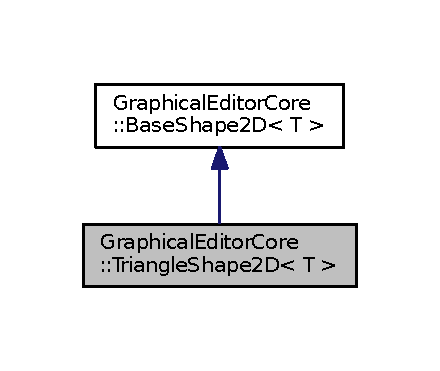
\includegraphics[width=211pt]{classGraphicalEditorCore_1_1TriangleShape2D__inherit__graph}
\end{center}
\end{figure}


Collaboration diagram for Graphical\+Editor\+Core\+:\+:Triangle\+Shape2D$<$ T $>$\+:
\nopagebreak
\begin{figure}[H]
\begin{center}
\leavevmode
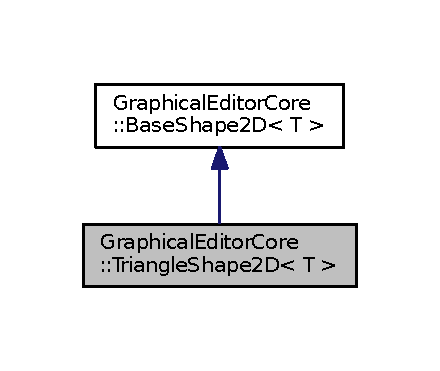
\includegraphics[width=211pt]{classGraphicalEditorCore_1_1TriangleShape2D__coll__graph}
\end{center}
\end{figure}
\subsection*{Public Member Functions}
\begin{DoxyCompactItemize}
\item 
\hyperlink{classGraphicalEditorCore_1_1TriangleShape2D_af0339a667c63abd464603bf68e8d4770}{Triangle\+Shape2D} (const size\+\_\+t \hyperlink{classGraphicalEditorCore_1_1BaseShape2D_ac66cfa23289ae36d70ff6b7c41dd791f}{id})
\item 
virtual \hyperlink{classGraphicalEditorCore_1_1TriangleShape2D_a561fbaff5077e2d945eb8a9a95c48617}{$\sim$\+Triangle\+Shape2D} ()
\item 
virtual void \hyperlink{classGraphicalEditorCore_1_1TriangleShape2D_a70baf8d77cdaa6107cac5ba2c8f9bc5b}{rotate} (const T clockwise\+\_\+angle) override
\item 
virtual void \hyperlink{classGraphicalEditorCore_1_1TriangleShape2D_a2b84784e80b932ef32641e7ac7d41bee}{move\+Center} (const T dx, const T dy) override
\item 
virtual void \hyperlink{classGraphicalEditorCore_1_1TriangleShape2D_a904d1d62d033013b636062c38df68d29}{move\+Vertex} (const T dx, const T dy, const size\+\_\+t index) override
\item 
virtual void \hyperlink{classGraphicalEditorCore_1_1TriangleShape2D_a769d7053c7410e288abeaa8e6122ee26}{scale} (const T factor) override
\end{DoxyCompactItemize}


\subsection{Constructor \& Destructor Documentation}
\index{Graphical\+Editor\+Core\+::\+Triangle\+Shape2D@{Graphical\+Editor\+Core\+::\+Triangle\+Shape2D}!Triangle\+Shape2D@{Triangle\+Shape2D}}
\index{Triangle\+Shape2D@{Triangle\+Shape2D}!Graphical\+Editor\+Core\+::\+Triangle\+Shape2D@{Graphical\+Editor\+Core\+::\+Triangle\+Shape2D}}
\subsubsection[{\texorpdfstring{Triangle\+Shape2\+D(const size\+\_\+t id)}{TriangleShape2D(const size_t id)}}]{\setlength{\rightskip}{0pt plus 5cm}template$<$typename T $>$ {\bf Graphical\+Editor\+Core\+::\+Triangle\+Shape2D}$<$ T $>$\+::{\bf Triangle\+Shape2D} (
\begin{DoxyParamCaption}
\item[{const size\+\_\+t}]{id}
\end{DoxyParamCaption}
)}\hypertarget{classGraphicalEditorCore_1_1TriangleShape2D_af0339a667c63abd464603bf68e8d4770}{}\label{classGraphicalEditorCore_1_1TriangleShape2D_af0339a667c63abd464603bf68e8d4770}
\index{Graphical\+Editor\+Core\+::\+Triangle\+Shape2D@{Graphical\+Editor\+Core\+::\+Triangle\+Shape2D}!````~Triangle\+Shape2D@{$\sim$\+Triangle\+Shape2D}}
\index{````~Triangle\+Shape2D@{$\sim$\+Triangle\+Shape2D}!Graphical\+Editor\+Core\+::\+Triangle\+Shape2D@{Graphical\+Editor\+Core\+::\+Triangle\+Shape2D}}
\subsubsection[{\texorpdfstring{$\sim$\+Triangle\+Shape2\+D()}{~TriangleShape2D()}}]{\setlength{\rightskip}{0pt plus 5cm}template$<$typename T $>$ {\bf Graphical\+Editor\+Core\+::\+Triangle\+Shape2D}$<$ T $>$\+::$\sim${\bf Triangle\+Shape2D} (
\begin{DoxyParamCaption}
{}
\end{DoxyParamCaption}
)\hspace{0.3cm}{\ttfamily [virtual]}}\hypertarget{classGraphicalEditorCore_1_1TriangleShape2D_a561fbaff5077e2d945eb8a9a95c48617}{}\label{classGraphicalEditorCore_1_1TriangleShape2D_a561fbaff5077e2d945eb8a9a95c48617}


\subsection{Member Function Documentation}
\index{Graphical\+Editor\+Core\+::\+Triangle\+Shape2D@{Graphical\+Editor\+Core\+::\+Triangle\+Shape2D}!move\+Center@{move\+Center}}
\index{move\+Center@{move\+Center}!Graphical\+Editor\+Core\+::\+Triangle\+Shape2D@{Graphical\+Editor\+Core\+::\+Triangle\+Shape2D}}
\subsubsection[{\texorpdfstring{move\+Center(const T dx, const T dy) override}{moveCenter(const T dx, const T dy) override}}]{\setlength{\rightskip}{0pt plus 5cm}template$<$typename T $>$ void {\bf Graphical\+Editor\+Core\+::\+Triangle\+Shape2D}$<$ T $>$\+::move\+Center (
\begin{DoxyParamCaption}
\item[{const T}]{dx, }
\item[{const T}]{dy}
\end{DoxyParamCaption}
)\hspace{0.3cm}{\ttfamily [override]}, {\ttfamily [virtual]}}\hypertarget{classGraphicalEditorCore_1_1TriangleShape2D_a2b84784e80b932ef32641e7ac7d41bee}{}\label{classGraphicalEditorCore_1_1TriangleShape2D_a2b84784e80b932ef32641e7ac7d41bee}


Implements \hyperlink{classGraphicalEditorCore_1_1BaseShape2D_adebef5c637da2c34a2fe728022740f94}{Graphical\+Editor\+Core\+::\+Base\+Shape2\+D$<$ T $>$}.

\index{Graphical\+Editor\+Core\+::\+Triangle\+Shape2D@{Graphical\+Editor\+Core\+::\+Triangle\+Shape2D}!move\+Vertex@{move\+Vertex}}
\index{move\+Vertex@{move\+Vertex}!Graphical\+Editor\+Core\+::\+Triangle\+Shape2D@{Graphical\+Editor\+Core\+::\+Triangle\+Shape2D}}
\subsubsection[{\texorpdfstring{move\+Vertex(const T dx, const T dy, const size\+\_\+t index) override}{moveVertex(const T dx, const T dy, const size_t index) override}}]{\setlength{\rightskip}{0pt plus 5cm}template$<$typename T $>$ void {\bf Graphical\+Editor\+Core\+::\+Triangle\+Shape2D}$<$ T $>$\+::move\+Vertex (
\begin{DoxyParamCaption}
\item[{const T}]{dx, }
\item[{const T}]{dy, }
\item[{const size\+\_\+t}]{index}
\end{DoxyParamCaption}
)\hspace{0.3cm}{\ttfamily [override]}, {\ttfamily [virtual]}}\hypertarget{classGraphicalEditorCore_1_1TriangleShape2D_a904d1d62d033013b636062c38df68d29}{}\label{classGraphicalEditorCore_1_1TriangleShape2D_a904d1d62d033013b636062c38df68d29}


Implements \hyperlink{classGraphicalEditorCore_1_1BaseShape2D_a9e6394ecf62e475a1d087e89258d4131}{Graphical\+Editor\+Core\+::\+Base\+Shape2\+D$<$ T $>$}.

\index{Graphical\+Editor\+Core\+::\+Triangle\+Shape2D@{Graphical\+Editor\+Core\+::\+Triangle\+Shape2D}!rotate@{rotate}}
\index{rotate@{rotate}!Graphical\+Editor\+Core\+::\+Triangle\+Shape2D@{Graphical\+Editor\+Core\+::\+Triangle\+Shape2D}}
\subsubsection[{\texorpdfstring{rotate(const T clockwise\+\_\+angle) override}{rotate(const T clockwise_angle) override}}]{\setlength{\rightskip}{0pt plus 5cm}template$<$typename T $>$ void {\bf Graphical\+Editor\+Core\+::\+Triangle\+Shape2D}$<$ T $>$\+::rotate (
\begin{DoxyParamCaption}
\item[{const T}]{clockwise\+\_\+angle}
\end{DoxyParamCaption}
)\hspace{0.3cm}{\ttfamily [override]}, {\ttfamily [virtual]}}\hypertarget{classGraphicalEditorCore_1_1TriangleShape2D_a70baf8d77cdaa6107cac5ba2c8f9bc5b}{}\label{classGraphicalEditorCore_1_1TriangleShape2D_a70baf8d77cdaa6107cac5ba2c8f9bc5b}


Implements \hyperlink{classGraphicalEditorCore_1_1BaseShape2D_a94a87b2fd8485cfb7d4ca97050d1bdde}{Graphical\+Editor\+Core\+::\+Base\+Shape2\+D$<$ T $>$}.

\index{Graphical\+Editor\+Core\+::\+Triangle\+Shape2D@{Graphical\+Editor\+Core\+::\+Triangle\+Shape2D}!scale@{scale}}
\index{scale@{scale}!Graphical\+Editor\+Core\+::\+Triangle\+Shape2D@{Graphical\+Editor\+Core\+::\+Triangle\+Shape2D}}
\subsubsection[{\texorpdfstring{scale(const T factor) override}{scale(const T factor) override}}]{\setlength{\rightskip}{0pt plus 5cm}template$<$typename T $>$ void {\bf Graphical\+Editor\+Core\+::\+Triangle\+Shape2D}$<$ T $>$\+::scale (
\begin{DoxyParamCaption}
\item[{const T}]{factor}
\end{DoxyParamCaption}
)\hspace{0.3cm}{\ttfamily [override]}, {\ttfamily [virtual]}}\hypertarget{classGraphicalEditorCore_1_1TriangleShape2D_a769d7053c7410e288abeaa8e6122ee26}{}\label{classGraphicalEditorCore_1_1TriangleShape2D_a769d7053c7410e288abeaa8e6122ee26}


Implements \hyperlink{classGraphicalEditorCore_1_1BaseShape2D_a2ff960ec57b180222a084642fa7dc780}{Graphical\+Editor\+Core\+::\+Base\+Shape2\+D$<$ T $>$}.



The documentation for this class was generated from the following files\+:\begin{DoxyCompactItemize}
\item 
05\+\_\+editor/\hyperlink{shapes__2d_8h}{shapes\+\_\+2d.\+h}\item 
05\+\_\+editor/\hyperlink{triangle__shape__2d_8cpp}{triangle\+\_\+shape\+\_\+2d.\+cpp}\end{DoxyCompactItemize}

\hypertarget{structtupple__printer}{}\section{tupple\+\_\+printer$<$ Tuple, n $>$ Struct Template Reference}
\label{structtupple__printer}\index{tupple\+\_\+printer$<$ Tuple, n $>$@{tupple\+\_\+printer$<$ Tuple, n $>$}}


{\ttfamily \#include $<$print\+\_\+ip\+\_\+04.\+hpp$>$}

\subsection*{Static Public Member Functions}
\begin{DoxyCompactItemize}
\item 
static void \hyperlink{structtupple__printer_a85dd6fb2430ea3eaff7f58558adcefb9}{print} (const Tuple \&t, const std\+::string \&delimeter\+\_\+str=\char`\"{}, \char`\"{})
\end{DoxyCompactItemize}


\subsection{Detailed Description}
\subsubsection*{template$<$class Tuple, size\+\_\+t n$>$\\*
struct tupple\+\_\+printer$<$ Tuple, n $>$}

Prints tuple of any size. 

\subsection{Member Function Documentation}
\index{tupple\+\_\+printer@{tupple\+\_\+printer}!print@{print}}
\index{print@{print}!tupple\+\_\+printer@{tupple\+\_\+printer}}
\subsubsection[{\texorpdfstring{print(const Tuple \&t, const std\+::string \&delimeter\+\_\+str="", "")}{print(const Tuple &t, const std::string &delimeter_str=", ")}}]{\setlength{\rightskip}{0pt plus 5cm}template$<$class Tuple, size\+\_\+t n$>$ static void {\bf tupple\+\_\+printer}$<$ Tuple, n $>$\+::print (
\begin{DoxyParamCaption}
\item[{const Tuple \&}]{t, }
\item[{const std\+::string \&}]{delimeter\+\_\+str = {\ttfamily \char`\"{},~\char`\"{}}}
\end{DoxyParamCaption}
)\hspace{0.3cm}{\ttfamily [inline]}, {\ttfamily [static]}}\hypertarget{structtupple__printer_a85dd6fb2430ea3eaff7f58558adcefb9}{}\label{structtupple__printer_a85dd6fb2430ea3eaff7f58558adcefb9}


The documentation for this struct was generated from the following file\+:\begin{DoxyCompactItemize}
\item 
04\+\_\+sfinae/\hyperlink{print__ip__04_8hpp}{print\+\_\+ip\+\_\+04.\+hpp}\end{DoxyCompactItemize}

\hypertarget{structtupple__printer_3_01Tuple_00_011_01_4}{}\section{tupple\+\_\+printer$<$ Tuple, 1 $>$ Struct Template Reference}
\label{structtupple__printer_3_01Tuple_00_011_01_4}\index{tupple\+\_\+printer$<$ Tuple, 1 $>$@{tupple\+\_\+printer$<$ Tuple, 1 $>$}}


{\ttfamily \#include $<$print\+\_\+ip\+\_\+04.\+hpp$>$}

\subsection*{Static Public Member Functions}
\begin{DoxyCompactItemize}
\item 
static void \hyperlink{structtupple__printer_3_01Tuple_00_011_01_4_aa1465f1c21683b29c615f5ea48a4d986}{print} (const Tuple \&t, const std\+::string \&)
\end{DoxyCompactItemize}


\subsection{Member Function Documentation}
\index{tupple\+\_\+printer$<$ Tuple, 1 $>$@{tupple\+\_\+printer$<$ Tuple, 1 $>$}!print@{print}}
\index{print@{print}!tupple\+\_\+printer$<$ Tuple, 1 $>$@{tupple\+\_\+printer$<$ Tuple, 1 $>$}}
\subsubsection[{\texorpdfstring{print(const Tuple \&t, const std\+::string \&)}{print(const Tuple &t, const std::string &)}}]{\setlength{\rightskip}{0pt plus 5cm}template$<$class Tuple $>$ static void {\bf tupple\+\_\+printer}$<$ Tuple, 1 $>$\+::print (
\begin{DoxyParamCaption}
\item[{const Tuple \&}]{t, }
\item[{const std\+::string \&}]{}
\end{DoxyParamCaption}
)\hspace{0.3cm}{\ttfamily [inline]}, {\ttfamily [static]}}\hypertarget{structtupple__printer_3_01Tuple_00_011_01_4_aa1465f1c21683b29c615f5ea48a4d986}{}\label{structtupple__printer_3_01Tuple_00_011_01_4_aa1465f1c21683b29c615f5ea48a4d986}


The documentation for this struct was generated from the following file\+:\begin{DoxyCompactItemize}
\item 
04\+\_\+sfinae/\hyperlink{print__ip__04_8hpp}{print\+\_\+ip\+\_\+04.\+hpp}\end{DoxyCompactItemize}

\chapter{File Documentation}
\hypertarget{01_2main_8cpp}{}\section{01/main.cpp File Reference}
\label{01_2main_8cpp}\index{01/main.\+cpp@{01/main.\+cpp}}
{\ttfamily \#include $<$iostream$>$}\\*
{\ttfamily \#include \char`\"{}vers\+\_\+lib.\+h\char`\"{}}\\*
Include dependency graph for main.\+cpp\+:
\nopagebreak
\begin{figure}[H]
\begin{center}
\leavevmode
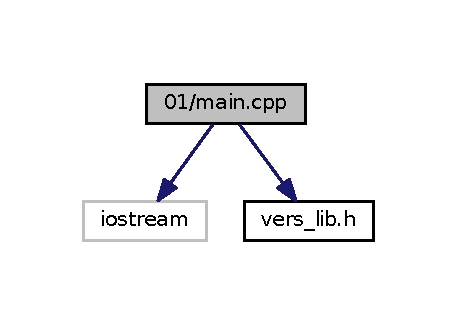
\includegraphics[width=220pt]{01_2main_8cpp__incl}
\end{center}
\end{figure}
\subsection*{Functions}
\begin{DoxyCompactItemize}
\item 
int \hyperlink{01_2main_8cpp_ae66f6b31b5ad750f1fe042a706a4e3d4}{main} ()
\end{DoxyCompactItemize}


\subsection{Function Documentation}
\index{01/main.\+cpp@{01/main.\+cpp}!main@{main}}
\index{main@{main}!01/main.\+cpp@{01/main.\+cpp}}
\subsubsection[{\texorpdfstring{main()}{main()}}]{\setlength{\rightskip}{0pt plus 5cm}int main (
\begin{DoxyParamCaption}
{}
\end{DoxyParamCaption}
)}\hypertarget{01_2main_8cpp_ae66f6b31b5ad750f1fe042a706a4e3d4}{}\label{01_2main_8cpp_ae66f6b31b5ad750f1fe042a706a4e3d4}

\hypertarget{04__sfinae_2main_8cpp}{}\section{04\+\_\+sfinae/main.cpp File Reference}
\label{04__sfinae_2main_8cpp}\index{04\+\_\+sfinae/main.\+cpp@{04\+\_\+sfinae/main.\+cpp}}
{\ttfamily \#include $<$iostream$>$}\\*
{\ttfamily \#include $<$string$>$}\\*
{\ttfamily \#include $<$map$>$}\\*
{\ttfamily \#include \char`\"{}print\+\_\+ip\+\_\+04.\+hpp\char`\"{}}\\*
Include dependency graph for main.\+cpp\+:
\nopagebreak
\begin{figure}[H]
\begin{center}
\leavevmode
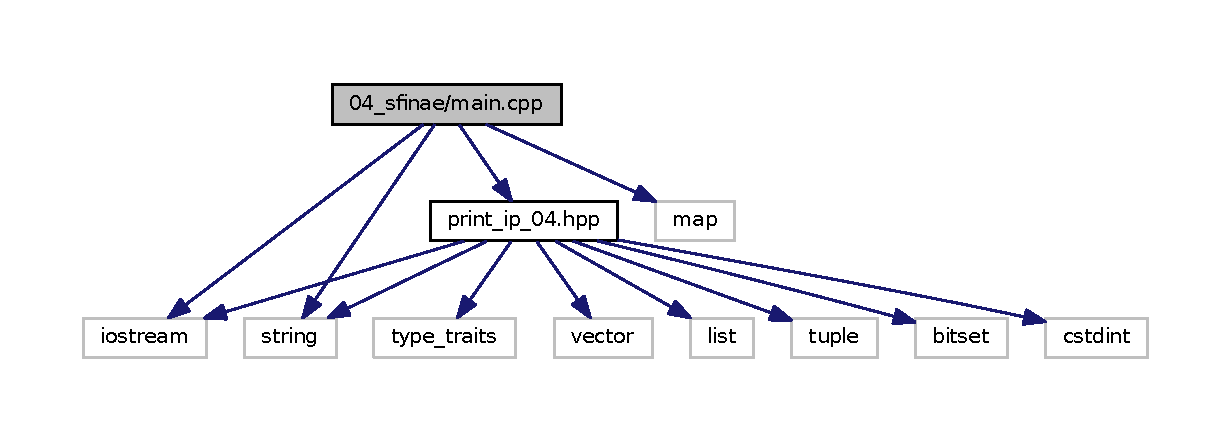
\includegraphics[width=350pt]{04__sfinae_2main_8cpp__incl}
\end{center}
\end{figure}
\subsection*{Functions}
\begin{DoxyCompactItemize}
\item 
int \hyperlink{04__sfinae_2main_8cpp_a0ddf1224851353fc92bfbff6f499fa97}{main} (int argc, char $\ast$argv\mbox{[}$\,$\mbox{]})
\end{DoxyCompactItemize}


\subsection{Function Documentation}
\index{04\+\_\+sfinae/main.\+cpp@{04\+\_\+sfinae/main.\+cpp}!main@{main}}
\index{main@{main}!04\+\_\+sfinae/main.\+cpp@{04\+\_\+sfinae/main.\+cpp}}
\subsubsection[{\texorpdfstring{main(int argc, char $\ast$argv[])}{main(int argc, char *argv[])}}]{\setlength{\rightskip}{0pt plus 5cm}int main (
\begin{DoxyParamCaption}
\item[{int}]{argc, }
\item[{char $\ast$}]{argv\mbox{[}$\,$\mbox{]}}
\end{DoxyParamCaption}
)}\hypertarget{04__sfinae_2main_8cpp_a0ddf1224851353fc92bfbff6f499fa97}{}\label{04__sfinae_2main_8cpp_a0ddf1224851353fc92bfbff6f499fa97}

\hypertarget{05__editor_2main_8cpp}{}\section{05\+\_\+editor/main.cpp File Reference}
\label{05__editor_2main_8cpp}\index{05\+\_\+editor/main.\+cpp@{05\+\_\+editor/main.\+cpp}}
{\ttfamily \#include \char`\"{}editor\+\_\+core.\+h\char`\"{}}\\*
{\ttfamily \#include $<$memory$>$}\\*
Include dependency graph for main.\+cpp\+:
\nopagebreak
\begin{figure}[H]
\begin{center}
\leavevmode
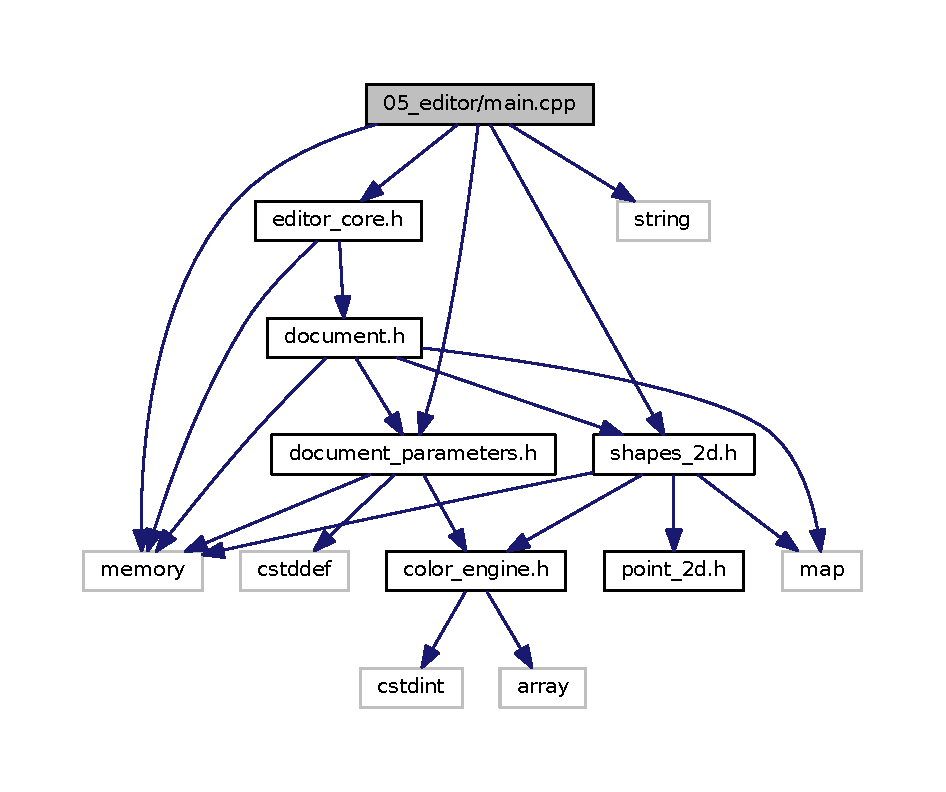
\includegraphics[width=236pt]{05__editor_2main_8cpp__incl}
\end{center}
\end{figure}
\subsection*{Functions}
\begin{DoxyCompactItemize}
\item 
int \hyperlink{05__editor_2main_8cpp_a0ddf1224851353fc92bfbff6f499fa97}{main} (int argc, char $\ast$argv\mbox{[}$\,$\mbox{]})
\end{DoxyCompactItemize}


\subsection{Function Documentation}
\index{05\+\_\+editor/main.\+cpp@{05\+\_\+editor/main.\+cpp}!main@{main}}
\index{main@{main}!05\+\_\+editor/main.\+cpp@{05\+\_\+editor/main.\+cpp}}
\subsubsection[{\texorpdfstring{main(int argc, char $\ast$argv[])}{main(int argc, char *argv[])}}]{\setlength{\rightskip}{0pt plus 5cm}int main (
\begin{DoxyParamCaption}
\item[{int}]{argc, }
\item[{char $\ast$}]{argv\mbox{[}$\,$\mbox{]}}
\end{DoxyParamCaption}
)}\hypertarget{05__editor_2main_8cpp_a0ddf1224851353fc92bfbff6f499fa97}{}\label{05__editor_2main_8cpp_a0ddf1224851353fc92bfbff6f499fa97}

\hypertarget{06__matrix_2main_8cpp}{}\section{06\+\_\+matrix/main.cpp File Reference}
\label{06__matrix_2main_8cpp}\index{06\+\_\+matrix/main.\+cpp@{06\+\_\+matrix/main.\+cpp}}
{\ttfamily \#include $<$iostream$>$}\\*
Include dependency graph for main.\+cpp\+:
\nopagebreak
\begin{figure}[H]
\begin{center}
\leavevmode
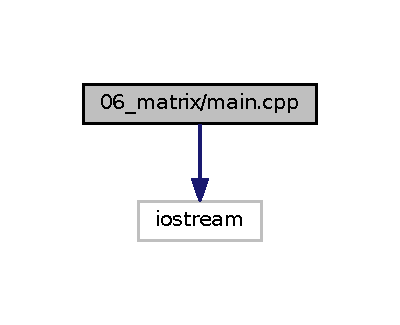
\includegraphics[width=192pt]{06__matrix_2main_8cpp__incl}
\end{center}
\end{figure}
\subsection*{Functions}
\begin{DoxyCompactItemize}
\item 
int \hyperlink{06__matrix_2main_8cpp_a0ddf1224851353fc92bfbff6f499fa97}{main} (int argc, char $\ast$argv\mbox{[}$\,$\mbox{]})
\end{DoxyCompactItemize}


\subsection{Function Documentation}
\index{06\+\_\+matrix/main.\+cpp@{06\+\_\+matrix/main.\+cpp}!main@{main}}
\index{main@{main}!06\+\_\+matrix/main.\+cpp@{06\+\_\+matrix/main.\+cpp}}
\subsubsection[{\texorpdfstring{main(int argc, char $\ast$argv[])}{main(int argc, char *argv[])}}]{\setlength{\rightskip}{0pt plus 5cm}int main (
\begin{DoxyParamCaption}
\item[{int}]{argc, }
\item[{char $\ast$}]{argv\mbox{[}$\,$\mbox{]}}
\end{DoxyParamCaption}
)}\hypertarget{06__matrix_2main_8cpp_a0ddf1224851353fc92bfbff6f499fa97}{}\label{06__matrix_2main_8cpp_a0ddf1224851353fc92bfbff6f499fa97}

\hypertarget{multithread__pc_2main_8cpp}{}\section{multithread\+\_\+pc/main.cpp File Reference}
\label{multithread__pc_2main_8cpp}\index{multithread\+\_\+pc/main.\+cpp@{multithread\+\_\+pc/main.\+cpp}}
{\ttfamily \#include \char`\"{}prod\+\_\+cons\+\_\+simulator.\+h\char`\"{}}\\*
{\ttfamily \#include $<$memory$>$}\\*
{\ttfamily \#include $<$iostream$>$}\\*
Include dependency graph for main.\+cpp\+:
\nopagebreak
\begin{figure}[H]
\begin{center}
\leavevmode
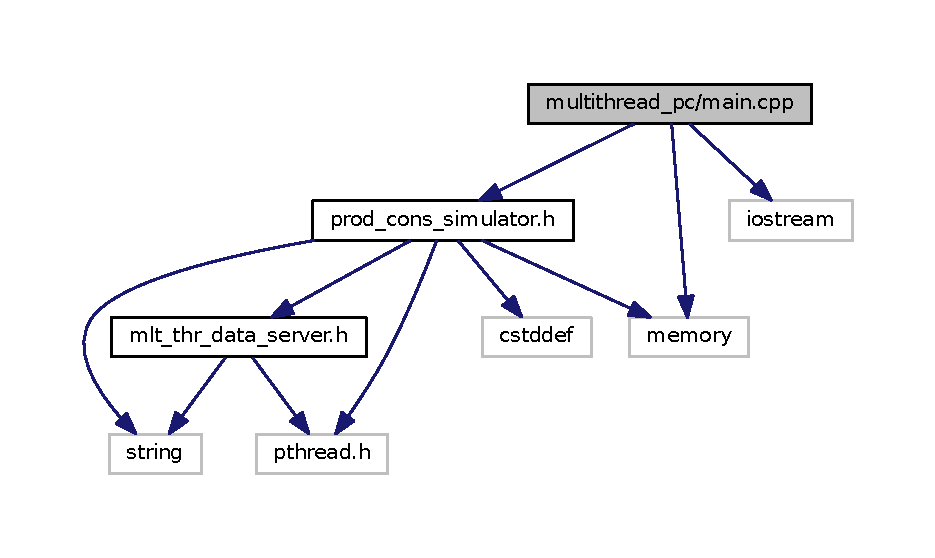
\includegraphics[width=350pt]{multithread__pc_2main_8cpp__incl}
\end{center}
\end{figure}
\subsection*{Functions}
\begin{DoxyCompactItemize}
\item 
void \hyperlink{multithread__pc_2main_8cpp_a853216ac51aa181669ff4d3de74058a7}{print\+\_\+help} ()
\item 
int \hyperlink{multithread__pc_2main_8cpp_a0ddf1224851353fc92bfbff6f499fa97}{main} (int argc, char $\ast$argv\mbox{[}$\,$\mbox{]})
\end{DoxyCompactItemize}


\subsection{Function Documentation}
\index{multithread\+\_\+pc/main.\+cpp@{multithread\+\_\+pc/main.\+cpp}!main@{main}}
\index{main@{main}!multithread\+\_\+pc/main.\+cpp@{multithread\+\_\+pc/main.\+cpp}}
\subsubsection[{\texorpdfstring{main(int argc, char $\ast$argv[])}{main(int argc, char *argv[])}}]{\setlength{\rightskip}{0pt plus 5cm}int main (
\begin{DoxyParamCaption}
\item[{int}]{argc, }
\item[{char $\ast$}]{argv\mbox{[}$\,$\mbox{]}}
\end{DoxyParamCaption}
)}\hypertarget{multithread__pc_2main_8cpp_a0ddf1224851353fc92bfbff6f499fa97}{}\label{multithread__pc_2main_8cpp_a0ddf1224851353fc92bfbff6f499fa97}
\index{multithread\+\_\+pc/main.\+cpp@{multithread\+\_\+pc/main.\+cpp}!print\+\_\+help@{print\+\_\+help}}
\index{print\+\_\+help@{print\+\_\+help}!multithread\+\_\+pc/main.\+cpp@{multithread\+\_\+pc/main.\+cpp}}
\subsubsection[{\texorpdfstring{print\+\_\+help()}{print_help()}}]{\setlength{\rightskip}{0pt plus 5cm}void print\+\_\+help (
\begin{DoxyParamCaption}
{}
\end{DoxyParamCaption}
)}\hypertarget{multithread__pc_2main_8cpp_a853216ac51aa181669ff4d3de74058a7}{}\label{multithread__pc_2main_8cpp_a853216ac51aa181669ff4d3de74058a7}

\hypertarget{test__vers__boost_8cpp}{}\section{01/test\+\_\+vers\+\_\+boost.cpp File Reference}
\label{test__vers__boost_8cpp}\index{01/test\+\_\+vers\+\_\+boost.\+cpp@{01/test\+\_\+vers\+\_\+boost.\+cpp}}
{\ttfamily \#include $<$boost/test/unit\+\_\+test.\+hpp$>$}\\*
{\ttfamily \#include \char`\"{}vers\+\_\+lib.\+h\char`\"{}}\\*
Include dependency graph for test\+\_\+vers\+\_\+boost.\+cpp\+:
\nopagebreak
\begin{figure}[H]
\begin{center}
\leavevmode
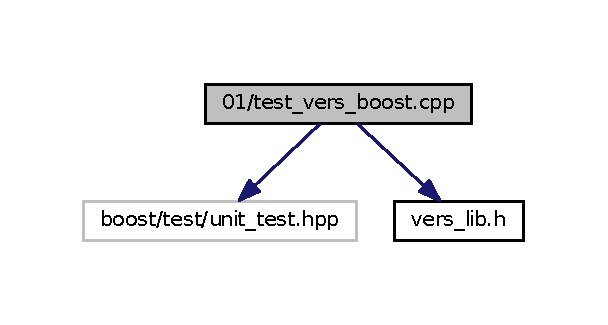
\includegraphics[width=292pt]{test__vers__boost_8cpp__incl}
\end{center}
\end{figure}
\subsection*{Macros}
\begin{DoxyCompactItemize}
\item 
\#define \hyperlink{test__vers__boost_8cpp_a6b2a3852db8bb19ab6909bac01859985}{B\+O\+O\+S\+T\+\_\+\+T\+E\+S\+T\+\_\+\+M\+O\+D\+U\+LE}~test\+\_\+vers\+\_\+boost
\end{DoxyCompactItemize}
\subsection*{Functions}
\begin{DoxyCompactItemize}
\item 
\hyperlink{test__vers__boost_8cpp_a5a8f1e117b104260d857ed534915b417}{B\+O\+O\+S\+T\+\_\+\+A\+U\+T\+O\+\_\+\+T\+E\+S\+T\+\_\+\+C\+A\+SE} (test\+\_\+valid\+\_\+version)
\end{DoxyCompactItemize}


\subsection{Macro Definition Documentation}
\index{test\+\_\+vers\+\_\+boost.\+cpp@{test\+\_\+vers\+\_\+boost.\+cpp}!B\+O\+O\+S\+T\+\_\+\+T\+E\+S\+T\+\_\+\+M\+O\+D\+U\+LE@{B\+O\+O\+S\+T\+\_\+\+T\+E\+S\+T\+\_\+\+M\+O\+D\+U\+LE}}
\index{B\+O\+O\+S\+T\+\_\+\+T\+E\+S\+T\+\_\+\+M\+O\+D\+U\+LE@{B\+O\+O\+S\+T\+\_\+\+T\+E\+S\+T\+\_\+\+M\+O\+D\+U\+LE}!test\+\_\+vers\+\_\+boost.\+cpp@{test\+\_\+vers\+\_\+boost.\+cpp}}
\subsubsection[{\texorpdfstring{B\+O\+O\+S\+T\+\_\+\+T\+E\+S\+T\+\_\+\+M\+O\+D\+U\+LE}{BOOST_TEST_MODULE}}]{\setlength{\rightskip}{0pt plus 5cm}\#define B\+O\+O\+S\+T\+\_\+\+T\+E\+S\+T\+\_\+\+M\+O\+D\+U\+LE~test\+\_\+vers\+\_\+boost}\hypertarget{test__vers__boost_8cpp_a6b2a3852db8bb19ab6909bac01859985}{}\label{test__vers__boost_8cpp_a6b2a3852db8bb19ab6909bac01859985}


\subsection{Function Documentation}
\index{test\+\_\+vers\+\_\+boost.\+cpp@{test\+\_\+vers\+\_\+boost.\+cpp}!B\+O\+O\+S\+T\+\_\+\+A\+U\+T\+O\+\_\+\+T\+E\+S\+T\+\_\+\+C\+A\+SE@{B\+O\+O\+S\+T\+\_\+\+A\+U\+T\+O\+\_\+\+T\+E\+S\+T\+\_\+\+C\+A\+SE}}
\index{B\+O\+O\+S\+T\+\_\+\+A\+U\+T\+O\+\_\+\+T\+E\+S\+T\+\_\+\+C\+A\+SE@{B\+O\+O\+S\+T\+\_\+\+A\+U\+T\+O\+\_\+\+T\+E\+S\+T\+\_\+\+C\+A\+SE}!test\+\_\+vers\+\_\+boost.\+cpp@{test\+\_\+vers\+\_\+boost.\+cpp}}
\subsubsection[{\texorpdfstring{B\+O\+O\+S\+T\+\_\+\+A\+U\+T\+O\+\_\+\+T\+E\+S\+T\+\_\+\+C\+A\+S\+E(test\+\_\+valid\+\_\+version)}{BOOST_AUTO_TEST_CASE(test_valid_version)}}]{\setlength{\rightskip}{0pt plus 5cm}B\+O\+O\+S\+T\+\_\+\+A\+U\+T\+O\+\_\+\+T\+E\+S\+T\+\_\+\+C\+A\+SE (
\begin{DoxyParamCaption}
\item[{test\+\_\+valid\+\_\+version}]{}
\end{DoxyParamCaption}
)}\hypertarget{test__vers__boost_8cpp_a5a8f1e117b104260d857ed534915b417}{}\label{test__vers__boost_8cpp_a5a8f1e117b104260d857ed534915b417}

\hypertarget{test__vers__gtest_8cpp}{}\section{01/test\+\_\+vers\+\_\+gtest.cpp File Reference}
\label{test__vers__gtest_8cpp}\index{01/test\+\_\+vers\+\_\+gtest.\+cpp@{01/test\+\_\+vers\+\_\+gtest.\+cpp}}
{\ttfamily \#include $<$gtest/gtest.\+h$>$}\\*
{\ttfamily \#include \char`\"{}vers\+\_\+lib.\+h\char`\"{}}\\*
Include dependency graph for test\+\_\+vers\+\_\+gtest.\+cpp\+:
\nopagebreak
\begin{figure}[H]
\begin{center}
\leavevmode
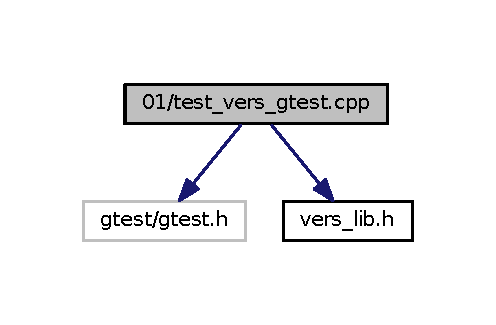
\includegraphics[width=238pt]{test__vers__gtest_8cpp__incl}
\end{center}
\end{figure}
\subsection*{Functions}
\begin{DoxyCompactItemize}
\item 
\hyperlink{test__vers__gtest_8cpp_ad040b370b89121e8a68bf66636367f02}{T\+E\+ST} (test\+\_\+vers\+\_\+gtest, valid\+\_\+versions)
\item 
int \hyperlink{test__vers__gtest_8cpp_a0ddf1224851353fc92bfbff6f499fa97}{main} (int argc, char $\ast$argv\mbox{[}$\,$\mbox{]})
\end{DoxyCompactItemize}


\subsection{Function Documentation}
\index{test\+\_\+vers\+\_\+gtest.\+cpp@{test\+\_\+vers\+\_\+gtest.\+cpp}!main@{main}}
\index{main@{main}!test\+\_\+vers\+\_\+gtest.\+cpp@{test\+\_\+vers\+\_\+gtest.\+cpp}}
\subsubsection[{\texorpdfstring{main(int argc, char $\ast$argv[])}{main(int argc, char *argv[])}}]{\setlength{\rightskip}{0pt plus 5cm}int main (
\begin{DoxyParamCaption}
\item[{int}]{argc, }
\item[{char $\ast$}]{argv\mbox{[}$\,$\mbox{]}}
\end{DoxyParamCaption}
)}\hypertarget{test__vers__gtest_8cpp_a0ddf1224851353fc92bfbff6f499fa97}{}\label{test__vers__gtest_8cpp_a0ddf1224851353fc92bfbff6f499fa97}
\index{test\+\_\+vers\+\_\+gtest.\+cpp@{test\+\_\+vers\+\_\+gtest.\+cpp}!T\+E\+ST@{T\+E\+ST}}
\index{T\+E\+ST@{T\+E\+ST}!test\+\_\+vers\+\_\+gtest.\+cpp@{test\+\_\+vers\+\_\+gtest.\+cpp}}
\subsubsection[{\texorpdfstring{T\+E\+S\+T(test\+\_\+vers\+\_\+gtest, valid\+\_\+versions)}{TEST(test_vers_gtest, valid_versions)}}]{\setlength{\rightskip}{0pt plus 5cm}T\+E\+ST (
\begin{DoxyParamCaption}
\item[{test\+\_\+vers\+\_\+gtest}]{, }
\item[{valid\+\_\+versions}]{}
\end{DoxyParamCaption}
)}\hypertarget{test__vers__gtest_8cpp_ad040b370b89121e8a68bf66636367f02}{}\label{test__vers__gtest_8cpp_ad040b370b89121e8a68bf66636367f02}

\hypertarget{vers__lib_8cpp}{}\section{01/vers\+\_\+lib.cpp File Reference}
\label{vers__lib_8cpp}\index{01/vers\+\_\+lib.\+cpp@{01/vers\+\_\+lib.\+cpp}}
{\ttfamily \#include \char`\"{}vers\+\_\+lib.\+h\char`\"{}}\\*
{\ttfamily \#include \char`\"{}version.\+h\char`\"{}}\\*
Include dependency graph for vers\+\_\+lib.\+cpp\+:
\nopagebreak
\begin{figure}[H]
\begin{center}
\leavevmode
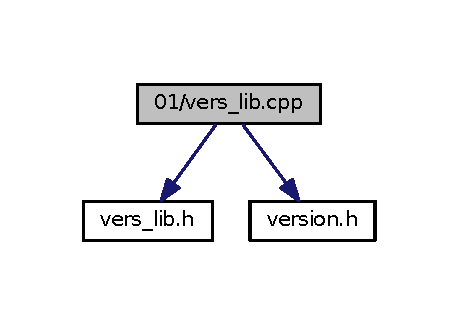
\includegraphics[width=220pt]{vers__lib_8cpp__incl}
\end{center}
\end{figure}
\subsection*{Functions}
\begin{DoxyCompactItemize}
\item 
int \hyperlink{vers__lib_8cpp_aa9387ddec2c78390f4fdf3b979348d62}{version\+\_\+major} () noexcept
\item 
int \hyperlink{vers__lib_8cpp_a5de5ba4c90576bf63ff2d44a821feb48}{version\+\_\+minor} () noexcept
\item 
int \hyperlink{vers__lib_8cpp_ac2c281eb9fc0ae960c904d8f7dfd082c}{version\+\_\+patch} () noexcept
\end{DoxyCompactItemize}


\subsection{Function Documentation}
\index{vers\+\_\+lib.\+cpp@{vers\+\_\+lib.\+cpp}!version\+\_\+major@{version\+\_\+major}}
\index{version\+\_\+major@{version\+\_\+major}!vers\+\_\+lib.\+cpp@{vers\+\_\+lib.\+cpp}}
\subsubsection[{\texorpdfstring{version\+\_\+major() noexcept}{version_major() noexcept}}]{\setlength{\rightskip}{0pt plus 5cm}int version\+\_\+major (
\begin{DoxyParamCaption}
{}
\end{DoxyParamCaption}
)\hspace{0.3cm}{\ttfamily [noexcept]}}\hypertarget{vers__lib_8cpp_aa9387ddec2c78390f4fdf3b979348d62}{}\label{vers__lib_8cpp_aa9387ddec2c78390f4fdf3b979348d62}
\index{vers\+\_\+lib.\+cpp@{vers\+\_\+lib.\+cpp}!version\+\_\+minor@{version\+\_\+minor}}
\index{version\+\_\+minor@{version\+\_\+minor}!vers\+\_\+lib.\+cpp@{vers\+\_\+lib.\+cpp}}
\subsubsection[{\texorpdfstring{version\+\_\+minor() noexcept}{version_minor() noexcept}}]{\setlength{\rightskip}{0pt plus 5cm}int version\+\_\+minor (
\begin{DoxyParamCaption}
{}
\end{DoxyParamCaption}
)\hspace{0.3cm}{\ttfamily [noexcept]}}\hypertarget{vers__lib_8cpp_a5de5ba4c90576bf63ff2d44a821feb48}{}\label{vers__lib_8cpp_a5de5ba4c90576bf63ff2d44a821feb48}
\index{vers\+\_\+lib.\+cpp@{vers\+\_\+lib.\+cpp}!version\+\_\+patch@{version\+\_\+patch}}
\index{version\+\_\+patch@{version\+\_\+patch}!vers\+\_\+lib.\+cpp@{vers\+\_\+lib.\+cpp}}
\subsubsection[{\texorpdfstring{version\+\_\+patch() noexcept}{version_patch() noexcept}}]{\setlength{\rightskip}{0pt plus 5cm}int version\+\_\+patch (
\begin{DoxyParamCaption}
{}
\end{DoxyParamCaption}
)\hspace{0.3cm}{\ttfamily [noexcept]}}\hypertarget{vers__lib_8cpp_ac2c281eb9fc0ae960c904d8f7dfd082c}{}\label{vers__lib_8cpp_ac2c281eb9fc0ae960c904d8f7dfd082c}

\hypertarget{vers__lib_8h}{}\section{01/vers\+\_\+lib.h File Reference}
\label{vers__lib_8h}\index{01/vers\+\_\+lib.\+h@{01/vers\+\_\+lib.\+h}}
This graph shows which files directly or indirectly include this file\+:
\nopagebreak
\begin{figure}[H]
\begin{center}
\leavevmode
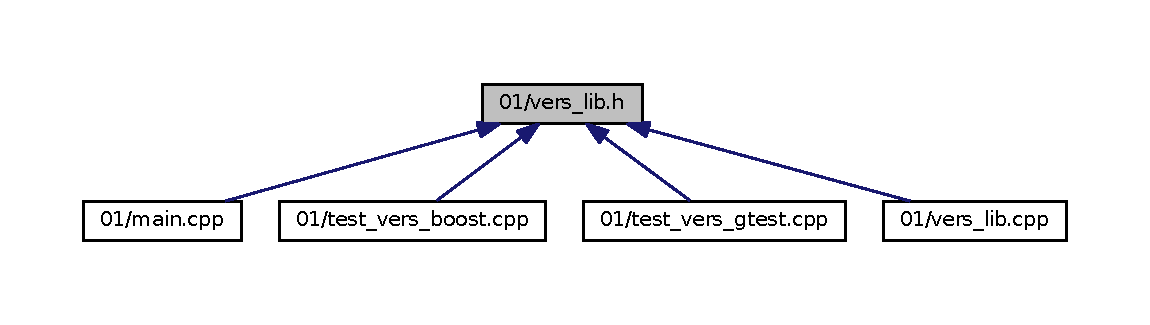
\includegraphics[width=350pt]{vers__lib_8h__dep__incl}
\end{center}
\end{figure}
\subsection*{Functions}
\begin{DoxyCompactItemize}
\item 
int \hyperlink{vers__lib_8h_aa9387ddec2c78390f4fdf3b979348d62}{version\+\_\+major} () noexcept
\item 
int \hyperlink{vers__lib_8h_a5de5ba4c90576bf63ff2d44a821feb48}{version\+\_\+minor} () noexcept
\item 
int \hyperlink{vers__lib_8h_ac2c281eb9fc0ae960c904d8f7dfd082c}{version\+\_\+patch} () noexcept
\end{DoxyCompactItemize}


\subsection{Function Documentation}
\index{vers\+\_\+lib.\+h@{vers\+\_\+lib.\+h}!version\+\_\+major@{version\+\_\+major}}
\index{version\+\_\+major@{version\+\_\+major}!vers\+\_\+lib.\+h@{vers\+\_\+lib.\+h}}
\subsubsection[{\texorpdfstring{version\+\_\+major() noexcept}{version_major() noexcept}}]{\setlength{\rightskip}{0pt plus 5cm}int version\+\_\+major (
\begin{DoxyParamCaption}
{}
\end{DoxyParamCaption}
)\hspace{0.3cm}{\ttfamily [noexcept]}}\hypertarget{vers__lib_8h_aa9387ddec2c78390f4fdf3b979348d62}{}\label{vers__lib_8h_aa9387ddec2c78390f4fdf3b979348d62}
\index{vers\+\_\+lib.\+h@{vers\+\_\+lib.\+h}!version\+\_\+minor@{version\+\_\+minor}}
\index{version\+\_\+minor@{version\+\_\+minor}!vers\+\_\+lib.\+h@{vers\+\_\+lib.\+h}}
\subsubsection[{\texorpdfstring{version\+\_\+minor() noexcept}{version_minor() noexcept}}]{\setlength{\rightskip}{0pt plus 5cm}int version\+\_\+minor (
\begin{DoxyParamCaption}
{}
\end{DoxyParamCaption}
)\hspace{0.3cm}{\ttfamily [noexcept]}}\hypertarget{vers__lib_8h_a5de5ba4c90576bf63ff2d44a821feb48}{}\label{vers__lib_8h_a5de5ba4c90576bf63ff2d44a821feb48}
\index{vers\+\_\+lib.\+h@{vers\+\_\+lib.\+h}!version\+\_\+patch@{version\+\_\+patch}}
\index{version\+\_\+patch@{version\+\_\+patch}!vers\+\_\+lib.\+h@{vers\+\_\+lib.\+h}}
\subsubsection[{\texorpdfstring{version\+\_\+patch() noexcept}{version_patch() noexcept}}]{\setlength{\rightskip}{0pt plus 5cm}int version\+\_\+patch (
\begin{DoxyParamCaption}
{}
\end{DoxyParamCaption}
)\hspace{0.3cm}{\ttfamily [noexcept]}}\hypertarget{vers__lib_8h_ac2c281eb9fc0ae960c904d8f7dfd082c}{}\label{vers__lib_8h_ac2c281eb9fc0ae960c904d8f7dfd082c}

\hypertarget{version_8h}{}\section{01/version.h File Reference}
\label{version_8h}\index{01/version.\+h@{01/version.\+h}}
This graph shows which files directly or indirectly include this file\+:
\nopagebreak
\begin{figure}[H]
\begin{center}
\leavevmode
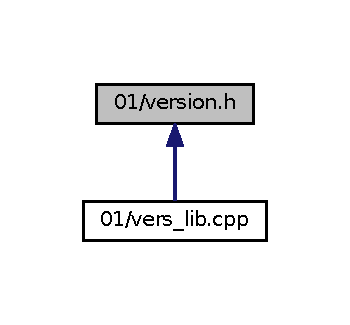
\includegraphics[width=168pt]{version_8h__dep__incl}
\end{center}
\end{figure}
\subsection*{Macros}
\begin{DoxyCompactItemize}
\item 
\#define \hyperlink{version_8h_a4a5fc96a4bdd7d68ed99ccce9ca2e77e}{P\+R\+O\+J\+E\+C\+T\+\_\+\+V\+E\+R\+S\+I\+O\+N\+\_\+\+P\+A\+T\+CH}~1
\item 
\#define \hyperlink{version_8h_a43e23009192a3e216fefec17750d8673}{P\+R\+O\+J\+E\+C\+T\+\_\+\+V\+E\+R\+S\+I\+O\+N\+\_\+\+M\+I\+N\+OR}~0
\item 
\#define \hyperlink{version_8h_abecd2198575b690d25a741857f8390d1}{P\+R\+O\+J\+E\+C\+T\+\_\+\+V\+E\+R\+S\+I\+O\+N\+\_\+\+M\+A\+J\+OR}~0
\end{DoxyCompactItemize}


\subsection{Macro Definition Documentation}
\index{version.\+h@{version.\+h}!P\+R\+O\+J\+E\+C\+T\+\_\+\+V\+E\+R\+S\+I\+O\+N\+\_\+\+M\+A\+J\+OR@{P\+R\+O\+J\+E\+C\+T\+\_\+\+V\+E\+R\+S\+I\+O\+N\+\_\+\+M\+A\+J\+OR}}
\index{P\+R\+O\+J\+E\+C\+T\+\_\+\+V\+E\+R\+S\+I\+O\+N\+\_\+\+M\+A\+J\+OR@{P\+R\+O\+J\+E\+C\+T\+\_\+\+V\+E\+R\+S\+I\+O\+N\+\_\+\+M\+A\+J\+OR}!version.\+h@{version.\+h}}
\subsubsection[{\texorpdfstring{P\+R\+O\+J\+E\+C\+T\+\_\+\+V\+E\+R\+S\+I\+O\+N\+\_\+\+M\+A\+J\+OR}{PROJECT_VERSION_MAJOR}}]{\setlength{\rightskip}{0pt plus 5cm}\#define P\+R\+O\+J\+E\+C\+T\+\_\+\+V\+E\+R\+S\+I\+O\+N\+\_\+\+M\+A\+J\+OR~0}\hypertarget{version_8h_abecd2198575b690d25a741857f8390d1}{}\label{version_8h_abecd2198575b690d25a741857f8390d1}
\index{version.\+h@{version.\+h}!P\+R\+O\+J\+E\+C\+T\+\_\+\+V\+E\+R\+S\+I\+O\+N\+\_\+\+M\+I\+N\+OR@{P\+R\+O\+J\+E\+C\+T\+\_\+\+V\+E\+R\+S\+I\+O\+N\+\_\+\+M\+I\+N\+OR}}
\index{P\+R\+O\+J\+E\+C\+T\+\_\+\+V\+E\+R\+S\+I\+O\+N\+\_\+\+M\+I\+N\+OR@{P\+R\+O\+J\+E\+C\+T\+\_\+\+V\+E\+R\+S\+I\+O\+N\+\_\+\+M\+I\+N\+OR}!version.\+h@{version.\+h}}
\subsubsection[{\texorpdfstring{P\+R\+O\+J\+E\+C\+T\+\_\+\+V\+E\+R\+S\+I\+O\+N\+\_\+\+M\+I\+N\+OR}{PROJECT_VERSION_MINOR}}]{\setlength{\rightskip}{0pt plus 5cm}\#define P\+R\+O\+J\+E\+C\+T\+\_\+\+V\+E\+R\+S\+I\+O\+N\+\_\+\+M\+I\+N\+OR~0}\hypertarget{version_8h_a43e23009192a3e216fefec17750d8673}{}\label{version_8h_a43e23009192a3e216fefec17750d8673}
\index{version.\+h@{version.\+h}!P\+R\+O\+J\+E\+C\+T\+\_\+\+V\+E\+R\+S\+I\+O\+N\+\_\+\+P\+A\+T\+CH@{P\+R\+O\+J\+E\+C\+T\+\_\+\+V\+E\+R\+S\+I\+O\+N\+\_\+\+P\+A\+T\+CH}}
\index{P\+R\+O\+J\+E\+C\+T\+\_\+\+V\+E\+R\+S\+I\+O\+N\+\_\+\+P\+A\+T\+CH@{P\+R\+O\+J\+E\+C\+T\+\_\+\+V\+E\+R\+S\+I\+O\+N\+\_\+\+P\+A\+T\+CH}!version.\+h@{version.\+h}}
\subsubsection[{\texorpdfstring{P\+R\+O\+J\+E\+C\+T\+\_\+\+V\+E\+R\+S\+I\+O\+N\+\_\+\+P\+A\+T\+CH}{PROJECT_VERSION_PATCH}}]{\setlength{\rightskip}{0pt plus 5cm}\#define P\+R\+O\+J\+E\+C\+T\+\_\+\+V\+E\+R\+S\+I\+O\+N\+\_\+\+P\+A\+T\+CH~1}\hypertarget{version_8h_a4a5fc96a4bdd7d68ed99ccce9ca2e77e}{}\label{version_8h_a4a5fc96a4bdd7d68ed99ccce9ca2e77e}

\hypertarget{constexpr__func_8cpp}{}\section{02/constexpr\+\_\+func.cpp File Reference}
\label{constexpr__func_8cpp}\index{02/constexpr\+\_\+func.\+cpp@{02/constexpr\+\_\+func.\+cpp}}
{\ttfamily \#include $<$cstddef$>$}\\*
Include dependency graph for constexpr\+\_\+func.\+cpp\+:
\nopagebreak
\begin{figure}[H]
\begin{center}
\leavevmode
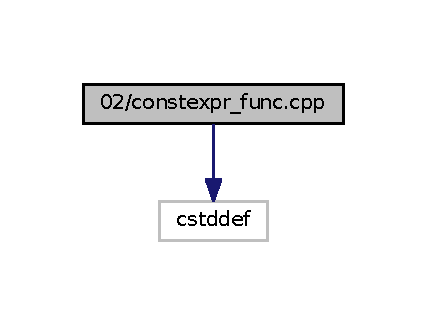
\includegraphics[width=205pt]{constexpr__func_8cpp__incl}
\end{center}
\end{figure}
\subsection*{Functions}
\begin{DoxyCompactItemize}
\item 
constexpr size\+\_\+t \hyperlink{constexpr__func_8cpp_ac1bdbb03b521f0a895628c2fd7d3b650}{bin\+\_\+id\+\_\+gt\+\_\+1} (size\+\_\+t x)
\item 
constexpr size\+\_\+t \hyperlink{constexpr__func_8cpp_a5064165737191e9f5069e4782a7e9a7b}{bin\+\_\+id} (size\+\_\+t x)
\item 
int \hyperlink{constexpr__func_8cpp_a0ddf1224851353fc92bfbff6f499fa97}{main} (int argc, char $\ast$argv\mbox{[}$\,$\mbox{]})
\end{DoxyCompactItemize}


\subsection{Function Documentation}
\index{constexpr\+\_\+func.\+cpp@{constexpr\+\_\+func.\+cpp}!bin\+\_\+id@{bin\+\_\+id}}
\index{bin\+\_\+id@{bin\+\_\+id}!constexpr\+\_\+func.\+cpp@{constexpr\+\_\+func.\+cpp}}
\subsubsection[{\texorpdfstring{bin\+\_\+id(size\+\_\+t x)}{bin_id(size_t x)}}]{\setlength{\rightskip}{0pt plus 5cm}constexpr size\+\_\+t bin\+\_\+id (
\begin{DoxyParamCaption}
\item[{size\+\_\+t}]{x}
\end{DoxyParamCaption}
)}\hypertarget{constexpr__func_8cpp_a5064165737191e9f5069e4782a7e9a7b}{}\label{constexpr__func_8cpp_a5064165737191e9f5069e4782a7e9a7b}
\index{constexpr\+\_\+func.\+cpp@{constexpr\+\_\+func.\+cpp}!bin\+\_\+id\+\_\+gt\+\_\+1@{bin\+\_\+id\+\_\+gt\+\_\+1}}
\index{bin\+\_\+id\+\_\+gt\+\_\+1@{bin\+\_\+id\+\_\+gt\+\_\+1}!constexpr\+\_\+func.\+cpp@{constexpr\+\_\+func.\+cpp}}
\subsubsection[{\texorpdfstring{bin\+\_\+id\+\_\+gt\+\_\+1(size\+\_\+t x)}{bin_id_gt_1(size_t x)}}]{\setlength{\rightskip}{0pt plus 5cm}constexpr size\+\_\+t bin\+\_\+id\+\_\+gt\+\_\+1 (
\begin{DoxyParamCaption}
\item[{size\+\_\+t}]{x}
\end{DoxyParamCaption}
)}\hypertarget{constexpr__func_8cpp_ac1bdbb03b521f0a895628c2fd7d3b650}{}\label{constexpr__func_8cpp_ac1bdbb03b521f0a895628c2fd7d3b650}
\index{constexpr\+\_\+func.\+cpp@{constexpr\+\_\+func.\+cpp}!main@{main}}
\index{main@{main}!constexpr\+\_\+func.\+cpp@{constexpr\+\_\+func.\+cpp}}
\subsubsection[{\texorpdfstring{main(int argc, char $\ast$argv[])}{main(int argc, char *argv[])}}]{\setlength{\rightskip}{0pt plus 5cm}int main (
\begin{DoxyParamCaption}
\item[{int}]{argc, }
\item[{char $\ast$}]{argv\mbox{[}$\,$\mbox{]}}
\end{DoxyParamCaption}
)}\hypertarget{constexpr__func_8cpp_a0ddf1224851353fc92bfbff6f499fa97}{}\label{constexpr__func_8cpp_a0ddf1224851353fc92bfbff6f499fa97}

\hypertarget{02_2ip__loader_8cpp}{}\section{02/ip\+\_\+loader.cpp File Reference}
\label{02_2ip__loader_8cpp}\index{02/ip\+\_\+loader.\+cpp@{02/ip\+\_\+loader.\+cpp}}
{\ttfamily \#include \char`\"{}ip\+\_\+loader.\+h\char`\"{}}\\*
{\ttfamily \#include $<$iostream$>$}\\*
Include dependency graph for ip\+\_\+loader.\+cpp\+:
\nopagebreak
\begin{figure}[H]
\begin{center}
\leavevmode
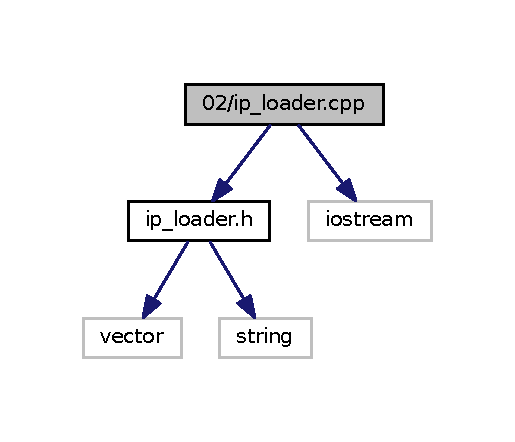
\includegraphics[width=247pt]{02_2ip__loader_8cpp__incl}
\end{center}
\end{figure}

\hypertarget{03__ranges_2ip__loader_8cpp}{}\section{03\+\_\+ranges/ip\+\_\+loader.cpp File Reference}
\label{03__ranges_2ip__loader_8cpp}\index{03\+\_\+ranges/ip\+\_\+loader.\+cpp@{03\+\_\+ranges/ip\+\_\+loader.\+cpp}}
{\ttfamily \#include \char`\"{}ip\+\_\+loader.\+h\char`\"{}}\\*
{\ttfamily \#include $<$iostream$>$}\\*
{\ttfamily \#include $<$vector$>$}\\*
{\ttfamily \#include $<$string$>$}\\*
{\ttfamily \#include $<$meta/meta.\+hpp$>$}\\*
{\ttfamily \#include $<$range/v3/algorithm/sort.\+hpp$>$}\\*
{\ttfamily \#include $<$range/v3/all.\+hpp$>$}\\*
{\ttfamily \#include $<$range/v3/algorithm.\+hpp$>$}\\*
{\ttfamily \#include $<$range/v3/iterator.\+hpp$>$}\\*
{\ttfamily \#include $<$range/v3/view/split.\+hpp$>$}\\*
Include dependency graph for ip\+\_\+loader.\+cpp\+:
\nopagebreak
\begin{figure}[H]
\begin{center}
\leavevmode
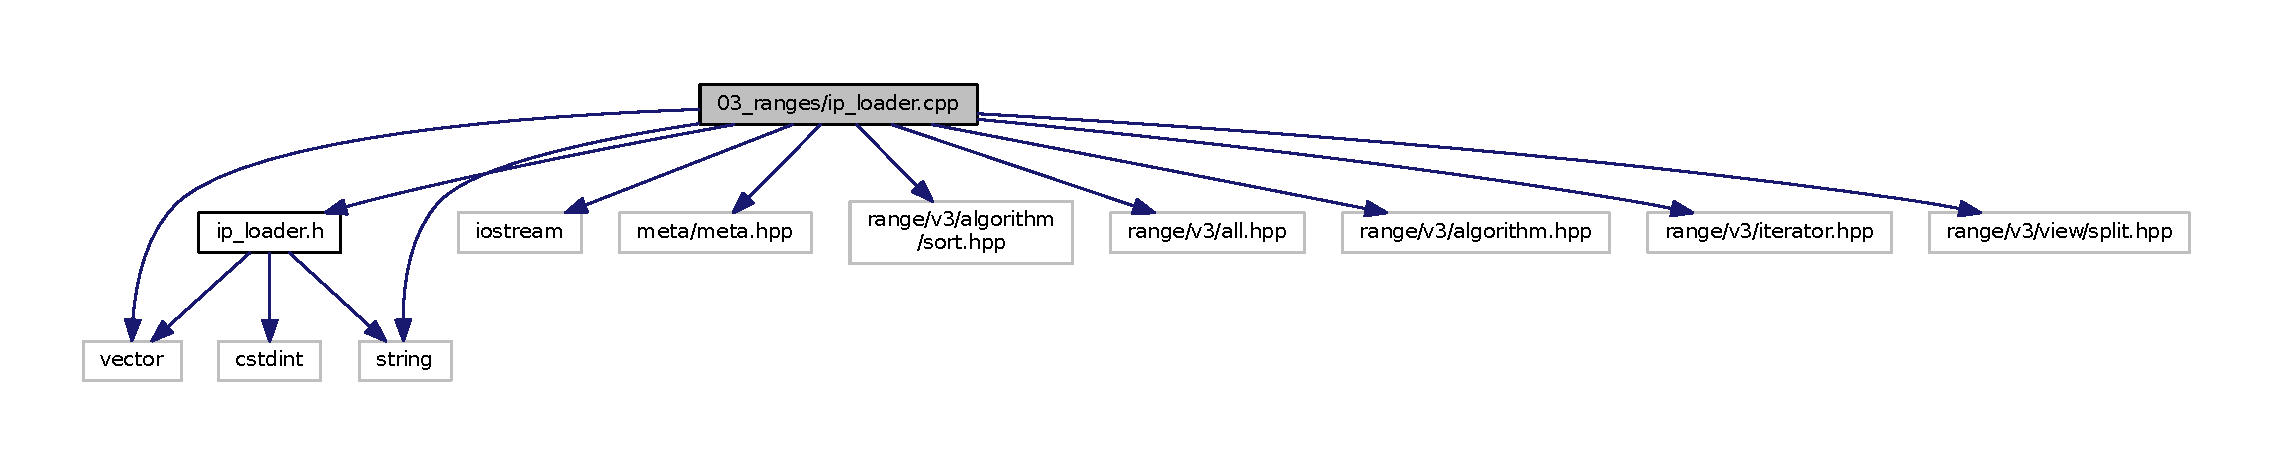
\includegraphics[width=350pt]{03__ranges_2ip__loader_8cpp__incl}
\end{center}
\end{figure}

\hypertarget{02_2ip__loader_8h}{}\section{02/ip\+\_\+loader.h File Reference}
\label{02_2ip__loader_8h}\index{02/ip\+\_\+loader.\+h@{02/ip\+\_\+loader.\+h}}
{\ttfamily \#include $<$vector$>$}\\*
{\ttfamily \#include $<$string$>$}\\*
Include dependency graph for ip\+\_\+loader.\+h\+:
\nopagebreak
\begin{figure}[H]
\begin{center}
\leavevmode
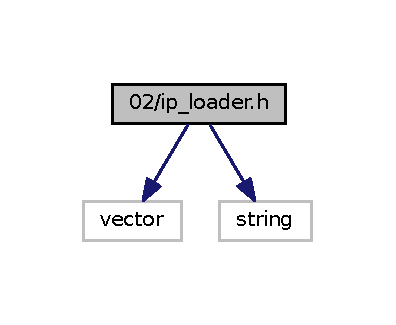
\includegraphics[width=190pt]{02_2ip__loader_8h__incl}
\end{center}
\end{figure}
This graph shows which files directly or indirectly include this file\+:
\nopagebreak
\begin{figure}[H]
\begin{center}
\leavevmode
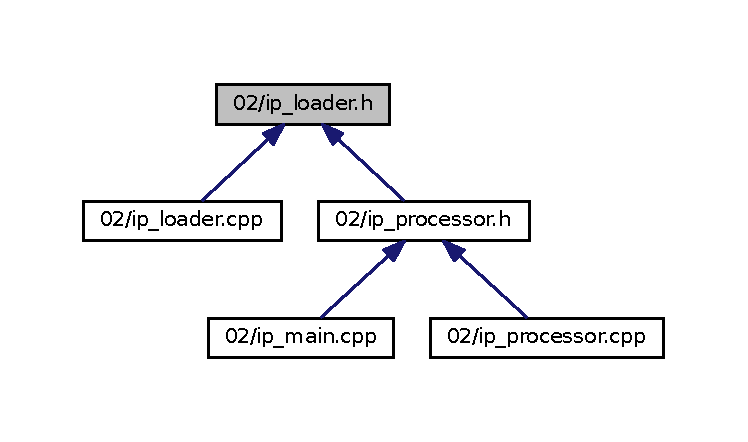
\includegraphics[width=350pt]{02_2ip__loader_8h__dep__incl}
\end{center}
\end{figure}
\subsection*{Classes}
\begin{DoxyCompactItemize}
\item 
class \hyperlink{classIpDataLoader}{Ip\+Data\+Loader}
\end{DoxyCompactItemize}
\subsection*{Typedefs}
\begin{DoxyCompactItemize}
\item 
using \hyperlink{02_2ip__loader_8h_ad6543533a9d8728e8ffbb208890f492e}{vec\+\_\+str} = vector$<$ string $>$
\end{DoxyCompactItemize}


\subsection{Typedef Documentation}
\index{02/ip\+\_\+loader.\+h@{02/ip\+\_\+loader.\+h}!vec\+\_\+str@{vec\+\_\+str}}
\index{vec\+\_\+str@{vec\+\_\+str}!02/ip\+\_\+loader.\+h@{02/ip\+\_\+loader.\+h}}
\subsubsection[{\texorpdfstring{vec\+\_\+str}{vec_str}}]{\setlength{\rightskip}{0pt plus 5cm}using {\bf vec\+\_\+str} =  vector$<$string$>$}\hypertarget{02_2ip__loader_8h_ad6543533a9d8728e8ffbb208890f492e}{}\label{02_2ip__loader_8h_ad6543533a9d8728e8ffbb208890f492e}

\hypertarget{03__ranges_2ip__loader_8h}{}\section{03\+\_\+ranges/ip\+\_\+loader.h File Reference}
\label{03__ranges_2ip__loader_8h}\index{03\+\_\+ranges/ip\+\_\+loader.\+h@{03\+\_\+ranges/ip\+\_\+loader.\+h}}
{\ttfamily \#include $<$vector$>$}\\*
{\ttfamily \#include $<$string$>$}\\*
{\ttfamily \#include $<$cstdint$>$}\\*
Include dependency graph for ip\+\_\+loader.\+h\+:
\nopagebreak
\begin{figure}[H]
\begin{center}
\leavevmode
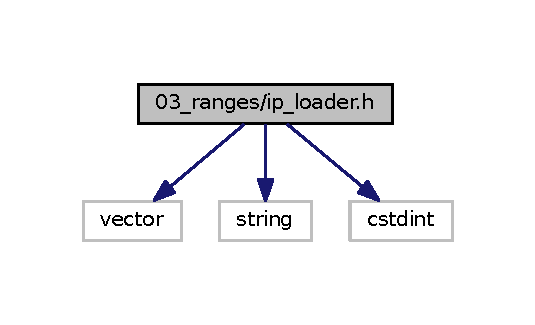
\includegraphics[width=257pt]{03__ranges_2ip__loader_8h__incl}
\end{center}
\end{figure}
This graph shows which files directly or indirectly include this file\+:
\nopagebreak
\begin{figure}[H]
\begin{center}
\leavevmode
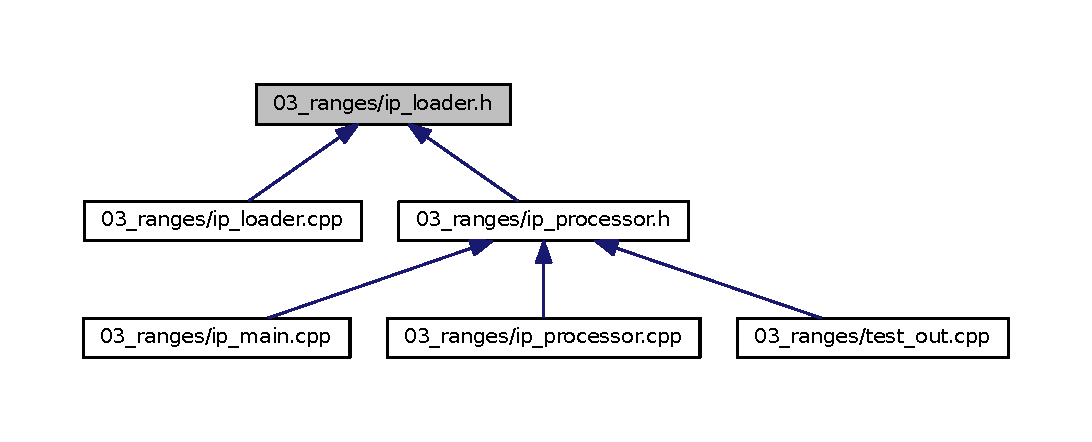
\includegraphics[width=350pt]{03__ranges_2ip__loader_8h__dep__incl}
\end{center}
\end{figure}
\subsection*{Classes}
\begin{DoxyCompactItemize}
\item 
class \hyperlink{classIpDataLoader}{Ip\+Data\+Loader}
\end{DoxyCompactItemize}
\subsection*{Typedefs}
\begin{DoxyCompactItemize}
\item 
using \hyperlink{03__ranges_2ip__loader_8h_adf9c1fa121650f19b895ecb6217615f2}{vec\+\_\+ui8} = vector$<$ uint8\+\_\+t $>$
\end{DoxyCompactItemize}


\subsection{Typedef Documentation}
\index{03\+\_\+ranges/ip\+\_\+loader.\+h@{03\+\_\+ranges/ip\+\_\+loader.\+h}!vec\+\_\+ui8@{vec\+\_\+ui8}}
\index{vec\+\_\+ui8@{vec\+\_\+ui8}!03\+\_\+ranges/ip\+\_\+loader.\+h@{03\+\_\+ranges/ip\+\_\+loader.\+h}}
\subsubsection[{\texorpdfstring{vec\+\_\+ui8}{vec_ui8}}]{\setlength{\rightskip}{0pt plus 5cm}using {\bf vec\+\_\+ui8} =  vector$<$uint8\+\_\+t$>$}\hypertarget{03__ranges_2ip__loader_8h_adf9c1fa121650f19b895ecb6217615f2}{}\label{03__ranges_2ip__loader_8h_adf9c1fa121650f19b895ecb6217615f2}

\hypertarget{02_2ip__main_8cpp}{}\section{02/ip\+\_\+main.cpp File Reference}
\label{02_2ip__main_8cpp}\index{02/ip\+\_\+main.\+cpp@{02/ip\+\_\+main.\+cpp}}
{\ttfamily \#include \char`\"{}ip\+\_\+processor.\+h\char`\"{}}\\*
{\ttfamily \#include $<$iostream$>$}\\*
{\ttfamily \#include $<$memory$>$}\\*
Include dependency graph for ip\+\_\+main.\+cpp\+:
\nopagebreak
\begin{figure}[H]
\begin{center}
\leavevmode
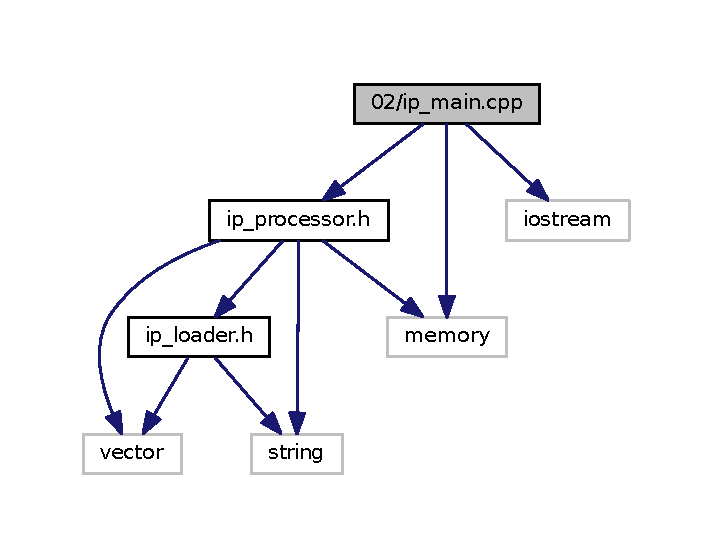
\includegraphics[width=342pt]{02_2ip__main_8cpp__incl}
\end{center}
\end{figure}
\subsection*{Functions}
\begin{DoxyCompactItemize}
\item 
int \hyperlink{02_2ip__main_8cpp_a0ddf1224851353fc92bfbff6f499fa97}{main} (int argc, char $\ast$argv\mbox{[}$\,$\mbox{]})
\end{DoxyCompactItemize}


\subsection{Function Documentation}
\index{02/ip\+\_\+main.\+cpp@{02/ip\+\_\+main.\+cpp}!main@{main}}
\index{main@{main}!02/ip\+\_\+main.\+cpp@{02/ip\+\_\+main.\+cpp}}
\subsubsection[{\texorpdfstring{main(int argc, char $\ast$argv[])}{main(int argc, char *argv[])}}]{\setlength{\rightskip}{0pt plus 5cm}int main (
\begin{DoxyParamCaption}
\item[{int}]{argc, }
\item[{char $\ast$}]{argv\mbox{[}$\,$\mbox{]}}
\end{DoxyParamCaption}
)}\hypertarget{02_2ip__main_8cpp_a0ddf1224851353fc92bfbff6f499fa97}{}\label{02_2ip__main_8cpp_a0ddf1224851353fc92bfbff6f499fa97}

\hypertarget{03__ranges_2ip__main_8cpp}{}\section{03\+\_\+ranges/ip\+\_\+main.cpp File Reference}
\label{03__ranges_2ip__main_8cpp}\index{03\+\_\+ranges/ip\+\_\+main.\+cpp@{03\+\_\+ranges/ip\+\_\+main.\+cpp}}
{\ttfamily \#include \char`\"{}ip\+\_\+processor.\+h\char`\"{}}\\*
{\ttfamily \#include $<$iostream$>$}\\*
{\ttfamily \#include $<$memory$>$}\\*
Include dependency graph for ip\+\_\+main.\+cpp\+:
\nopagebreak
\begin{figure}[H]
\begin{center}
\leavevmode
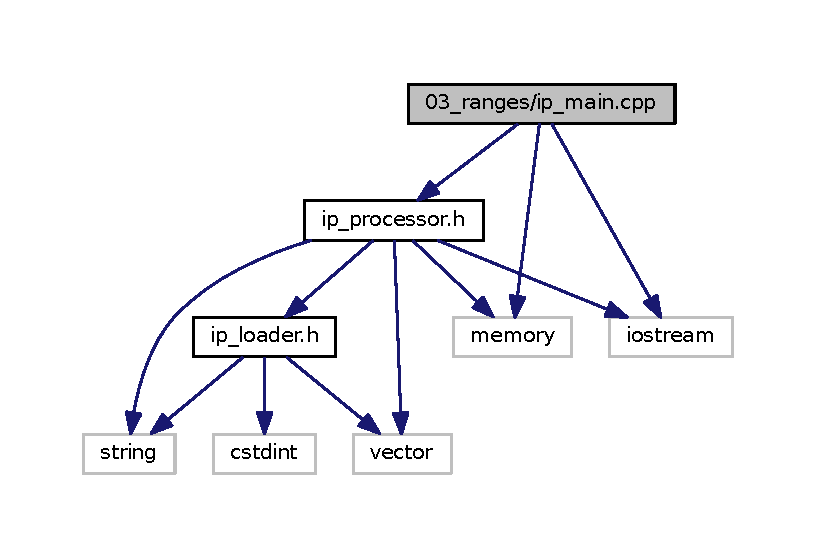
\includegraphics[width=350pt]{03__ranges_2ip__main_8cpp__incl}
\end{center}
\end{figure}
\subsection*{Functions}
\begin{DoxyCompactItemize}
\item 
int \hyperlink{03__ranges_2ip__main_8cpp_a0ddf1224851353fc92bfbff6f499fa97}{main} (int argc, char $\ast$argv\mbox{[}$\,$\mbox{]})
\end{DoxyCompactItemize}


\subsection{Function Documentation}
\index{03\+\_\+ranges/ip\+\_\+main.\+cpp@{03\+\_\+ranges/ip\+\_\+main.\+cpp}!main@{main}}
\index{main@{main}!03\+\_\+ranges/ip\+\_\+main.\+cpp@{03\+\_\+ranges/ip\+\_\+main.\+cpp}}
\subsubsection[{\texorpdfstring{main(int argc, char $\ast$argv[])}{main(int argc, char *argv[])}}]{\setlength{\rightskip}{0pt plus 5cm}int main (
\begin{DoxyParamCaption}
\item[{int}]{argc, }
\item[{char $\ast$}]{argv\mbox{[}$\,$\mbox{]}}
\end{DoxyParamCaption}
)}\hypertarget{03__ranges_2ip__main_8cpp_a0ddf1224851353fc92bfbff6f499fa97}{}\label{03__ranges_2ip__main_8cpp_a0ddf1224851353fc92bfbff6f499fa97}

\hypertarget{02_2ip__processor_8cpp}{}\section{02/ip\+\_\+processor.cpp File Reference}
\label{02_2ip__processor_8cpp}\index{02/ip\+\_\+processor.\+cpp@{02/ip\+\_\+processor.\+cpp}}
{\ttfamily \#include \char`\"{}ip\+\_\+processor.\+h\char`\"{}}\\*
{\ttfamily \#include $<$iostream$>$}\\*
{\ttfamily \#include $<$algorithm$>$}\\*
{\ttfamily \#include $<$iterator$>$}\\*
{\ttfamily \#include $<$ostream$>$}\\*
Include dependency graph for ip\+\_\+processor.\+cpp\+:
\nopagebreak
\begin{figure}[H]
\begin{center}
\leavevmode
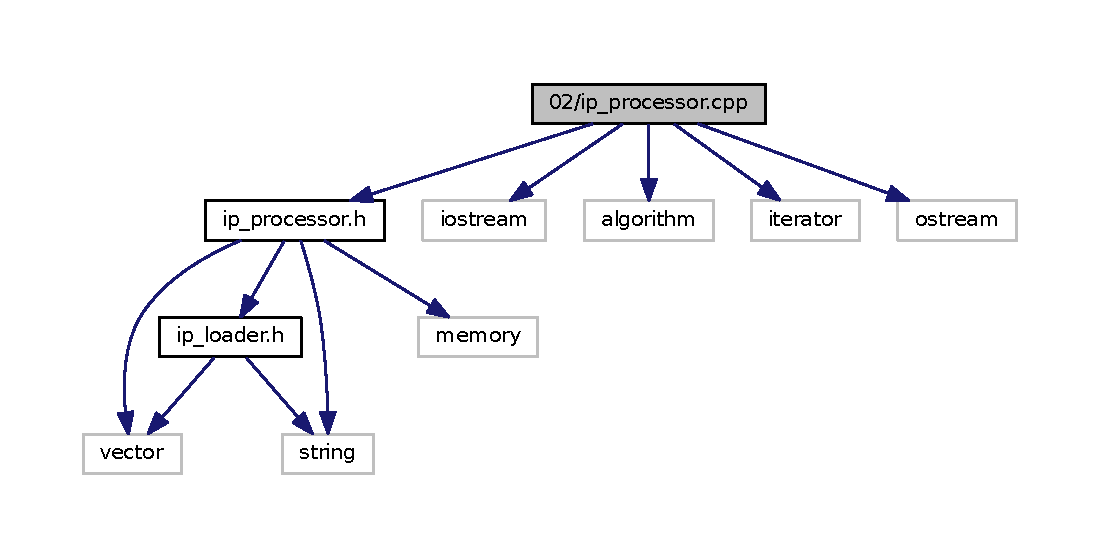
\includegraphics[width=350pt]{02_2ip__processor_8cpp__incl}
\end{center}
\end{figure}
\subsection*{Namespaces}
\begin{DoxyCompactItemize}
\item 
 \hyperlink{namespacestd}{std}
\end{DoxyCompactItemize}
\subsection*{Functions}
\begin{DoxyCompactItemize}
\item 
std\+::ostream \& \hyperlink{namespacestd_a985b65a9256bbd1a753db3025f101175}{std\+::operator$<$$<$} (std\+::ostream \&os, const std\+::vector$<$ std\+::string $>$ \&vs)
\item 
{\footnotesize template$<$typename Predicate $>$ }\\void \hyperlink{02_2ip__processor_8cpp_a6cb34919eb988bbeb21974a9623a7706}{print\+\_\+any\+\_\+condition} (const vector$<$ \hyperlink{02_2ip__loader_8h_ad6543533a9d8728e8ffbb208890f492e}{vec\+\_\+str} $>$ \&ippool, Predicate P1)
\end{DoxyCompactItemize}


\subsection{Function Documentation}
\index{02/ip\+\_\+processor.\+cpp@{02/ip\+\_\+processor.\+cpp}!print\+\_\+any\+\_\+condition@{print\+\_\+any\+\_\+condition}}
\index{print\+\_\+any\+\_\+condition@{print\+\_\+any\+\_\+condition}!02/ip\+\_\+processor.\+cpp@{02/ip\+\_\+processor.\+cpp}}
\subsubsection[{\texorpdfstring{print\+\_\+any\+\_\+condition(const vector$<$ vec\+\_\+str $>$ \&ippool, Predicate P1)}{print_any_condition(const vector< vec_str > &ippool, Predicate P1)}}]{\setlength{\rightskip}{0pt plus 5cm}template$<$typename Predicate $>$ void print\+\_\+any\+\_\+condition (
\begin{DoxyParamCaption}
\item[{const vector$<$ {\bf vec\+\_\+str} $>$ \&}]{ippool, }
\item[{Predicate}]{P1}
\end{DoxyParamCaption}
)}\hypertarget{02_2ip__processor_8cpp_a6cb34919eb988bbeb21974a9623a7706}{}\label{02_2ip__processor_8cpp_a6cb34919eb988bbeb21974a9623a7706}

\hypertarget{03__ranges_2ip__processor_8cpp}{}\section{03\+\_\+ranges/ip\+\_\+processor.cpp File Reference}
\label{03__ranges_2ip__processor_8cpp}\index{03\+\_\+ranges/ip\+\_\+processor.\+cpp@{03\+\_\+ranges/ip\+\_\+processor.\+cpp}}
{\ttfamily \#include \char`\"{}ip\+\_\+processor.\+h\char`\"{}}\\*
{\ttfamily \#include $<$iostream$>$}\\*
{\ttfamily \#include $<$algorithm$>$}\\*
{\ttfamily \#include $<$iterator$>$}\\*
{\ttfamily \#include $<$ostream$>$}\\*
{\ttfamily \#include $<$range/v3/all.\+hpp$>$}\\*
{\ttfamily \#include $<$range/v3/algorithm/sort.\+hpp$>$}\\*
Include dependency graph for ip\+\_\+processor.\+cpp\+:
\nopagebreak
\begin{figure}[H]
\begin{center}
\leavevmode
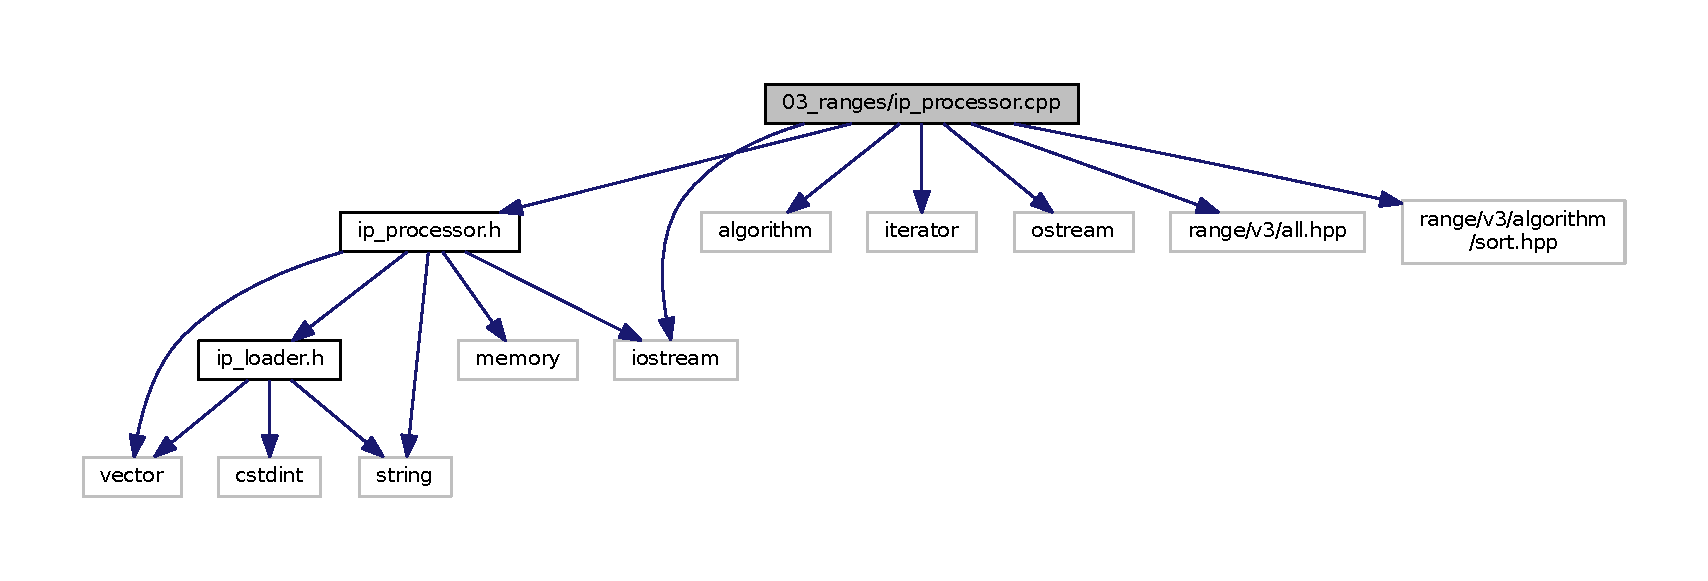
\includegraphics[width=350pt]{03__ranges_2ip__processor_8cpp__incl}
\end{center}
\end{figure}
\subsection*{Namespaces}
\begin{DoxyCompactItemize}
\item 
 \hyperlink{namespacestd}{std}
\end{DoxyCompactItemize}
\subsection*{Functions}
\begin{DoxyCompactItemize}
\item 
std\+::ostream \& \hyperlink{namespacestd_abb27abe27271b88570c789062cb2089a}{std\+::operator$<$$<$} (std\+::ostream \&os, const \hyperlink{03__ranges_2ip__loader_8h_adf9c1fa121650f19b895ecb6217615f2}{vec\+\_\+ui8} \&vs)
\item 
void \hyperlink{03__ranges_2ip__processor_8cpp_a79396c609a09a70fc948375f89e75a35}{print} (const vector$<$ \hyperlink{03__ranges_2ip__loader_8h_adf9c1fa121650f19b895ecb6217615f2}{vec\+\_\+ui8} $>$ \&ippool, std\+::ostream \&output)
\end{DoxyCompactItemize}


\subsection{Function Documentation}
\index{03\+\_\+ranges/ip\+\_\+processor.\+cpp@{03\+\_\+ranges/ip\+\_\+processor.\+cpp}!print@{print}}
\index{print@{print}!03\+\_\+ranges/ip\+\_\+processor.\+cpp@{03\+\_\+ranges/ip\+\_\+processor.\+cpp}}
\subsubsection[{\texorpdfstring{print(const vector$<$ vec\+\_\+ui8 $>$ \&ippool, std\+::ostream \&output)}{print(const vector< vec_ui8 > &ippool, std::ostream &output)}}]{\setlength{\rightskip}{0pt plus 5cm}void print (
\begin{DoxyParamCaption}
\item[{const vector$<$ {\bf vec\+\_\+ui8} $>$ \&}]{ippool, }
\item[{std\+::ostream \&}]{output}
\end{DoxyParamCaption}
)}\hypertarget{03__ranges_2ip__processor_8cpp_a79396c609a09a70fc948375f89e75a35}{}\label{03__ranges_2ip__processor_8cpp_a79396c609a09a70fc948375f89e75a35}

\hypertarget{02_2ip__processor_8h}{}\section{02/ip\+\_\+processor.h File Reference}
\label{02_2ip__processor_8h}\index{02/ip\+\_\+processor.\+h@{02/ip\+\_\+processor.\+h}}
{\ttfamily \#include \char`\"{}ip\+\_\+loader.\+h\char`\"{}}\\*
{\ttfamily \#include $<$memory$>$}\\*
{\ttfamily \#include $<$vector$>$}\\*
{\ttfamily \#include $<$string$>$}\\*
Include dependency graph for ip\+\_\+processor.\+h\+:
\nopagebreak
\begin{figure}[H]
\begin{center}
\leavevmode
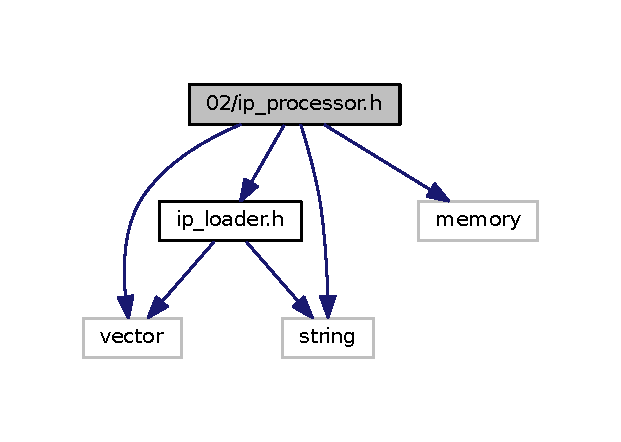
\includegraphics[width=298pt]{02_2ip__processor_8h__incl}
\end{center}
\end{figure}
This graph shows which files directly or indirectly include this file\+:
\nopagebreak
\begin{figure}[H]
\begin{center}
\leavevmode
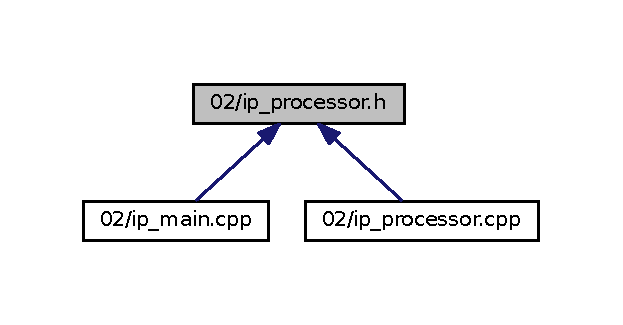
\includegraphics[width=299pt]{02_2ip__processor_8h__dep__incl}
\end{center}
\end{figure}
\subsection*{Classes}
\begin{DoxyCompactItemize}
\item 
class \hyperlink{classIpProcessor}{Ip\+Processor}
\end{DoxyCompactItemize}

\hypertarget{03__ranges_2ip__processor_8h}{}\section{03\+\_\+ranges/ip\+\_\+processor.h File Reference}
\label{03__ranges_2ip__processor_8h}\index{03\+\_\+ranges/ip\+\_\+processor.\+h@{03\+\_\+ranges/ip\+\_\+processor.\+h}}
{\ttfamily \#include \char`\"{}ip\+\_\+loader.\+h\char`\"{}}\\*
{\ttfamily \#include $<$memory$>$}\\*
{\ttfamily \#include $<$vector$>$}\\*
{\ttfamily \#include $<$string$>$}\\*
{\ttfamily \#include $<$iostream$>$}\\*
Include dependency graph for ip\+\_\+processor.\+h\+:
\nopagebreak
\begin{figure}[H]
\begin{center}
\leavevmode
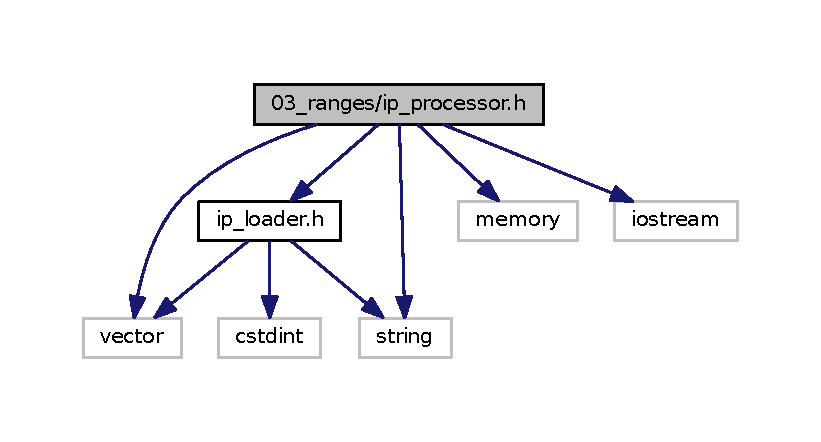
\includegraphics[width=350pt]{03__ranges_2ip__processor_8h__incl}
\end{center}
\end{figure}
This graph shows which files directly or indirectly include this file\+:
\nopagebreak
\begin{figure}[H]
\begin{center}
\leavevmode
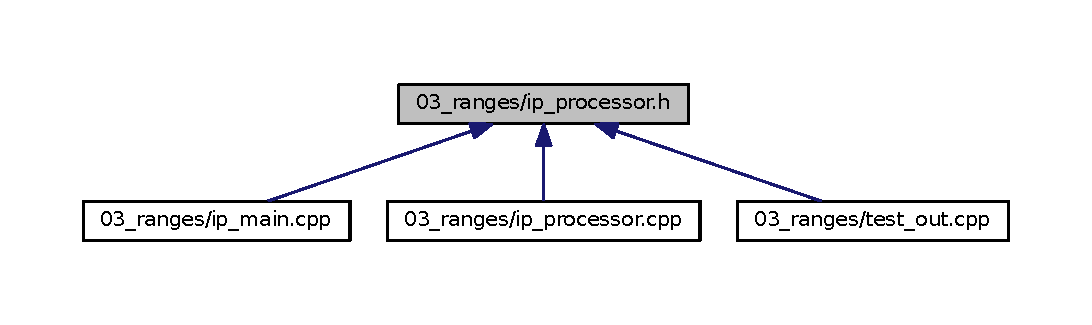
\includegraphics[width=350pt]{03__ranges_2ip__processor_8h__dep__incl}
\end{center}
\end{figure}
\subsection*{Classes}
\begin{DoxyCompactItemize}
\item 
class \hyperlink{classIpProcessor}{Ip\+Processor}
\end{DoxyCompactItemize}

\hypertarget{cstm__pair_8hpp}{}\section{02\+\_\+tuple/cstm\+\_\+pair.hpp File Reference}
\label{cstm__pair_8hpp}\index{02\+\_\+tuple/cstm\+\_\+pair.\+hpp@{02\+\_\+tuple/cstm\+\_\+pair.\+hpp}}
{\ttfamily \#include $<$algorithm$>$}\\*
{\ttfamily \#include $<$iostream$>$}\\*
{\ttfamily \#include $<$type\+\_\+traits$>$}\\*
Include dependency graph for cstm\+\_\+pair.\+hpp\+:
\nopagebreak
\begin{figure}[H]
\begin{center}
\leavevmode
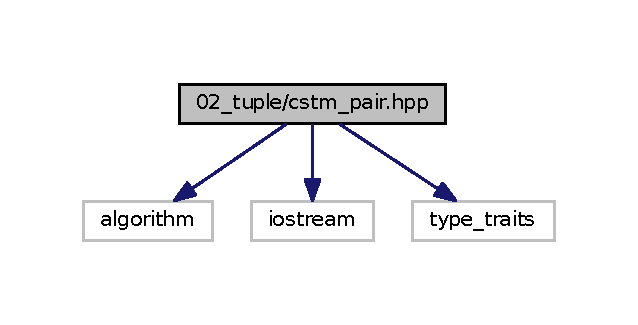
\includegraphics[width=306pt]{cstm__pair_8hpp__incl}
\end{center}
\end{figure}
This graph shows which files directly or indirectly include this file\+:
\nopagebreak
\begin{figure}[H]
\begin{center}
\leavevmode
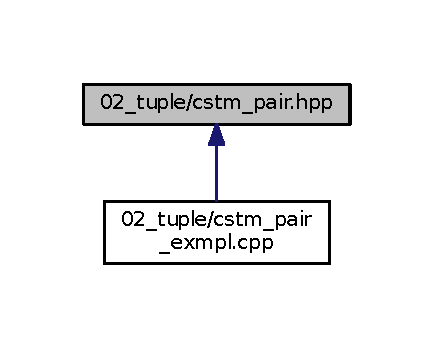
\includegraphics[width=208pt]{cstm__pair_8hpp__dep__incl}
\end{center}
\end{figure}
\subsection*{Classes}
\begin{DoxyCompactItemize}
\item 
class \hyperlink{classCustomPair}{Custom\+Pair$<$ T1, U2 $>$}
\item 
class \hyperlink{classCustomPair_3_01T1_01_6_00_01U2_01_6_01_4}{Custom\+Pair$<$ T1 \&, U2 \& $>$}
\end{DoxyCompactItemize}
\subsection*{Functions}
\begin{DoxyCompactItemize}
\item 
{\footnotesize template$<$typename T1 , typename U2 $>$ }\\std\+::ostream \& \hyperlink{cstm__pair_8hpp_a9e995341e5de1cd5b91e01ca94b519c4}{operator$<$$<$} (std\+::ostream \&os, const \hyperlink{classCustomPair}{Custom\+Pair}$<$ T1, U2 $>$ \&rhs\+\_\+pr)
\item 
{\footnotesize template$<$std\+::size\+\_\+t n, typename T1 , typename U2 $>$ }\\std\+::enable\+\_\+if$<$ n==0, T1 $>$\+::type \& \hyperlink{cstm__pair_8hpp_aefe0ca04fd4eca3c7e2e7629d28786eb}{get} (\hyperlink{classCustomPair}{Custom\+Pair}$<$ T1, U2 $>$ \&cstm\+\_\+pair)
\item 
{\footnotesize template$<$std\+::size\+\_\+t n, typename T1 , typename U2 $>$ }\\std\+::enable\+\_\+if$<$ n==1, U2 $>$\+::type \& \hyperlink{cstm__pair_8hpp_a97080eade9568466123a90d375487f2f}{get} (\hyperlink{classCustomPair}{Custom\+Pair}$<$ T1, U2 $>$ \&cstm\+\_\+pair)
\item 
{\footnotesize template$<$typename T1 , typename U2 $>$ }\\std\+::ostream \& \hyperlink{cstm__pair_8hpp_aa7814abf8ff90cf37d6a8c538977263e}{operator$<$$<$} (std\+::ostream \&os, const \hyperlink{classCustomPair}{Custom\+Pair}$<$ T1 \&, U2 \& $>$ \&rhs\+\_\+pr)
\item 
{\footnotesize template$<$typename T1 , typename U2 $>$ }\\\hyperlink{classCustomPair}{Custom\+Pair}$<$ T1 \&, U2 \& $>$ \hyperlink{cstm__pair_8hpp_a77134479457c9e9914f95c32359b4ac0}{custom\+\_\+tie} (T1 \&f, U2 \&s)
\item 
{\footnotesize template$<$typename T1 , typename U2 $>$ }\\\hyperlink{classCustomPair}{Custom\+Pair}$<$ T1, U2 $>$ \hyperlink{cstm__pair_8hpp_ac248ca822921e4d7885334626cb7e463}{make\+\_\+custom\+\_\+pair} (T1 f, U2 s)
\end{DoxyCompactItemize}


\subsection{Function Documentation}
\index{cstm\+\_\+pair.\+hpp@{cstm\+\_\+pair.\+hpp}!custom\+\_\+tie@{custom\+\_\+tie}}
\index{custom\+\_\+tie@{custom\+\_\+tie}!cstm\+\_\+pair.\+hpp@{cstm\+\_\+pair.\+hpp}}
\subsubsection[{\texorpdfstring{custom\+\_\+tie(\+T1 \&f, U2 \&s)}{custom_tie(T1 &f, U2 &s)}}]{\setlength{\rightskip}{0pt plus 5cm}template$<$typename T1 , typename U2 $>$ {\bf Custom\+Pair}$<$ T1 \&, U2 \& $>$ custom\+\_\+tie (
\begin{DoxyParamCaption}
\item[{T1 \&}]{f, }
\item[{U2 \&}]{s}
\end{DoxyParamCaption}
)}\hypertarget{cstm__pair_8hpp_a77134479457c9e9914f95c32359b4ac0}{}\label{cstm__pair_8hpp_a77134479457c9e9914f95c32359b4ac0}
\index{cstm\+\_\+pair.\+hpp@{cstm\+\_\+pair.\+hpp}!get@{get}}
\index{get@{get}!cstm\+\_\+pair.\+hpp@{cstm\+\_\+pair.\+hpp}}
\subsubsection[{\texorpdfstring{get(\+Custom\+Pair$<$ T1, U2 $>$ \&cstm\+\_\+pair)}{get(CustomPair< T1, U2 > &cstm_pair)}}]{\setlength{\rightskip}{0pt plus 5cm}template$<$std\+::size\+\_\+t n, typename T1 , typename U2 $>$ std\+::enable\+\_\+if$<$ n==0, T1 $>$\+::type \& get (
\begin{DoxyParamCaption}
\item[{{\bf Custom\+Pair}$<$ T1, U2 $>$ \&}]{cstm\+\_\+pair}
\end{DoxyParamCaption}
)}\hypertarget{cstm__pair_8hpp_aefe0ca04fd4eca3c7e2e7629d28786eb}{}\label{cstm__pair_8hpp_aefe0ca04fd4eca3c7e2e7629d28786eb}
\index{cstm\+\_\+pair.\+hpp@{cstm\+\_\+pair.\+hpp}!get@{get}}
\index{get@{get}!cstm\+\_\+pair.\+hpp@{cstm\+\_\+pair.\+hpp}}
\subsubsection[{\texorpdfstring{get(\+Custom\+Pair$<$ T1, U2 $>$ \&cstm\+\_\+pair)}{get(CustomPair< T1, U2 > &cstm_pair)}}]{\setlength{\rightskip}{0pt plus 5cm}template$<$std\+::size\+\_\+t n, typename T1 , typename U2 $>$ std\+::enable\+\_\+if$<$ n==1, U2 $>$\+::type \& get (
\begin{DoxyParamCaption}
\item[{{\bf Custom\+Pair}$<$ T1, U2 $>$ \&}]{cstm\+\_\+pair}
\end{DoxyParamCaption}
)}\hypertarget{cstm__pair_8hpp_a97080eade9568466123a90d375487f2f}{}\label{cstm__pair_8hpp_a97080eade9568466123a90d375487f2f}
\index{cstm\+\_\+pair.\+hpp@{cstm\+\_\+pair.\+hpp}!make\+\_\+custom\+\_\+pair@{make\+\_\+custom\+\_\+pair}}
\index{make\+\_\+custom\+\_\+pair@{make\+\_\+custom\+\_\+pair}!cstm\+\_\+pair.\+hpp@{cstm\+\_\+pair.\+hpp}}
\subsubsection[{\texorpdfstring{make\+\_\+custom\+\_\+pair(\+T1 f, U2 s)}{make_custom_pair(T1 f, U2 s)}}]{\setlength{\rightskip}{0pt plus 5cm}template$<$typename T1 , typename U2 $>$ {\bf Custom\+Pair}$<$T1, U2$>$ make\+\_\+custom\+\_\+pair (
\begin{DoxyParamCaption}
\item[{T1}]{f, }
\item[{U2}]{s}
\end{DoxyParamCaption}
)}\hypertarget{cstm__pair_8hpp_ac248ca822921e4d7885334626cb7e463}{}\label{cstm__pair_8hpp_ac248ca822921e4d7885334626cb7e463}
\index{cstm\+\_\+pair.\+hpp@{cstm\+\_\+pair.\+hpp}!operator$<$$<$@{operator$<$$<$}}
\index{operator$<$$<$@{operator$<$$<$}!cstm\+\_\+pair.\+hpp@{cstm\+\_\+pair.\+hpp}}
\subsubsection[{\texorpdfstring{operator$<$$<$(std\+::ostream \&os, const Custom\+Pair$<$ T1, U2 $>$ \&rhs\+\_\+pr)}{operator<<(std::ostream &os, const CustomPair< T1, U2 > &rhs_pr)}}]{\setlength{\rightskip}{0pt plus 5cm}template$<$typename T1 , typename U2 $>$ std\+::ostream \& operator$<$$<$ (
\begin{DoxyParamCaption}
\item[{std\+::ostream \&}]{os, }
\item[{const {\bf Custom\+Pair}$<$ T1, U2 $>$ \&}]{rhs\+\_\+pr}
\end{DoxyParamCaption}
)}\hypertarget{cstm__pair_8hpp_a9e995341e5de1cd5b91e01ca94b519c4}{}\label{cstm__pair_8hpp_a9e995341e5de1cd5b91e01ca94b519c4}
\index{cstm\+\_\+pair.\+hpp@{cstm\+\_\+pair.\+hpp}!operator$<$$<$@{operator$<$$<$}}
\index{operator$<$$<$@{operator$<$$<$}!cstm\+\_\+pair.\+hpp@{cstm\+\_\+pair.\+hpp}}
\subsubsection[{\texorpdfstring{operator$<$$<$(std\+::ostream \&os, const Custom\+Pair$<$ T1 \&, U2 \& $>$ \&rhs\+\_\+pr)}{operator<<(std::ostream &os, const CustomPair< T1 &, U2 & > &rhs_pr)}}]{\setlength{\rightskip}{0pt plus 5cm}template$<$typename T1 , typename U2 $>$ std\+::ostream \& operator$<$$<$ (
\begin{DoxyParamCaption}
\item[{std\+::ostream \&}]{os, }
\item[{const {\bf Custom\+Pair}$<$ T1 \&, U2 \& $>$ \&}]{rhs\+\_\+pr}
\end{DoxyParamCaption}
)}\hypertarget{cstm__pair_8hpp_aa7814abf8ff90cf37d6a8c538977263e}{}\label{cstm__pair_8hpp_aa7814abf8ff90cf37d6a8c538977263e}

\hypertarget{cstm__pair__2_8hpp}{}\section{02\+\_\+tuple/cstm\+\_\+pair\+\_\+2.hpp File Reference}
\label{cstm__pair__2_8hpp}\index{02\+\_\+tuple/cstm\+\_\+pair\+\_\+2.\+hpp@{02\+\_\+tuple/cstm\+\_\+pair\+\_\+2.\+hpp}}
{\ttfamily \#include $<$algorithm$>$}\\*
{\ttfamily \#include $<$iostream$>$}\\*
{\ttfamily \#include $<$type\+\_\+traits$>$}\\*
Include dependency graph for cstm\+\_\+pair\+\_\+2.\+hpp\+:
\nopagebreak
\begin{figure}[H]
\begin{center}
\leavevmode
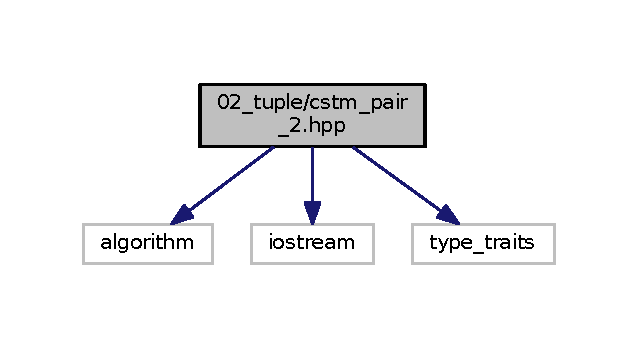
\includegraphics[width=306pt]{cstm__pair__2_8hpp__incl}
\end{center}
\end{figure}
This graph shows which files directly or indirectly include this file\+:
\nopagebreak
\begin{figure}[H]
\begin{center}
\leavevmode
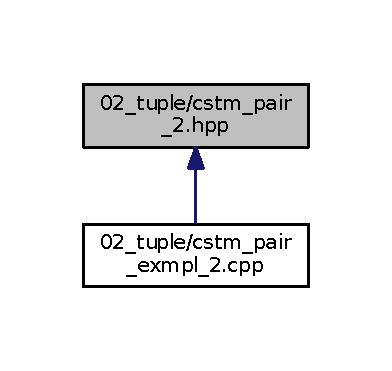
\includegraphics[width=188pt]{cstm__pair__2_8hpp__dep__incl}
\end{center}
\end{figure}
\subsection*{Classes}
\begin{DoxyCompactItemize}
\item 
class \hyperlink{classCustomPair2}{Custom\+Pair2$<$ T1, U2 $>$}
\end{DoxyCompactItemize}
\subsection*{Functions}
\begin{DoxyCompactItemize}
\item 
{\footnotesize template$<$typename T1 , typename U2 $>$ }\\std\+::ostream \& \hyperlink{cstm__pair__2_8hpp_a02d1c656174a47097d94b709c0b9a12c}{operator$<$$<$} (std\+::ostream \&os, const \hyperlink{classCustomPair2}{Custom\+Pair2}$<$ T1, U2 $>$ \&rhs\+\_\+pr)
\item 
{\footnotesize template$<$typename T1 , typename U2 $>$ }\\auto \hyperlink{cstm__pair__2_8hpp_afcf876dab5036d814a6ed52d0356ecab}{custom\+\_\+pair\+\_\+tie} (T1 \&\&f, U2 \&\&s)
\item 
{\footnotesize template$<$std\+::size\+\_\+t n, typename T1 , typename U2 $>$ }\\std\+::enable\+\_\+if$<$ n==0, T1 $>$\+::type \& \hyperlink{cstm__pair__2_8hpp_a4986bf935098b9486b29507d194f6dd5}{get} (\hyperlink{classCustomPair2}{Custom\+Pair2}$<$ T1, U2 $>$ \&cstm\+\_\+pair)
\item 
{\footnotesize template$<$std\+::size\+\_\+t n, typename T1 , typename U2 $>$ }\\std\+::enable\+\_\+if$<$ n==1, U2 $>$\+::type \& \hyperlink{cstm__pair__2_8hpp_ab9d7d7b66c9d6439474db97556119e8d}{get} (\hyperlink{classCustomPair2}{Custom\+Pair2}$<$ T1, U2 $>$ \&cstm\+\_\+pair)
\item 
{\footnotesize template$<$typename T1 , typename U2 $>$ }\\\hyperlink{classCustomPair2}{Custom\+Pair2}$<$ T1, U2 $>$ \hyperlink{cstm__pair__2_8hpp_ad5a0a11fc2b14a71c30b58814d0fc6e7}{make\+\_\+custom\+\_\+pair} (T1 f, U2 s)
\end{DoxyCompactItemize}


\subsection{Function Documentation}
\index{cstm\+\_\+pair\+\_\+2.\+hpp@{cstm\+\_\+pair\+\_\+2.\+hpp}!custom\+\_\+pair\+\_\+tie@{custom\+\_\+pair\+\_\+tie}}
\index{custom\+\_\+pair\+\_\+tie@{custom\+\_\+pair\+\_\+tie}!cstm\+\_\+pair\+\_\+2.\+hpp@{cstm\+\_\+pair\+\_\+2.\+hpp}}
\subsubsection[{\texorpdfstring{custom\+\_\+pair\+\_\+tie(\+T1 \&\&f, U2 \&\&s)}{custom_pair_tie(T1 &&f, U2 &&s)}}]{\setlength{\rightskip}{0pt plus 5cm}template$<$typename T1 , typename U2 $>$ auto custom\+\_\+pair\+\_\+tie (
\begin{DoxyParamCaption}
\item[{T1 \&\&}]{f, }
\item[{U2 \&\&}]{s}
\end{DoxyParamCaption}
)}\hypertarget{cstm__pair__2_8hpp_afcf876dab5036d814a6ed52d0356ecab}{}\label{cstm__pair__2_8hpp_afcf876dab5036d814a6ed52d0356ecab}
\index{cstm\+\_\+pair\+\_\+2.\+hpp@{cstm\+\_\+pair\+\_\+2.\+hpp}!get@{get}}
\index{get@{get}!cstm\+\_\+pair\+\_\+2.\+hpp@{cstm\+\_\+pair\+\_\+2.\+hpp}}
\subsubsection[{\texorpdfstring{get(\+Custom\+Pair2$<$ T1, U2 $>$ \&cstm\+\_\+pair)}{get(CustomPair2< T1, U2 > &cstm_pair)}}]{\setlength{\rightskip}{0pt plus 5cm}template$<$std\+::size\+\_\+t n, typename T1 , typename U2 $>$ std\+::enable\+\_\+if$<$ n==0, T1 $>$\+::type \& get (
\begin{DoxyParamCaption}
\item[{{\bf Custom\+Pair2}$<$ T1, U2 $>$ \&}]{cstm\+\_\+pair}
\end{DoxyParamCaption}
)}\hypertarget{cstm__pair__2_8hpp_a4986bf935098b9486b29507d194f6dd5}{}\label{cstm__pair__2_8hpp_a4986bf935098b9486b29507d194f6dd5}
\index{cstm\+\_\+pair\+\_\+2.\+hpp@{cstm\+\_\+pair\+\_\+2.\+hpp}!get@{get}}
\index{get@{get}!cstm\+\_\+pair\+\_\+2.\+hpp@{cstm\+\_\+pair\+\_\+2.\+hpp}}
\subsubsection[{\texorpdfstring{get(\+Custom\+Pair2$<$ T1, U2 $>$ \&cstm\+\_\+pair)}{get(CustomPair2< T1, U2 > &cstm_pair)}}]{\setlength{\rightskip}{0pt plus 5cm}template$<$std\+::size\+\_\+t n, typename T1 , typename U2 $>$ std\+::enable\+\_\+if$<$ n==1, U2 $>$\+::type \& get (
\begin{DoxyParamCaption}
\item[{{\bf Custom\+Pair2}$<$ T1, U2 $>$ \&}]{cstm\+\_\+pair}
\end{DoxyParamCaption}
)}\hypertarget{cstm__pair__2_8hpp_ab9d7d7b66c9d6439474db97556119e8d}{}\label{cstm__pair__2_8hpp_ab9d7d7b66c9d6439474db97556119e8d}
\index{cstm\+\_\+pair\+\_\+2.\+hpp@{cstm\+\_\+pair\+\_\+2.\+hpp}!make\+\_\+custom\+\_\+pair@{make\+\_\+custom\+\_\+pair}}
\index{make\+\_\+custom\+\_\+pair@{make\+\_\+custom\+\_\+pair}!cstm\+\_\+pair\+\_\+2.\+hpp@{cstm\+\_\+pair\+\_\+2.\+hpp}}
\subsubsection[{\texorpdfstring{make\+\_\+custom\+\_\+pair(\+T1 f, U2 s)}{make_custom_pair(T1 f, U2 s)}}]{\setlength{\rightskip}{0pt plus 5cm}template$<$typename T1 , typename U2 $>$ {\bf Custom\+Pair2}$<$T1, U2$>$ make\+\_\+custom\+\_\+pair (
\begin{DoxyParamCaption}
\item[{T1}]{f, }
\item[{U2}]{s}
\end{DoxyParamCaption}
)}\hypertarget{cstm__pair__2_8hpp_ad5a0a11fc2b14a71c30b58814d0fc6e7}{}\label{cstm__pair__2_8hpp_ad5a0a11fc2b14a71c30b58814d0fc6e7}
\index{cstm\+\_\+pair\+\_\+2.\+hpp@{cstm\+\_\+pair\+\_\+2.\+hpp}!operator$<$$<$@{operator$<$$<$}}
\index{operator$<$$<$@{operator$<$$<$}!cstm\+\_\+pair\+\_\+2.\+hpp@{cstm\+\_\+pair\+\_\+2.\+hpp}}
\subsubsection[{\texorpdfstring{operator$<$$<$(std\+::ostream \&os, const Custom\+Pair2$<$ T1, U2 $>$ \&rhs\+\_\+pr)}{operator<<(std::ostream &os, const CustomPair2< T1, U2 > &rhs_pr)}}]{\setlength{\rightskip}{0pt plus 5cm}template$<$typename T1 , typename U2 $>$ std\+::ostream \& operator$<$$<$ (
\begin{DoxyParamCaption}
\item[{std\+::ostream \&}]{os, }
\item[{const {\bf Custom\+Pair2}$<$ T1, U2 $>$ \&}]{rhs\+\_\+pr}
\end{DoxyParamCaption}
)}\hypertarget{cstm__pair__2_8hpp_a02d1c656174a47097d94b709c0b9a12c}{}\label{cstm__pair__2_8hpp_a02d1c656174a47097d94b709c0b9a12c}

\hypertarget{cstm__pair__exmpl_8cpp}{}\section{02\+\_\+tuple/cstm\+\_\+pair\+\_\+exmpl.cpp File Reference}
\label{cstm__pair__exmpl_8cpp}\index{02\+\_\+tuple/cstm\+\_\+pair\+\_\+exmpl.\+cpp@{02\+\_\+tuple/cstm\+\_\+pair\+\_\+exmpl.\+cpp}}
{\ttfamily \#include \char`\"{}cstm\+\_\+pair.\+hpp\char`\"{}}\\*
{\ttfamily \#include $<$iostream$>$}\\*
{\ttfamily \#include $<$string$>$}\\*
Include dependency graph for cstm\+\_\+pair\+\_\+exmpl.\+cpp\+:
\nopagebreak
\begin{figure}[H]
\begin{center}
\leavevmode
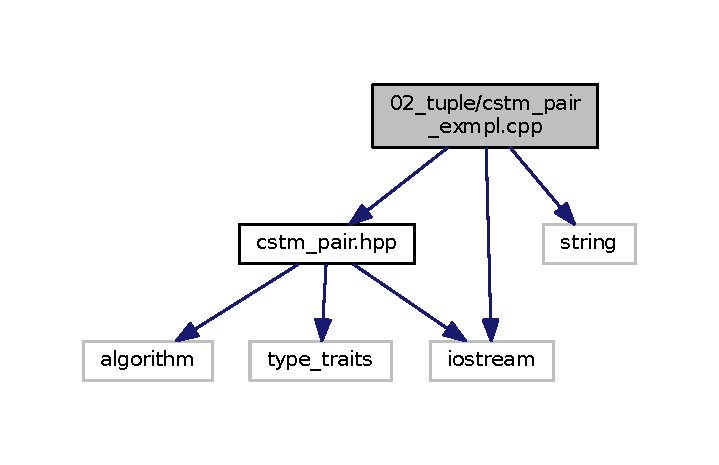
\includegraphics[width=345pt]{cstm__pair__exmpl_8cpp__incl}
\end{center}
\end{figure}
\subsection*{Functions}
\begin{DoxyCompactItemize}
\item 
auto \hyperlink{cstm__pair__exmpl_8cpp_ae67256938aa05b1d4bb49651db1d7acd}{get\+Person} ()
\item 
int \hyperlink{cstm__pair__exmpl_8cpp_a0ddf1224851353fc92bfbff6f499fa97}{main} (int argc, char $\ast$argv\mbox{[}$\,$\mbox{]})
\end{DoxyCompactItemize}


\subsection{Function Documentation}
\index{cstm\+\_\+pair\+\_\+exmpl.\+cpp@{cstm\+\_\+pair\+\_\+exmpl.\+cpp}!get\+Person@{get\+Person}}
\index{get\+Person@{get\+Person}!cstm\+\_\+pair\+\_\+exmpl.\+cpp@{cstm\+\_\+pair\+\_\+exmpl.\+cpp}}
\subsubsection[{\texorpdfstring{get\+Person()}{getPerson()}}]{\setlength{\rightskip}{0pt plus 5cm}auto get\+Person (
\begin{DoxyParamCaption}
{}
\end{DoxyParamCaption}
)}\hypertarget{cstm__pair__exmpl_8cpp_ae67256938aa05b1d4bb49651db1d7acd}{}\label{cstm__pair__exmpl_8cpp_ae67256938aa05b1d4bb49651db1d7acd}
\index{cstm\+\_\+pair\+\_\+exmpl.\+cpp@{cstm\+\_\+pair\+\_\+exmpl.\+cpp}!main@{main}}
\index{main@{main}!cstm\+\_\+pair\+\_\+exmpl.\+cpp@{cstm\+\_\+pair\+\_\+exmpl.\+cpp}}
\subsubsection[{\texorpdfstring{main(int argc, char $\ast$argv[])}{main(int argc, char *argv[])}}]{\setlength{\rightskip}{0pt plus 5cm}int main (
\begin{DoxyParamCaption}
\item[{int}]{argc, }
\item[{char $\ast$}]{argv\mbox{[}$\,$\mbox{]}}
\end{DoxyParamCaption}
)}\hypertarget{cstm__pair__exmpl_8cpp_a0ddf1224851353fc92bfbff6f499fa97}{}\label{cstm__pair__exmpl_8cpp_a0ddf1224851353fc92bfbff6f499fa97}

\hypertarget{cstm__pair__exmpl__2_8cpp}{}\section{02\+\_\+tuple/cstm\+\_\+pair\+\_\+exmpl\+\_\+2.cpp File Reference}
\label{cstm__pair__exmpl__2_8cpp}\index{02\+\_\+tuple/cstm\+\_\+pair\+\_\+exmpl\+\_\+2.\+cpp@{02\+\_\+tuple/cstm\+\_\+pair\+\_\+exmpl\+\_\+2.\+cpp}}
{\ttfamily \#include \char`\"{}cstm\+\_\+pair\+\_\+2.\+hpp\char`\"{}}\\*
{\ttfamily \#include $<$iostream$>$}\\*
{\ttfamily \#include $<$string$>$}\\*
Include dependency graph for cstm\+\_\+pair\+\_\+exmpl\+\_\+2.\+cpp\+:
\nopagebreak
\begin{figure}[H]
\begin{center}
\leavevmode
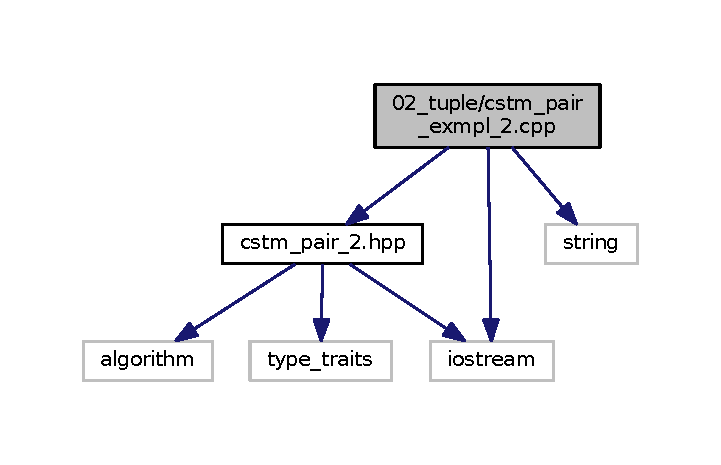
\includegraphics[width=346pt]{cstm__pair__exmpl__2_8cpp__incl}
\end{center}
\end{figure}
\subsection*{Functions}
\begin{DoxyCompactItemize}
\item 
auto \hyperlink{cstm__pair__exmpl__2_8cpp_ae67256938aa05b1d4bb49651db1d7acd}{get\+Person} ()
\item 
int \hyperlink{cstm__pair__exmpl__2_8cpp_a0ddf1224851353fc92bfbff6f499fa97}{main} (int argc, char $\ast$argv\mbox{[}$\,$\mbox{]})
\end{DoxyCompactItemize}


\subsection{Function Documentation}
\index{cstm\+\_\+pair\+\_\+exmpl\+\_\+2.\+cpp@{cstm\+\_\+pair\+\_\+exmpl\+\_\+2.\+cpp}!get\+Person@{get\+Person}}
\index{get\+Person@{get\+Person}!cstm\+\_\+pair\+\_\+exmpl\+\_\+2.\+cpp@{cstm\+\_\+pair\+\_\+exmpl\+\_\+2.\+cpp}}
\subsubsection[{\texorpdfstring{get\+Person()}{getPerson()}}]{\setlength{\rightskip}{0pt plus 5cm}auto get\+Person (
\begin{DoxyParamCaption}
{}
\end{DoxyParamCaption}
)}\hypertarget{cstm__pair__exmpl__2_8cpp_ae67256938aa05b1d4bb49651db1d7acd}{}\label{cstm__pair__exmpl__2_8cpp_ae67256938aa05b1d4bb49651db1d7acd}
\index{cstm\+\_\+pair\+\_\+exmpl\+\_\+2.\+cpp@{cstm\+\_\+pair\+\_\+exmpl\+\_\+2.\+cpp}!main@{main}}
\index{main@{main}!cstm\+\_\+pair\+\_\+exmpl\+\_\+2.\+cpp@{cstm\+\_\+pair\+\_\+exmpl\+\_\+2.\+cpp}}
\subsubsection[{\texorpdfstring{main(int argc, char $\ast$argv[])}{main(int argc, char *argv[])}}]{\setlength{\rightskip}{0pt plus 5cm}int main (
\begin{DoxyParamCaption}
\item[{int}]{argc, }
\item[{char $\ast$}]{argv\mbox{[}$\,$\mbox{]}}
\end{DoxyParamCaption}
)}\hypertarget{cstm__pair__exmpl__2_8cpp_a0ddf1224851353fc92bfbff6f499fa97}{}\label{cstm__pair__exmpl__2_8cpp_a0ddf1224851353fc92bfbff6f499fa97}

\hypertarget{cstm__tuple_8hpp}{}\section{02\+\_\+tuple/cstm\+\_\+tuple.hpp File Reference}
\label{cstm__tuple_8hpp}\index{02\+\_\+tuple/cstm\+\_\+tuple.\+hpp@{02\+\_\+tuple/cstm\+\_\+tuple.\+hpp}}
{\ttfamily \#include $<$iostream$>$}\\*
{\ttfamily \#include $<$string$>$}\\*
{\ttfamily \#include $<$cassert$>$}\\*
{\ttfamily \#include $<$cstdint$>$}\\*
{\ttfamily \#include $<$typeinfo$>$}\\*
{\ttfamily \#include $<$cstddef$>$}\\*
Include dependency graph for cstm\+\_\+tuple.\+hpp\+:
\nopagebreak
\begin{figure}[H]
\begin{center}
\leavevmode
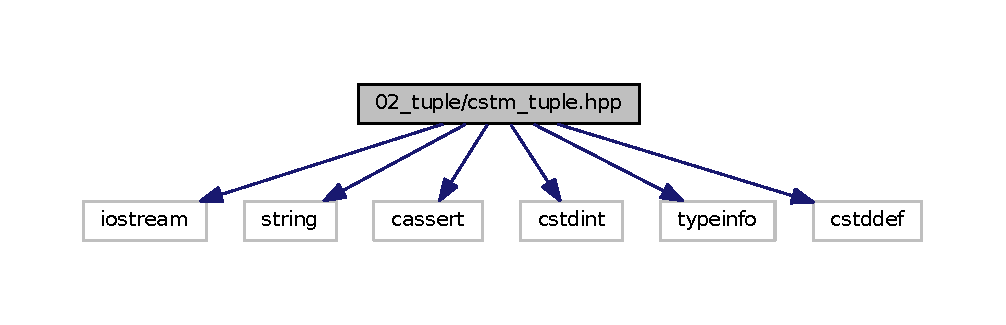
\includegraphics[width=350pt]{cstm__tuple_8hpp__incl}
\end{center}
\end{figure}
This graph shows which files directly or indirectly include this file\+:
\nopagebreak
\begin{figure}[H]
\begin{center}
\leavevmode
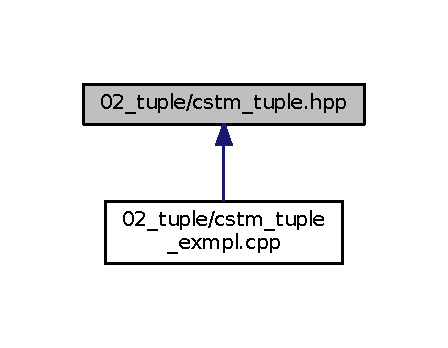
\includegraphics[width=215pt]{cstm__tuple_8hpp__dep__incl}
\end{center}
\end{figure}
\subsection*{Classes}
\begin{DoxyCompactItemize}
\item 
struct \hyperlink{structcustom__tuple}{custom\+\_\+tuple$<$ Types $>$}
\item 
struct \hyperlink{structcustom__tuple_3_01T_00_01Types_8_8_8_01_4}{custom\+\_\+tuple$<$ T, Types... $>$}
\item 
struct \hyperlink{structelem__type__holder}{elem\+\_\+type\+\_\+holder$<$ size\+\_\+t, typename $>$}
\item 
struct \hyperlink{structelem__type__holder_3_010_00_01custom__tuple_3_01T_00_01Ts_8_8_8_01_4_01_4}{elem\+\_\+type\+\_\+holder$<$ 0, custom\+\_\+tuple$<$ T, Ts... $>$ $>$}
\item 
struct \hyperlink{structelem__type__holder_3_01k_00_01custom__tuple_3_01T_00_01Ts_8_8_8_01_4_01_4}{elem\+\_\+type\+\_\+holder$<$ k, custom\+\_\+tuple$<$ T, Ts... $>$ $>$}
\end{DoxyCompactItemize}
\subsection*{Functions}
\begin{DoxyCompactItemize}
\item 
{\footnotesize template$<$size\+\_\+t k, typename... Types$>$ }\\std\+::enable\+\_\+if\+\_\+t$<$ k==0, typename \hyperlink{structelem__type__holder}{elem\+\_\+type\+\_\+holder}$<$ 0, \hyperlink{structcustom__tuple}{custom\+\_\+tuple}$<$ Types... $>$ $>$\+::type \& $>$ \hyperlink{cstm__tuple_8hpp_ace875a167aa434ff372f40dd99ac0694}{get} (\hyperlink{structcustom__tuple}{custom\+\_\+tuple}$<$ Types... $>$ \&ct)
\item 
{\footnotesize template$<$size\+\_\+t k, typename T , typename... Types$>$ }\\std\+::enable\+\_\+if\+\_\+t$<$ k!=0, typename \hyperlink{structelem__type__holder}{elem\+\_\+type\+\_\+holder}$<$ k, \hyperlink{structcustom__tuple}{custom\+\_\+tuple}$<$ T, Types... $>$ $>$\+::type \& $>$ \hyperlink{cstm__tuple_8hpp_aba451cbb702ef2407f373818725abcad}{get} (\hyperlink{structcustom__tuple}{custom\+\_\+tuple}$<$ T, Types... $>$ \&ct)
\item 
{\footnotesize template$<$typename... Types$>$ }\\auto \hyperlink{cstm__tuple_8hpp_aed4eda5a742f86f514dac3e022f8429d}{make\+\_\+custom\+\_\+tuple} (Types...\+args)
\item 
{\footnotesize template$<$typename... Types$>$ }\\auto \hyperlink{cstm__tuple_8hpp_a2afbfdeedd1bf8afc04f7849f4648f6c}{custom\+\_\+tie} (Types \&...args) noexcept
\end{DoxyCompactItemize}


\subsection{Function Documentation}
\index{cstm\+\_\+tuple.\+hpp@{cstm\+\_\+tuple.\+hpp}!custom\+\_\+tie@{custom\+\_\+tie}}
\index{custom\+\_\+tie@{custom\+\_\+tie}!cstm\+\_\+tuple.\+hpp@{cstm\+\_\+tuple.\+hpp}}
\subsubsection[{\texorpdfstring{custom\+\_\+tie(\+Types \&...\+args) noexcept}{custom_tie(Types &...args) noexcept}}]{\setlength{\rightskip}{0pt plus 5cm}template$<$typename... Types$>$ auto custom\+\_\+tie (
\begin{DoxyParamCaption}
\item[{Types \&...}]{args}
\end{DoxyParamCaption}
)\hspace{0.3cm}{\ttfamily [noexcept]}}\hypertarget{cstm__tuple_8hpp_a2afbfdeedd1bf8afc04f7849f4648f6c}{}\label{cstm__tuple_8hpp_a2afbfdeedd1bf8afc04f7849f4648f6c}
\index{cstm\+\_\+tuple.\+hpp@{cstm\+\_\+tuple.\+hpp}!get@{get}}
\index{get@{get}!cstm\+\_\+tuple.\+hpp@{cstm\+\_\+tuple.\+hpp}}
\subsubsection[{\texorpdfstring{get(custom\+\_\+tuple$<$ Types... $>$ \&ct)}{get(custom_tuple< Types... > &ct)}}]{\setlength{\rightskip}{0pt plus 5cm}template$<$size\+\_\+t k, typename... Types$>$ std\+::enable\+\_\+if\+\_\+t$<$k == 0, typename {\bf elem\+\_\+type\+\_\+holder}$<$0, {\bf custom\+\_\+tuple}$<$Types ... $>$ $>$\+::type\& $>$ get (
\begin{DoxyParamCaption}
\item[{{\bf custom\+\_\+tuple}$<$ Types... $>$ \&}]{ct}
\end{DoxyParamCaption}
)}\hypertarget{cstm__tuple_8hpp_ace875a167aa434ff372f40dd99ac0694}{}\label{cstm__tuple_8hpp_ace875a167aa434ff372f40dd99ac0694}
\index{cstm\+\_\+tuple.\+hpp@{cstm\+\_\+tuple.\+hpp}!get@{get}}
\index{get@{get}!cstm\+\_\+tuple.\+hpp@{cstm\+\_\+tuple.\+hpp}}
\subsubsection[{\texorpdfstring{get(custom\+\_\+tuple$<$ T, Types... $>$ \&ct)}{get(custom_tuple< T, Types... > &ct)}}]{\setlength{\rightskip}{0pt plus 5cm}template$<$size\+\_\+t k, typename T , typename... Types$>$ std\+::enable\+\_\+if\+\_\+t$<$k != 0, typename {\bf elem\+\_\+type\+\_\+holder}$<$k, {\bf custom\+\_\+tuple}$<$T, Types ... $>$ $>$\+::type \& $>$ get (
\begin{DoxyParamCaption}
\item[{{\bf custom\+\_\+tuple}$<$ T, Types... $>$ \&}]{ct}
\end{DoxyParamCaption}
)}\hypertarget{cstm__tuple_8hpp_aba451cbb702ef2407f373818725abcad}{}\label{cstm__tuple_8hpp_aba451cbb702ef2407f373818725abcad}
\index{cstm\+\_\+tuple.\+hpp@{cstm\+\_\+tuple.\+hpp}!make\+\_\+custom\+\_\+tuple@{make\+\_\+custom\+\_\+tuple}}
\index{make\+\_\+custom\+\_\+tuple@{make\+\_\+custom\+\_\+tuple}!cstm\+\_\+tuple.\+hpp@{cstm\+\_\+tuple.\+hpp}}
\subsubsection[{\texorpdfstring{make\+\_\+custom\+\_\+tuple(\+Types...\+args)}{make_custom_tuple(Types...args)}}]{\setlength{\rightskip}{0pt plus 5cm}template$<$typename... Types$>$ auto make\+\_\+custom\+\_\+tuple (
\begin{DoxyParamCaption}
\item[{Types...}]{args}
\end{DoxyParamCaption}
)}\hypertarget{cstm__tuple_8hpp_aed4eda5a742f86f514dac3e022f8429d}{}\label{cstm__tuple_8hpp_aed4eda5a742f86f514dac3e022f8429d}

\hypertarget{cstm__tuple__exmpl_8cpp}{}\section{02\+\_\+tuple/cstm\+\_\+tuple\+\_\+exmpl.cpp File Reference}
\label{cstm__tuple__exmpl_8cpp}\index{02\+\_\+tuple/cstm\+\_\+tuple\+\_\+exmpl.\+cpp@{02\+\_\+tuple/cstm\+\_\+tuple\+\_\+exmpl.\+cpp}}
{\ttfamily \#include \char`\"{}cstm\+\_\+tuple.\+hpp\char`\"{}}\\*
{\ttfamily \#include $<$string$>$}\\*
Include dependency graph for cstm\+\_\+tuple\+\_\+exmpl.\+cpp\+:
\nopagebreak
\begin{figure}[H]
\begin{center}
\leavevmode
\includegraphics[width=350pt]{cstm__tuple__exmpl_8cpp__incl}
\end{center}
\end{figure}
\subsection*{Functions}
\begin{DoxyCompactItemize}
\item 
auto \hyperlink{cstm__tuple__exmpl_8cpp_ae67256938aa05b1d4bb49651db1d7acd}{get\+Person} ()
\item 
auto \hyperlink{cstm__tuple__exmpl_8cpp_a290da9ec9671d3f6d8be6f84c862678e}{get\+Person1} ()
\item 
int \hyperlink{cstm__tuple__exmpl_8cpp_a3c04138a5bfe5d72780bb7e82a18e627}{main} (int argc, char $\ast$$\ast$argv)
\end{DoxyCompactItemize}


\subsection{Function Documentation}
\index{cstm\+\_\+tuple\+\_\+exmpl.\+cpp@{cstm\+\_\+tuple\+\_\+exmpl.\+cpp}!get\+Person@{get\+Person}}
\index{get\+Person@{get\+Person}!cstm\+\_\+tuple\+\_\+exmpl.\+cpp@{cstm\+\_\+tuple\+\_\+exmpl.\+cpp}}
\subsubsection[{\texorpdfstring{get\+Person()}{getPerson()}}]{\setlength{\rightskip}{0pt plus 5cm}auto get\+Person (
\begin{DoxyParamCaption}
{}
\end{DoxyParamCaption}
)}\hypertarget{cstm__tuple__exmpl_8cpp_ae67256938aa05b1d4bb49651db1d7acd}{}\label{cstm__tuple__exmpl_8cpp_ae67256938aa05b1d4bb49651db1d7acd}
\index{cstm\+\_\+tuple\+\_\+exmpl.\+cpp@{cstm\+\_\+tuple\+\_\+exmpl.\+cpp}!get\+Person1@{get\+Person1}}
\index{get\+Person1@{get\+Person1}!cstm\+\_\+tuple\+\_\+exmpl.\+cpp@{cstm\+\_\+tuple\+\_\+exmpl.\+cpp}}
\subsubsection[{\texorpdfstring{get\+Person1()}{getPerson1()}}]{\setlength{\rightskip}{0pt plus 5cm}auto get\+Person1 (
\begin{DoxyParamCaption}
{}
\end{DoxyParamCaption}
)}\hypertarget{cstm__tuple__exmpl_8cpp_a290da9ec9671d3f6d8be6f84c862678e}{}\label{cstm__tuple__exmpl_8cpp_a290da9ec9671d3f6d8be6f84c862678e}
\index{cstm\+\_\+tuple\+\_\+exmpl.\+cpp@{cstm\+\_\+tuple\+\_\+exmpl.\+cpp}!main@{main}}
\index{main@{main}!cstm\+\_\+tuple\+\_\+exmpl.\+cpp@{cstm\+\_\+tuple\+\_\+exmpl.\+cpp}}
\subsubsection[{\texorpdfstring{main(int argc, char $\ast$$\ast$argv)}{main(int argc, char **argv)}}]{\setlength{\rightskip}{0pt plus 5cm}int main (
\begin{DoxyParamCaption}
\item[{int}]{argc, }
\item[{char $\ast$$\ast$}]{argv}
\end{DoxyParamCaption}
)}\hypertarget{cstm__tuple__exmpl_8cpp_a3c04138a5bfe5d72780bb7e82a18e627}{}\label{cstm__tuple__exmpl_8cpp_a3c04138a5bfe5d72780bb7e82a18e627}

\hypertarget{custom__container_8hpp}{}\section{03\+\_\+allocator/custom\+\_\+container.hpp File Reference}
\label{custom__container_8hpp}\index{03\+\_\+allocator/custom\+\_\+container.\+hpp@{03\+\_\+allocator/custom\+\_\+container.\+hpp}}
{\ttfamily \#include $<$memory$>$}\\*
{\ttfamily \#include $<$cstddef$>$}\\*
{\ttfamily \#include $<$iostream$>$}\\*
Include dependency graph for custom\+\_\+container.\+hpp\+:
\nopagebreak
\begin{figure}[H]
\begin{center}
\leavevmode
\includegraphics[width=285pt]{custom__container_8hpp__incl}
\end{center}
\end{figure}
This graph shows which files directly or indirectly include this file\+:
\nopagebreak
\begin{figure}[H]
\begin{center}
\leavevmode
\includegraphics[width=268pt]{custom__container_8hpp__dep__incl}
\end{center}
\end{figure}
\subsection*{Classes}
\begin{DoxyCompactItemize}
\item 
class \hyperlink{classCustomContainer}{Custom\+Container$<$ T, allocator\+\_\+type $>$}
\end{DoxyCompactItemize}

\hypertarget{fixed__sz__allocator_8hpp}{}\section{03\+\_\+allocator/fixed\+\_\+sz\+\_\+allocator.hpp File Reference}
\label{fixed__sz__allocator_8hpp}\index{03\+\_\+allocator/fixed\+\_\+sz\+\_\+allocator.\+hpp@{03\+\_\+allocator/fixed\+\_\+sz\+\_\+allocator.\+hpp}}
{\ttfamily \#include $<$array$>$}\\*
{\ttfamily \#include $<$string$>$}\\*
{\ttfamily \#include $<$exception$>$}\\*
{\ttfamily \#include $<$iostream$>$}\\*
Include dependency graph for fixed\+\_\+sz\+\_\+allocator.\+hpp\+:
\nopagebreak
\begin{figure}[H]
\begin{center}
\leavevmode
\includegraphics[width=342pt]{fixed__sz__allocator_8hpp__incl}
\end{center}
\end{figure}
This graph shows which files directly or indirectly include this file\+:
\nopagebreak
\begin{figure}[H]
\begin{center}
\leavevmode
\includegraphics[width=350pt]{fixed__sz__allocator_8hpp__dep__incl}
\end{center}
\end{figure}
\subsection*{Classes}
\begin{DoxyCompactItemize}
\item 
class \hyperlink{classreserve__allocator}{reserve\+\_\+allocator$<$ T, n $>$}
\item 
struct \hyperlink{structreserve__allocator_1_1rebind}{reserve\+\_\+allocator$<$ T, n $>$\+::rebind$<$ U $>$}
\end{DoxyCompactItemize}

\hypertarget{flexible__allocator_8hpp}{}\section{03\+\_\+allocator/flexible\+\_\+allocator.hpp File Reference}
\label{flexible__allocator_8hpp}\index{03\+\_\+allocator/flexible\+\_\+allocator.\+hpp@{03\+\_\+allocator/flexible\+\_\+allocator.\+hpp}}
{\ttfamily \#include $<$cstddef$>$}\\*
{\ttfamily \#include $<$iostream$>$}\\*
{\ttfamily \#include $<$vector$>$}\\*
{\ttfamily \#include $<$memory$>$}\\*
{\ttfamily \#include $<$list$>$}\\*
Include dependency graph for flexible\+\_\+allocator.\+hpp\+:
\nopagebreak
\begin{figure}[H]
\begin{center}
\leavevmode
\includegraphics[width=350pt]{flexible__allocator_8hpp__incl}
\end{center}
\end{figure}
This graph shows which files directly or indirectly include this file\+:
\nopagebreak
\begin{figure}[H]
\begin{center}
\leavevmode
\includegraphics[width=248pt]{flexible__allocator_8hpp__dep__incl}
\end{center}
\end{figure}
\subsection*{Classes}
\begin{DoxyCompactItemize}
\item 
class \hyperlink{classcontigious__block}{contigious\+\_\+block$<$ T $>$}
\item 
class \hyperlink{classelementwise__block__allocator}{elementwise\+\_\+block\+\_\+allocator$<$ T $>$}
\end{DoxyCompactItemize}

\hypertarget{main__allocator_8cpp}{}\section{03\+\_\+allocator/main\+\_\+allocator.cpp File Reference}
\label{main__allocator_8cpp}\index{03\+\_\+allocator/main\+\_\+allocator.\+cpp@{03\+\_\+allocator/main\+\_\+allocator.\+cpp}}
{\ttfamily \#include \char`\"{}flexible\+\_\+allocator.\+hpp\char`\"{}}\\*
{\ttfamily \#include \char`\"{}fixed\+\_\+sz\+\_\+allocator.\+hpp\char`\"{}}\\*
{\ttfamily \#include \char`\"{}custom\+\_\+container.\+hpp\char`\"{}}\\*
{\ttfamily \#include \char`\"{}reserved\+\_\+container.\+hpp\char`\"{}}\\*
{\ttfamily \#include $<$iostream$>$}\\*
{\ttfamily \#include $<$map$>$}\\*
Include dependency graph for main\+\_\+allocator.\+cpp\+:
\nopagebreak
\begin{figure}[H]
\begin{center}
\leavevmode
\includegraphics[width=350pt]{main__allocator_8cpp__incl}
\end{center}
\end{figure}
\subsection*{Functions}
\begin{DoxyCompactItemize}
\item 
int \hyperlink{main__allocator_8cpp_a0ddf1224851353fc92bfbff6f499fa97}{main} (int argc, char $\ast$argv\mbox{[}$\,$\mbox{]})
\end{DoxyCompactItemize}


\subsection{Function Documentation}
\index{main\+\_\+allocator.\+cpp@{main\+\_\+allocator.\+cpp}!main@{main}}
\index{main@{main}!main\+\_\+allocator.\+cpp@{main\+\_\+allocator.\+cpp}}
\subsubsection[{\texorpdfstring{main(int argc, char $\ast$argv[])}{main(int argc, char *argv[])}}]{\setlength{\rightskip}{0pt plus 5cm}int main (
\begin{DoxyParamCaption}
\item[{int}]{argc, }
\item[{char $\ast$}]{argv\mbox{[}$\,$\mbox{]}}
\end{DoxyParamCaption}
)}\hypertarget{main__allocator_8cpp_a0ddf1224851353fc92bfbff6f499fa97}{}\label{main__allocator_8cpp_a0ddf1224851353fc92bfbff6f499fa97}

\hypertarget{reserved__container_8hpp}{}\section{03\+\_\+allocator/reserved\+\_\+container.hpp File Reference}
\label{reserved__container_8hpp}\index{03\+\_\+allocator/reserved\+\_\+container.\+hpp@{03\+\_\+allocator/reserved\+\_\+container.\+hpp}}
{\ttfamily \#include \char`\"{}custom\+\_\+container.\+hpp\char`\"{}}\\*
Include dependency graph for reserved\+\_\+container.\+hpp\+:
\nopagebreak
\begin{figure}[H]
\begin{center}
\leavevmode
\includegraphics[width=285pt]{reserved__container_8hpp__incl}
\end{center}
\end{figure}
This graph shows which files directly or indirectly include this file\+:
\nopagebreak
\begin{figure}[H]
\begin{center}
\leavevmode
\includegraphics[width=248pt]{reserved__container_8hpp__dep__incl}
\end{center}
\end{figure}
\subsection*{Classes}
\begin{DoxyCompactItemize}
\item 
class \hyperlink{classCustomContainer_3_01T_00_01reserve__allocator_3_01T_00_01n_01_4_01_4}{Custom\+Container$<$ T, reserve\+\_\+allocator$<$ T, n $>$ $>$}
\end{DoxyCompactItemize}
\subsection*{Typedefs}
\begin{DoxyCompactItemize}
\item 
{\footnotesize template$<$typename T , size\+\_\+t n$>$ }\\using \hyperlink{reserved__container_8hpp_a645c90241dfa63f57e4e174b957f076a}{Reserved\+Container} = \hyperlink{classCustomContainer}{Custom\+Container}$<$ T, \hyperlink{classreserve__allocator}{reserve\+\_\+allocator}$<$ T, n $>$$>$
\end{DoxyCompactItemize}


\subsection{Typedef Documentation}
\index{reserved\+\_\+container.\+hpp@{reserved\+\_\+container.\+hpp}!Reserved\+Container@{Reserved\+Container}}
\index{Reserved\+Container@{Reserved\+Container}!reserved\+\_\+container.\+hpp@{reserved\+\_\+container.\+hpp}}
\subsubsection[{\texorpdfstring{Reserved\+Container}{ReservedContainer}}]{\setlength{\rightskip}{0pt plus 5cm}template$<$typename T , size\+\_\+t n$>$ using {\bf Reserved\+Container} =  {\bf Custom\+Container}$<$T, {\bf reserve\+\_\+allocator}$<$T, n$>$$>$}\hypertarget{reserved__container_8hpp_a645c90241dfa63f57e4e174b957f076a}{}\label{reserved__container_8hpp_a645c90241dfa63f57e4e174b957f076a}

\hypertarget{test__allocator_8cpp}{}\section{03\+\_\+allocator/test\+\_\+allocator.cpp File Reference}
\label{test__allocator_8cpp}\index{03\+\_\+allocator/test\+\_\+allocator.\+cpp@{03\+\_\+allocator/test\+\_\+allocator.\+cpp}}
{\ttfamily \#include \char`\"{}fixed\+\_\+sz\+\_\+allocator.\+hpp\char`\"{}}\\*
{\ttfamily \#include $<$gtest/gtest.\+h$>$}\\*
{\ttfamily \#include $<$iostream$>$}\\*
Include dependency graph for test\+\_\+allocator.\+cpp\+:
\nopagebreak
\begin{figure}[H]
\begin{center}
\leavevmode
\includegraphics[width=350pt]{test__allocator_8cpp__incl}
\end{center}
\end{figure}
\subsection*{Functions}
\begin{DoxyCompactItemize}
\item 
\hyperlink{test__allocator_8cpp_a9a03f3ab02a05326d0e17811607fa4d4}{T\+E\+ST} (allocator, base\+\_\+operations)
\item 
\hyperlink{test__allocator_8cpp_a43054c06095011c4e988b8c2e744ff74}{T\+E\+ST} (allocator, insert\+\_\+operations)
\item 
\hyperlink{test__allocator_8cpp_aa3413cdc9a6ad9e8a89542a706e87e3d}{T\+E\+ST} (allocator, remove\+\_\+operations)
\item 
int \hyperlink{test__allocator_8cpp_a0ddf1224851353fc92bfbff6f499fa97}{main} (int argc, char $\ast$argv\mbox{[}$\,$\mbox{]})
\end{DoxyCompactItemize}


\subsection{Function Documentation}
\index{test\+\_\+allocator.\+cpp@{test\+\_\+allocator.\+cpp}!main@{main}}
\index{main@{main}!test\+\_\+allocator.\+cpp@{test\+\_\+allocator.\+cpp}}
\subsubsection[{\texorpdfstring{main(int argc, char $\ast$argv[])}{main(int argc, char *argv[])}}]{\setlength{\rightskip}{0pt plus 5cm}int main (
\begin{DoxyParamCaption}
\item[{int}]{argc, }
\item[{char $\ast$}]{argv\mbox{[}$\,$\mbox{]}}
\end{DoxyParamCaption}
)}\hypertarget{test__allocator_8cpp_a0ddf1224851353fc92bfbff6f499fa97}{}\label{test__allocator_8cpp_a0ddf1224851353fc92bfbff6f499fa97}
\index{test\+\_\+allocator.\+cpp@{test\+\_\+allocator.\+cpp}!T\+E\+ST@{T\+E\+ST}}
\index{T\+E\+ST@{T\+E\+ST}!test\+\_\+allocator.\+cpp@{test\+\_\+allocator.\+cpp}}
\subsubsection[{\texorpdfstring{T\+E\+S\+T(allocator, base\+\_\+operations)}{TEST(allocator, base_operations)}}]{\setlength{\rightskip}{0pt plus 5cm}T\+E\+ST (
\begin{DoxyParamCaption}
\item[{allocator}]{, }
\item[{base\+\_\+operations}]{}
\end{DoxyParamCaption}
)}\hypertarget{test__allocator_8cpp_a9a03f3ab02a05326d0e17811607fa4d4}{}\label{test__allocator_8cpp_a9a03f3ab02a05326d0e17811607fa4d4}
\index{test\+\_\+allocator.\+cpp@{test\+\_\+allocator.\+cpp}!T\+E\+ST@{T\+E\+ST}}
\index{T\+E\+ST@{T\+E\+ST}!test\+\_\+allocator.\+cpp@{test\+\_\+allocator.\+cpp}}
\subsubsection[{\texorpdfstring{T\+E\+S\+T(allocator, insert\+\_\+operations)}{TEST(allocator, insert_operations)}}]{\setlength{\rightskip}{0pt plus 5cm}T\+E\+ST (
\begin{DoxyParamCaption}
\item[{allocator}]{, }
\item[{insert\+\_\+operations}]{}
\end{DoxyParamCaption}
)}\hypertarget{test__allocator_8cpp_a43054c06095011c4e988b8c2e744ff74}{}\label{test__allocator_8cpp_a43054c06095011c4e988b8c2e744ff74}
\index{test\+\_\+allocator.\+cpp@{test\+\_\+allocator.\+cpp}!T\+E\+ST@{T\+E\+ST}}
\index{T\+E\+ST@{T\+E\+ST}!test\+\_\+allocator.\+cpp@{test\+\_\+allocator.\+cpp}}
\subsubsection[{\texorpdfstring{T\+E\+S\+T(allocator, remove\+\_\+operations)}{TEST(allocator, remove_operations)}}]{\setlength{\rightskip}{0pt plus 5cm}T\+E\+ST (
\begin{DoxyParamCaption}
\item[{allocator}]{, }
\item[{remove\+\_\+operations}]{}
\end{DoxyParamCaption}
)}\hypertarget{test__allocator_8cpp_aa3413cdc9a6ad9e8a89542a706e87e3d}{}\label{test__allocator_8cpp_aa3413cdc9a6ad9e8a89542a706e87e3d}

\hypertarget{test__out_8cpp}{}\section{03\+\_\+ranges/test\+\_\+out.cpp File Reference}
\label{test__out_8cpp}\index{03\+\_\+ranges/test\+\_\+out.\+cpp@{03\+\_\+ranges/test\+\_\+out.\+cpp}}
{\ttfamily \#include \char`\"{}ip\+\_\+processor.\+h\char`\"{}}\\*
{\ttfamily \#include $<$gtest/gtest.\+h$>$}\\*
{\ttfamily \#include $<$iostream$>$}\\*
{\ttfamily \#include $<$fstream$>$}\\*
{\ttfamily \#include $<$memory$>$}\\*
{\ttfamily \#include $<$cstdlib$>$}\\*
{\ttfamily \#include $<$cstdio$>$}\\*
Include dependency graph for test\+\_\+out.\+cpp\+:
\nopagebreak
\begin{figure}[H]
\begin{center}
\leavevmode
\includegraphics[width=350pt]{test__out_8cpp__incl}
\end{center}
\end{figure}
\subsection*{Functions}
\begin{DoxyCompactItemize}
\item 
\hyperlink{test__out_8cpp_a8ec24fc6035afdb0d266b9357c1cab9a}{T\+E\+ST} (test\+\_\+all\+\_\+results, ip)
\item 
int \hyperlink{test__out_8cpp_a0ddf1224851353fc92bfbff6f499fa97}{main} (int argc, char $\ast$argv\mbox{[}$\,$\mbox{]})
\end{DoxyCompactItemize}
\subsection*{Variables}
\begin{DoxyCompactItemize}
\item 
char $\ast$$\ast$ \hyperlink{test__out_8cpp_a05f58fe144fe2e6f1308c688cee7321c}{my\+\_\+argv}
\end{DoxyCompactItemize}


\subsection{Function Documentation}
\index{test\+\_\+out.\+cpp@{test\+\_\+out.\+cpp}!main@{main}}
\index{main@{main}!test\+\_\+out.\+cpp@{test\+\_\+out.\+cpp}}
\subsubsection[{\texorpdfstring{main(int argc, char $\ast$argv[])}{main(int argc, char *argv[])}}]{\setlength{\rightskip}{0pt plus 5cm}int main (
\begin{DoxyParamCaption}
\item[{int}]{argc, }
\item[{char $\ast$}]{argv\mbox{[}$\,$\mbox{]}}
\end{DoxyParamCaption}
)}\hypertarget{test__out_8cpp_a0ddf1224851353fc92bfbff6f499fa97}{}\label{test__out_8cpp_a0ddf1224851353fc92bfbff6f499fa97}
\index{test\+\_\+out.\+cpp@{test\+\_\+out.\+cpp}!T\+E\+ST@{T\+E\+ST}}
\index{T\+E\+ST@{T\+E\+ST}!test\+\_\+out.\+cpp@{test\+\_\+out.\+cpp}}
\subsubsection[{\texorpdfstring{T\+E\+S\+T(test\+\_\+all\+\_\+results, ip)}{TEST(test_all_results, ip)}}]{\setlength{\rightskip}{0pt plus 5cm}T\+E\+ST (
\begin{DoxyParamCaption}
\item[{test\+\_\+all\+\_\+results}]{, }
\item[{ip}]{}
\end{DoxyParamCaption}
)}\hypertarget{test__out_8cpp_a8ec24fc6035afdb0d266b9357c1cab9a}{}\label{test__out_8cpp_a8ec24fc6035afdb0d266b9357c1cab9a}


\subsection{Variable Documentation}
\index{test\+\_\+out.\+cpp@{test\+\_\+out.\+cpp}!my\+\_\+argv@{my\+\_\+argv}}
\index{my\+\_\+argv@{my\+\_\+argv}!test\+\_\+out.\+cpp@{test\+\_\+out.\+cpp}}
\subsubsection[{\texorpdfstring{my\+\_\+argv}{my_argv}}]{\setlength{\rightskip}{0pt plus 5cm}char$\ast$$\ast$ my\+\_\+argv}\hypertarget{test__out_8cpp_a05f58fe144fe2e6f1308c688cee7321c}{}\label{test__out_8cpp_a05f58fe144fe2e6f1308c688cee7321c}

\hypertarget{print__ip__04_8hpp}{}\section{04\+\_\+sfinae/print\+\_\+ip\+\_\+04.hpp File Reference}
\label{print__ip__04_8hpp}\index{04\+\_\+sfinae/print\+\_\+ip\+\_\+04.\+hpp@{04\+\_\+sfinae/print\+\_\+ip\+\_\+04.\+hpp}}
{\ttfamily \#include $<$type\+\_\+traits$>$}\\*
{\ttfamily \#include $<$iostream$>$}\\*
{\ttfamily \#include $<$string$>$}\\*
{\ttfamily \#include $<$vector$>$}\\*
{\ttfamily \#include $<$list$>$}\\*
{\ttfamily \#include $<$tuple$>$}\\*
{\ttfamily \#include $<$bitset$>$}\\*
{\ttfamily \#include $<$cstdint$>$}\\*
Include dependency graph for print\+\_\+ip\+\_\+04.\+hpp\+:
\nopagebreak
\begin{figure}[H]
\begin{center}
\leavevmode
\includegraphics[width=350pt]{print__ip__04_8hpp__incl}
\end{center}
\end{figure}
This graph shows which files directly or indirectly include this file\+:
\nopagebreak
\begin{figure}[H]
\begin{center}
\leavevmode
\includegraphics[width=320pt]{print__ip__04_8hpp__dep__incl}
\end{center}
\end{figure}
\subsection*{Classes}
\begin{DoxyCompactItemize}
\item 
struct \hyperlink{structis__std__string}{is\+\_\+std\+\_\+string$<$ T $>$}
\item 
struct \hyperlink{structis__std__string_3_01std_1_1string_01_4}{is\+\_\+std\+\_\+string$<$ std\+::string $>$}
\item 
struct \hyperlink{structis__std__container}{is\+\_\+std\+\_\+container$<$ T $>$}
\item 
struct \hyperlink{structis__std__container_3_01std_1_1vector_3_01T_01_4_01_4}{is\+\_\+std\+\_\+container$<$ std\+::vector$<$ T $>$ $>$}
\item 
struct \hyperlink{structis__std__container_3_01std_1_1list_3_01T_01_4_01_4}{is\+\_\+std\+\_\+container$<$ std\+::list$<$ T $>$ $>$}
\item 
struct \hyperlink{structare__types__same}{are\+\_\+types\+\_\+same$<$ Args $>$}
\item 
struct \hyperlink{structare__types__same_3_4}{are\+\_\+types\+\_\+same$<$$>$}
\item 
struct \hyperlink{structare__types__same_3_01T_01_4}{are\+\_\+types\+\_\+same$<$ T $>$}
\item 
struct \hyperlink{structare__types__same_3_01T_00_01U_00_01Args_8_8_8_01_4}{are\+\_\+types\+\_\+same$<$ T, U, Args... $>$}
\item 
struct \hyperlink{structis__uniform__args__tuple}{is\+\_\+uniform\+\_\+args\+\_\+tuple$<$ T $>$}
\item 
struct \hyperlink{structis__uniform__args__tuple_3_01std_1_1tuple_3_01Args_8_8_8_01_4_01_4}{is\+\_\+uniform\+\_\+args\+\_\+tuple$<$ std\+::tuple$<$ Args... $>$ $>$}
\item 
struct \hyperlink{structtupple__printer}{tupple\+\_\+printer$<$ Tuple, n $>$}
\item 
struct \hyperlink{structtupple__printer_3_01Tuple_00_011_01_4}{tupple\+\_\+printer$<$ Tuple, 1 $>$}
\end{DoxyCompactItemize}
\subsection*{Functions}
\begin{DoxyCompactItemize}
\item 
{\footnotesize template$<$typename T $>$ }\\void \hyperlink{print__ip__04_8hpp_a47fd58ec6c1ddc652352838383b380ff}{print\+\_\+item} (const std\+::string \&msg, const T item)
\item 
{\footnotesize template$<$typename T $>$ }\\std\+::enable\+\_\+if$<$ std\+::is\+\_\+integral$<$ T $>$\+::value, T $>$\+::type \hyperlink{print__ip__04_8hpp_a45be38d8c2df09aa103b97e5925fc7b2}{print\+\_\+ip} (T value)
\item 
{\footnotesize template$<$typename T $>$ }\\std\+::enable\+\_\+if$<$ \hyperlink{structis__std__string}{is\+\_\+std\+\_\+string}$<$ T $>$\+::value, T $>$\+::type \hyperlink{print__ip__04_8hpp_aa8515b28dac29decc4cf49c1884d8736}{print\+\_\+ip} (T value)
\item 
{\footnotesize template$<$typename T $>$ }\\std\+::enable\+\_\+if$<$ \hyperlink{structis__std__container}{is\+\_\+std\+\_\+container}$<$ T $>$\+::value, T $>$\+::type \hyperlink{print__ip__04_8hpp_ace42651894778994f10c54654ffd327e}{print\+\_\+ip} (T value)
\item 
{\footnotesize template$<$typename T $>$ }\\std\+::enable\+\_\+if$<$ \hyperlink{structis__uniform__args__tuple}{is\+\_\+uniform\+\_\+args\+\_\+tuple}$<$ T $>$\+::value, T $>$\+::type \hyperlink{print__ip__04_8hpp_a7f8cd2f2b3eedebf8d78cdc41fbe8b61}{print\+\_\+ip} (T value)
\end{DoxyCompactItemize}


\subsection{Function Documentation}
\index{print\+\_\+ip\+\_\+04.\+hpp@{print\+\_\+ip\+\_\+04.\+hpp}!print\+\_\+ip@{print\+\_\+ip}}
\index{print\+\_\+ip@{print\+\_\+ip}!print\+\_\+ip\+\_\+04.\+hpp@{print\+\_\+ip\+\_\+04.\+hpp}}
\subsubsection[{\texorpdfstring{print\+\_\+ip(\+T value)}{print_ip(T value)}}]{\setlength{\rightskip}{0pt plus 5cm}template$<$typename T $>$ std\+::enable\+\_\+if$<$std\+::is\+\_\+integral$<$T$>$\+::value, T$>$\+::type print\+\_\+ip (
\begin{DoxyParamCaption}
\item[{T}]{value}
\end{DoxyParamCaption}
)}\hypertarget{print__ip__04_8hpp_a45be38d8c2df09aa103b97e5925fc7b2}{}\label{print__ip__04_8hpp_a45be38d8c2df09aa103b97e5925fc7b2}
\index{print\+\_\+ip\+\_\+04.\+hpp@{print\+\_\+ip\+\_\+04.\+hpp}!print\+\_\+ip@{print\+\_\+ip}}
\index{print\+\_\+ip@{print\+\_\+ip}!print\+\_\+ip\+\_\+04.\+hpp@{print\+\_\+ip\+\_\+04.\+hpp}}
\subsubsection[{\texorpdfstring{print\+\_\+ip(\+T value)}{print_ip(T value)}}]{\setlength{\rightskip}{0pt plus 5cm}template$<$typename T $>$ std\+::enable\+\_\+if$<${\bf is\+\_\+std\+\_\+string}$<$T$>$\+::value, T$>$\+::type print\+\_\+ip (
\begin{DoxyParamCaption}
\item[{T}]{value}
\end{DoxyParamCaption}
)}\hypertarget{print__ip__04_8hpp_aa8515b28dac29decc4cf49c1884d8736}{}\label{print__ip__04_8hpp_aa8515b28dac29decc4cf49c1884d8736}
\index{print\+\_\+ip\+\_\+04.\+hpp@{print\+\_\+ip\+\_\+04.\+hpp}!print\+\_\+ip@{print\+\_\+ip}}
\index{print\+\_\+ip@{print\+\_\+ip}!print\+\_\+ip\+\_\+04.\+hpp@{print\+\_\+ip\+\_\+04.\+hpp}}
\subsubsection[{\texorpdfstring{print\+\_\+ip(\+T value)}{print_ip(T value)}}]{\setlength{\rightskip}{0pt plus 5cm}template$<$typename T $>$ std\+::enable\+\_\+if$<${\bf is\+\_\+std\+\_\+container}$<$T$>$\+::value, T$>$\+::type print\+\_\+ip (
\begin{DoxyParamCaption}
\item[{T}]{value}
\end{DoxyParamCaption}
)}\hypertarget{print__ip__04_8hpp_ace42651894778994f10c54654ffd327e}{}\label{print__ip__04_8hpp_ace42651894778994f10c54654ffd327e}
\index{print\+\_\+ip\+\_\+04.\+hpp@{print\+\_\+ip\+\_\+04.\+hpp}!print\+\_\+ip@{print\+\_\+ip}}
\index{print\+\_\+ip@{print\+\_\+ip}!print\+\_\+ip\+\_\+04.\+hpp@{print\+\_\+ip\+\_\+04.\+hpp}}
\subsubsection[{\texorpdfstring{print\+\_\+ip(\+T value)}{print_ip(T value)}}]{\setlength{\rightskip}{0pt plus 5cm}template$<$typename T $>$ std\+::enable\+\_\+if$<${\bf is\+\_\+uniform\+\_\+args\+\_\+tuple}$<$T$>$\+::value, T$>$\+::type print\+\_\+ip (
\begin{DoxyParamCaption}
\item[{T}]{value}
\end{DoxyParamCaption}
)}\hypertarget{print__ip__04_8hpp_a7f8cd2f2b3eedebf8d78cdc41fbe8b61}{}\label{print__ip__04_8hpp_a7f8cd2f2b3eedebf8d78cdc41fbe8b61}
\index{print\+\_\+ip\+\_\+04.\+hpp@{print\+\_\+ip\+\_\+04.\+hpp}!print\+\_\+item@{print\+\_\+item}}
\index{print\+\_\+item@{print\+\_\+item}!print\+\_\+ip\+\_\+04.\+hpp@{print\+\_\+ip\+\_\+04.\+hpp}}
\subsubsection[{\texorpdfstring{print\+\_\+item(const std\+::string \&msg, const T item)}{print_item(const std::string &msg, const T item)}}]{\setlength{\rightskip}{0pt plus 5cm}template$<$typename T $>$ void print\+\_\+item (
\begin{DoxyParamCaption}
\item[{const std\+::string \&}]{msg, }
\item[{const T}]{item}
\end{DoxyParamCaption}
)}\hypertarget{print__ip__04_8hpp_a47fd58ec6c1ddc652352838383b380ff}{}\label{print__ip__04_8hpp_a47fd58ec6c1ddc652352838383b380ff}

\hypertarget{test__print__ip_8cpp}{}\section{04\+\_\+sfinae/tests/test\+\_\+print\+\_\+ip.cpp File Reference}
\label{test__print__ip_8cpp}\index{04\+\_\+sfinae/tests/test\+\_\+print\+\_\+ip.\+cpp@{04\+\_\+sfinae/tests/test\+\_\+print\+\_\+ip.\+cpp}}
{\ttfamily \#include \char`\"{}../print\+\_\+ip\+\_\+04.\+hpp\char`\"{}}\\*
{\ttfamily \#include $<$gtest/gtest.\+h$>$}\\*
{\ttfamily \#include $<$iostream$>$}\\*
{\ttfamily \#include $<$memory$>$}\\*
Include dependency graph for test\+\_\+print\+\_\+ip.\+cpp\+:
\nopagebreak
\begin{figure}[H]
\begin{center}
\leavevmode
\includegraphics[width=350pt]{test__print__ip_8cpp__incl}
\end{center}
\end{figure}
\subsection*{Functions}
\begin{DoxyCompactItemize}
\item 
{\footnotesize template$<$typename T $>$ }\\void \hyperlink{test__print__ip_8cpp_a34d77df2d5074f8b2536f3c209574403}{test\+\_\+print\+\_\+ip} (T value, std\+::string ref\+\_\+result)
\item 
\hyperlink{test__print__ip_8cpp_a8ec24fc6035afdb0d266b9357c1cab9a}{T\+E\+ST} (test\+\_\+all\+\_\+results, ip)
\item 
int \hyperlink{test__print__ip_8cpp_a0ddf1224851353fc92bfbff6f499fa97}{main} (int argc, char $\ast$argv\mbox{[}$\,$\mbox{]})
\end{DoxyCompactItemize}


\subsection{Function Documentation}
\index{test\+\_\+print\+\_\+ip.\+cpp@{test\+\_\+print\+\_\+ip.\+cpp}!main@{main}}
\index{main@{main}!test\+\_\+print\+\_\+ip.\+cpp@{test\+\_\+print\+\_\+ip.\+cpp}}
\subsubsection[{\texorpdfstring{main(int argc, char $\ast$argv[])}{main(int argc, char *argv[])}}]{\setlength{\rightskip}{0pt plus 5cm}int main (
\begin{DoxyParamCaption}
\item[{int}]{argc, }
\item[{char $\ast$}]{argv\mbox{[}$\,$\mbox{]}}
\end{DoxyParamCaption}
)}\hypertarget{test__print__ip_8cpp_a0ddf1224851353fc92bfbff6f499fa97}{}\label{test__print__ip_8cpp_a0ddf1224851353fc92bfbff6f499fa97}
\index{test\+\_\+print\+\_\+ip.\+cpp@{test\+\_\+print\+\_\+ip.\+cpp}!T\+E\+ST@{T\+E\+ST}}
\index{T\+E\+ST@{T\+E\+ST}!test\+\_\+print\+\_\+ip.\+cpp@{test\+\_\+print\+\_\+ip.\+cpp}}
\subsubsection[{\texorpdfstring{T\+E\+S\+T(test\+\_\+all\+\_\+results, ip)}{TEST(test_all_results, ip)}}]{\setlength{\rightskip}{0pt plus 5cm}T\+E\+ST (
\begin{DoxyParamCaption}
\item[{test\+\_\+all\+\_\+results}]{, }
\item[{ip}]{}
\end{DoxyParamCaption}
)}\hypertarget{test__print__ip_8cpp_a8ec24fc6035afdb0d266b9357c1cab9a}{}\label{test__print__ip_8cpp_a8ec24fc6035afdb0d266b9357c1cab9a}
\index{test\+\_\+print\+\_\+ip.\+cpp@{test\+\_\+print\+\_\+ip.\+cpp}!test\+\_\+print\+\_\+ip@{test\+\_\+print\+\_\+ip}}
\index{test\+\_\+print\+\_\+ip@{test\+\_\+print\+\_\+ip}!test\+\_\+print\+\_\+ip.\+cpp@{test\+\_\+print\+\_\+ip.\+cpp}}
\subsubsection[{\texorpdfstring{test\+\_\+print\+\_\+ip(\+T value, std\+::string ref\+\_\+result)}{test_print_ip(T value, std::string ref_result)}}]{\setlength{\rightskip}{0pt plus 5cm}template$<$typename T $>$ void test\+\_\+print\+\_\+ip (
\begin{DoxyParamCaption}
\item[{T}]{value, }
\item[{std\+::string}]{ref\+\_\+result}
\end{DoxyParamCaption}
)}\hypertarget{test__print__ip_8cpp_a34d77df2d5074f8b2536f3c209574403}{}\label{test__print__ip_8cpp_a34d77df2d5074f8b2536f3c209574403}

\hypertarget{base__shape__2d_8cpp}{}\section{05\+\_\+editor/base\+\_\+shape\+\_\+2d.cpp File Reference}
\label{base__shape__2d_8cpp}\index{05\+\_\+editor/base\+\_\+shape\+\_\+2d.\+cpp@{05\+\_\+editor/base\+\_\+shape\+\_\+2d.\+cpp}}
{\ttfamily \#include \char`\"{}shapes\+\_\+2d.\+h\char`\"{}}\\*
Include dependency graph for base\+\_\+shape\+\_\+2d.\+cpp\+:
\nopagebreak
\begin{figure}[H]
\begin{center}
\leavevmode
\includegraphics[width=350pt]{base__shape__2d_8cpp__incl}
\end{center}
\end{figure}
\subsection*{Namespaces}
\begin{DoxyCompactItemize}
\item 
 \hyperlink{namespaceGraphicalEditorCore}{Graphical\+Editor\+Core}
\end{DoxyCompactItemize}

\hypertarget{circle__shape__2d_8cpp}{}\section{05\+\_\+editor/circle\+\_\+shape\+\_\+2d.cpp File Reference}
\label{circle__shape__2d_8cpp}\index{05\+\_\+editor/circle\+\_\+shape\+\_\+2d.\+cpp@{05\+\_\+editor/circle\+\_\+shape\+\_\+2d.\+cpp}}
{\ttfamily \#include \char`\"{}shapes\+\_\+2d.\+h\char`\"{}}\\*
{\ttfamily \#include $<$cmath$>$}\\*
{\ttfamily \#include $<$iostream$>$}\\*
Include dependency graph for circle\+\_\+shape\+\_\+2d.\+cpp\+:
\nopagebreak
\begin{figure}[H]
\begin{center}
\leavevmode
\includegraphics[width=350pt]{circle__shape__2d_8cpp__incl}
\end{center}
\end{figure}
\subsection*{Namespaces}
\begin{DoxyCompactItemize}
\item 
 \hyperlink{namespaceGraphicalEditorCore}{Graphical\+Editor\+Core}
\end{DoxyCompactItemize}

\hypertarget{color__engine_8cpp}{}\section{05\+\_\+editor/color\+\_\+engine.cpp File Reference}
\label{color__engine_8cpp}\index{05\+\_\+editor/color\+\_\+engine.\+cpp@{05\+\_\+editor/color\+\_\+engine.\+cpp}}
{\ttfamily \#include \char`\"{}color\+\_\+engine.\+h\char`\"{}}\\*
{\ttfamily \#include $<$iostream$>$}\\*
Include dependency graph for color\+\_\+engine.\+cpp\+:
\nopagebreak
\begin{figure}[H]
\begin{center}
\leavevmode
\includegraphics[width=288pt]{color__engine_8cpp__incl}
\end{center}
\end{figure}
\subsection*{Namespaces}
\begin{DoxyCompactItemize}
\item 
 \hyperlink{namespaceGraphicalEditorCore}{Graphical\+Editor\+Core}
\end{DoxyCompactItemize}

\hypertarget{color__engine_8h}{}\section{05\+\_\+editor/color\+\_\+engine.h File Reference}
\label{color__engine_8h}\index{05\+\_\+editor/color\+\_\+engine.\+h@{05\+\_\+editor/color\+\_\+engine.\+h}}
{\ttfamily \#include $<$cstdint$>$}\\*
{\ttfamily \#include $<$array$>$}\\*
{\ttfamily \#include $<$fstream$>$}\\*
Include dependency graph for color\+\_\+engine.\+h\+:
\nopagebreak
\begin{figure}[H]
\begin{center}
\leavevmode
\includegraphics[width=261pt]{color__engine_8h__incl}
\end{center}
\end{figure}
This graph shows which files directly or indirectly include this file\+:
\nopagebreak
\begin{figure}[H]
\begin{center}
\leavevmode
\includegraphics[width=350pt]{color__engine_8h__dep__incl}
\end{center}
\end{figure}
\subsection*{Classes}
\begin{DoxyCompactItemize}
\item 
struct \hyperlink{structGraphicalEditorCore_1_1color__index}{Graphical\+Editor\+Core\+::color\+\_\+index$<$ Rgb\+Color $>$}
\item 
struct \hyperlink{structGraphicalEditorCore_1_1color__index_3_01RgbColor_1_1Red_01_4}{Graphical\+Editor\+Core\+::color\+\_\+index$<$ Rgb\+Color\+::\+Red $>$}
\item 
struct \hyperlink{structGraphicalEditorCore_1_1color__index_3_01RgbColor_1_1Green_01_4}{Graphical\+Editor\+Core\+::color\+\_\+index$<$ Rgb\+Color\+::\+Green $>$}
\item 
struct \hyperlink{structGraphicalEditorCore_1_1color__index_3_01RgbColor_1_1Blue_01_4}{Graphical\+Editor\+Core\+::color\+\_\+index$<$ Rgb\+Color\+::\+Blue $>$}
\item 
class \hyperlink{classGraphicalEditorCore_1_1ColorEngineBase}{Graphical\+Editor\+Core\+::\+Color\+Engine\+Base}
\item 
class \hyperlink{classGraphicalEditorCore_1_1ColorEngineUniform}{Graphical\+Editor\+Core\+::\+Color\+Engine\+Uniform}
\item 
class \hyperlink{classGraphicalEditorCore_1_1ColorEngineLinearGradient}{Graphical\+Editor\+Core\+::\+Color\+Engine\+Linear\+Gradient}
\end{DoxyCompactItemize}
\subsection*{Namespaces}
\begin{DoxyCompactItemize}
\item 
 \hyperlink{namespaceGraphicalEditorCore}{Graphical\+Editor\+Core}
\end{DoxyCompactItemize}
\subsection*{Enumerations}
\begin{DoxyCompactItemize}
\item 
enum \hyperlink{namespaceGraphicalEditorCore_ada0d86f7dc1329a6731f908a95f68a38}{Graphical\+Editor\+Core\+::\+Rgb\+Color} \+: uint8\+\_\+t \{ \hyperlink{namespaceGraphicalEditorCore_ada0d86f7dc1329a6731f908a95f68a38aec0fc0100c4fc1ce4eea230c3dc10360}{Graphical\+Editor\+Core\+::\+Rgb\+Color\+::\+Undefined} = 0, 
\hyperlink{namespaceGraphicalEditorCore_ada0d86f7dc1329a6731f908a95f68a38aee38e4d5dd68c4e440825018d549cb47}{Graphical\+Editor\+Core\+::\+Rgb\+Color\+::\+Red} = 1, 
\hyperlink{namespaceGraphicalEditorCore_ada0d86f7dc1329a6731f908a95f68a38ad382816a3cbeed082c9e216e7392eed1}{Graphical\+Editor\+Core\+::\+Rgb\+Color\+::\+Green} = 2, 
\hyperlink{namespaceGraphicalEditorCore_ada0d86f7dc1329a6731f908a95f68a38a9594eec95be70e7b1710f730fdda33d9}{Graphical\+Editor\+Core\+::\+Rgb\+Color\+::\+Blue} = 4
 \}
\end{DoxyCompactItemize}

\hypertarget{composite__shape__2d_8cpp}{}\section{05\+\_\+editor/composite\+\_\+shape\+\_\+2d.cpp File Reference}
\label{composite__shape__2d_8cpp}\index{05\+\_\+editor/composite\+\_\+shape\+\_\+2d.\+cpp@{05\+\_\+editor/composite\+\_\+shape\+\_\+2d.\+cpp}}
{\ttfamily \#include \char`\"{}shapes\+\_\+2d.\+h\char`\"{}}\\*
Include dependency graph for composite\+\_\+shape\+\_\+2d.\+cpp\+:
\nopagebreak
\begin{figure}[H]
\begin{center}
\leavevmode
\includegraphics[width=350pt]{composite__shape__2d_8cpp__incl}
\end{center}
\end{figure}
\subsection*{Namespaces}
\begin{DoxyCompactItemize}
\item 
 \hyperlink{namespaceGraphicalEditorCore}{Graphical\+Editor\+Core}
\end{DoxyCompactItemize}

\hypertarget{container__shape__2d_8cpp}{}\section{05\+\_\+editor/container\+\_\+shape\+\_\+2d.cpp File Reference}
\label{container__shape__2d_8cpp}\index{05\+\_\+editor/container\+\_\+shape\+\_\+2d.\+cpp@{05\+\_\+editor/container\+\_\+shape\+\_\+2d.\+cpp}}
{\ttfamily \#include \char`\"{}shapes\+\_\+2d.\+h\char`\"{}}\\*
Include dependency graph for container\+\_\+shape\+\_\+2d.\+cpp\+:
\nopagebreak
\begin{figure}[H]
\begin{center}
\leavevmode
\includegraphics[width=350pt]{container__shape__2d_8cpp__incl}
\end{center}
\end{figure}
\subsection*{Namespaces}
\begin{DoxyCompactItemize}
\item 
 \hyperlink{namespaceGraphicalEditorCore}{Graphical\+Editor\+Core}
\end{DoxyCompactItemize}

\hypertarget{default_8cpp}{}\section{05\+\_\+editor/default.cpp File Reference}
\label{default_8cpp}\index{05\+\_\+editor/default.\+cpp@{05\+\_\+editor/default.\+cpp}}
{\ttfamily \#include \char`\"{}default.\+h\char`\"{}}\\*
{\ttfamily \#include \char`\"{}color\+\_\+engine.\+h\char`\"{}}\\*
Include dependency graph for default.\+cpp\+:
\nopagebreak
\begin{figure}[H]
\begin{center}
\leavevmode
\includegraphics[width=281pt]{default_8cpp__incl}
\end{center}
\end{figure}
\subsection*{Namespaces}
\begin{DoxyCompactItemize}
\item 
 \hyperlink{namespaceGraphicalEditorCore}{Graphical\+Editor\+Core}
\end{DoxyCompactItemize}

\hypertarget{default_8h}{}\section{05\+\_\+editor/default.h File Reference}
\label{default_8h}\index{05\+\_\+editor/default.\+h@{05\+\_\+editor/default.\+h}}
{\ttfamily \#include \char`\"{}color\+\_\+engine.\+h\char`\"{}}\\*
{\ttfamily \#include $<$cstddef$>$}\\*
Include dependency graph for default.\+h\+:
\nopagebreak
\begin{figure}[H]
\begin{center}
\leavevmode
\includegraphics[width=281pt]{default_8h__incl}
\end{center}
\end{figure}
This graph shows which files directly or indirectly include this file\+:
\nopagebreak
\begin{figure}[H]
\begin{center}
\leavevmode
\includegraphics[width=330pt]{default_8h__dep__incl}
\end{center}
\end{figure}
\subsection*{Classes}
\begin{DoxyCompactItemize}
\item 
class \hyperlink{classGraphicalEditorCore_1_1Default}{Graphical\+Editor\+Core\+::\+Default}
\item 
class \hyperlink{classGraphicalEditorCore_1_1Default_1_1Document}{Graphical\+Editor\+Core\+::\+Default\+::\+Document}
\end{DoxyCompactItemize}
\subsection*{Namespaces}
\begin{DoxyCompactItemize}
\item 
 \hyperlink{namespaceGraphicalEditorCore}{Graphical\+Editor\+Core}
\end{DoxyCompactItemize}

\hypertarget{document_8cpp}{}\section{05\+\_\+editor/document.cpp File Reference}
\label{document_8cpp}\index{05\+\_\+editor/document.\+cpp@{05\+\_\+editor/document.\+cpp}}
{\ttfamily \#include \char`\"{}document.\+h\char`\"{}}\\*
{\ttfamily \#include $<$iostream$>$}\\*
Include dependency graph for document.\+cpp\+:
\nopagebreak
\begin{figure}[H]
\begin{center}
\leavevmode
\includegraphics[width=232pt]{document_8cpp__incl}
\end{center}
\end{figure}
\subsection*{Namespaces}
\begin{DoxyCompactItemize}
\item 
 \hyperlink{namespaceGraphicalEditorCore}{Graphical\+Editor\+Core}
\end{DoxyCompactItemize}

\hypertarget{document_8h}{}\section{05\+\_\+editor/document.h File Reference}
\label{document_8h}\index{05\+\_\+editor/document.\+h@{05\+\_\+editor/document.\+h}}
{\ttfamily \#include \char`\"{}document\+\_\+parameters.\+h\char`\"{}}\\*
{\ttfamily \#include \char`\"{}shapes\+\_\+2d.\+h\char`\"{}}\\*
{\ttfamily \#include $<$memory$>$}\\*
{\ttfamily \#include $<$map$>$}\\*
{\ttfamily \#include $<$fstream$>$}\\*
Include dependency graph for document.\+h\+:
\nopagebreak
\begin{figure}[H]
\begin{center}
\leavevmode
\includegraphics[width=350pt]{document_8h__incl}
\end{center}
\end{figure}
This graph shows which files directly or indirectly include this file\+:
\nopagebreak
\begin{figure}[H]
\begin{center}
\leavevmode
\includegraphics[width=350pt]{document_8h__dep__incl}
\end{center}
\end{figure}
\subsection*{Classes}
\begin{DoxyCompactItemize}
\item 
class \hyperlink{classGraphicalEditorCore_1_1Document}{Graphical\+Editor\+Core\+::\+Document$<$ T $>$}
\end{DoxyCompactItemize}
\subsection*{Namespaces}
\begin{DoxyCompactItemize}
\item 
 \hyperlink{namespaceGraphicalEditorCore}{Graphical\+Editor\+Core}
\end{DoxyCompactItemize}

\hypertarget{document__parameters_8cpp}{}\section{05\+\_\+editor/document\+\_\+parameters.cpp File Reference}
\label{document__parameters_8cpp}\index{05\+\_\+editor/document\+\_\+parameters.\+cpp@{05\+\_\+editor/document\+\_\+parameters.\+cpp}}
{\ttfamily \#include \char`\"{}document\+\_\+parameters.\+h\char`\"{}}\\*
{\ttfamily \#include $<$iostream$>$}\\*
Include dependency graph for document\+\_\+parameters.\+cpp\+:
\nopagebreak
\begin{figure}[H]
\begin{center}
\leavevmode
\includegraphics[width=294pt]{document__parameters_8cpp__incl}
\end{center}
\end{figure}
\subsection*{Namespaces}
\begin{DoxyCompactItemize}
\item 
 \hyperlink{namespaceGraphicalEditorCore}{Graphical\+Editor\+Core}
\end{DoxyCompactItemize}

\hypertarget{document__parameters_8h}{}\section{05\+\_\+editor/document\+\_\+parameters.h File Reference}
\label{document__parameters_8h}\index{05\+\_\+editor/document\+\_\+parameters.\+h@{05\+\_\+editor/document\+\_\+parameters.\+h}}
{\ttfamily \#include \char`\"{}color\+\_\+engine.\+h\char`\"{}}\\*
{\ttfamily \#include $<$cstddef$>$}\\*
{\ttfamily \#include $<$memory$>$}\\*
Include dependency graph for document\+\_\+parameters.\+h\+:
\nopagebreak
\begin{figure}[H]
\begin{center}
\leavevmode
\includegraphics[width=324pt]{document__parameters_8h__incl}
\end{center}
\end{figure}
This graph shows which files directly or indirectly include this file\+:
\nopagebreak
\begin{figure}[H]
\begin{center}
\leavevmode
\includegraphics[width=193pt]{document__parameters_8h__dep__incl}
\end{center}
\end{figure}
\subsection*{Classes}
\begin{DoxyCompactItemize}
\item 
class \hyperlink{classGraphicalEditorCore_1_1DocumentParametersInterface}{Graphical\+Editor\+Core\+::\+Document\+Parameters\+Interface}
\item 
class \hyperlink{classGraphicalEditorCore_1_1DocumentParameters}{Graphical\+Editor\+Core\+::\+Document\+Parameters}
\end{DoxyCompactItemize}
\subsection*{Namespaces}
\begin{DoxyCompactItemize}
\item 
 \hyperlink{namespaceGraphicalEditorCore}{Graphical\+Editor\+Core}
\end{DoxyCompactItemize}

\hypertarget{editor__core_8cpp}{}\section{05\+\_\+editor/editor\+\_\+core.cpp File Reference}
\label{editor__core_8cpp}\index{05\+\_\+editor/editor\+\_\+core.\+cpp@{05\+\_\+editor/editor\+\_\+core.\+cpp}}
{\ttfamily \#include \char`\"{}editor\+\_\+core.\+h\char`\"{}}\\*
{\ttfamily \#include \char`\"{}document\+\_\+parameters.\+h\char`\"{}}\\*
{\ttfamily \#include $<$iostream$>$}\\*
{\ttfamily \#include $<$fstream$>$}\\*
Include dependency graph for editor\+\_\+core.\+cpp\+:
\nopagebreak
\begin{figure}[H]
\begin{center}
\leavevmode
\includegraphics[width=350pt]{editor__core_8cpp__incl}
\end{center}
\end{figure}
\subsection*{Namespaces}
\begin{DoxyCompactItemize}
\item 
 \hyperlink{namespaceGraphicalEditorCore}{Graphical\+Editor\+Core}
\end{DoxyCompactItemize}

\hypertarget{editor__core_8h}{}\section{05\+\_\+editor/editor\+\_\+core.h File Reference}
\label{editor__core_8h}\index{05\+\_\+editor/editor\+\_\+core.\+h@{05\+\_\+editor/editor\+\_\+core.\+h}}
{\ttfamily \#include \char`\"{}document.\+h\char`\"{}}\\*
{\ttfamily \#include $<$memory$>$}\\*
Include dependency graph for editor\+\_\+core.\+h\+:
\nopagebreak
\begin{figure}[H]
\begin{center}
\leavevmode
\includegraphics[width=350pt]{editor__core_8h__incl}
\end{center}
\end{figure}
This graph shows which files directly or indirectly include this file\+:
\nopagebreak
\begin{figure}[H]
\begin{center}
\leavevmode
\includegraphics[width=346pt]{editor__core_8h__dep__incl}
\end{center}
\end{figure}
\subsection*{Classes}
\begin{DoxyCompactItemize}
\item 
class \hyperlink{classGraphicalEditorCore_1_1EditorCore}{Graphical\+Editor\+Core\+::\+Editor\+Core$<$ T $>$}
\end{DoxyCompactItemize}
\subsection*{Namespaces}
\begin{DoxyCompactItemize}
\item 
 \hyperlink{namespaceGraphicalEditorCore}{Graphical\+Editor\+Core}
\end{DoxyCompactItemize}

\hypertarget{point__2d_8cpp}{}\section{05\+\_\+editor/point\+\_\+2d.cpp File Reference}
\label{point__2d_8cpp}\index{05\+\_\+editor/point\+\_\+2d.\+cpp@{05\+\_\+editor/point\+\_\+2d.\+cpp}}
{\ttfamily \#include \char`\"{}point\+\_\+2d.\+h\char`\"{}}\\*
Include dependency graph for point\+\_\+2d.\+cpp\+:
\nopagebreak
\begin{figure}[H]
\begin{center}
\leavevmode
\includegraphics[width=206pt]{point__2d_8cpp__incl}
\end{center}
\end{figure}
\subsection*{Namespaces}
\begin{DoxyCompactItemize}
\item 
 \hyperlink{namespaceGraphicalEditorCore}{Graphical\+Editor\+Core}
\end{DoxyCompactItemize}

\hypertarget{point__2d_8h}{}\section{05\+\_\+editor/point\+\_\+2d.h File Reference}
\label{point__2d_8h}\index{05\+\_\+editor/point\+\_\+2d.\+h@{05\+\_\+editor/point\+\_\+2d.\+h}}
This graph shows which files directly or indirectly include this file\+:
\nopagebreak
\begin{figure}[H]
\begin{center}
\leavevmode
\includegraphics[width=206pt]{point__2d_8h__dep__incl}
\end{center}
\end{figure}
\subsection*{Classes}
\begin{DoxyCompactItemize}
\item 
class \hyperlink{classGraphicalEditorCore_1_1Point2D}{Graphical\+Editor\+Core\+::\+Point2\+D$<$ T $>$}
\end{DoxyCompactItemize}
\subsection*{Namespaces}
\begin{DoxyCompactItemize}
\item 
 \hyperlink{namespaceGraphicalEditorCore}{Graphical\+Editor\+Core}
\end{DoxyCompactItemize}

\hypertarget{shapes__2d_8h}{}\section{05\+\_\+editor/shapes\+\_\+2d.h File Reference}
\label{shapes__2d_8h}\index{05\+\_\+editor/shapes\+\_\+2d.\+h@{05\+\_\+editor/shapes\+\_\+2d.\+h}}
{\ttfamily \#include \char`\"{}color\+\_\+engine.\+h\char`\"{}}\\*
{\ttfamily \#include \char`\"{}point\+\_\+2d.\+h\char`\"{}}\\*
{\ttfamily \#include $<$memory$>$}\\*
{\ttfamily \#include $<$map$>$}\\*
Include dependency graph for shapes\+\_\+2d.\+h\+:
\nopagebreak
\begin{figure}[H]
\begin{center}
\leavevmode
\includegraphics[width=350pt]{shapes__2d_8h__incl}
\end{center}
\end{figure}
This graph shows which files directly or indirectly include this file\+:
\nopagebreak
\begin{figure}[H]
\begin{center}
\leavevmode
\includegraphics[width=350pt]{shapes__2d_8h__dep__incl}
\end{center}
\end{figure}
\subsection*{Classes}
\begin{DoxyCompactItemize}
\item 
class \hyperlink{classGraphicalEditorCore_1_1BaseShape2D}{Graphical\+Editor\+Core\+::\+Base\+Shape2\+D$<$ T $>$}
\item 
class \hyperlink{classGraphicalEditorCore_1_1TriangleShape2D}{Graphical\+Editor\+Core\+::\+Triangle\+Shape2\+D$<$ T $>$}
\item 
class \hyperlink{classGraphicalEditorCore_1_1CircleShape2D}{Graphical\+Editor\+Core\+::\+Circle\+Shape2\+D$<$ T $>$}
\item 
class \hyperlink{classGraphicalEditorCore_1_1CompositeShape2D}{Graphical\+Editor\+Core\+::\+Composite\+Shape2\+D$<$ T $>$}
\end{DoxyCompactItemize}
\subsection*{Namespaces}
\begin{DoxyCompactItemize}
\item 
 \hyperlink{namespaceGraphicalEditorCore}{Graphical\+Editor\+Core}
\end{DoxyCompactItemize}

\hypertarget{triangle__shape__2d_8cpp}{}\section{05\+\_\+editor/triangle\+\_\+shape\+\_\+2d.cpp File Reference}
\label{triangle__shape__2d_8cpp}\index{05\+\_\+editor/triangle\+\_\+shape\+\_\+2d.\+cpp@{05\+\_\+editor/triangle\+\_\+shape\+\_\+2d.\+cpp}}
{\ttfamily \#include \char`\"{}shapes\+\_\+2d.\+h\char`\"{}}\\*
Include dependency graph for triangle\+\_\+shape\+\_\+2d.\+cpp\+:
\nopagebreak
\begin{figure}[H]
\begin{center}
\leavevmode
\includegraphics[width=350pt]{triangle__shape__2d_8cpp__incl}
\end{center}
\end{figure}
\subsection*{Namespaces}
\begin{DoxyCompactItemize}
\item 
 \hyperlink{namespaceGraphicalEditorCore}{Graphical\+Editor\+Core}
\end{DoxyCompactItemize}

\hypertarget{cell__observer_8cpp}{}\section{06\+\_\+matrix/cell\+\_\+observer.cpp File Reference}
\label{cell__observer_8cpp}\index{06\+\_\+matrix/cell\+\_\+observer.\+cpp@{06\+\_\+matrix/cell\+\_\+observer.\+cpp}}
{\ttfamily \#include $<$map$>$}\\*
Include dependency graph for cell\+\_\+observer.\+cpp\+:
\nopagebreak
\begin{figure}[H]
\begin{center}
\leavevmode
\includegraphics[width=230pt]{cell__observer_8cpp__incl}
\end{center}
\end{figure}
This graph shows which files directly or indirectly include this file\+:
\nopagebreak
\begin{figure}[H]
\begin{center}
\leavevmode
\includegraphics[width=230pt]{cell__observer_8cpp__dep__incl}
\end{center}
\end{figure}
\subsection*{Functions}
\begin{DoxyCompactItemize}
\item 
{\footnotesize template$<$typename T , T Default\+Value$>$ }\\bool \hyperlink{cell__observer_8cpp_a8f3a0fdfb3828d64d028601d9a530eaf}{operator==} (const \hyperlink{classCellObserver}{Cell\+Observer}$<$ T, Default\+Value $>$ \&lhs, const T \&rhs)
\item 
{\footnotesize template$<$typename T , T Default\+Value$>$ }\\bool \hyperlink{cell__observer_8cpp_a1e6516cdcffbdd0a1eacd03fdaabe9bd}{operator==} (const T \&lhs, const \hyperlink{classCellObserver}{Cell\+Observer}$<$ T, Default\+Value $>$ \&rhs)
\end{DoxyCompactItemize}


\subsection{Function Documentation}
\index{cell\+\_\+observer.\+cpp@{cell\+\_\+observer.\+cpp}!operator==@{operator==}}
\index{operator==@{operator==}!cell\+\_\+observer.\+cpp@{cell\+\_\+observer.\+cpp}}
\subsubsection[{\texorpdfstring{operator==(const Cell\+Observer$<$ T, Default\+Value $>$ \&lhs, const T \&rhs)}{operator==(const CellObserver< T, DefaultValue > &lhs, const T &rhs)}}]{\setlength{\rightskip}{0pt plus 5cm}template$<$typename T , T Default\+Value$>$ bool operator== (
\begin{DoxyParamCaption}
\item[{const {\bf Cell\+Observer}$<$ T, Default\+Value $>$ \&}]{lhs, }
\item[{const T \&}]{rhs}
\end{DoxyParamCaption}
)}\hypertarget{cell__observer_8cpp_a8f3a0fdfb3828d64d028601d9a530eaf}{}\label{cell__observer_8cpp_a8f3a0fdfb3828d64d028601d9a530eaf}
\index{cell\+\_\+observer.\+cpp@{cell\+\_\+observer.\+cpp}!operator==@{operator==}}
\index{operator==@{operator==}!cell\+\_\+observer.\+cpp@{cell\+\_\+observer.\+cpp}}
\subsubsection[{\texorpdfstring{operator==(const T \&lhs, const Cell\+Observer$<$ T, Default\+Value $>$ \&rhs)}{operator==(const T &lhs, const CellObserver< T, DefaultValue > &rhs)}}]{\setlength{\rightskip}{0pt plus 5cm}template$<$typename T , T Default\+Value$>$ bool operator== (
\begin{DoxyParamCaption}
\item[{const T \&}]{lhs, }
\item[{const {\bf Cell\+Observer}$<$ T, Default\+Value $>$ \&}]{rhs}
\end{DoxyParamCaption}
)}\hypertarget{cell__observer_8cpp_a1e6516cdcffbdd0a1eacd03fdaabe9bd}{}\label{cell__observer_8cpp_a1e6516cdcffbdd0a1eacd03fdaabe9bd}

\hypertarget{cell__observer_8h}{}\section{06\+\_\+matrix/cell\+\_\+observer.h File Reference}
\label{cell__observer_8h}\index{06\+\_\+matrix/cell\+\_\+observer.\+h@{06\+\_\+matrix/cell\+\_\+observer.\+h}}
{\ttfamily \#include $<$cstddef$>$}\\*
{\ttfamily \#include \char`\"{}cell\+\_\+observer.\+cpp\char`\"{}}\\*
Include dependency graph for cell\+\_\+observer.\+h\+:
\nopagebreak
\begin{figure}[H]
\begin{center}
\leavevmode
\includegraphics[width=250pt]{cell__observer_8h__incl}
\end{center}
\end{figure}
This graph shows which files directly or indirectly include this file\+:
\nopagebreak
\begin{figure}[H]
\begin{center}
\leavevmode
\includegraphics[width=219pt]{cell__observer_8h__dep__incl}
\end{center}
\end{figure}
\subsection*{Classes}
\begin{DoxyCompactItemize}
\item 
class \hyperlink{classInfiniteRow}{Infinite\+Row$<$ T, Default\+Value $>$}
\item 
class \hyperlink{classCellObserver}{Cell\+Observer$<$ T, Default\+Value $>$}
\end{DoxyCompactItemize}
\subsection*{Functions}
\begin{DoxyCompactItemize}
\item 
{\footnotesize template$<$typename T , T Default\+Value$>$ }\\bool \hyperlink{cell__observer_8h_a8f3a0fdfb3828d64d028601d9a530eaf}{operator==} (const \hyperlink{classCellObserver}{Cell\+Observer}$<$ T, Default\+Value $>$ \&lhs, const T \&rhs)
\item 
{\footnotesize template$<$typename T , T Default\+Value$>$ }\\bool \hyperlink{cell__observer_8h_a1e6516cdcffbdd0a1eacd03fdaabe9bd}{operator==} (const T \&lhs, const \hyperlink{classCellObserver}{Cell\+Observer}$<$ T, Default\+Value $>$ \&rhs)
\end{DoxyCompactItemize}


\subsection{Function Documentation}
\index{cell\+\_\+observer.\+h@{cell\+\_\+observer.\+h}!operator==@{operator==}}
\index{operator==@{operator==}!cell\+\_\+observer.\+h@{cell\+\_\+observer.\+h}}
\subsubsection[{\texorpdfstring{operator==(const Cell\+Observer$<$ T, Default\+Value $>$ \&lhs, const T \&rhs)}{operator==(const CellObserver< T, DefaultValue > &lhs, const T &rhs)}}]{\setlength{\rightskip}{0pt plus 5cm}template$<$typename T , T Default\+Value$>$ bool operator== (
\begin{DoxyParamCaption}
\item[{const {\bf Cell\+Observer}$<$ T, Default\+Value $>$ \&}]{lhs, }
\item[{const T \&}]{rhs}
\end{DoxyParamCaption}
)}\hypertarget{cell__observer_8h_a8f3a0fdfb3828d64d028601d9a530eaf}{}\label{cell__observer_8h_a8f3a0fdfb3828d64d028601d9a530eaf}
\index{cell\+\_\+observer.\+h@{cell\+\_\+observer.\+h}!operator==@{operator==}}
\index{operator==@{operator==}!cell\+\_\+observer.\+h@{cell\+\_\+observer.\+h}}
\subsubsection[{\texorpdfstring{operator==(const T \&lhs, const Cell\+Observer$<$ T, Default\+Value $>$ \&rhs)}{operator==(const T &lhs, const CellObserver< T, DefaultValue > &rhs)}}]{\setlength{\rightskip}{0pt plus 5cm}template$<$typename T , T Default\+Value$>$ bool operator== (
\begin{DoxyParamCaption}
\item[{const T \&}]{lhs, }
\item[{const {\bf Cell\+Observer}$<$ T, Default\+Value $>$ \&}]{rhs}
\end{DoxyParamCaption}
)}\hypertarget{cell__observer_8h_a1e6516cdcffbdd0a1eacd03fdaabe9bd}{}\label{cell__observer_8h_a1e6516cdcffbdd0a1eacd03fdaabe9bd}

\hypertarget{infinite__matrix_8cpp}{}\section{06\+\_\+matrix/infinite\+\_\+matrix.cpp File Reference}
\label{infinite__matrix_8cpp}\index{06\+\_\+matrix/infinite\+\_\+matrix.\+cpp@{06\+\_\+matrix/infinite\+\_\+matrix.\+cpp}}
This graph shows which files directly or indirectly include this file\+:
\nopagebreak
\begin{figure}[H]
\begin{center}
\leavevmode
\includegraphics[width=193pt]{infinite__matrix_8cpp__dep__incl}
\end{center}
\end{figure}

\hypertarget{infinite__matrix_8h}{}\section{06\+\_\+matrix/infinite\+\_\+matrix.h File Reference}
\label{infinite__matrix_8h}\index{06\+\_\+matrix/infinite\+\_\+matrix.\+h@{06\+\_\+matrix/infinite\+\_\+matrix.\+h}}
{\ttfamily \#include $<$map$>$}\\*
{\ttfamily \#include \char`\"{}infinite\+\_\+matrix.\+cpp\char`\"{}}\\*
Include dependency graph for infinite\+\_\+matrix.\+h\+:
\nopagebreak
\begin{figure}[H]
\begin{center}
\leavevmode
\includegraphics[width=240pt]{infinite__matrix_8h__incl}
\end{center}
\end{figure}
This graph shows which files directly or indirectly include this file\+:
\nopagebreak
\begin{figure}[H]
\begin{center}
\leavevmode
\includegraphics[width=193pt]{infinite__matrix_8h__dep__incl}
\end{center}
\end{figure}
\subsection*{Classes}
\begin{DoxyCompactItemize}
\item 
class \hyperlink{classInfiniteRow}{Infinite\+Row$<$ T, Default\+Value $>$}
\item 
class \hyperlink{classRowObserver}{Row\+Observer$<$ T, Default\+Value $>$}
\item 
class \hyperlink{classInfiniteMatrix}{Infinite\+Matrix$<$ T, Default\+Value $>$}
\end{DoxyCompactItemize}

\hypertarget{infinite__row_8cpp}{}\section{06\+\_\+matrix/infinite\+\_\+row.cpp File Reference}
\label{infinite__row_8cpp}\index{06\+\_\+matrix/infinite\+\_\+row.\+cpp@{06\+\_\+matrix/infinite\+\_\+row.\+cpp}}
{\ttfamily \#include $<$iostream$>$}\\*
{\ttfamily \#include $<$map$>$}\\*
Include dependency graph for infinite\+\_\+row.\+cpp\+:
\nopagebreak
\begin{figure}[H]
\begin{center}
\leavevmode
\includegraphics[width=196pt]{infinite__row_8cpp__incl}
\end{center}
\end{figure}
This graph shows which files directly or indirectly include this file\+:
\nopagebreak
\begin{figure}[H]
\begin{center}
\leavevmode
\includegraphics[width=193pt]{infinite__row_8cpp__dep__incl}
\end{center}
\end{figure}

\hypertarget{infinite__row_8h}{}\section{06\+\_\+matrix/infinite\+\_\+row.h File Reference}
\label{infinite__row_8h}\index{06\+\_\+matrix/infinite\+\_\+row.\+h@{06\+\_\+matrix/infinite\+\_\+row.\+h}}
{\ttfamily \#include $<$vector$>$}\\*
{\ttfamily \#include \char`\"{}infinite\+\_\+row.\+cpp\char`\"{}}\\*
Include dependency graph for infinite\+\_\+row.\+h\+:
\nopagebreak
\begin{figure}[H]
\begin{center}
\leavevmode
\includegraphics[width=234pt]{infinite__row_8h__incl}
\end{center}
\end{figure}
\subsection*{Classes}
\begin{DoxyCompactItemize}
\item 
class \hyperlink{classInfiniteRow}{Infinite\+Row$<$ T, Default\+Value $>$}
\end{DoxyCompactItemize}

\hypertarget{matrix__observer_8cpp}{}\section{06\+\_\+matrix/matrix\+\_\+observer.cpp File Reference}
\label{matrix__observer_8cpp}\index{06\+\_\+matrix/matrix\+\_\+observer.\+cpp@{06\+\_\+matrix/matrix\+\_\+observer.\+cpp}}

\hypertarget{matrix__observer_8h}{}\section{06\+\_\+matrix/matrix\+\_\+observer.h File Reference}
\label{matrix__observer_8h}\index{06\+\_\+matrix/matrix\+\_\+observer.\+h@{06\+\_\+matrix/matrix\+\_\+observer.\+h}}

\hypertarget{row__observer_8cpp}{}\section{06\+\_\+matrix/row\+\_\+observer.cpp File Reference}
\label{row__observer_8cpp}\index{06\+\_\+matrix/row\+\_\+observer.\+cpp@{06\+\_\+matrix/row\+\_\+observer.\+cpp}}
This graph shows which files directly or indirectly include this file\+:
\nopagebreak
\begin{figure}[H]
\begin{center}
\leavevmode
\includegraphics[width=231pt]{row__observer_8cpp__dep__incl}
\end{center}
\end{figure}

\hypertarget{row__observer_8h}{}\section{06\+\_\+matrix/row\+\_\+observer.h File Reference}
\label{row__observer_8h}\index{06\+\_\+matrix/row\+\_\+observer.\+h@{06\+\_\+matrix/row\+\_\+observer.\+h}}
{\ttfamily \#include \char`\"{}row\+\_\+observer.\+cpp\char`\"{}}\\*
Include dependency graph for row\+\_\+observer.\+h\+:
\nopagebreak
\begin{figure}[H]
\begin{center}
\leavevmode
\includegraphics[width=220pt]{row__observer_8h__incl}
\end{center}
\end{figure}
\subsection*{Classes}
\begin{DoxyCompactItemize}
\item 
class \hyperlink{classRowObserver}{Row\+Observer$<$ T, Default\+Value $>$}
\end{DoxyCompactItemize}

\hypertarget{test__inf__matrix_8cpp}{}\section{06\+\_\+matrix/tests/test\+\_\+inf\+\_\+matrix.cpp File Reference}
\label{test__inf__matrix_8cpp}\index{06\+\_\+matrix/tests/test\+\_\+inf\+\_\+matrix.\+cpp@{06\+\_\+matrix/tests/test\+\_\+inf\+\_\+matrix.\+cpp}}
{\ttfamily \#include \char`\"{}../infinite\+\_\+row.\+h\char`\"{}}\\*
{\ttfamily \#include $<$gtest/gtest.\+h$>$}\\*
{\ttfamily \#include $<$iostream$>$}\\*
{\ttfamily \#include $<$memory$>$}\\*
Include dependency graph for test\+\_\+inf\+\_\+matrix.\+cpp\+:
\nopagebreak
\begin{figure}[H]
\begin{center}
\leavevmode
\includegraphics[width=350pt]{test__inf__matrix_8cpp__incl}
\end{center}
\end{figure}
\subsection*{Functions}
\begin{DoxyCompactItemize}
\item 
{\footnotesize template$<$typename T , T Default\+Value$>$ }\\void \hyperlink{test__inf__matrix_8cpp_adf53bd6545123b1e79a8133d49a5dd97}{test\+\_\+infinite\+\_\+row} ()
\item 
\hyperlink{test__inf__matrix_8cpp_ab029bd1520db05aa6e44628c1c8d0dda}{T\+E\+ST} (\hyperlink{test__inf__matrix_8cpp_adf53bd6545123b1e79a8133d49a5dd97}{test\+\_\+infinite\+\_\+row}, basic)
\item 
int \hyperlink{test__inf__matrix_8cpp_a0ddf1224851353fc92bfbff6f499fa97}{main} (int argc, char $\ast$argv\mbox{[}$\,$\mbox{]})
\end{DoxyCompactItemize}


\subsection{Function Documentation}
\index{test\+\_\+inf\+\_\+matrix.\+cpp@{test\+\_\+inf\+\_\+matrix.\+cpp}!main@{main}}
\index{main@{main}!test\+\_\+inf\+\_\+matrix.\+cpp@{test\+\_\+inf\+\_\+matrix.\+cpp}}
\subsubsection[{\texorpdfstring{main(int argc, char $\ast$argv[])}{main(int argc, char *argv[])}}]{\setlength{\rightskip}{0pt plus 5cm}int main (
\begin{DoxyParamCaption}
\item[{int}]{argc, }
\item[{char $\ast$}]{argv\mbox{[}$\,$\mbox{]}}
\end{DoxyParamCaption}
)}\hypertarget{test__inf__matrix_8cpp_a0ddf1224851353fc92bfbff6f499fa97}{}\label{test__inf__matrix_8cpp_a0ddf1224851353fc92bfbff6f499fa97}
\index{test\+\_\+inf\+\_\+matrix.\+cpp@{test\+\_\+inf\+\_\+matrix.\+cpp}!T\+E\+ST@{T\+E\+ST}}
\index{T\+E\+ST@{T\+E\+ST}!test\+\_\+inf\+\_\+matrix.\+cpp@{test\+\_\+inf\+\_\+matrix.\+cpp}}
\subsubsection[{\texorpdfstring{T\+E\+S\+T(test\+\_\+infinite\+\_\+row, basic)}{TEST(test_infinite_row, basic)}}]{\setlength{\rightskip}{0pt plus 5cm}T\+E\+ST (
\begin{DoxyParamCaption}
\item[{{\bf test\+\_\+infinite\+\_\+row}}]{, }
\item[{basic}]{}
\end{DoxyParamCaption}
)}\hypertarget{test__inf__matrix_8cpp_ab029bd1520db05aa6e44628c1c8d0dda}{}\label{test__inf__matrix_8cpp_ab029bd1520db05aa6e44628c1c8d0dda}
\index{test\+\_\+inf\+\_\+matrix.\+cpp@{test\+\_\+inf\+\_\+matrix.\+cpp}!test\+\_\+infinite\+\_\+row@{test\+\_\+infinite\+\_\+row}}
\index{test\+\_\+infinite\+\_\+row@{test\+\_\+infinite\+\_\+row}!test\+\_\+inf\+\_\+matrix.\+cpp@{test\+\_\+inf\+\_\+matrix.\+cpp}}
\subsubsection[{\texorpdfstring{test\+\_\+infinite\+\_\+row()}{test_infinite_row()}}]{\setlength{\rightskip}{0pt plus 5cm}template$<$typename T , T Default\+Value$>$ void test\+\_\+infinite\+\_\+row (
\begin{DoxyParamCaption}
{}
\end{DoxyParamCaption}
)}\hypertarget{test__inf__matrix_8cpp_adf53bd6545123b1e79a8133d49a5dd97}{}\label{test__inf__matrix_8cpp_adf53bd6545123b1e79a8133d49a5dd97}

\hypertarget{CMakeCCompilerId_8c}{}\section{C\+Make\+Files/3.12.4/\+Compiler\+Id\+C/\+C\+Make\+C\+Compiler\+Id.c File Reference}
\label{CMakeCCompilerId_8c}\index{C\+Make\+Files/3.\+12.\+4/\+Compiler\+Id\+C/\+C\+Make\+C\+Compiler\+Id.\+c@{C\+Make\+Files/3.\+12.\+4/\+Compiler\+Id\+C/\+C\+Make\+C\+Compiler\+Id.\+c}}
\subsection*{Macros}
\begin{DoxyCompactItemize}
\item 
\#define \hyperlink{CMakeCCompilerId_8c_a81dee0709ded976b2e0319239f72d174}{C\+O\+M\+P\+I\+L\+E\+R\+\_\+\+ID}~\char`\"{}\char`\"{}
\item 
\#define \hyperlink{CMakeCCompilerId_8c_a2ae9b72bb13abaabfcf2ee0ba7d3fa1d}{S\+T\+R\+I\+N\+G\+I\+F\+Y\+\_\+\+H\+E\+L\+P\+ER}(X)~\#X
\item 
\#define \hyperlink{CMakeCCompilerId_8c_a43e1cad902b6477bec893cb6430bd6c8}{S\+T\+R\+I\+N\+G\+I\+FY}(X)~\hyperlink{CMakeCXXCompilerId_8cpp_a2ae9b72bb13abaabfcf2ee0ba7d3fa1d}{S\+T\+R\+I\+N\+G\+I\+F\+Y\+\_\+\+H\+E\+L\+P\+ER}(X)
\item 
\#define \hyperlink{CMakeCCompilerId_8c_adbc5372f40838899018fadbc89bd588b}{P\+L\+A\+T\+F\+O\+R\+M\+\_\+\+ID}
\item 
\#define \hyperlink{CMakeCCompilerId_8c_aba35d0d200deaeb06aee95ca297acb28}{A\+R\+C\+H\+I\+T\+E\+C\+T\+U\+R\+E\+\_\+\+ID}
\item 
\#define \hyperlink{CMakeCCompilerId_8c_ad1280362da42492bbc11aa78cbf776ad}{D\+EC}(n)
\item 
\#define \hyperlink{CMakeCCompilerId_8c_a46d5d95daa1bef867bd0179594310ed5}{H\+EX}(n)
\item 
\#define \hyperlink{CMakeCCompilerId_8c_a07f8e5783674099cd7f5110e22a78cdb}{C\+\_\+\+D\+I\+A\+L\+E\+CT}
\end{DoxyCompactItemize}
\subsection*{Functions}
\begin{DoxyCompactItemize}
\item 
int \hyperlink{CMakeCCompilerId_8c_a0ddf1224851353fc92bfbff6f499fa97}{main} (int argc, char $\ast$argv\mbox{[}$\,$\mbox{]})
\end{DoxyCompactItemize}
\subsection*{Variables}
\begin{DoxyCompactItemize}
\item 
char const $\ast$ \hyperlink{CMakeCCompilerId_8c_a4b0efeb7a5d59313986b3a0390f050f6}{info\+\_\+compiler} = \char`\"{}I\+N\+FO\char`\"{} \char`\"{}\+:\char`\"{} \char`\"{}compiler\mbox{[}\char`\"{} C\+O\+M\+P\+I\+L\+E\+R\+\_\+\+ID \char`\"{}\mbox{]}\char`\"{}
\item 
char const $\ast$ \hyperlink{CMakeCCompilerId_8c_a2321403dee54ee23f0c2fa849c60f7d4}{info\+\_\+platform} = \char`\"{}I\+N\+FO\char`\"{} \char`\"{}\+:\char`\"{} \char`\"{}platform\mbox{[}\char`\"{} P\+L\+A\+T\+F\+O\+R\+M\+\_\+\+ID \char`\"{}\mbox{]}\char`\"{}
\item 
char const $\ast$ \hyperlink{CMakeCCompilerId_8c_a59647e99d304ed33b15cb284c27ed391}{info\+\_\+arch} = \char`\"{}I\+N\+FO\char`\"{} \char`\"{}\+:\char`\"{} \char`\"{}arch\mbox{[}\char`\"{} A\+R\+C\+H\+I\+T\+E\+C\+T\+U\+R\+E\+\_\+\+ID \char`\"{}\mbox{]}\char`\"{}
\item 
const char $\ast$ \hyperlink{CMakeCCompilerId_8c_a1ce162bad2fe6966ac8b33cc19e120b8}{info\+\_\+language\+\_\+dialect\+\_\+default}
\end{DoxyCompactItemize}


\subsection{Macro Definition Documentation}
\index{C\+Make\+C\+Compiler\+Id.\+c@{C\+Make\+C\+Compiler\+Id.\+c}!A\+R\+C\+H\+I\+T\+E\+C\+T\+U\+R\+E\+\_\+\+ID@{A\+R\+C\+H\+I\+T\+E\+C\+T\+U\+R\+E\+\_\+\+ID}}
\index{A\+R\+C\+H\+I\+T\+E\+C\+T\+U\+R\+E\+\_\+\+ID@{A\+R\+C\+H\+I\+T\+E\+C\+T\+U\+R\+E\+\_\+\+ID}!C\+Make\+C\+Compiler\+Id.\+c@{C\+Make\+C\+Compiler\+Id.\+c}}
\subsubsection[{\texorpdfstring{A\+R\+C\+H\+I\+T\+E\+C\+T\+U\+R\+E\+\_\+\+ID}{ARCHITECTURE_ID}}]{\setlength{\rightskip}{0pt plus 5cm}\#define A\+R\+C\+H\+I\+T\+E\+C\+T\+U\+R\+E\+\_\+\+ID}\hypertarget{CMakeCCompilerId_8c_aba35d0d200deaeb06aee95ca297acb28}{}\label{CMakeCCompilerId_8c_aba35d0d200deaeb06aee95ca297acb28}
\index{C\+Make\+C\+Compiler\+Id.\+c@{C\+Make\+C\+Compiler\+Id.\+c}!C\+\_\+\+D\+I\+A\+L\+E\+CT@{C\+\_\+\+D\+I\+A\+L\+E\+CT}}
\index{C\+\_\+\+D\+I\+A\+L\+E\+CT@{C\+\_\+\+D\+I\+A\+L\+E\+CT}!C\+Make\+C\+Compiler\+Id.\+c@{C\+Make\+C\+Compiler\+Id.\+c}}
\subsubsection[{\texorpdfstring{C\+\_\+\+D\+I\+A\+L\+E\+CT}{C_DIALECT}}]{\setlength{\rightskip}{0pt plus 5cm}\#define C\+\_\+\+D\+I\+A\+L\+E\+CT}\hypertarget{CMakeCCompilerId_8c_a07f8e5783674099cd7f5110e22a78cdb}{}\label{CMakeCCompilerId_8c_a07f8e5783674099cd7f5110e22a78cdb}
\index{C\+Make\+C\+Compiler\+Id.\+c@{C\+Make\+C\+Compiler\+Id.\+c}!C\+O\+M\+P\+I\+L\+E\+R\+\_\+\+ID@{C\+O\+M\+P\+I\+L\+E\+R\+\_\+\+ID}}
\index{C\+O\+M\+P\+I\+L\+E\+R\+\_\+\+ID@{C\+O\+M\+P\+I\+L\+E\+R\+\_\+\+ID}!C\+Make\+C\+Compiler\+Id.\+c@{C\+Make\+C\+Compiler\+Id.\+c}}
\subsubsection[{\texorpdfstring{C\+O\+M\+P\+I\+L\+E\+R\+\_\+\+ID}{COMPILER_ID}}]{\setlength{\rightskip}{0pt plus 5cm}\#define C\+O\+M\+P\+I\+L\+E\+R\+\_\+\+ID~\char`\"{}\char`\"{}}\hypertarget{CMakeCCompilerId_8c_a81dee0709ded976b2e0319239f72d174}{}\label{CMakeCCompilerId_8c_a81dee0709ded976b2e0319239f72d174}
\index{C\+Make\+C\+Compiler\+Id.\+c@{C\+Make\+C\+Compiler\+Id.\+c}!D\+EC@{D\+EC}}
\index{D\+EC@{D\+EC}!C\+Make\+C\+Compiler\+Id.\+c@{C\+Make\+C\+Compiler\+Id.\+c}}
\subsubsection[{\texorpdfstring{D\+EC}{DEC}}]{\setlength{\rightskip}{0pt plus 5cm}\#define D\+EC(
\begin{DoxyParamCaption}
\item[{}]{n}
\end{DoxyParamCaption}
)}\hypertarget{CMakeCCompilerId_8c_ad1280362da42492bbc11aa78cbf776ad}{}\label{CMakeCCompilerId_8c_ad1280362da42492bbc11aa78cbf776ad}
{\bfseries Value\+:}
\begin{DoxyCode}
(\textcolor{charliteral}{'0'} + (((n) / 10000000)%10)), \(\backslash\)
  (\textcolor{charliteral}{'0'} + (((n) / 1000000)%10)),  \(\backslash\)
  (\textcolor{charliteral}{'0'} + (((n) / 100000)%10)),   \(\backslash\)
  (\textcolor{charliteral}{'0'} + (((n) / 10000)%10)),    \(\backslash\)
  (\textcolor{charliteral}{'0'} + (((n) / 1000)%10)),     \(\backslash\)
  (\textcolor{charliteral}{'0'} + (((n) / 100)%10)),      \(\backslash\)
  (\textcolor{charliteral}{'0'} + (((n) / 10)%10)),       \(\backslash\)
  (\textcolor{charliteral}{'0'} +  ((n) % 10))
\end{DoxyCode}
\index{C\+Make\+C\+Compiler\+Id.\+c@{C\+Make\+C\+Compiler\+Id.\+c}!H\+EX@{H\+EX}}
\index{H\+EX@{H\+EX}!C\+Make\+C\+Compiler\+Id.\+c@{C\+Make\+C\+Compiler\+Id.\+c}}
\subsubsection[{\texorpdfstring{H\+EX}{HEX}}]{\setlength{\rightskip}{0pt plus 5cm}\#define H\+EX(
\begin{DoxyParamCaption}
\item[{}]{n}
\end{DoxyParamCaption}
)}\hypertarget{CMakeCCompilerId_8c_a46d5d95daa1bef867bd0179594310ed5}{}\label{CMakeCCompilerId_8c_a46d5d95daa1bef867bd0179594310ed5}
{\bfseries Value\+:}
\begin{DoxyCode}
(\textcolor{charliteral}{'0'} + ((n)>>28 & 0xF)), \(\backslash\)
  (\textcolor{charliteral}{'0'} + ((n)>>24 & 0xF)), \(\backslash\)
  (\textcolor{charliteral}{'0'} + ((n)>>20 & 0xF)), \(\backslash\)
  (\textcolor{charliteral}{'0'} + ((n)>>16 & 0xF)), \(\backslash\)
  (\textcolor{charliteral}{'0'} + ((n)>>12 & 0xF)), \(\backslash\)
  (\textcolor{charliteral}{'0'} + ((n)>>8  & 0xF)), \(\backslash\)
  (\textcolor{charliteral}{'0'} + ((n)>>4  & 0xF)), \(\backslash\)
  (\textcolor{charliteral}{'0'} + ((n)     & 0xF))
\end{DoxyCode}
\index{C\+Make\+C\+Compiler\+Id.\+c@{C\+Make\+C\+Compiler\+Id.\+c}!P\+L\+A\+T\+F\+O\+R\+M\+\_\+\+ID@{P\+L\+A\+T\+F\+O\+R\+M\+\_\+\+ID}}
\index{P\+L\+A\+T\+F\+O\+R\+M\+\_\+\+ID@{P\+L\+A\+T\+F\+O\+R\+M\+\_\+\+ID}!C\+Make\+C\+Compiler\+Id.\+c@{C\+Make\+C\+Compiler\+Id.\+c}}
\subsubsection[{\texorpdfstring{P\+L\+A\+T\+F\+O\+R\+M\+\_\+\+ID}{PLATFORM_ID}}]{\setlength{\rightskip}{0pt plus 5cm}\#define P\+L\+A\+T\+F\+O\+R\+M\+\_\+\+ID}\hypertarget{CMakeCCompilerId_8c_adbc5372f40838899018fadbc89bd588b}{}\label{CMakeCCompilerId_8c_adbc5372f40838899018fadbc89bd588b}
\index{C\+Make\+C\+Compiler\+Id.\+c@{C\+Make\+C\+Compiler\+Id.\+c}!S\+T\+R\+I\+N\+G\+I\+FY@{S\+T\+R\+I\+N\+G\+I\+FY}}
\index{S\+T\+R\+I\+N\+G\+I\+FY@{S\+T\+R\+I\+N\+G\+I\+FY}!C\+Make\+C\+Compiler\+Id.\+c@{C\+Make\+C\+Compiler\+Id.\+c}}
\subsubsection[{\texorpdfstring{S\+T\+R\+I\+N\+G\+I\+FY}{STRINGIFY}}]{\setlength{\rightskip}{0pt plus 5cm}\#define S\+T\+R\+I\+N\+G\+I\+FY(
\begin{DoxyParamCaption}
\item[{}]{X}
\end{DoxyParamCaption}
)~{\bf S\+T\+R\+I\+N\+G\+I\+F\+Y\+\_\+\+H\+E\+L\+P\+ER}(X)}\hypertarget{CMakeCCompilerId_8c_a43e1cad902b6477bec893cb6430bd6c8}{}\label{CMakeCCompilerId_8c_a43e1cad902b6477bec893cb6430bd6c8}
\index{C\+Make\+C\+Compiler\+Id.\+c@{C\+Make\+C\+Compiler\+Id.\+c}!S\+T\+R\+I\+N\+G\+I\+F\+Y\+\_\+\+H\+E\+L\+P\+ER@{S\+T\+R\+I\+N\+G\+I\+F\+Y\+\_\+\+H\+E\+L\+P\+ER}}
\index{S\+T\+R\+I\+N\+G\+I\+F\+Y\+\_\+\+H\+E\+L\+P\+ER@{S\+T\+R\+I\+N\+G\+I\+F\+Y\+\_\+\+H\+E\+L\+P\+ER}!C\+Make\+C\+Compiler\+Id.\+c@{C\+Make\+C\+Compiler\+Id.\+c}}
\subsubsection[{\texorpdfstring{S\+T\+R\+I\+N\+G\+I\+F\+Y\+\_\+\+H\+E\+L\+P\+ER}{STRINGIFY_HELPER}}]{\setlength{\rightskip}{0pt plus 5cm}\#define S\+T\+R\+I\+N\+G\+I\+F\+Y\+\_\+\+H\+E\+L\+P\+ER(
\begin{DoxyParamCaption}
\item[{}]{X}
\end{DoxyParamCaption}
)~\#X}\hypertarget{CMakeCCompilerId_8c_a2ae9b72bb13abaabfcf2ee0ba7d3fa1d}{}\label{CMakeCCompilerId_8c_a2ae9b72bb13abaabfcf2ee0ba7d3fa1d}


\subsection{Function Documentation}
\index{C\+Make\+C\+Compiler\+Id.\+c@{C\+Make\+C\+Compiler\+Id.\+c}!main@{main}}
\index{main@{main}!C\+Make\+C\+Compiler\+Id.\+c@{C\+Make\+C\+Compiler\+Id.\+c}}
\subsubsection[{\texorpdfstring{main(int argc, char $\ast$argv[])}{main(int argc, char *argv[])}}]{\setlength{\rightskip}{0pt plus 5cm}int main (
\begin{DoxyParamCaption}
\item[{int}]{argc, }
\item[{char $\ast$}]{argv\mbox{[}$\,$\mbox{]}}
\end{DoxyParamCaption}
)}\hypertarget{CMakeCCompilerId_8c_a0ddf1224851353fc92bfbff6f499fa97}{}\label{CMakeCCompilerId_8c_a0ddf1224851353fc92bfbff6f499fa97}


\subsection{Variable Documentation}
\index{C\+Make\+C\+Compiler\+Id.\+c@{C\+Make\+C\+Compiler\+Id.\+c}!info\+\_\+arch@{info\+\_\+arch}}
\index{info\+\_\+arch@{info\+\_\+arch}!C\+Make\+C\+Compiler\+Id.\+c@{C\+Make\+C\+Compiler\+Id.\+c}}
\subsubsection[{\texorpdfstring{info\+\_\+arch}{info_arch}}]{\setlength{\rightskip}{0pt plus 5cm}char const$\ast$ info\+\_\+arch = \char`\"{}I\+N\+FO\char`\"{} \char`\"{}\+:\char`\"{} \char`\"{}arch\mbox{[}\char`\"{} A\+R\+C\+H\+I\+T\+E\+C\+T\+U\+R\+E\+\_\+\+ID \char`\"{}\mbox{]}\char`\"{}}\hypertarget{CMakeCCompilerId_8c_a59647e99d304ed33b15cb284c27ed391}{}\label{CMakeCCompilerId_8c_a59647e99d304ed33b15cb284c27ed391}
\index{C\+Make\+C\+Compiler\+Id.\+c@{C\+Make\+C\+Compiler\+Id.\+c}!info\+\_\+compiler@{info\+\_\+compiler}}
\index{info\+\_\+compiler@{info\+\_\+compiler}!C\+Make\+C\+Compiler\+Id.\+c@{C\+Make\+C\+Compiler\+Id.\+c}}
\subsubsection[{\texorpdfstring{info\+\_\+compiler}{info_compiler}}]{\setlength{\rightskip}{0pt plus 5cm}char const$\ast$ info\+\_\+compiler = \char`\"{}I\+N\+FO\char`\"{} \char`\"{}\+:\char`\"{} \char`\"{}compiler\mbox{[}\char`\"{} C\+O\+M\+P\+I\+L\+E\+R\+\_\+\+ID \char`\"{}\mbox{]}\char`\"{}}\hypertarget{CMakeCCompilerId_8c_a4b0efeb7a5d59313986b3a0390f050f6}{}\label{CMakeCCompilerId_8c_a4b0efeb7a5d59313986b3a0390f050f6}
\index{C\+Make\+C\+Compiler\+Id.\+c@{C\+Make\+C\+Compiler\+Id.\+c}!info\+\_\+language\+\_\+dialect\+\_\+default@{info\+\_\+language\+\_\+dialect\+\_\+default}}
\index{info\+\_\+language\+\_\+dialect\+\_\+default@{info\+\_\+language\+\_\+dialect\+\_\+default}!C\+Make\+C\+Compiler\+Id.\+c@{C\+Make\+C\+Compiler\+Id.\+c}}
\subsubsection[{\texorpdfstring{info\+\_\+language\+\_\+dialect\+\_\+default}{info_language_dialect_default}}]{\setlength{\rightskip}{0pt plus 5cm}const char$\ast$ info\+\_\+language\+\_\+dialect\+\_\+default}\hypertarget{CMakeCCompilerId_8c_a1ce162bad2fe6966ac8b33cc19e120b8}{}\label{CMakeCCompilerId_8c_a1ce162bad2fe6966ac8b33cc19e120b8}
{\bfseries Initial value\+:}
\begin{DoxyCode}
=
  \textcolor{stringliteral}{"INFO"} \textcolor{stringliteral}{":"} \textcolor{stringliteral}{"dialect\_default["} \hyperlink{CMakeCCompilerId_8c_a07f8e5783674099cd7f5110e22a78cdb}{C\_DIALECT} \textcolor{stringliteral}{"]"}
\end{DoxyCode}
\index{C\+Make\+C\+Compiler\+Id.\+c@{C\+Make\+C\+Compiler\+Id.\+c}!info\+\_\+platform@{info\+\_\+platform}}
\index{info\+\_\+platform@{info\+\_\+platform}!C\+Make\+C\+Compiler\+Id.\+c@{C\+Make\+C\+Compiler\+Id.\+c}}
\subsubsection[{\texorpdfstring{info\+\_\+platform}{info_platform}}]{\setlength{\rightskip}{0pt plus 5cm}char const$\ast$ info\+\_\+platform = \char`\"{}I\+N\+FO\char`\"{} \char`\"{}\+:\char`\"{} \char`\"{}platform\mbox{[}\char`\"{} P\+L\+A\+T\+F\+O\+R\+M\+\_\+\+ID \char`\"{}\mbox{]}\char`\"{}}\hypertarget{CMakeCCompilerId_8c_a2321403dee54ee23f0c2fa849c60f7d4}{}\label{CMakeCCompilerId_8c_a2321403dee54ee23f0c2fa849c60f7d4}

\hypertarget{CMakeCXXCompilerId_8cpp}{}\section{C\+Make\+Files/3.12.4/\+Compiler\+Id\+C\+X\+X/\+C\+Make\+C\+X\+X\+Compiler\+Id.cpp File Reference}
\label{CMakeCXXCompilerId_8cpp}\index{C\+Make\+Files/3.\+12.\+4/\+Compiler\+Id\+C\+X\+X/\+C\+Make\+C\+X\+X\+Compiler\+Id.\+cpp@{C\+Make\+Files/3.\+12.\+4/\+Compiler\+Id\+C\+X\+X/\+C\+Make\+C\+X\+X\+Compiler\+Id.\+cpp}}
\subsection*{Macros}
\begin{DoxyCompactItemize}
\item 
\#define \hyperlink{CMakeCXXCompilerId_8cpp_a81dee0709ded976b2e0319239f72d174}{C\+O\+M\+P\+I\+L\+E\+R\+\_\+\+ID}~\char`\"{}\char`\"{}
\item 
\#define \hyperlink{CMakeCXXCompilerId_8cpp_a2ae9b72bb13abaabfcf2ee0ba7d3fa1d}{S\+T\+R\+I\+N\+G\+I\+F\+Y\+\_\+\+H\+E\+L\+P\+ER}(X)~\#X
\item 
\#define \hyperlink{CMakeCXXCompilerId_8cpp_a43e1cad902b6477bec893cb6430bd6c8}{S\+T\+R\+I\+N\+G\+I\+FY}(X)~\hyperlink{CMakeCXXCompilerId_8cpp_a2ae9b72bb13abaabfcf2ee0ba7d3fa1d}{S\+T\+R\+I\+N\+G\+I\+F\+Y\+\_\+\+H\+E\+L\+P\+ER}(X)
\item 
\#define \hyperlink{CMakeCXXCompilerId_8cpp_adbc5372f40838899018fadbc89bd588b}{P\+L\+A\+T\+F\+O\+R\+M\+\_\+\+ID}
\item 
\#define \hyperlink{CMakeCXXCompilerId_8cpp_aba35d0d200deaeb06aee95ca297acb28}{A\+R\+C\+H\+I\+T\+E\+C\+T\+U\+R\+E\+\_\+\+ID}
\item 
\#define \hyperlink{CMakeCXXCompilerId_8cpp_ad1280362da42492bbc11aa78cbf776ad}{D\+EC}(n)
\item 
\#define \hyperlink{CMakeCXXCompilerId_8cpp_a46d5d95daa1bef867bd0179594310ed5}{H\+EX}(n)
\item 
\#define \hyperlink{CMakeCXXCompilerId_8cpp_a34cc889e576a1ae6c84ae9e0a851ba21}{C\+X\+X\+\_\+\+S\+TD}~\+\_\+\+\_\+cplusplus
\end{DoxyCompactItemize}
\subsection*{Functions}
\begin{DoxyCompactItemize}
\item 
int \hyperlink{CMakeCXXCompilerId_8cpp_a0ddf1224851353fc92bfbff6f499fa97}{main} (int argc, char $\ast$argv\mbox{[}$\,$\mbox{]})
\end{DoxyCompactItemize}
\subsection*{Variables}
\begin{DoxyCompactItemize}
\item 
char const $\ast$ \hyperlink{CMakeCXXCompilerId_8cpp_a4b0efeb7a5d59313986b3a0390f050f6}{info\+\_\+compiler} = \char`\"{}I\+N\+FO\char`\"{} \char`\"{}\+:\char`\"{} \char`\"{}compiler\mbox{[}\char`\"{} C\+O\+M\+P\+I\+L\+E\+R\+\_\+\+ID \char`\"{}\mbox{]}\char`\"{}
\item 
char const $\ast$ \hyperlink{CMakeCXXCompilerId_8cpp_a2321403dee54ee23f0c2fa849c60f7d4}{info\+\_\+platform} = \char`\"{}I\+N\+FO\char`\"{} \char`\"{}\+:\char`\"{} \char`\"{}platform\mbox{[}\char`\"{} P\+L\+A\+T\+F\+O\+R\+M\+\_\+\+ID \char`\"{}\mbox{]}\char`\"{}
\item 
char const $\ast$ \hyperlink{CMakeCXXCompilerId_8cpp_a59647e99d304ed33b15cb284c27ed391}{info\+\_\+arch} = \char`\"{}I\+N\+FO\char`\"{} \char`\"{}\+:\char`\"{} \char`\"{}arch\mbox{[}\char`\"{} A\+R\+C\+H\+I\+T\+E\+C\+T\+U\+R\+E\+\_\+\+ID \char`\"{}\mbox{]}\char`\"{}
\item 
const char $\ast$ \hyperlink{CMakeCXXCompilerId_8cpp_a1ce162bad2fe6966ac8b33cc19e120b8}{info\+\_\+language\+\_\+dialect\+\_\+default}
\end{DoxyCompactItemize}


\subsection{Macro Definition Documentation}
\index{C\+Make\+C\+X\+X\+Compiler\+Id.\+cpp@{C\+Make\+C\+X\+X\+Compiler\+Id.\+cpp}!A\+R\+C\+H\+I\+T\+E\+C\+T\+U\+R\+E\+\_\+\+ID@{A\+R\+C\+H\+I\+T\+E\+C\+T\+U\+R\+E\+\_\+\+ID}}
\index{A\+R\+C\+H\+I\+T\+E\+C\+T\+U\+R\+E\+\_\+\+ID@{A\+R\+C\+H\+I\+T\+E\+C\+T\+U\+R\+E\+\_\+\+ID}!C\+Make\+C\+X\+X\+Compiler\+Id.\+cpp@{C\+Make\+C\+X\+X\+Compiler\+Id.\+cpp}}
\subsubsection[{\texorpdfstring{A\+R\+C\+H\+I\+T\+E\+C\+T\+U\+R\+E\+\_\+\+ID}{ARCHITECTURE_ID}}]{\setlength{\rightskip}{0pt plus 5cm}\#define A\+R\+C\+H\+I\+T\+E\+C\+T\+U\+R\+E\+\_\+\+ID}\hypertarget{CMakeCXXCompilerId_8cpp_aba35d0d200deaeb06aee95ca297acb28}{}\label{CMakeCXXCompilerId_8cpp_aba35d0d200deaeb06aee95ca297acb28}
\index{C\+Make\+C\+X\+X\+Compiler\+Id.\+cpp@{C\+Make\+C\+X\+X\+Compiler\+Id.\+cpp}!C\+O\+M\+P\+I\+L\+E\+R\+\_\+\+ID@{C\+O\+M\+P\+I\+L\+E\+R\+\_\+\+ID}}
\index{C\+O\+M\+P\+I\+L\+E\+R\+\_\+\+ID@{C\+O\+M\+P\+I\+L\+E\+R\+\_\+\+ID}!C\+Make\+C\+X\+X\+Compiler\+Id.\+cpp@{C\+Make\+C\+X\+X\+Compiler\+Id.\+cpp}}
\subsubsection[{\texorpdfstring{C\+O\+M\+P\+I\+L\+E\+R\+\_\+\+ID}{COMPILER_ID}}]{\setlength{\rightskip}{0pt plus 5cm}\#define C\+O\+M\+P\+I\+L\+E\+R\+\_\+\+ID~\char`\"{}\char`\"{}}\hypertarget{CMakeCXXCompilerId_8cpp_a81dee0709ded976b2e0319239f72d174}{}\label{CMakeCXXCompilerId_8cpp_a81dee0709ded976b2e0319239f72d174}
\index{C\+Make\+C\+X\+X\+Compiler\+Id.\+cpp@{C\+Make\+C\+X\+X\+Compiler\+Id.\+cpp}!C\+X\+X\+\_\+\+S\+TD@{C\+X\+X\+\_\+\+S\+TD}}
\index{C\+X\+X\+\_\+\+S\+TD@{C\+X\+X\+\_\+\+S\+TD}!C\+Make\+C\+X\+X\+Compiler\+Id.\+cpp@{C\+Make\+C\+X\+X\+Compiler\+Id.\+cpp}}
\subsubsection[{\texorpdfstring{C\+X\+X\+\_\+\+S\+TD}{CXX_STD}}]{\setlength{\rightskip}{0pt plus 5cm}\#define C\+X\+X\+\_\+\+S\+TD~\+\_\+\+\_\+cplusplus}\hypertarget{CMakeCXXCompilerId_8cpp_a34cc889e576a1ae6c84ae9e0a851ba21}{}\label{CMakeCXXCompilerId_8cpp_a34cc889e576a1ae6c84ae9e0a851ba21}
\index{C\+Make\+C\+X\+X\+Compiler\+Id.\+cpp@{C\+Make\+C\+X\+X\+Compiler\+Id.\+cpp}!D\+EC@{D\+EC}}
\index{D\+EC@{D\+EC}!C\+Make\+C\+X\+X\+Compiler\+Id.\+cpp@{C\+Make\+C\+X\+X\+Compiler\+Id.\+cpp}}
\subsubsection[{\texorpdfstring{D\+EC}{DEC}}]{\setlength{\rightskip}{0pt plus 5cm}\#define D\+EC(
\begin{DoxyParamCaption}
\item[{}]{n}
\end{DoxyParamCaption}
)}\hypertarget{CMakeCXXCompilerId_8cpp_ad1280362da42492bbc11aa78cbf776ad}{}\label{CMakeCXXCompilerId_8cpp_ad1280362da42492bbc11aa78cbf776ad}
{\bfseries Value\+:}
\begin{DoxyCode}
(\textcolor{charliteral}{'0'} + (((n) / 10000000)%10)), \(\backslash\)
  (\textcolor{charliteral}{'0'} + (((n) / 1000000)%10)),  \(\backslash\)
  (\textcolor{charliteral}{'0'} + (((n) / 100000)%10)),   \(\backslash\)
  (\textcolor{charliteral}{'0'} + (((n) / 10000)%10)),    \(\backslash\)
  (\textcolor{charliteral}{'0'} + (((n) / 1000)%10)),     \(\backslash\)
  (\textcolor{charliteral}{'0'} + (((n) / 100)%10)),      \(\backslash\)
  (\textcolor{charliteral}{'0'} + (((n) / 10)%10)),       \(\backslash\)
  (\textcolor{charliteral}{'0'} +  ((n) % 10))
\end{DoxyCode}
\index{C\+Make\+C\+X\+X\+Compiler\+Id.\+cpp@{C\+Make\+C\+X\+X\+Compiler\+Id.\+cpp}!H\+EX@{H\+EX}}
\index{H\+EX@{H\+EX}!C\+Make\+C\+X\+X\+Compiler\+Id.\+cpp@{C\+Make\+C\+X\+X\+Compiler\+Id.\+cpp}}
\subsubsection[{\texorpdfstring{H\+EX}{HEX}}]{\setlength{\rightskip}{0pt plus 5cm}\#define H\+EX(
\begin{DoxyParamCaption}
\item[{}]{n}
\end{DoxyParamCaption}
)}\hypertarget{CMakeCXXCompilerId_8cpp_a46d5d95daa1bef867bd0179594310ed5}{}\label{CMakeCXXCompilerId_8cpp_a46d5d95daa1bef867bd0179594310ed5}
{\bfseries Value\+:}
\begin{DoxyCode}
(\textcolor{charliteral}{'0'} + ((n)>>28 & 0xF)), \(\backslash\)
  (\textcolor{charliteral}{'0'} + ((n)>>24 & 0xF)), \(\backslash\)
  (\textcolor{charliteral}{'0'} + ((n)>>20 & 0xF)), \(\backslash\)
  (\textcolor{charliteral}{'0'} + ((n)>>16 & 0xF)), \(\backslash\)
  (\textcolor{charliteral}{'0'} + ((n)>>12 & 0xF)), \(\backslash\)
  (\textcolor{charliteral}{'0'} + ((n)>>8  & 0xF)), \(\backslash\)
  (\textcolor{charliteral}{'0'} + ((n)>>4  & 0xF)), \(\backslash\)
  (\textcolor{charliteral}{'0'} + ((n)     & 0xF))
\end{DoxyCode}
\index{C\+Make\+C\+X\+X\+Compiler\+Id.\+cpp@{C\+Make\+C\+X\+X\+Compiler\+Id.\+cpp}!P\+L\+A\+T\+F\+O\+R\+M\+\_\+\+ID@{P\+L\+A\+T\+F\+O\+R\+M\+\_\+\+ID}}
\index{P\+L\+A\+T\+F\+O\+R\+M\+\_\+\+ID@{P\+L\+A\+T\+F\+O\+R\+M\+\_\+\+ID}!C\+Make\+C\+X\+X\+Compiler\+Id.\+cpp@{C\+Make\+C\+X\+X\+Compiler\+Id.\+cpp}}
\subsubsection[{\texorpdfstring{P\+L\+A\+T\+F\+O\+R\+M\+\_\+\+ID}{PLATFORM_ID}}]{\setlength{\rightskip}{0pt plus 5cm}\#define P\+L\+A\+T\+F\+O\+R\+M\+\_\+\+ID}\hypertarget{CMakeCXXCompilerId_8cpp_adbc5372f40838899018fadbc89bd588b}{}\label{CMakeCXXCompilerId_8cpp_adbc5372f40838899018fadbc89bd588b}
\index{C\+Make\+C\+X\+X\+Compiler\+Id.\+cpp@{C\+Make\+C\+X\+X\+Compiler\+Id.\+cpp}!S\+T\+R\+I\+N\+G\+I\+FY@{S\+T\+R\+I\+N\+G\+I\+FY}}
\index{S\+T\+R\+I\+N\+G\+I\+FY@{S\+T\+R\+I\+N\+G\+I\+FY}!C\+Make\+C\+X\+X\+Compiler\+Id.\+cpp@{C\+Make\+C\+X\+X\+Compiler\+Id.\+cpp}}
\subsubsection[{\texorpdfstring{S\+T\+R\+I\+N\+G\+I\+FY}{STRINGIFY}}]{\setlength{\rightskip}{0pt plus 5cm}\#define S\+T\+R\+I\+N\+G\+I\+FY(
\begin{DoxyParamCaption}
\item[{}]{X}
\end{DoxyParamCaption}
)~{\bf S\+T\+R\+I\+N\+G\+I\+F\+Y\+\_\+\+H\+E\+L\+P\+ER}(X)}\hypertarget{CMakeCXXCompilerId_8cpp_a43e1cad902b6477bec893cb6430bd6c8}{}\label{CMakeCXXCompilerId_8cpp_a43e1cad902b6477bec893cb6430bd6c8}
\index{C\+Make\+C\+X\+X\+Compiler\+Id.\+cpp@{C\+Make\+C\+X\+X\+Compiler\+Id.\+cpp}!S\+T\+R\+I\+N\+G\+I\+F\+Y\+\_\+\+H\+E\+L\+P\+ER@{S\+T\+R\+I\+N\+G\+I\+F\+Y\+\_\+\+H\+E\+L\+P\+ER}}
\index{S\+T\+R\+I\+N\+G\+I\+F\+Y\+\_\+\+H\+E\+L\+P\+ER@{S\+T\+R\+I\+N\+G\+I\+F\+Y\+\_\+\+H\+E\+L\+P\+ER}!C\+Make\+C\+X\+X\+Compiler\+Id.\+cpp@{C\+Make\+C\+X\+X\+Compiler\+Id.\+cpp}}
\subsubsection[{\texorpdfstring{S\+T\+R\+I\+N\+G\+I\+F\+Y\+\_\+\+H\+E\+L\+P\+ER}{STRINGIFY_HELPER}}]{\setlength{\rightskip}{0pt plus 5cm}\#define S\+T\+R\+I\+N\+G\+I\+F\+Y\+\_\+\+H\+E\+L\+P\+ER(
\begin{DoxyParamCaption}
\item[{}]{X}
\end{DoxyParamCaption}
)~\#X}\hypertarget{CMakeCXXCompilerId_8cpp_a2ae9b72bb13abaabfcf2ee0ba7d3fa1d}{}\label{CMakeCXXCompilerId_8cpp_a2ae9b72bb13abaabfcf2ee0ba7d3fa1d}


\subsection{Function Documentation}
\index{C\+Make\+C\+X\+X\+Compiler\+Id.\+cpp@{C\+Make\+C\+X\+X\+Compiler\+Id.\+cpp}!main@{main}}
\index{main@{main}!C\+Make\+C\+X\+X\+Compiler\+Id.\+cpp@{C\+Make\+C\+X\+X\+Compiler\+Id.\+cpp}}
\subsubsection[{\texorpdfstring{main(int argc, char $\ast$argv[])}{main(int argc, char *argv[])}}]{\setlength{\rightskip}{0pt plus 5cm}int main (
\begin{DoxyParamCaption}
\item[{int}]{argc, }
\item[{char $\ast$}]{argv\mbox{[}$\,$\mbox{]}}
\end{DoxyParamCaption}
)}\hypertarget{CMakeCXXCompilerId_8cpp_a0ddf1224851353fc92bfbff6f499fa97}{}\label{CMakeCXXCompilerId_8cpp_a0ddf1224851353fc92bfbff6f499fa97}


\subsection{Variable Documentation}
\index{C\+Make\+C\+X\+X\+Compiler\+Id.\+cpp@{C\+Make\+C\+X\+X\+Compiler\+Id.\+cpp}!info\+\_\+arch@{info\+\_\+arch}}
\index{info\+\_\+arch@{info\+\_\+arch}!C\+Make\+C\+X\+X\+Compiler\+Id.\+cpp@{C\+Make\+C\+X\+X\+Compiler\+Id.\+cpp}}
\subsubsection[{\texorpdfstring{info\+\_\+arch}{info_arch}}]{\setlength{\rightskip}{0pt plus 5cm}char const$\ast$ info\+\_\+arch = \char`\"{}I\+N\+FO\char`\"{} \char`\"{}\+:\char`\"{} \char`\"{}arch\mbox{[}\char`\"{} A\+R\+C\+H\+I\+T\+E\+C\+T\+U\+R\+E\+\_\+\+ID \char`\"{}\mbox{]}\char`\"{}}\hypertarget{CMakeCXXCompilerId_8cpp_a59647e99d304ed33b15cb284c27ed391}{}\label{CMakeCXXCompilerId_8cpp_a59647e99d304ed33b15cb284c27ed391}
\index{C\+Make\+C\+X\+X\+Compiler\+Id.\+cpp@{C\+Make\+C\+X\+X\+Compiler\+Id.\+cpp}!info\+\_\+compiler@{info\+\_\+compiler}}
\index{info\+\_\+compiler@{info\+\_\+compiler}!C\+Make\+C\+X\+X\+Compiler\+Id.\+cpp@{C\+Make\+C\+X\+X\+Compiler\+Id.\+cpp}}
\subsubsection[{\texorpdfstring{info\+\_\+compiler}{info_compiler}}]{\setlength{\rightskip}{0pt plus 5cm}char const$\ast$ info\+\_\+compiler = \char`\"{}I\+N\+FO\char`\"{} \char`\"{}\+:\char`\"{} \char`\"{}compiler\mbox{[}\char`\"{} C\+O\+M\+P\+I\+L\+E\+R\+\_\+\+ID \char`\"{}\mbox{]}\char`\"{}}\hypertarget{CMakeCXXCompilerId_8cpp_a4b0efeb7a5d59313986b3a0390f050f6}{}\label{CMakeCXXCompilerId_8cpp_a4b0efeb7a5d59313986b3a0390f050f6}
\index{C\+Make\+C\+X\+X\+Compiler\+Id.\+cpp@{C\+Make\+C\+X\+X\+Compiler\+Id.\+cpp}!info\+\_\+language\+\_\+dialect\+\_\+default@{info\+\_\+language\+\_\+dialect\+\_\+default}}
\index{info\+\_\+language\+\_\+dialect\+\_\+default@{info\+\_\+language\+\_\+dialect\+\_\+default}!C\+Make\+C\+X\+X\+Compiler\+Id.\+cpp@{C\+Make\+C\+X\+X\+Compiler\+Id.\+cpp}}
\subsubsection[{\texorpdfstring{info\+\_\+language\+\_\+dialect\+\_\+default}{info_language_dialect_default}}]{\setlength{\rightskip}{0pt plus 5cm}const char$\ast$ info\+\_\+language\+\_\+dialect\+\_\+default}\hypertarget{CMakeCXXCompilerId_8cpp_a1ce162bad2fe6966ac8b33cc19e120b8}{}\label{CMakeCXXCompilerId_8cpp_a1ce162bad2fe6966ac8b33cc19e120b8}
{\bfseries Initial value\+:}
\begin{DoxyCode}
= \textcolor{stringliteral}{"INFO"} \textcolor{stringliteral}{":"} \textcolor{stringliteral}{"dialect\_default["}









  \textcolor{stringliteral}{"98"}

\textcolor{stringliteral}{"]"}
\end{DoxyCode}
\index{C\+Make\+C\+X\+X\+Compiler\+Id.\+cpp@{C\+Make\+C\+X\+X\+Compiler\+Id.\+cpp}!info\+\_\+platform@{info\+\_\+platform}}
\index{info\+\_\+platform@{info\+\_\+platform}!C\+Make\+C\+X\+X\+Compiler\+Id.\+cpp@{C\+Make\+C\+X\+X\+Compiler\+Id.\+cpp}}
\subsubsection[{\texorpdfstring{info\+\_\+platform}{info_platform}}]{\setlength{\rightskip}{0pt plus 5cm}char const$\ast$ info\+\_\+platform = \char`\"{}I\+N\+FO\char`\"{} \char`\"{}\+:\char`\"{} \char`\"{}platform\mbox{[}\char`\"{} P\+L\+A\+T\+F\+O\+R\+M\+\_\+\+ID \char`\"{}\mbox{]}\char`\"{}}\hypertarget{CMakeCXXCompilerId_8cpp_a2321403dee54ee23f0c2fa849c60f7d4}{}\label{CMakeCXXCompilerId_8cpp_a2321403dee54ee23f0c2fa849c60f7d4}

\hypertarget{feature__tests_8c}{}\section{C\+Make\+Files/feature\+\_\+tests.c File Reference}
\label{feature__tests_8c}\index{C\+Make\+Files/feature\+\_\+tests.\+c@{C\+Make\+Files/feature\+\_\+tests.\+c}}
\subsection*{Functions}
\begin{DoxyCompactItemize}
\item 
int \hyperlink{feature__tests_8c_a3c04138a5bfe5d72780bb7e82a18e627}{main} (int argc, char $\ast$$\ast$argv)
\end{DoxyCompactItemize}
\subsection*{Variables}
\begin{DoxyCompactItemize}
\item 
const char \hyperlink{feature__tests_8c_a1582568e32f689337602a16bf8a5bff0}{features} \mbox{[}$\,$\mbox{]}
\end{DoxyCompactItemize}


\subsection{Function Documentation}
\index{feature\+\_\+tests.\+c@{feature\+\_\+tests.\+c}!main@{main}}
\index{main@{main}!feature\+\_\+tests.\+c@{feature\+\_\+tests.\+c}}
\subsubsection[{\texorpdfstring{main(int argc, char $\ast$$\ast$argv)}{main(int argc, char **argv)}}]{\setlength{\rightskip}{0pt plus 5cm}int main (
\begin{DoxyParamCaption}
\item[{int}]{argc, }
\item[{char $\ast$$\ast$}]{argv}
\end{DoxyParamCaption}
)}\hypertarget{feature__tests_8c_a3c04138a5bfe5d72780bb7e82a18e627}{}\label{feature__tests_8c_a3c04138a5bfe5d72780bb7e82a18e627}


\subsection{Variable Documentation}
\index{feature\+\_\+tests.\+c@{feature\+\_\+tests.\+c}!features@{features}}
\index{features@{features}!feature\+\_\+tests.\+c@{feature\+\_\+tests.\+c}}
\subsubsection[{\texorpdfstring{features}{features}}]{\setlength{\rightskip}{0pt plus 5cm}const char features\mbox{[}$\,$\mbox{]}}\hypertarget{feature__tests_8c_a1582568e32f689337602a16bf8a5bff0}{}\label{feature__tests_8c_a1582568e32f689337602a16bf8a5bff0}

\hypertarget{feature__tests_8cxx}{}\section{C\+Make\+Files/feature\+\_\+tests.cxx File Reference}
\label{feature__tests_8cxx}\index{C\+Make\+Files/feature\+\_\+tests.\+cxx@{C\+Make\+Files/feature\+\_\+tests.\+cxx}}
\subsection*{Functions}
\begin{DoxyCompactItemize}
\item 
int \hyperlink{feature__tests_8cxx_a3c04138a5bfe5d72780bb7e82a18e627}{main} (int argc, char $\ast$$\ast$argv)
\end{DoxyCompactItemize}
\subsection*{Variables}
\begin{DoxyCompactItemize}
\item 
const char \hyperlink{feature__tests_8cxx_a1582568e32f689337602a16bf8a5bff0}{features} \mbox{[}$\,$\mbox{]}
\end{DoxyCompactItemize}


\subsection{Function Documentation}
\index{feature\+\_\+tests.\+cxx@{feature\+\_\+tests.\+cxx}!main@{main}}
\index{main@{main}!feature\+\_\+tests.\+cxx@{feature\+\_\+tests.\+cxx}}
\subsubsection[{\texorpdfstring{main(int argc, char $\ast$$\ast$argv)}{main(int argc, char **argv)}}]{\setlength{\rightskip}{0pt plus 5cm}int main (
\begin{DoxyParamCaption}
\item[{int}]{argc, }
\item[{char $\ast$$\ast$}]{argv}
\end{DoxyParamCaption}
)}\hypertarget{feature__tests_8cxx_a3c04138a5bfe5d72780bb7e82a18e627}{}\label{feature__tests_8cxx_a3c04138a5bfe5d72780bb7e82a18e627}


\subsection{Variable Documentation}
\index{feature\+\_\+tests.\+cxx@{feature\+\_\+tests.\+cxx}!features@{features}}
\index{features@{features}!feature\+\_\+tests.\+cxx@{feature\+\_\+tests.\+cxx}}
\subsubsection[{\texorpdfstring{features}{features}}]{\setlength{\rightskip}{0pt plus 5cm}const char features\mbox{[}$\,$\mbox{]}}\hypertarget{feature__tests_8cxx_a1582568e32f689337602a16bf8a5bff0}{}\label{feature__tests_8cxx_a1582568e32f689337602a16bf8a5bff0}

\hypertarget{mlt__thr__data__server_8cpp}{}\section{multithread\+\_\+pc/mlt\+\_\+thr\+\_\+data\+\_\+server.cpp File Reference}
\label{mlt__thr__data__server_8cpp}\index{multithread\+\_\+pc/mlt\+\_\+thr\+\_\+data\+\_\+server.\+cpp@{multithread\+\_\+pc/mlt\+\_\+thr\+\_\+data\+\_\+server.\+cpp}}
{\ttfamily \#include $<$cstdio$>$}\\*
{\ttfamily \#include $<$unistd.\+h$>$}\\*
{\ttfamily \#include $<$pthread.\+h$>$}\\*
{\ttfamily \#include \char`\"{}mlt\+\_\+thr\+\_\+data\+\_\+server.\+h\char`\"{}}\\*
Include dependency graph for mlt\+\_\+thr\+\_\+data\+\_\+server.\+cpp\+:
\nopagebreak
\begin{figure}[H]
\begin{center}
\leavevmode
\includegraphics[width=350pt]{mlt__thr__data__server_8cpp__incl}
\end{center}
\end{figure}

\hypertarget{mlt__thr__data__server_8h}{}\section{multithread\+\_\+pc/mlt\+\_\+thr\+\_\+data\+\_\+server.h File Reference}
\label{mlt__thr__data__server_8h}\index{multithread\+\_\+pc/mlt\+\_\+thr\+\_\+data\+\_\+server.\+h@{multithread\+\_\+pc/mlt\+\_\+thr\+\_\+data\+\_\+server.\+h}}
{\ttfamily \#include $<$string$>$}\\*
{\ttfamily \#include $<$pthread.\+h$>$}\\*
Include dependency graph for mlt\+\_\+thr\+\_\+data\+\_\+server.\+h\+:
\nopagebreak
\begin{figure}[H]
\begin{center}
\leavevmode
\includegraphics[width=206pt]{mlt__thr__data__server_8h__incl}
\end{center}
\end{figure}
This graph shows which files directly or indirectly include this file\+:
\nopagebreak
\begin{figure}[H]
\begin{center}
\leavevmode
\includegraphics[width=350pt]{mlt__thr__data__server_8h__dep__incl}
\end{center}
\end{figure}
\subsection*{Classes}
\begin{DoxyCompactItemize}
\item 
class \hyperlink{classMultiThreadDataServer}{Multi\+Thread\+Data\+Server}
\end{DoxyCompactItemize}

\hypertarget{prod__cons__simulator_8cpp}{}\section{multithread\+\_\+pc/prod\+\_\+cons\+\_\+simulator.cpp File Reference}
\label{prod__cons__simulator_8cpp}\index{multithread\+\_\+pc/prod\+\_\+cons\+\_\+simulator.\+cpp@{multithread\+\_\+pc/prod\+\_\+cons\+\_\+simulator.\+cpp}}
{\ttfamily \#include \char`\"{}prod\+\_\+cons\+\_\+simulator.\+h\char`\"{}}\\*
{\ttfamily \#include $<$iostream$>$}\\*
{\ttfamily \#include $<$random$>$}\\*
{\ttfamily \#include $<$ctime$>$}\\*
{\ttfamily \#include $<$cstdlib$>$}\\*
{\ttfamily \#include $<$unistd.\+h$>$}\\*
Include dependency graph for prod\+\_\+cons\+\_\+simulator.\+cpp\+:
\nopagebreak
\begin{figure}[H]
\begin{center}
\leavevmode
\includegraphics[width=350pt]{prod__cons__simulator_8cpp__incl}
\end{center}
\end{figure}
\subsection*{Functions}
\begin{DoxyCompactItemize}
\item 
void $\ast$ \hyperlink{prod__cons__simulator_8cpp_a555cff142ff5f082bf60983ed53e722b}{producer\+\_\+thread} (void $\ast$arg)
\item 
void $\ast$ \hyperlink{prod__cons__simulator_8cpp_a0d99d3bcb8787180b4227572fcf9240f}{consumer\+\_\+thread} (void $\ast$arg)
\end{DoxyCompactItemize}


\subsection{Function Documentation}
\index{prod\+\_\+cons\+\_\+simulator.\+cpp@{prod\+\_\+cons\+\_\+simulator.\+cpp}!consumer\+\_\+thread@{consumer\+\_\+thread}}
\index{consumer\+\_\+thread@{consumer\+\_\+thread}!prod\+\_\+cons\+\_\+simulator.\+cpp@{prod\+\_\+cons\+\_\+simulator.\+cpp}}
\subsubsection[{\texorpdfstring{consumer\+\_\+thread(void $\ast$arg)}{consumer_thread(void *arg)}}]{\setlength{\rightskip}{0pt plus 5cm}void$\ast$ consumer\+\_\+thread (
\begin{DoxyParamCaption}
\item[{void $\ast$}]{arg}
\end{DoxyParamCaption}
)}\hypertarget{prod__cons__simulator_8cpp_a0d99d3bcb8787180b4227572fcf9240f}{}\label{prod__cons__simulator_8cpp_a0d99d3bcb8787180b4227572fcf9240f}
\index{prod\+\_\+cons\+\_\+simulator.\+cpp@{prod\+\_\+cons\+\_\+simulator.\+cpp}!producer\+\_\+thread@{producer\+\_\+thread}}
\index{producer\+\_\+thread@{producer\+\_\+thread}!prod\+\_\+cons\+\_\+simulator.\+cpp@{prod\+\_\+cons\+\_\+simulator.\+cpp}}
\subsubsection[{\texorpdfstring{producer\+\_\+thread(void $\ast$arg)}{producer_thread(void *arg)}}]{\setlength{\rightskip}{0pt plus 5cm}void$\ast$ producer\+\_\+thread (
\begin{DoxyParamCaption}
\item[{void $\ast$}]{arg}
\end{DoxyParamCaption}
)}\hypertarget{prod__cons__simulator_8cpp_a555cff142ff5f082bf60983ed53e722b}{}\label{prod__cons__simulator_8cpp_a555cff142ff5f082bf60983ed53e722b}

\hypertarget{prod__cons__simulator_8h}{}\section{multithread\+\_\+pc/prod\+\_\+cons\+\_\+simulator.h File Reference}
\label{prod__cons__simulator_8h}\index{multithread\+\_\+pc/prod\+\_\+cons\+\_\+simulator.\+h@{multithread\+\_\+pc/prod\+\_\+cons\+\_\+simulator.\+h}}
{\ttfamily \#include \char`\"{}mlt\+\_\+thr\+\_\+data\+\_\+server.\+h\char`\"{}}\\*
{\ttfamily \#include $<$cstddef$>$}\\*
{\ttfamily \#include $<$string$>$}\\*
{\ttfamily \#include $<$memory$>$}\\*
{\ttfamily \#include $<$pthread.\+h$>$}\\*
Include dependency graph for prod\+\_\+cons\+\_\+simulator.\+h\+:
\nopagebreak
\begin{figure}[H]
\begin{center}
\leavevmode
\includegraphics[width=350pt]{prod__cons__simulator_8h__incl}
\end{center}
\end{figure}
This graph shows which files directly or indirectly include this file\+:
\nopagebreak
\begin{figure}[H]
\begin{center}
\leavevmode
\includegraphics[width=348pt]{prod__cons__simulator_8h__dep__incl}
\end{center}
\end{figure}
\subsection*{Classes}
\begin{DoxyCompactItemize}
\item 
class \hyperlink{classProdConsSimulator}{Prod\+Cons\+Simulator}
\end{DoxyCompactItemize}

\hypertarget{Readme_8md}{}\section{project/\+Readme.md File Reference}
\label{Readme_8md}\index{project/\+Readme.\+md@{project/\+Readme.\+md}}

%--- End generated contents ---

% Index
\backmatter
\newpage
\phantomsection
\clearemptydoublepage
\addcontentsline{toc}{chapter}{Index}
\printindex

\end{document}
